%% For normal draft builds (figs undisplayed hence fast compile)
%\documentclass[hyperpdf,nobind,draft,oneside]{hepthesis}
%\documentclass[hyperpdf,nobind,draft,twoside]{hepthesis}

%% For short draft builds (breaks citations by necessity)
%\documentclass[hyperpdf,nobind,draft,hidefrontback]{hepthesis}

%%For Cambridge soft-bound version
\documentclass[hyperpdf,bindnopdf]{hepthesis}
%% For Cambridge hard-bound version (must be one-sided)
%\documentclass[hyperpdf,oneside]{hepthesis}

%% Load special font packages here if you wish
%\usepackage{lmodern}
\usepackage{mathpazo}
%\usepackage{euler}

%% Put package includes etc. into preamble.tex for convenience
\usepackage{xspace}
\usepackage{tikz}
\usepackage{morefloats,subfig,afterpage}
\usepackage{mathrsfs} % script font
\usepackage{verbatim}
\usepackage[printonlyused]{acronym}
%\usepackage{subfigure}
\usepackage{multirow}
\usepackage{lscape}

% \usepackage{hyperref}    % Hyperlinks in references
% \usepackage[all]{hypcap} % Internal hyperlinks to floats.

%% Using Babel allows other languages to be used and mixed-in easily
%\usepackage[ngerman,english]{babel}
\usepackage[english]{babel}
\selectlanguage{english}

%% Citation system tweaks
\usepackage{cite}
% \let\@OldCite\cite
% \renewcommand{\cite}[1]{\mbox{\!\!\!\@OldCite{#1}}}

%% Maths
% TODO: rework or eliminate maybemath
\usepackage{abmath}
\DeclareRobustCommand{\mymath}[1]{\ensuremath{\maybebmsf{#1}}}
% \DeclareRobustCommand{\parenths}[1]{\mymath{\left({#1}\right)}\xspace}
% \DeclareRobustCommand{\braces}[1]{\mymath{\left\{{#1}\right\}}\xspace}
% \DeclareRobustCommand{\angles}[1]{\mymath{\left\langle{#1}\right\rangle}\xspace}
% \DeclareRobustCommand{\sqbracs}[1]{\mymath{\left[{#1}\right]}\xspace}
% \DeclareRobustCommand{\mods}[1]{\mymath{\left\lvert{#1}\right\rvert}\xspace}
% \DeclareRobustCommand{\modsq}[1]{\mymath{\mods{#1}^2}\xspace}
% \DeclareRobustCommand{\dblmods}[1]{\mymath{\left\lVert{#1}\right\rVert}\xspace}
% \DeclareRobustCommand{\expOf}[1]{\mymath{\exp{\!\parenths{#1}}}\xspace}
% \DeclareRobustCommand{\eexp}[1]{\mymath{e^{#1}}\xspace}
% \DeclareRobustCommand{\plusquad}{\mymath{\oplus}\xspace}
% \DeclareRobustCommand{\logOf}[1]{\mymath{\log\!\parenths{#1}}\xspace}
% \DeclareRobustCommand{\lnOf}[1]{\mymath{\ln\!\parenths{#1}}\xspace}
% \DeclareRobustCommand{\ofOrder}[1]{\mymath{\mathcal{O}\parenths{#1}}\xspace}
% \DeclareRobustCommand{\SOgroup}[1]{\mymath{\mathup{SO}\parenths{#1}}\xspace}
% \DeclareRobustCommand{\SUgroup}[1]{\mymath{\mathup{SU}\parenths{#1}}\xspace}
% \DeclareRobustCommand{\Ugroup}[1]{\mymath{\mathup{U}\parenths{#1}}\xspace}
% \DeclareRobustCommand{\I}[1]{\mymath{\mathrm{i}}\xspace}
% \DeclareRobustCommand{\colvector}[1]{\mymath{\begin{pmatrix}#1\end{pmatrix}}\xspace}
\DeclareRobustCommand{\Rate}{\mymath{\Gamma}\xspace}
\DeclareRobustCommand{\RateOf}[1]{\mymath{\Gamma}\parenths{#1}\xspace}

%% High-energy physics stuff
\usepackage{abhep}
\usepackage{hepnames}
\usepackage{hepunits}

%

\newcommand\rs{\raisebox{1.0ex}[-1.0ex]}
\newcommand{\ra}{\ensuremath{\rightarrow}}
\newcommand{\znunu}{\ensuremath{{\text Z} \ra \nu\bar{\nu}}\xspace}
\newcommand{\zll}{\ensuremath{{\text Z} \ra \ell\ell}\xspace}
\newcommand{\zmumu}{\ensuremath{{\text Z} \ra \mu\mu}\xspace}
\newcommand{\zee}{\ensuremath{{\text Z} \ra ee}\xspace}
\newcommand{\wmunu}{\ensuremath{{\text W} \ra \mu\nu}}
\newcommand{\wtaunu}{\ensuremath{{\text W} \ra \tau\nu}}
\newcommand{\dphi}{\ensuremath{\Delta \phi}}
\newcommand{\dphijj}{\ensuremath{\Delta \phi_{ j1,j2}}}
\newcommand{\Pt}{\ensuremath{{p_{\text T}}}\xspace}
%\newcommand{\pT}{\ensuremath{{p_{\text T}}}\xspace}
\newcommand{\pt}{\ensuremath{{p_{\text T}}}\xspace}
\newcommand{\pts}{\ensuremath{p_{\text T}{\text s}}\xspace}
%\newcommand{\Et}{\ensuremath{{E_{\text T}}}\xspace}
\newcommand{\ptjf}{\ensuremath{p_{\rm T}^{ {\rm j}_1} }}
\newcommand{\ptjs}{\ensuremath{p_{\rm T}^{ {\rm j}_2} }}
\newcommand{\ptjt}{\ensuremath{p_{\rm T}^{ {\rm j}_3} }}
\newcommand{\etajf}{\ensuremath{\eta^{ {\rm j}_1} }}
\newcommand{\etajs}{\ensuremath{\eta^{ {\rm j}_2} }}
\newcommand{\etajt}{\ensuremath{\eta^{ {\rm j}_3} }}
\newcommand{\ttj}{\ensuremath{\rm{t}\bar{\rm{t}} + jets}\xspace}
\newcommand{\wj}{\ensuremath{\rm W + \textrm{jets}}\xspace}
\newcommand{\wej}{\ensuremath{{\rm W}(\rightarrow{\rm e}\nu) + \textrm{jets}}\xspace}
\newcommand{\wmj}{\ensuremath{{\rm W}(\rightarrow\mu\nu) + \textrm{jets}}\xspace}
\newcommand{\zj}{\ensuremath{{\rm Z} + \textrm{jets}}\xspace}
\newcommand{\zmmj}{\ensuremath{{\rm Z}(\rightarrow\mu\mu) + \textrm{jets}}\xspace}
\newcommand{\zeej}{\ensuremath{{\rm Z}(\rightarrow{\rm ee}) + \textrm{jets}}\xspace}

\newcommand{\al}{\ensuremath{\alpha}}
\newcommand{\alt}{\ensuremath{\alpha_{\text{T}}}\xspace}
\newcommand{\etaabs}{\ensuremath{|\eta|}}
\newcommand{\gev}{\ensuremath{\mathrm{\,Ge\kern -0.1em V}}\xspace}
\newcommand{\tev}{\xspace\TeV\xspace}
\newcommand{\mev}{\xspace\MeV\xspace}
\newcommand{\mhz}{\xspace\ensuremath{\text{MHz}}\xspace}
\newcommand{\pb}{\ensuremath{pb^{-1}}}
\newcommand{\mjj}{\ensuremath{M_{\text{inv}}^{j1,j2}}}
%\newcommand{\ttbar}{\ensuremath{t\bar{t}}}
\newcommand{\chiznew}{\ensuremath{\chi^{0}}\xspace}
\newcommand{\chipnew}{\ensuremath{\chi^{+}}\xspace}
%\newcommand{\chipm}{\ensuremath{\chi^{\pm}}\xspace}
\newcommand{\sQuanew}{\ensuremath{\tilde{\rm q}}\xspace}
\newcommand{\sGlunew}{\ensuremath{\tilde{\rm g}}\xspace}
\newcommand{\ttNew}{\ensuremath{\rm{t}\bar{\rm{t}}}\xspace}
%<TW date="30/10/2010">
%\newcommand{\Et}{E_{T}}
\newcommand{\combIso}{Iso_{\textrm{comb.}}}
\renewcommand{\arraystretch}{1.2}
\newcommand{\bigNum}[2]{#1 \, \times \, 10 \, ^{#2}}
%</TW>

\newcommand{\raT}{\ensuremath{R_{\alt}}}
\newcommand{\RaT}{\ensuremath{R_{\alt}}\xspace}

\newcommand{\Ttwocc}{\ensuremath{\text{pp}\,\ra\,\sTop\sTop^{*}\,\ra\,\text{c}\chiz\,\bar{\text{c}}\chiz}}
\newcommand{\Ttwotc}{\ensuremath{\text{pp}\,\ra\,\sTop\sTop^{*}\,\ra\,\text{t}\chiz\,\bar{\text{c}}\chiz}}
\newcommand{\Ttwodegen}{\ensuremath{\text{pp}\,\ra\,\sTop\sTop^{*}\,\ra\,\text{b}ff'\chiz \,\text{b}ff'\chiz}}
\newcommand{\Ttwobw}{\ensuremath{\text{pp}\,\ra\,\sTop\sTop^{*}\,\ra\,\text{b}W\chiz \,\bar{\text{b}}W\chiz}}
\newcommand{\Ttwott}{\ensuremath{\text{pp}\,\ra\,\sTop\sTop^{*}\,\ra\,\text{t}\chiz\,\bar{\text{t}}\chiz}}
\newcommand{\Ttwobb}{\ensuremath{\text{pp}\,\ra\,\sBot\sBot^{*}\,\ra\,\text{b}\chiz\,\bar{\text{b}}\chiz}}
\newcommand{\Ttwoqq}{\ensuremath{\text{pp}\,\ra\,\sQua\sQua^{*}\,\ra\,\text{q}\chiz\,\bar{\text{q}}\chiz}}
\newcommand{\Tonebbbb}{\ensuremath{\text{pp}\,\ra\,\sGlunew\sGlunew^{*}\,\ra\,\bar{\text{b}}\text{b}\chiz\,\bar{\text{b}}\text{b}\chiz}}
\newcommand{\Toneqqqq}{\ensuremath{\text{pp}\,\ra\,\sGlunew\sGlunew^{*}\,\ra\,\bar{\text{q}}\text{q}\chiz\,\bar{\text{q}}\text{q}\chiz}}
\newcommand{\Tonetttt}{\ensuremath{\text{pp}\,\ra\,\sGlunew\sGlunew^{*}\,\ra\,\bar{\text{t}}\text{t}\chiz\,\bar{\text{t}}\text{t}\chiz}}
\newcommand{\Tonettbb}{\ensuremath{\text{pp}\,\ra\,\sGlunew\sGlunew^{*}\,\ra\,\bar{\text{t}}\text{t}\chiz\,\bar{\text{b}}\text{b}\chiz}}

\newcommand{\ppToGluGlu}{\ensuremath{\text{pp}\,\ra\,\sGlunew\sGlunew^{*}}}
\newcommand{\chipmToWNo}{\ensuremath{\chipm \,\ra\,W^{\pm}\chiz}}
\newcommand{\gluToBBNo}{\ensuremath{\sGlunew\,\ra\,\bar{\text{b}}\text{b}\chiz}}
\newcommand{\gluToTTNo}{\ensuremath{\sGlunew\,\ra\,\bar{\text{t}}\text{t}\chiz}}
\newcommand{\gluToQQNo}{\ensuremath{\sGlunew\,\ra\,\bar{\text{q}}\text{q}\chiz}}
\newcommand{\gluToTBAll}{\ensuremath{\sGlunew\,\ra\,\text{t}\text{b}\chipm(W^{\pm}\chiz)/\bar{\text{t}}\text{t}\chiz/\bar{\text{b}}\text{b}\chiz}}
\newcommand{\gluToTBWNo}{\ensuremath{\sGlunew\,\ra\,\text{t}\text{b}\chipm, \chipmToWNo}}
\newcommand{\gluToTStop}{\ensuremath{\sGlunew\,\ra\,\text{t}\sTop}}
\newcommand{\ppToStopStop}{\ensuremath{\text{pp}\,\ra\,\sTop\sTop^{*}}}
\newcommand{\stopToTNo}{\ensuremath{\sTop\,\ra\,\text{t}\chiz}}
\newcommand{\stopToCNo}{\ensuremath{\sTop\,\ra\,\text{c}\chiz}}
\newcommand{\stopToBWNo}{\ensuremath{\sTop\,\ra\,\text{b}\chipm,\chipmToWNo}}
\newcommand{\stopToBFFNo}{\ensuremath{\sTop\,\ra\,\text{b}ff'\chiz}}
\newcommand{\stopToMixed}{\ensuremath{\sTop\,\ra\,\text{c}\chiz/\text{b}ff'\chiz}}
\newcommand{\stopToTB}{\ensuremath{\sTop\,\ra\,\text{t}\chiz/\text{b}\chipm,\chipmToWNo}}
\newcommand{\stopToBW}{\ensuremath{\sTop\,\ra\,\text{b}\chipm,\chipmToWNo}}
\newcommand{\ppToSbotSbot}{\ensuremath{\text{pp}\,\ra\,\sBot\sBot^{*}}}
\newcommand{\sbottomToB}{\ensuremath{\sBot\,\ra\,\text{b}\chiz}}
\newcommand{\ppToSquaSqua}{\ensuremath{\text{pp}\,\ra\,\sQua\sQua^{*}}}
\newcommand{\squarkToQ}{\ensuremath{\sQua\,\ra\,\text{q}\chiz}}

\newcommand\T{\rule{0pt}{2.6ex}}
\newcommand\B{\rule[-1.2ex]{0pt}{0pt}}

\def\eslash{{\hbox{$E$\kern-0.6em\lower-.05ex\hbox{/}\kern0.10em}}}
\def\vecmet{\mbox{$\vec{\eslash}_T$}} %missing ET vector
\def\vecet{\mbox{$\vec{E}_\text{T}$}} % ET vector
\def\MET{\mbox{$\eslash_\text{T}$}\xspace}
%\def\met{\mbox{$\eslash_\text{T}$}\xspace}
\def\met{\mbox{$E_\text{T}^{\rm miss}$}\xspace}
\def\pfmet{\mbox{$\eslash_\text{T}^{\rm PF}$}\xspace}
\def\mex{\mbox{$\eslash_\text{x}$}} %missing Ex
\def\mey{\mbox{$\eslash_\text{y}$}} %missing Ey
\def\mepar{\mbox{$\eslash_\parallel$}}
\def\meperp{\mbox{$\eslash_\perp$}}
\def\Zmm{Z \rightarrow \mu\mu}
\def\metvec{\mbox{$\vec{\met}$}\xspace}
\def\metvecrec{\mbox{$\vec{\met}^{\rm rec}$}\xspace}
\def\metvecgen{\mbox{$\vec{\met}^{\rm gen}$}\xspace}
\def\metgen{\mbox{$\met^{\rm gen}$}\xspace}
\def\metparl{\mbox{$\mepar^{\rm rec}$}\xspace}
\def\metperp{\mbox{$\meperp^{\rm rec}$}\xspace}
\def\deltamet{\mbox{$\Delta\met$}\xspace}
\def\pthat{\mbox{$\hat{p}_T$}\xspace}
\def\hslash{{\hbox{$H$\kern-0.8em\lower-.05ex\hbox{/}\kern0.10em}}}
\def\MHT{\mbox{$\hslash_\text{T}$}\xspace}
%\def\mht{\mbox{$\hslash_\text{T}$}\xspace}
\def\mht{\mbox{$H_{\rm T}^{\rm miss}$}\xspace}
\def\mhtvec{\mbox{$\vec{H}_{\rm T}^{\rm miss}$}\xspace}
%\def\mhtmet{\mbox{$\hslash_\text{T} / \eslash_\text{T}$}\xspace}
\def\mhtmet{\mbox{$\mht / \met$}\xspace}
\def\mhtmetmiss{\mbox{$\H_\text{T}^{\rm miss} / \E_\text{T}^{\rm miss}$}\xspace}
%\def\rmhtmet{\mbox{$R_{\hslash_\text{T} / \eslash_\text{T}}$}\xspace}
\def\rmhtmet{\mbox{$R_{\mht / \met}$}\xspace}
\def\sumet{\mbox{$\sum \rm{E}_\text{T}$}\xspace}
\def\scalht{\mbox{$H_\text{T}$}\xspace}
\def\etmiss{\mbox{$\eslash_\text{T}$}\xspace}
\def\htmiss{\mbox{$\hslash_\text{T}$}\xspace}
\def\mtt{\mbox{$\rm{M}_\text{T2}$}\xspace}
\def\rmec{\mbox{$R_{\mht/\met}$}\xspace}
\def\bdphi{\mbox{$\Delta\phi^{*}_{\rm min}$}\xspace}
\def\dphimhtj{\mbox{$\Delta\phi(j_{1234}, \mht)_{\rm min}$}\xspace}
\def\dphimhtjall{\mbox{$\Delta\phi(j_{all}, \mht)_{\rm min}$}\xspace}
\def\bigeslash{{\hbox{$E$\kern-0.38em\lower-.05ex\hbox{/}\kern0.10em}}}
\def\bigmet{\mbox{$\bigeslash_T$}}
\def\bighslash{{\hbox{$H$\kern-0.6em\lower-.05ex\hbox{/}\kern0.10em}}}
\def\bigmht{\mbox{$\bighslash_T$}}
\def\incl{\includegraphics[width=0.49\linewidth]}
\def\inclrot{\includegraphics[angle=90,width=0.47\linewidth]}
\def\INCL{\includegraphics[angle=90,width=0.45\linewidth]}
\def\Incl{\includegraphics[angle=90,width=0.60\linewidth]}
\def\cls{\mbox{CL$_s$}\xspace}
\def\nj{\ensuremath{n_{\mathrm{jet}}}}
%\def\nb{\ensuremath{n_{\mathrm{b}}}}

\newcommand{\zero}{\ensuremath{\phantom{0}}}

%acronyms
\DeclareRobustCommand{\LHC}{\ac{LHC}\xspace}
\DeclareRobustCommand{\CMS}{\ac{CMS}\xspace}
\DeclareRobustCommand{\PU}{\ac{PU}\xspace}
\def\GR{\ac{GR}\xspace}
\def\SM{\ac{SM}\xspace}
\def\SUSY{\ac{SUSY}\xspace}
\def\DM{\ac{DM}\xspace}
\def\BSM{\ac{BSM}\xspace}
\def\MC{\ac{MC}\xspace}
\DeclareRobustCommand{\ECAL}{\ac{ECAL}\xspace}
\DeclareRobustCommand{\HCAL}{\ac{HCAL}\xspace}

%non acronym shortcuts
\DeclareRobustCommand{\arXivCode}[1]{arXiv:#1}
\DeclareRobustCommand{\CP}{\ensuremath{\mathcal{CP}}\xspace}
\DeclareRobustCommand{\CPviolation}{\CP-violation\xspace}
\DeclareRobustCommand{\CPv}{\CPviolation}
\DeclareRobustCommand{\LHCb}{LHCb\xspace}
%\DeclareRobustCommand{\LHC}{LHC\xspace}
\DeclareRobustCommand{\LEP}{LEP\xspace}
\DeclareRobustCommand{\CERN}{CERN\xspace}
\DeclareRobustCommand{\bphysics}{\Pbottom-physics\xspace}
\DeclareRobustCommand{\bhadron}{\Pbottom-hadron\xspace}
\DeclareRobustCommand{\Bmeson}{\PB-meson\xspace}
\DeclareRobustCommand{\bbaryon}{\Pbottom-baryon\xspace}
\DeclareRobustCommand{\Bdecay}{\PB-decay\xspace}
\DeclareRobustCommand{\bdecay}{\Pbottom-decay\xspace}
\DeclareRobustCommand{\BToKPi}{\HepProcess{ \PB \to \PK \Ppi }\xspace}
\DeclareRobustCommand{\BToPiPi}{\HepProcess{ \PB \to \Ppi \Ppi }\xspace}
\DeclareRobustCommand{\BToKK}{\HepProcess{ \PB \to \PK \PK }\xspace}
\DeclareRobustCommand{\BToRhoPi}{\HepProcess{ \PB \to \Prho \Ppi }\xspace}
\DeclareRobustCommand{\BToRhoRho}{\HepProcess{ \PB \to \Prho \Prho }\xspace}
\DeclareRobustCommand{\X}{\thesismath{X}\xspace}
\DeclareRobustCommand{\Xbar}{\thesismath{\overline{X}}\xspace}
\DeclareRobustCommand{\Xzero}{\HepGenParticle{X}{}{0}\xspace}
\DeclareRobustCommand{\Xzerobar}{\HepGenAntiParticle{X}{}{0}\xspace}
\DeclareRobustCommand{\epluseminus}{\Ppositron\!\Pelectron\xspace}
\DeclareRobustCommand{\protonproton}{\Pproton\APantiproton\xspace}

%alphat specific
\newcommand{\kfactor}{\ensuremath{k\text{-factor}}\xspace}
\newcommand{\kfactors}{\ensuremath{k\text{-factors}}\xspace}
\newcommand{\njet}{\ensuremath{n_{\text{jet}}}\xspace}
\newcommand{\njetlow}{\ensuremath{2 \leq \njet \leq 3}\xspace}
\newcommand{\njethigh}{\ensuremath{\njet \geq 4}\xspace}
\newcommand{\nb}{\ensuremath{n_{\text{b}}}\xspace}
\newcommand{\alphat}{\ensuremath{\alpha_{\text{T}}}\xspace}
\newcommand{\alphatcut}{\ensuremath{\alpha_{\text{T}}^{\text{cut}}}\xspace}
\newcommand{\htalphat}{\texttt{HT\_AlphaT}\xspace}
\newcommand{\htcat}{\ensuremath{\HT^{\text{cat}}}\xspace}
\newcommand{\photon}{\texttt{Photon}\xspace}
\newcommand{\muht}{\texttt{Mu\_HT}\xspace}
\newcommand{\httrigger}{\texttt{HT}\xspace}
\newcommand{\mt}{\ensuremath{M_{\textrm T}}\xspace}
\newcommand{\gj}{\ensuremath{\gamma} + jets\xspace}
\newcommand{\mj}{\ensuremath{\mu} + jets\xspace}
\newcommand{\mmj}{\ensuremath{\mu\mu} + jets\xspace}
\newcommand{\lj}{\ensuremath{\ell} + jets\xspace}
\newcommand{\llj}{\ensuremath{\ell\ell} + jets\xspace}
\newcommand{\ej}{\ensuremath{e} + jets\xspace}
\newcommand{\eej}{\ensuremath{ee} + jets\xspace}
\newcommand{\npre}{\ensuremath{N_{\textrm{pred}}}\xspace}
\newcommand{\nobs}{\ensuremath{N_{\textrm{obs}}}\xspace}
\newcommand{\njets}{\ensuremath{N_{\textrm{jet}}}\xspace}
\newcommand{\sq}{\ensuremath{\tilde{\rm q}}\xspace}
\newcommand{\st}{\ensuremath{\tilde{\rm t}}\xspace}
\newcommand{\gl}{\ensuremath{\tilde{\rm g}}\xspace}
\newcommand{\dht}{\ensuremath{\Delta\scalht}\xspace}
\newcommand{\dEt}{\ensuremath{\Delta\Et}\xspace}
\newcommand{\ewk}{\ensuremath{\mathrm{EWK}}\xspace}
\newcommand{\qcd}{\ensuremath{\mathrm{QCD}}\xspace}
\newcommand{\fZinv}[1]{\ensuremath{f_{\rm Zinv}^{#1}}\xspace}
\newcommand{\zInv}[1]{\ensuremath{Z_{\rm inv}^{#1}}\xspace}
\newcommand{\meanHt}[1]{\ensuremath{\langle \HT \rangle^{#1}}\xspace}
\newcommand{\lk}[2]{\ensuremath{L^{\rm #1}_{\rm #2}}\xspace}
\newcommand{\sep}{\ensuremath{68^{\mathrm{th}}}\xspace}
\newcommand{\partonht}{\ensuremath{\scalht^{\rm parton}}\xspace}
\newcommand{\meff}{\ensuremath{M_{\rm eff}}\xspace}
\newcommand{\mhttt}{\ensuremath{\hslash_{\rm T}^{TT}}\xspace}
\newcommand{\ifb}{\ensuremath{\xspace\text{fb}^{-1}}\xspace}
\newcommand{\ipb}{\ensuremath{\text{pb}^{-1}}\xspace}
\newcommand{\DMtt}{DM\ensuremath{+t\bar{t}}\xspace}
\newcommand{\DMj}{DM\ensuremath{+\rm{jet}}\xspace}
\newcommand{\DMbb}{DM\ensuremath{+b\bar{b}}\xspace}
\newcommand{\mchi}{\ensuremath{m_{\chi}}\xspace}
\newcommand{\mphi}{\ensuremath{M_{\Phi}}\xspace}
\newcommand{\pchi}{\ensuremath{\chi}\xspace}
\newcommand{\pphi}{\ensuremath{\Phi}\xspace}
\newcommand{\gsm}{\ensuremath{g_{\textrm{SM}}}\xspace}
\newcommand{\gdm}{\ensuremath{g_{\textrm{DM}}}\xspace}



%% You can set the line spacing this way
%\setallspacing{double}
%% or a section at a time like this
%\setfrontmatterspacing{double}


%% Define the thesis title and author
\title{A study of \BToKPi decays with\\ the \LHCb experiment}
\author{Andrew Gordon Buckley}

%% Doc-specific PDF metadata
\makeatletter
\@ifpackageloaded{hyperref}{%
\hypersetup{%
  pdftitle = {A search for supersymmetry with the CMS detector at the
  LHC},
  pdfsubject = {Adam Elwood's PhD Thesis},
  pdfkeywords = {CMS, supersymmetry, physics, LHC, trigger},
  pdfauthor = {\textcopyright\ Adam Elwood}
}}{}
\makeatother


%% Start the document
\begin{document}

%% Define the un-numbered front matter (cover pages, rubrik and table of contents)
\begin{frontmatter}
  %% Title
\titlepage[of Imperial College London]{%
  A dissertation submitted to Imperial College London\\ for the degree of Doctor of Philosophy}

%% Abstract
\begin{abstract}%[\smaller \thetitle\\ \vspace*{1cm} \smaller {\theauthor}]
  %\thispagestyle{empty}
  To be written at the end!
\end{abstract}


%% Declaration
\begin{declaration}
  This dissertation is the result of my own work, except where explicit
  reference is made to the work of others, and has not been submitted
  for another qualification to this or any other university.
  \vspace*{1cm}
  \begin{flushright}
    Adam Elwood
  \end{flushright}
\end{declaration}


%% Acknowledgements
\begin{acknowledgements}
  I would like to thank my supervisor Dr Alex Tapper, my parents, etc
  \dots
\end{acknowledgements}


%% Preface
% \begin{preface}
%   This thesis describes my research on various aspects of the \LHCb
%   particle physics program, centred around the \LHCb detector and \LHC
%   accelerator at \CERN in Geneva.
%
%   \noindent
%   For this example, I'll just mention \ChapterRef{chap:SomeStuff}
%   and \ChapterRef{chap:MoreStuff}.
% \end{preface}
%
%% ToC
\tableofcontents


%% Strictly optional!
\frontquote{%
Come, let us hasten to a higher plane,\\
Where dyads tread the fairy fields of Venn,\\
Their indices bedecked from one to n,\\
\vspace{0.2cm}
Commingled in an endless Markov chain!\\
Come, every frustum longs to be a cone,\\
And every vector dreams of matrices.\\
Hark to the gentle gradient of the breeze:\\
\vspace{0.2cm}
It whispers of a more ergodic zone.\\
In Riemann, Hilbert, or in Banach space\\
Let superscripts and subscripts go their ways.\\
Our asymptotes no longer out of phase,\\
\vspace{0.2cm}
We shall encounter, counting, face to face.\\
I'll grant thee random access to my heart,\\
Thou'lt tell me all the constants of thy love;\\
And so we two shall all love's lemmas prove,\\
\vspace{0.2cm}
And in our bound partition never part.\\
For what did Cauchy know, or Christoffel,\\
Or Fourier, or any Boole or Euler,\\
Wielding their compasses, their pens and rulers,\\
\vspace{0.2cm}
Of thy supernal sinusoidal spell?\\
Cancel me not -- for what then shall remain?\\
Abscissas, some mantissas, modules, modes,\\
A root or two, a torus and a node:\\
\vspace{0.2cm}
The inverse of my verse, a null domain.\\
Ellipse of bliss, converge, O lips divine!\\
The product of our scalars is defined!\\
Cyberiad draws nigh, and the skew mind\\
\vspace{0.2cm}
Cuts capers like a happy haversine.\\
I see the eigenvalue in thine eye,\\
I hear the tender tensor in thy sigh.\\
Bernoulli would have been content to die,\\
Had he but known such $a^2 cos(2\phi)$.
\vspace{0.2cm}}
{Trurl in response to
Klapaucius in Lem's Cyberiad}
%% I don't want a page number on the following blank page either.
\thispagestyle{empty}

\end{frontmatter}

%% Start the content body of the thesis
\begin{mainmatter}
  %% Actually, more semantic chapter filenames are better, like "chap-bgtheory.tex"
  \chapter{Introduction}
\label{chap:introduction}

%% Restart the numbering to make sure that this is definitely page #1!
\pagenumbering{arabic}

%% Note that the citations in this chapter use the journal and
%% arXiv keys: I used the SLAC-SPIRES online BibTeX retriever
%% to build my bibliography. There are also quite a few non-standard
%% macros, which come from my personal collection. You can have them
%% if you want, or I might get round to properly releasing them at
%% some point myself.

\chapterquote{They don't think it be like it is, but it do}%
{Oscar Gamble}

% \section{}
% \label{}

Modern physics has now reached a point in which our fundamental
understanding can be broken down into two separate arenas. At large
scales, where gravity is dominant, the theory of General Relativity
(GR) is incredibly successful in reproducing experimental
observations.  However, to provide a description of the subatomic
constituents of matter and the three other fundamental forces we rely
on the Standard Model (SM) of particle physics. The main aim of
fundamental physics research is now the reconcilation of these two
very successful theories.

The SM is the most accurate scientific theory to date
\cite{Salam1964}\cite{Glashow1961}\cite{Weinberg1967}. It makes
predictions about the physical world that have consistently stood up
to experimental scrutiny, culminating in the discovery of a
$125$~GeV particle consistent with a Higgs boson at the Large Hadron
Collider (\LHC) in 2012~\cite{ATLASHiggs2012}\cite{CMS2012HiggsPaper}.
Despite its successes, the SM does not provide a description for two
significant experimental anomalies. From astrophysical observations of the
galaxies it can be inferred that SM
particles cannot solely account for the total gravitational behaviour
of various objects in the Universe. This anomaly implies the existence
of ``dark matter''. On top of this, it is observed that the expansion
of the universe is increasing, implying the existence of 
``dark energy''. Additionally, issues of fine tuning are present
within the theory itself. Along with the irreconcilability of the SM
with GR, these problems point towards the existence of a more
fundamental theory of nature beyond the SM.

One popular extension of the SM is the introduction of a new broken
spacetime symmetry between fermions and bosons, known as supersymmetry
(SUSY). Initially motivated from a mathematical standpoint, SUSY
models can provide a candidate for dark matter, solve the Higgs
hierarchy problem and also unify the
strong, weak and electromagnetic forces at the ``GUT''
scale, which is not possible in the SM. To convincingly solve
these problems, SUSY is expected to exhibit itself close to the electroweak scale
of the SM. If this is the case, there is a significant chance that
supersymmetric particles will be produced at the \LHC.

Run~1 of the LHC has not resulted in any observation of SUSY
production as of yet. With Run~2 of the LHC, that began in 2015, the
collision energy has been almost doubled. The data taken in this new
run therefore hold the best chance yet for the discovery of electroweak scale
SUSY. If it exists at a scale that solves the hierarchy problem with
minimal fine tuning, it should be seen at the LHC.

%To do at the end:
Outline 

Declaration

Future

%
% \begin{equation} \I \pdByd{}{t} \colvector{a \\ b} = \underbrace{%
% \twomatrix{ M_{11}-\frac{\I}{2}\Gamma_{11} &
% M_{12}-\frac{\I}{2}\Gamma_{12} } {
% M_{12}^\ast-\frac{\I}{2}\Gamma_{12}^\ast &
% M_{22}-\frac{\I}{2}\Gamma_{22} } }_{\boldmatrix{H}} \colvector{a \\
% b} .  \end{equation}

  \chapter{Theory}
\label{chap:theory}

% \chapterquote{NO FATE BUT THE NARRATIVES WE IMPOSE ON LIFE'S RANDOM CHAOS TO
% DISTRACT OURSELVES FROM OUR EXISTENTIAL PLIGHT}{xkcd 1177}

\section{The Standard Model of particle physics}
\label{sec:sm}

%andrew's thesis looks quite brief and concise
The \acf{SM} describes the interaction of matter through the
electromagnetic, weak nuclear and strong forces in the context of a
renormalisable quantum field theory
\cite{Salam:1964ry,Glashow:1961tr,PhysRevLett.19.1264}. Matter
particles are represented as spin-$\frac{1}{2}$ fermionic fields and
forces are represented as spin-1 bosonic fields. An additional spin-0
Higgs field is included to provide particles with their mass. The \SM
is built around the concept of local gauge invariance. Taking the
fermions and applying the symmetries of the \SM local gauge group,
$SU(3)\times SU(2) \times U(1)$, implies the existence of the force
carrying bosons. This section will briefly explore how this leads to
the particle phenomenology of the \SM.

The \SM is typically considered within a Lagrangian formalism. In a
quantum field theory all the the relevant fields and their
interactions are described by a Lagrangian density. The Lagrangian
density of the \SM can be divided into four parts:
\begin{equation}
\mathcal{L}_{SM}=\mathcal{L}_{gauge}+\mathcal{L}_{fermion}+\mathcal{L}_{Higgs}+\mathcal{L}_{Yukawa},
\end{equation}
where $\mathcal{L}_{fermion}$ describes the fermion
fields and their interactions with the bosons are described in
$\mathcal{L}_{gauge}$. The final two terms, $\mathcal{L}_{Higgs}$ and
$\mathcal{L}_{Yukawa}$, describe how the particles within the \SM
obtain mass through interactions with the Higgs field.

Throughout this section the convention $c=\hbar = 1$ is used and the
Einstein four-vector summation convention is assumed. Four-vector indices
are labelled as $\mu$ and $\nu$.

\subsection{The fundamental particles}

The fundamental particles of the \SM comprise fermions and the force
mediating bosons, a summary of them and their relevant
electromagnetic, weak and strong force charges can be seen in
Table~\ref{tab:smParticles}. 

The fermions consist of three generations of charged leptons and their
corresponding weak force partner, the neutrinos. There are
additionally three generations of up-quarks and down-quarks. For all
of these twelve fermions there are corresponding antiparticles that
have the same mass but opposite quantum numbers. As fermions are
spin-$\frac{1}{2}$ particles they are described by the Dirac equation
\cite{Griffiths:111880}:
\begin{equation}
(i\gamma^{\mu}\partial_{\mu}-m)\psi=0,
\end{equation}
where $\psi$ is the wave function of the fermion and $\gamma^{\mu}$
are the Dirac matrices, defined by their anti-commutation relation:
\begin{equation}
\{\gamma^{\mu},\gamma^{\nu}\}=\gamma^{\mu}\gamma^{\nu}+\gamma^{\nu}\gamma^{\mu}=2g^{\mu\nu},
\end{equation}
where $g^{\mu\nu}$ is the Minkowski metric. The covariant derivative is denoted
by $\partial_{\mu}$ and $m$ is the mass of the particle in question.

There are five types of bosons that arise from the \SM gauge
symmetries: the photon, gluon, $W^{\pm}$, $Z^0$ and the Higgs. Their
properties will be discussed further in this section.

%\begin{table}[htbp!]
\begin{table}
\begin{tabular}{l|l c|c|c|c|c|c}
%\hline 
Categories & Particle & & Mass & Spin & Electric & Colour & Weak \\
 &  & & & & charge & charge & isospin ($t_3$)\\
\hline
\hline
Leptons & electron & $e$ & 0.511~MeV & & & & \\
                & muon & $\mu$ & 106~MeV & $\frac{1}{2}$ & -1  & 0 &  $-\frac{1}{2}$\\
                & tau & $\tau$ & 1777~MeV  & &   &  &  \\
\hline
Neutrinos & electron & $\nu_e$ & <225~eV & & & & \\
                & muon & $\nu_{\mu}$ & <0.19~MeV & $\frac{1}{2}$  & 0  & 0 &  $+\frac{1}{2}$\\
                & tau & $\nu_{\tau}$ & <18.2~MeV &  &   &  &  \\
\hline
Up- & up & $u$ & 2.3~MeV & & & \\
type      & charm & $c$ & 1.28~GeV & $\frac{1}{2}$ & $+\frac{2}{3}$  & $r,g,b$ &  $+\frac{1}{2}$\\
quarks          & top & $t$ & 173~GeV  &   &  &  \\
\hline
Down-  & down & $d$ & 4.8~MeV & & & & \\
type & strange & $s$ & 95~MeV & $\frac{1}{2}$ & $-\frac{1}{3}$  & $r,g,b$ &  $-\frac{1}{2}$\\
quarks            & bottom & $b$ & 4.18~GeV &  &   &  &  \\
\hline
Force & photon & $\gamma$ & 0 & 1 & 0 & 0 & 0 \\
\cline{2-8}
 mediating &  &  &  &  &  & $r\bar{g},r\bar{b},g\bar{r},g\bar{b}$\\
 bosons & gluon & $g$ & 0 & 1 & 0 & $b\bar{r},b\bar{g},
\frac{1}{\sqrt{2}}(r\bar{r}-g\bar{g})$ & 0 \\
 & &  &  &  &  & $\frac{1}{\sqrt{6}}(r\bar{r}+g\bar{g}-2b\bar{b})$ &  \\
\cline{2-8}
 & W & $W^{\pm}$ & 80.4~GeV &  & $\pm 1$ &  & $\pm 1$ \\
 & Z & $Z^0$ & 91.2~GeV & 1 & 0 & 0 & 0 \\
 & Higgs & $h^0$ & 125~GeV &  & 0 &  & $-\frac{1}{2}$ \\
%\hline
\end{tabular}
\caption{All the fundamental Standard Model fermions and bosons and
their charges \cite{PhysRevD.86.010001}}
\label{tab:smParticles}
\end{table}

\subsection{Gauge symmetries}
\label{sec:gaugeSymmetries}

The insensitivity to the structure of a theory to a specific
transformation constitutes a symmetry. This concept is very powerful
for gaining insights into fundamental physical theories. For example,
the fact that physical laws do not change over time,
time-translational symmetry, leads to the conservation of energy.  In
general, any symmetries have a corresponding conserved quantity, as
laid out in Noether's theorem \cite{1971TTSP....1..186N}. This concept
is used extensively when formulating the \SM and allows for the
derivation of observed interactions through the imposition of a few,
fairly straightforward, symmetries.

The effect of applying a symmetry within the \SM is demonstrated when
imposing local $U(1)$ invariance on the Dirac Lagrangian for a
fermion, with wavefunction $\psi$ and mass $m$ \cite{Griffiths:111880}:
\begin{equation}
\mathcal{L}=i\bar{\psi}\cancel{\partial}\psi-m\bar{\psi}\psi.
\end{equation}
A global $U(1)$ transformation, $\psi\rightarrow e^{iq\theta}\psi$,
where the phase $\theta$ and $q$ are constant,
leaves the Lagrangian invariant. If this $U(1)$ transformation is
local, i.e. the phase depends on spacetime position, $x$, then the
Lagrangian is no longer invariant. It now transforms as:
\begin{equation}
\label{eq:uninvariance}
\mathcal{L}\rightarrow\mathcal{L}-q(\partial_{\mu}\theta(x))\bar{\psi}\gamma^{\mu}\psi.
\end{equation}
However, one can add a vector field, $A_{\mu}$, that interacts with
the fermion field through the Lagrangian term:
\begin{equation}
\mathcal{L}_{int}=q(\bar{\psi}\gamma^{\mu}\psi) A_{\mu},
\end{equation}
This vector field is chosen to transform as $A_{\mu}\rightarrow
A_{\mu}+\partial_{\mu}\theta$ and is known as a \emph{gauge field} or
\emph{gauge boson}. The interaction Lagrangian term then transforms
under a local gauge transformation as:
\begin{equation}
\mathcal{L}_{int}\rightarrow \mathcal{L}_{int}+q(\partial_{\mu}\theta)\bar{\psi}\gamma^{\mu}\psi,
\end{equation}
this cancels out the term that violated local gauge invariance in
Equation~\ref{eq:uninvariance}. The existence of a new gauge field
allows the addition of an additional gauge invariant term containing
the field strength tensor of the vector field, $F_{\mu\nu}$, which can
be written in general as:
\begin{equation}
F_{\mu\nu}^a=\partial_{\mu}A_{\nu}^a-\partial_{\nu}A_{\mu}^a+gf_{abc}A_{\mu}^{b}A_{\nu}^{c},
\end{equation}
for a general gauge group with the structure constants $f^{abc}$ and
self-coupling constant $g$. For
the $U(1)$ group there is only one self-commuting generator so the
structure constant is 0. For non-Abelian gauge groups, such as
$SU(3)$, the structure constants can be non-zero, which introduces
self interaction terms within the Lagrangian. In this case the gauge
boson is said to carry a \emph{charge} and can interact with itself.

The final Lagrangian for a Dirac fermion can then be written as:
\begin{equation}
  \label{eq:localdiracLagrangian}
  \mathcal{L}=i\bar{\psi}\gamma^{\mu}\mathcal{D}_{\mu}\psi-m\bar{\psi}\psi-\frac{1}{4}F_{\mu\nu}F^{\mu\nu},
\end{equation}
where $\mathcal{D}_{\mu}=\partial_{\mu}+iqA_{\mu}$ and is known as the
\emph{covariant derivative}. This Lagrangian will be invariant under
local $U(1)$ transformations. In this case, the addition of one extra
gauge field maintains local invariance. As $U(1)$ transformations have
one degree of freedom this gauge field corresponds to the single
generator of the group.  To maintain the local gauge invariance of
any symmetry, a gauge boson per degree of 
freedom must be introduced.

The method of obtaining local gauge invariance through the
introduction of gauge bosons is applied with great success to the
gauge group of the \SM. With the choice of an appropriate gauge group,
$SU(3)\times SU(2) \times U(1)$, the bosons that describe the strong,
weak and electromagnetic forces can all be obtained. In the example
demonstrated in this section, the final Lagrangian
(Eq.~\ref{eq:localdiracLagrangian}) is that which describes \ac{QED}.
It predicts the massless photon field, $A_{\mu}$, from the $U(1)$
local gauge invariance of fermions with a coupling strength
corresponding to the electric charge, represented by $q$.

\subsection{The strong force}

The strong force can be described with the $SU(3)$ gauge group,
resulting in the interaction of quark fields
via eight massless gauge fields, the gluons. This theory is known as
\QCD in which
the quark fields possess a colour charge, $C=(r,g,b)$. As the
$SU(3)$ group is non-Abelian, the gluons also possess a colour and
anti-colour charge. This leads to gluon-self couplings, which
results in the short range of the strong force. Additionally,
screening effects from virtual gluons
leads to the phenomena known as \emph{asymptotic freedom}
\cite{PhysRevLett.30.1343}. It is characterised by the strong
coupling constant, $\alpha_s$, 
getting weaker over short ranges. This leads to quarks behaving as if
they are unbound when they are very close but more strongly coupled as
they move apart. The fact that $\alpha_s$ can be small makes it very
challenging to calculate \QCD perturbatively using the well known
techniques that work for electromagnetic and weak force calculations.
This makes \QCD calculations difficult to do and less accurate as a
result.

One important property of the strong force is that quarks are
confined to exist in \emph{colour-singlet} states. This can lead to either
\emph{mesons} comprising a quark-antiquark pair or \emph{baryons} that are a
triple quark or anti-quark bound state. These different bound states are known
collectively as \emph{hadrons}. Despite being very strongly bound, if
quarks in these states are given significant energy they can be
liberated through the pair production of quark-antiquark pairs. This
process is known as \emph{hadronisation} and occurs when the energy
contained within the gluons binding the quarks exceeds the energy
contained within the mass of the produced hadron. 

Within
the environment of a particle collider, quarks can gain a
significant momentum, allowing them to escape their bound state via
hadronisation. If the hadrons that are produced have
significant energy they can also break apart, undergoing further
hadronisation known as \emph{fragmentation}. This
leads to a quark producing a collimated emission of hadrons from
the collision point, known as a \emph{jet}.

\subsection{Electroweak unification}

The electromagnetic and weak forces are described in the \SM by the
symmetry group $SU(2)\times U(1)$. The requirement of local gauge
invariance in the weak sector led to the electromagnetic and weak
forces being unified within this group in a landmark achievement in
the 1960s \cite{Glashow:1961tr,PhysRevLett.19.1264,Salam:1964ry}.

The $SU(2)$ group has three generators, $T_i=\tau_i/2$, where
$i=1,2,3$ and $\tau_i$ are the Pauli spin matrices. Each of these generators is manifested
as a gauge field, labelled $W_{\mu}^i$. Within the electroweak theory
these gauge fields only act on the left handed chiral component of the
fermion field, $\psi_L$, where $\psi_L = (1-\gamma_5)\psi$ and
$\gamma^5=i\gamma^0\gamma^1\gamma^2\gamma^3$. This 
\emph{left-handedness} of the electroweak theory leads to the parity violation
that is observed in weak interactions. The charges associated with
these gauge fields are known as \emph{weak isospin} and are denoted
$t_i$. As with the $SU(3)$ group the $SU(2)$ group is non-Abelian and
the gauge bosons are able to interact with themselves.

The $U(1)$ group has a single generator, with an associated gauge
field, $B_{\mu}$. This field interacts with particles that
carry \emph{weak hypercharge}, $y=2(q-t_3)$. It is worth noting that this
is a different charge to that of the $U(1)$ group in \ac{QED}, which was
just the electromagnetic charge, $q$. 
%describe EWK as mark did

The physical gauge bosons are obtained by mixing the $W_{\mu}^i$ and $B_{\mu}$ gauge
fields as follows:
\begin{equation}
  \begin{split}
  \PWpm_{\mu}=\frac{1}{\sqrt{2}}\left(\PW^{1}_{\mu}\mp i\PW^{2}_{\mu}\right) \\
  \PZ_{\mu}=\cos\left(\theta_{W}\right)\PW^{3}_{\mu}-\sin\left(\theta_{W}\right)B_{\mu} \\
  A_{\mu}=\sin\left(\theta_{W}\right)\PW^{3}_{\mu}+\cos\left(\theta_{W}\right)B_{\mu},
  \end{split}
\end{equation}
where $A_{\mu}$ is the photon field, $Z_{\mu}$ is the Z boson field
and $W^{\pm}_{\mu}$ are the W boson fields. The Weinberg angle,
$\theta_W$ is given by the coupling strengths of the weak hypercharge
gauge field, $g'$, and the isospin gauge field, $g$:
\begin{equation}
\theta_W = \frac{g}{g^2+g'^2}.
\end{equation}

The $W^{\pm}$ gauge bosons only couple to the left handed component of
the fermion fields. These left-handed components form weak isospin
doublets in both the quark, $Q_L$, and lepton fields $e_L$. The
right-handed components form weak isospin singlets, $Q_R$ and $e_R$
and have $t_3=0$. For the first generation of quarks, the $u$ and $d$
and the first generation of leptons, $e$ and $\nu_e$, the left and
right handed components of the fields are broken down as follows:
\begin{equation}
  \begin{split}
  e_L=\left(\begin{array}{c} \nu_{e~L} \\
  e_L\end{array}\right),~~~
  Q_L=\left(\begin{array}{c} u_L \\
  d_L\end{array}\right),~~~e_R=e_R,~~~Q_R=u_R,d_R,
  \end{split}
\end{equation}
where a subscript $L$ denotes the left-handed component and a
subscript $R$ denotes the right handed component.

Within the quark doublet the charged current interactions of the
$W^{\pm}$ fields act between up and down type quarks. However, the
mass eigenstate of the quarks is not the same as the electroweak
eigenstate. The mixing between these two eigenstates is described by
the \ac{CKM} matrix \cite{Kobayashi:1973fv}. The matrix is diagonally
dominant, meaning the $W^{\pm}$ fields are most likely to produce
interactions of quarks in the same generation, however this allows for
an intergenerational mixing of the quark fields.

\subsection{Spontaneous symmetry breaking and the Higgs mechanism}

Initial iterations of the \SM did not provide a way for the
fundamental particles to have a gauge invariant mass term in the
Lagrangian. This problem was solved through a breaking of
the electroweak symmetry that became known as the \emph{Higgs
mechanism}
\cite{Englert:1964et,Higgs:1964ia,Higgs:1964pj,Guralnik:1964eu,Higgs:1966ev,Kibble:1967sv}.
This \emph{spontaneous symmetry breaking} allowed the vector bosons of the
weak force to obtain mass and provided a way to write gauge invariant
mass terms for the fermions.

A symmetry is spontaneously broken if the ground state of
the vacuum does not share the symmetry of the Lagrangian
\cite{Griffiths:111880}. Even though the collection of all states does
share the symmetry, when the theory is in its ground state a
particular vacuum energy must be chosen. This allows terms which are
not gauge invariant to be added to the theory by coupling some of the
fields to a new field with a non-zero vacuum expectation value. This
is achieved within the \SM by introducing a complex scalar $SU(2)$
field with four degrees of freedom called the Higgs field, $\phi$:
\begin{equation}
\phi=\left(\begin{array}{c}\phi^+ \\ \phi^0 \end{array}\right).
\end{equation}
This is implemented into the theory through an additional term in the
\SM lagrangrian:
\begin{equation}
\mathcal{L}_{Higgs} =
(\mathcal{D}_{\mu}\phi)^{\dag}(\mathcal{D}^{\mu}\phi) - V(\phi),
\end{equation}
where the covariant derivative is chosen to keep the Higgs field
invariant under $SU(2)\times U(1)$ transformations with a weak
hypercharge of $y=\frac{1}{2}$.

% of:
% \begin{equation}
% \mathcal{D}_{\mu}=\partial_{\mu}-\frac{i}{2}g_1W_{\mu}.
% \end{equation}
To spontaneously break the symmetry, the potential, $V$, is chosen to
take the form:
\begin{equation}
\label{eq:higgsPot}
V(\phi)=-\mu^{2}\phi^{\dag}\phi+\lambda\left(\phi^{\dag}\phi\right)^{2},
\end{equation}
where $\mu^2>0$ and $\lambda>0$. This leads to a potential with a
non-zero expectation value that forms a circle in phase space. This
leads to a continuous set of equivalent minima of which one must be
chosen, resulting in the spontaneous symmetry breaking. By convention a
particular minimum is chosen as:
\begin{equation}
\bra{0}\phi\ket{0}=\left(\begin{array}{c} 0 \\ \sqrt{\frac{\mu^{2}}{2\lambda}} \end{array}\right)=\frac{1}{\sqrt{2}}\left(\begin{array}{c} 0 \\ v \end{array}\right).
\end{equation}
Perturbations about this vacuum expectation value can be parametrised
in the form of four real scalar fields. However, with an appropriate
choice of gauge, three of these degrees of freedom, known as the
\emph{Goldstone bosons} can be set to zero. This leaves one remaining
field, $H$, and perturbations can be written as:
\begin{equation}
  \phi=\left(\begin{array}{c}0 \\ v+H \end{array}\right).
\end{equation}
This can then be inserted into the Lagrangian to obtain at leading
order:
\begin{equation}
  \mathcal{L}=\frac{1}{2}\partial_{\mu}H\partial^{\mu}H-\frac{1}{2}\mu^{2}H^{2}+\frac{v^{2}}{8}\left[g_{2}^{2}W_{\mu}^{+}W^{+\mu}+g_{2}^{2}W_{\mu}^{-}W^{-\mu}+\left(g_{1}^{2}+g_{2}^{2}\right)Z_{\mu}Z^{\mu}\right].
\end{equation}
This provides the weak vector bosons $W_{\mu}^{\pm}$ and $Z_{\mu}$
with mass terms $g_2v/2$ and $\frac{v}{2}\sqrt{g_1^2+g_2^2}$
respectively. This also introduces a massive scalar field, $H$, with a
mass $\sqrt{2\mu^2}$, which is the Higgs boson. This achieves the aim of providing
the weak vector bosons with mass in a gauge invariant way. The
Higgs boson has subsequently been discovered by the ATLAS and \CMS
collaborations with a mass of 125~\gev \cite{1207.7214,1207.7235}.

With the existence of a Higgs field, it is also possible to write
gauge invariant mass terms for the fermion fields. These are known as
\emph{Yukawa terms} and take the form:
\begin{equation}
  \mathcal{L}_{Yuk}=y_{f}\left(\bar{f}_{L}\phi f_{R}+\bar{f}_{R}\phi^{\dag}f_{L}\right),
\end{equation}
where $f_L$ is the left-handed component of the fermionic field and
$f_R$ is the right-handed component. The value $y_f$ is the Yukawa
coupling and leads to a fermion mass of $y_fv/\sqrt{2}$. The magnitude
of the mass of the fermion is therefore determined by how strongly it
couples to the Higgs field.

\subsection{Beyond the Standard Model}
\label{sec:bsm}

The \SM has been incredibly successful in describing the physics we
observe up to the scale of electroweak unification, $O(100~\gev)$. It
describes the behaviour of most of the observed fundamental
particles very well and all its predictions have been so far verified by
experiments throughout the 20th and 21st centuries. However,
some inconsistencies between the \SM and experimental observations points to issues
with the theory that can only be solved with a more fundamental \BSM
theory. Also, the fact that the \SM also provides no description of
gravity is a convincing argument for new physics at the energy scale
that gravity becomes relevant. This energy scale is typically referred
to as the \emph{Planck scale}.

One of the most obvious experimental issues with the \SM is that it
predicts neutrinos to be massless. Within the theory neutrinos are
only produced by the weak force in their left-handed state. Without
the presence of a right-handed neutrino one cannot write a Yukawa mass
term. However, experiments have observed that neutrinos do 
have a mass, as they undergo flavour oscillations while propagating in
their mass eigenstates \cite{PhysRevLett.87.071301,Fukuda:1998mi}.
This can be included relatively straightforwardly within the
\SM with the addition of seven new parameters
\cite{doi:10.1143/PTP.28.870}.  These include the neutrino masses and
the \ac{PMNS} matrix that describes how the neutrino mass and flavour
eigenstates mix.

As touched upon in Chapter~\ref{chap:introduction} there are other,
more major, problems with the \SM that are unreconcilable within the
theory. A glaring theoretical problem with the \SM becomes apparent
when calculating corrections to the Higgs mass, $m_H$, at the loop
level \cite{Martin:1997ns}. The observable mass of the Higgs boson is
very sensitive to loop contributions from fermion and scalar fields.
Due to the quartic term proportional to $\lambda$ in the Higgs
potential (Eq.~\ref{eq:higgsPot}) the Higgs also interacts with itself
at loop level. If it is assumed that the Higgs couples, even indirectly, to
any of the new physics that exists at energy scales above the \SM then the
correction to the Higgs mass, $\Delta m_H$, are of the order:
\begin{equation}
\Delta m_H^2 \sim \frac{\lambda}{4\pi^2}\Lambda^2+\delta M_H^2,
\end{equation}
where $\Lambda$ is the energy scale of the \BSM physics and additional
loop corrections are contained within $\delta M_H$. If the \BSM
physics does not occur until the Planck scale, then the energy scale
of the new physics must be $\Lambda\sim 10^{19}~\gev$. As the Higgs
mass is observed to be at the electroweak scale, $m_H=125~\gev$, there
must be a very precise cancellation provided by the extra corrections
to the Higgs mass, over $\sim18$ orders of magnitude. This is not
physically forbidden, but results in a \emph{naturalness} problem
within the \SM, as an unexplained cancellation of this order is deemed to
be unnatural. This problem is known as the \emph{hierarchy problem}
and guides the development of \BSM theories. A potential solution can
be obtained by introducing \BSM physics at close to the electroweak scale.

Another problem with the \SM comes through a significant inconsistency
with observational astrophysical data. Studies of cosmological
gravitational effects through the study of the rotations of galaxies
\cite{Kapteyn:1922zz,Oort:436532}, gravitational lensing
\cite{Markevitch:2003at}, the structure of matter distributed through
the universe \cite{2012Natur.487..202D} and measurements of the
\ac{CMB} \cite{Ade:2015xua,0067-0049-180-2-225} imply the existence of
an additional form of matter named \emph{\acf{DM}}. The \SM provides
no viable candidate for \DM consistent with these predictions. As \DM
does not appear to interact strongly with the \SM it must be
weakly-interacting. Additionally, assuming that dark matter was
produced thermally in the early universe, one obtains the correct
abundance of \DM for a $\sim 100~\gev$ particle that interacts via the
weak force, this fact is known as the \emph{WIMP miracle}
\cite{Jungman:1995df}. Attempts to understand the nature of \DM
typically look for it colliding with matter on earth, signatures from
\DM annihilation in space or the production of \DM from \SM collisions
in a particle collider. %maybe put in bullet cluster?

The \SM successfully unifies the electromagnetic and weak forces, but
the strong force is not incorporated. For a full unification, the
coupling constants of all the \SM forces would unify at a high energy
scale known as the \emph{GUT} scale. This extra consideration is
aesthetically appealing and can also help to motivate future \BSM
theories.

One of the final major problems of the \SM is the fact that it does
not account for the observed matter-antimatter asymmetry in the
universe. The \ac{CP} violation within the \SM is not significant
enough to account for the asymmetry that we observe and should be taken
account of in a final \BSM theory.
%g-2?

\section{Supersymmetry}
\label{sec:susy}

The fundamental group of Minkowski spacetime isometries is known as
the \emph{Poincar\'e group} \cite{Poincare1906}. The only possible
remaining extension of this group is a symmetry between bosons, $b$,
and fermions, $f$. This symmetry is postulated to exist in nature
under the name of \emph{\acf{SUSY}} \cite{Martin:1997ns}. This theory
postulates the existence of a supersymmetric partner for every \SM
particle with identical quantum numbers except for a difference in the
spin value of $\frac{1}{2}$. As these \emph{superpartners} have not been
observed yet, they must have a higher mass than their \SM
counterparts. This implies that \SUSY must be a broken symmetry. As
there is considerable freedom in how this symmetry breaking occurs
there exists a series of possible versions of \SUSY. The most popular
and simplest versions of supersymmetry is the \MSSM, introduced in
Sec.~\ref{sec:MSSM}.

Along with being theoretically motivated, \SUSY can fully or partially
solve several of the problems with the \SM discussed in
Sec.~\ref{sec:bsm}. In \SUSY the loop contributions to the mass of the
Higgs are opposite in sign for fermions and scalars. If the partners
of the \SM fermions are \SUSY scalars then the contributions from the
\SM fermions are cancelled out. Provided the mass of \SUSY particles
have a value of $O(1)~\tev$, the hierarchy problem is resolved.
Additionally, many versions of \SUSY contain weakly interacting and
stable \acf{LSP}, which provides an excellent candidate for \DM. The
addition of superpartners also helps to unify the coupling constants
of the gauge groups within the \SM. Without \SUSY the different forces
of the \SM do not unify at a fixed energy scale, however loop
corrections from \SUSY particles results in a complete unification, as
shown in Fig.~\ref{fig:runningCoupling}. This additionally hints at
the existence of a unification of particle physics with \GR at high energy scales.
The existence of \SUSY is indeed a prerequisite for string theory, a
favourite unification candidate.

\begin{figure}
  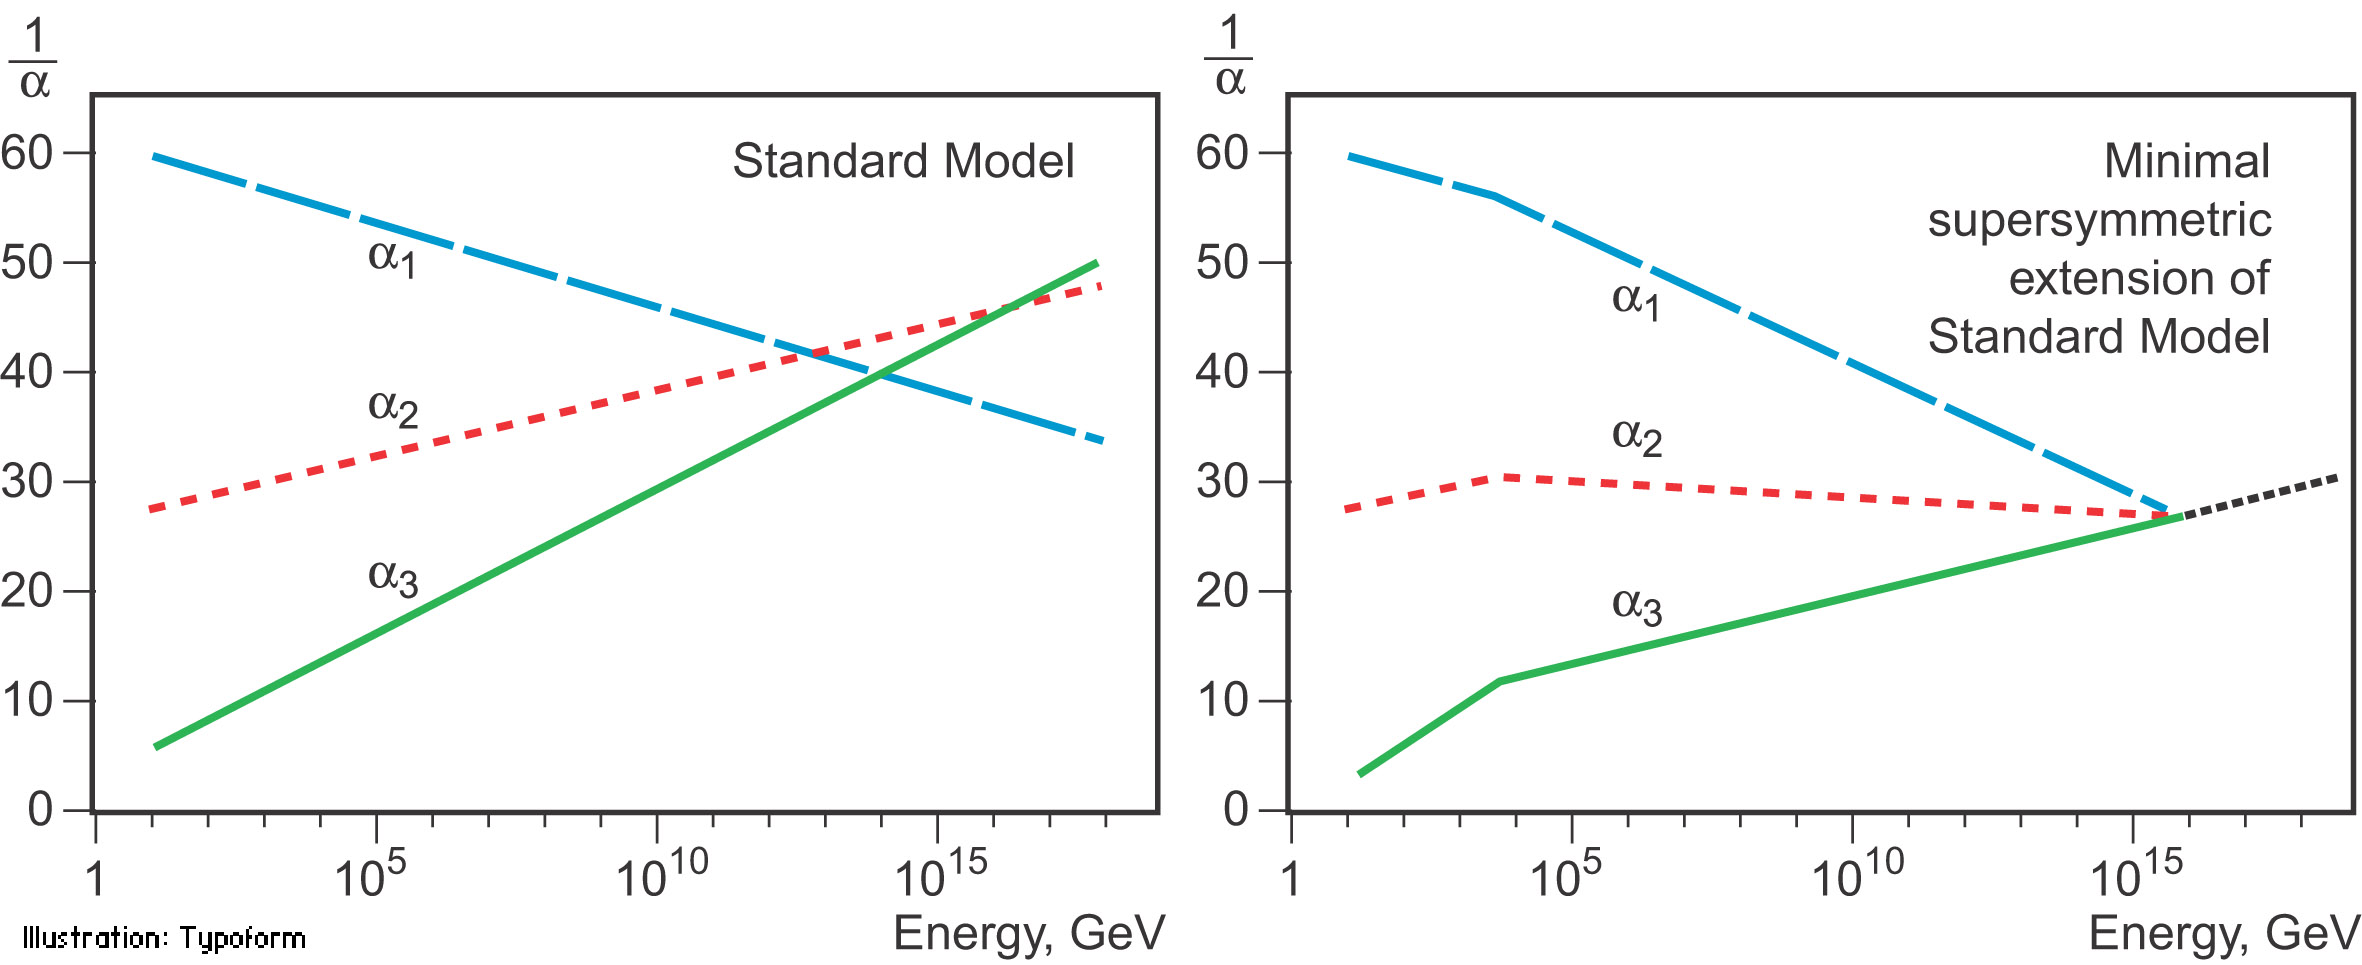
\includegraphics[width=1.0\linewidth]{figs/runningCouplingSusy}
  \caption[]%
  {Evolution of the inverse of the coupling constants of the
  electroweak $U(1)$, $\alpha_1$, electroweak $SU(2)$, $\alpha_2$, and
  strong force $SU(3)$, $\alpha_3$ for the \SM and \MSSM \cite{runningCoupling}}%
  \label{fig:runningCoupling}
\end{figure}

\subsection{The Minimal Supersymmetric Standard Model}
\label{sec:MSSM}

The \acf{MSSM} is a model that incorporates \SUSY with the \SM in a
way that adds the minimum number of new particles and interactions
\cite{Csaki:1996ks}. The \MSSM has 105 free parameters in total, a
significant increase from the 19 in the \SM. A summary of the extra
particles, \emph{sparticles}, introduced by the \MSSM is available in Tab.~\ref{tab:susy}.
The superpartners to the fermions are denoted with the same symbol as
their associated fermion with a tilde above. The weak sector is
extended within the \MSSM and the mixing of the new \SUSY fields
associated to the electroweak and Higgs bosons leads to
the existence of neutralinos, charginos and a total of five Higgs
bosons, including two that carry an electromagnetic charge. 
%Could add in more detail of the fields and things here but it's
%probably not relevant...

\begin{table}
\begin{tabular}{|l|c|c|c|}
%\hline 
Name & Sparticle & Spin & Charge, $q$ \\
\hline
Up-type squarks & $\tilde{u},\tilde{c},\tilde{t}$ & 0 & $+\frac{2}{3}$ \\
Down-type squarks & $\tilde{d},\tilde{s},\tilde{b}$ & 0 & $-\frac{1}{3}$ \\
Charged sleptons & $\tilde{e},\tilde{\mu},\tilde{\tau}$ & 0 & $\pm1$ \\
Sneutrinos & $\tilde{\nu_{e}},\tilde{\nu_{\mu}},\tilde{\nu_{\tau}}$ & 0 & 0 \\
\hline
%\hline
Gluino & $\tilde{g}$ & $\frac{1}{2}$ & 0 \\
Neutralinos &
$\tilde{\chi_{1}}^0,\tilde{\chi_{2}}^0,\tilde{\chi_{3}}^0,\tilde{\chi_{4}}^0$
& $\frac{1}{2}$ & 0  \\
Charginos & $\tilde{\chi_{1}}^{\pm},\tilde{\chi_{2}}^{\pm}$ &
$\frac{1}{2}$ & $\pm1$ \\
\hline
Neutral Higgs bosons & $h^0,H^0,A^0$ & 0 & 0 \\
Charged higgs bosons & $H^{\pm}$ & 0 & $\pm1$ \\
\end{tabular}
\caption{The extra particles introduced by the \MSSM. The symbol $h^0$
is typically used to denote the \SM Higgs boson.
% A subscript of
% $L$ or $R$ denotes the left or right-handed states respectively
\cite{Martin:1997ns}}
\label{tab:susy}
\end{table}
% table from mark

Unlike the \SM, the \MSSM permits lepton and baryon number violation,
the total numbers of leptons and baryons do not need to be conserved.
This could lead to interactions in which quarks can produce leptons,
such of interactions would allow protons to spontaneously decay.
However, stringent limits have been set on the lifetime of a proton,
$\tau>10^{33}$~years, that should exclude or heavily suppress this
kind of behaviour. This is dealt with in the \MSSM by introducing a
new conserved quantity known as \emph{R-parity}, $R$:
\begin{equation}
R\equiv (-1)^{3(B-L)+2s}
\end{equation}
where $B$ is the baryon number, $L$ the lepton number and $s$ the spin
of the particle. This leads to \SUSY particles having $R=-1$ and \SM
particles have $R=+1$. The consequence of this is that \SUSY particles
always decay to at least one other \SUSY particle. Additionally, any
\SUSY particles produced by \SM interactions must be produced in
pairs and vice versa. With R-parity conservation the \acf{LSP} is
stable. This fact allows it to fulfil the role of \DM in the case that
the \LSP is neutral. In most favoured \SUSY models the \LSP is
therefore typically taken to be a neutralino \cite{Farrar:1978xj}.
% R-parity - put a note on DM
% define lsp - neutralino in the case of DM

For the \MSSM to successfully solve the hierarchy problem an
additional constraint is applied to the \SUSY particles. As there is
no explicit mass hierarchy in the squark generations predicted in
\SUSY, the sparticles of the top-quark, the \emph{stop}, is typically
required to be the lightest of the squarks. This ensures maximal
cancellation of the contributions to the Higgs mass from the
top-quark, which couples most strongly to the Higgs in the \SM.
% light stops - to solve hierarchy problem

\subsection{Signatures of supersymmetry at the \LHC}

Despite the fact that \SUSY presents a promising extension to the \SM
there have been no significant experimental hints of its existence.
Searches for the evidence of \SUSY production have been performed in a
series of particle collider experiments, but have only resulted in
excluding possible regions of \SUSY parameter space. However, for
\SUSY to convincingly solve the hierarchy problem, it is expected to
present itself at the $O(1)$~TeV energy scale. This scale is just
starting to be explored by the \LHC. If \SUSY is to exist in the form
that is typically conceived it should therefore be evident in the
proton collisions produced by the collider.

The fact that there are a lot of different free parameters in the
\MSSM leads to a wide range of possible \SUSY phenomenologies.
However, constraints made by R-parity and naturalness
considerations help to limit the possible signatures. These
constraints typically lead to the pair production of \SUSY particles
that rapidly decay via \SM particles to a weakly interacting neutral \LSP. 
As the produced \SUSY particles have a reasonably high mass, this
leaves a significant missing momentum signature in any detector that
is looking for \SUSY signatures.
% R-parity, naturalness, neutralino lsp make it good for searching

As the \LHC is a hadron collider, the highest cross section \SUSY
production processes occur via the strong force \cite{Martin:1997ns}
\cite{SUSYxsections_NewAspectsof_pp_collisions}. These processes
result in the production of pairs of squarks or gluinos, the \SUSY
particles with colour charge, that predominantly decay via an even
number of \SM quarks to an \LSP. A Feynman diagram of typical squark
and gluino production and decay is shown in Fig.~\ref{fig:susyDecay}.
The resulting signature will usually be characterised by high energy
hadronic jets of \SM particles recoiling from invisible particles.

\begin{figure}
  \centering
  \subfloat[]{
    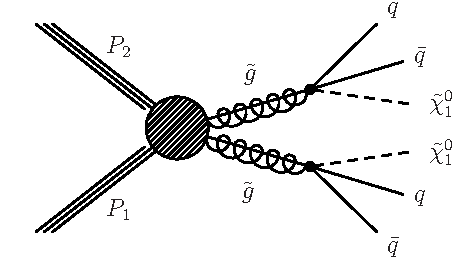
\includegraphics[width=0.4\textwidth]{figs/T1qqqq}
    \label{fig:susyDecayGluino}
  }~~~ 
  \subfloat[]{
    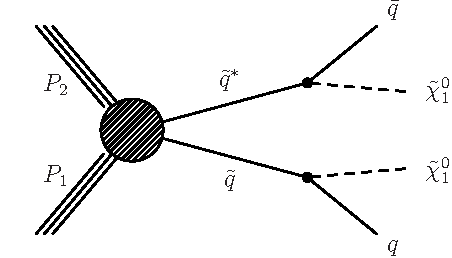
\includegraphics[width=0.4\textwidth]{figs/T2qq}
  }
  \caption{Representative \SUSY production and decay of gluinos, (a), or
  squarks, (b), in proton-proton collisions. The \SUSY particles decay
  to a weakly interacting neutralino, $\tilde{\chi_1}^0$, via \SM
  quarks \cite{smsTwiki}.}
  \label{fig:susyDecay}
\end{figure}

\subsection{Simplified models}

As there are a large number of parameters in the \MSSM there are many
different versions of the theory that can all result in different
\SUSY phenomenology. One of the things that has the biggest effect
when carrying out searches for \SUSY production is the mass hierarchy
of the particular model. To help to rationalise this the results of
\SUSY searches are typically interpreted within the context of
\emph{simplified models} \cite{Alwall:2008ag,Alves:2011wf}. These
models utilise a \SMS framework that typically consider only one
possible \SUSY decay per model. The simulated \emph{parent} \SUSY
particles and the \emph{daughters} that they decay to are kept at a
reasonable mass scale that is reachable by the search. All other \SUSY
particles are assumed to be at a much higher mass scale such that they
have no effect on the decay in question. An example of a decay
targeted by a simplified model with gluino parents and neutralino
daughters is in Fig.~\ref{fig:susyDecayGluino}. 

Searches for \SUSY are typically interpreted in different simplified
models with a wide range of parent and daughter masses. In the case
that no \SUSY signature is observed, the simplified models that are
excluded and those that are not allow limits to be set on the minimal
mass of different \SUSY particles within the context of the particular
simplified model. As the models separate out different possible \SUSY
production and decay mechanisms searches will typically interpret
their results in different models. Searches that look in a purely
hadronic final state, for example, will consider simplified models
that do not have leptons in the final state. Also, the type of search
that is successful at excluding some types of mass spectra is not as
successful at others. When the parent and daughter particles are very
close in mass, known as having a \emph{compressed spectrum}, the \SM
decay products carry very little energy. Searches for these types of
models therefore rely on \acf{ISR} or \acf{FSR} recoiling from the
invisible \SUSY system.

% With the standardised \SMS framework the interpretation of the results
% of \SUSY searches across the whole field is made simpl
%easy for outside interpretation

\subsection{Status of experimental searches for supersymmetry}

Signatures of \SUSY have been extensively searched for at previous
particle collider experiments including HERA ($ep$)
\cite{Aid:1996es,Butterworth:1992tc}, LEP ($e\bar{e}$)
\cite{Braibant:2003px} and the Tevatron ($p\bar{p}$)
\cite{Jaffre:2012gx}. These were then surpassed in most regions of
phase space by searches with the \CMS and ATLAS experiments with the
\LHC during Run~1. The \LHC is the first experiment to prove the
multi-TeV scale, where natural \SUSY is expected to lie. No hints of
\SUSY have yet been seen. The degree to which the $8~\tev$ Run~1
results have excluded the mass scales of different \SUSY particles
within a simplified model context can be seen in
Fig.~\ref{fig:run1Exclusion}.
%show lhc1 thing

\begin{figure}
  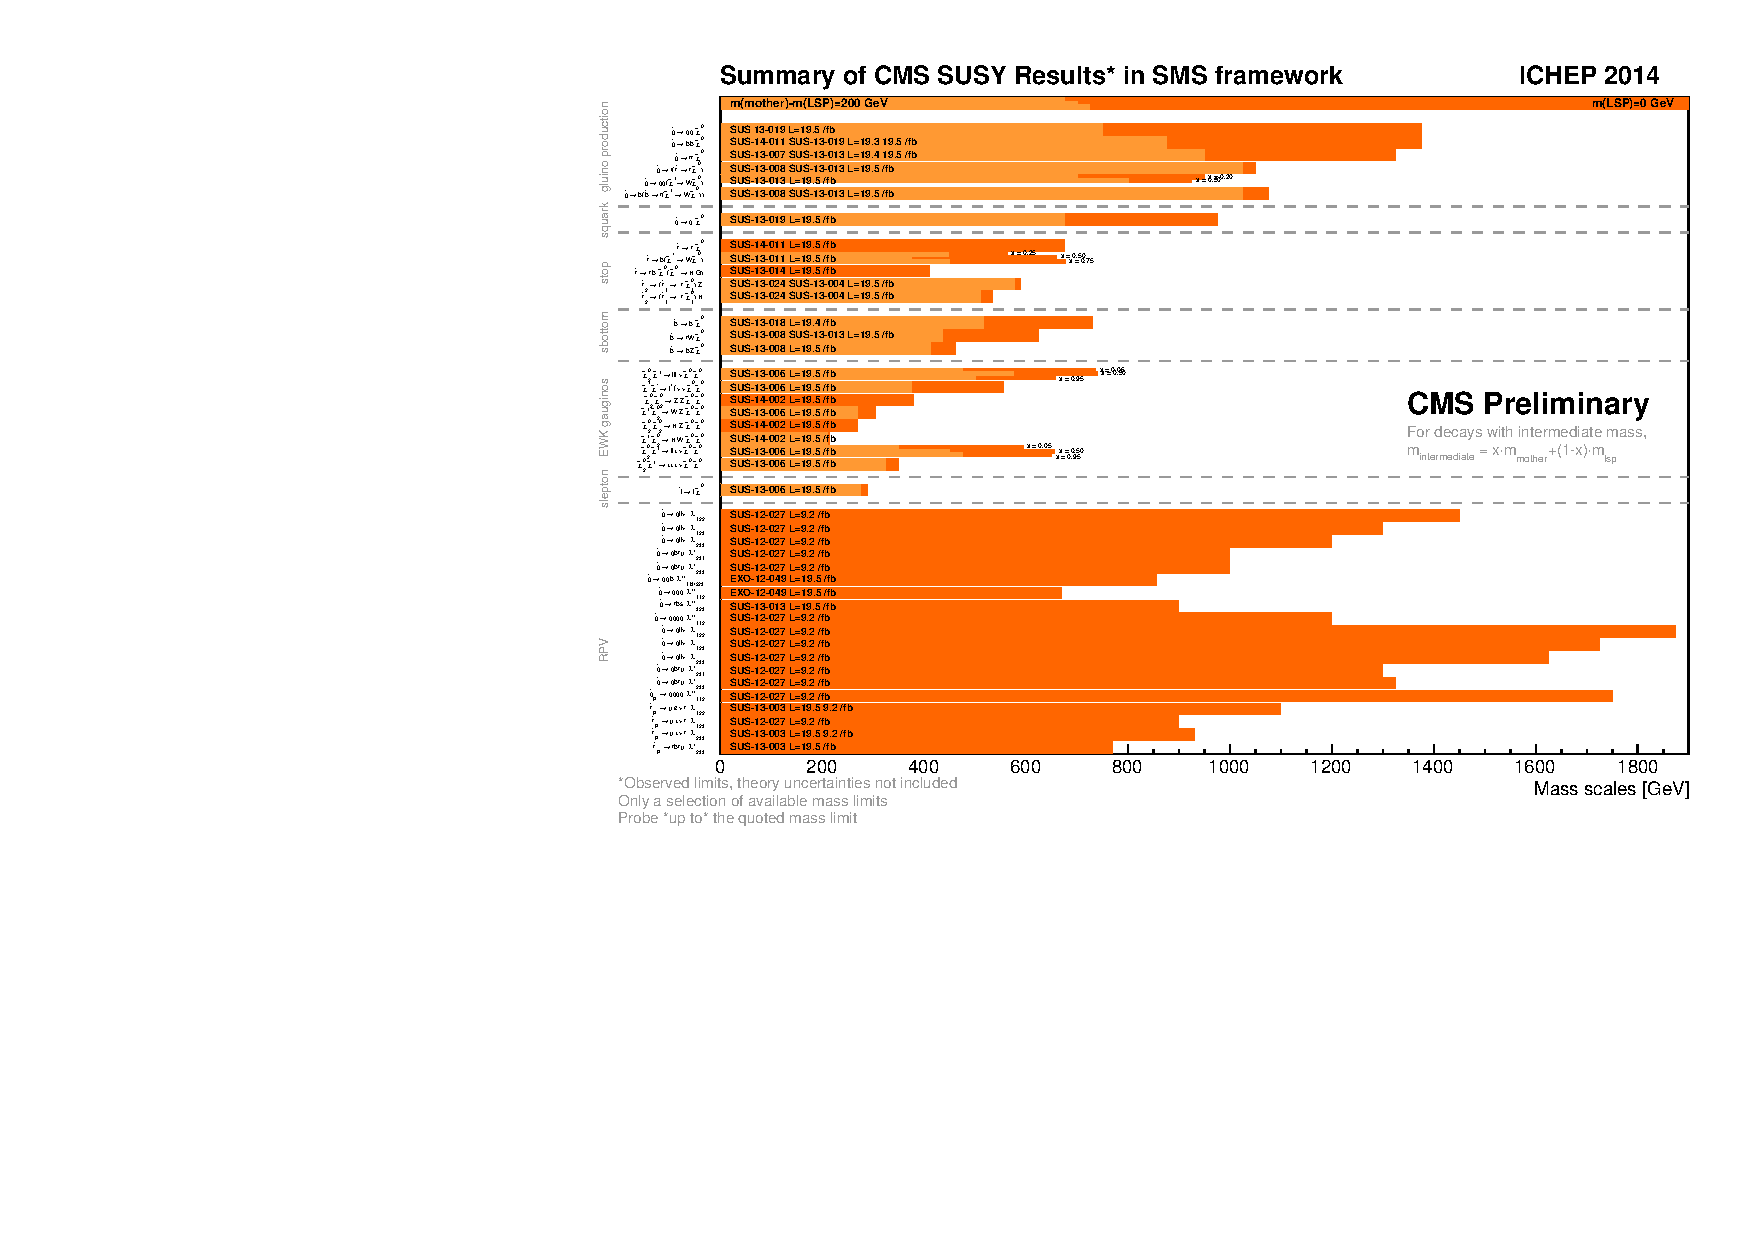
\includegraphics[width=1.0\linewidth]{figs/run1SusyExclusion}
  \caption[]%
  {Maximum exclusion limits for the mass of \SUSY parent particles for
  simplified models with an \LSP with 0~GeV mass (dark shades) or
  parent mass minus \LSP mass of 200~GeV (light shades) for a
  representative selection of simplified model topologies. The results
  were made with data collected by \CMS with $8~\tev$ centre of mass
  proton-proton collisions \cite{smsTwiki}.}%
  \label{fig:run1Exclusion}
\end{figure}

% Best exclusion limits for the masses of the mother particles for
% m(LSP) = 0 GeV (dark shades) and m(mother) - m(LSP) = 200 GeV (light
% shades); for each topology, for all results. In this plot, the lowest
% mass range is m(mother)=0, but results are available starting from a
% certain mass depending on the analyses and topologies. Branching
% ratios of one are assumed, values shown in plot are to be interpreted
% as upper bounds on the mass limits, see the analyses documentations
% for details. (Note: theory uncertainties not included.)

For \SUSY at the electroweak scale to exist in a sensible form that
convincingly solves the problems described in Sec.~\ref{sec:bsm} it
should be observable during Run~2 of the \LHC that probes even higher
energies with $13~\tev$ proton collisions. If no evidence presents
itself, the typical assumptions made when building \SUSY models will
have to be reassessed.


  \chapter{The CMS experiment at the LHC}
\label{chap:detector}

\chapterquote{Traditional scientific method has always been, at the
very best, 20-20 hindsight. It's good for seeing where you've been.
It's good for testing the truth of what you think you know, but it
can't tell you where you ought to go.}%
{Robert M. Pirsig, Zen and the art of motorcycle maintenance}

The \LHC is one of the largest machines ever built. It exists within a
27~km tunnel $\sim 100$~m$)$ underground on the border of France and
Switzerland. Around the ring of the \LHC are built a series of
detectors that can record in a high level of detail the result of high
energy particle collisions produced by the collider. This chapter
will focus on the details and performance of \CMS, a multi-purpose
detector optimised to search for new, as yet undiscovered, particles.

\section{The LHC}
\label{sec:lhc}

The \LHC is a hadron collider designed to collide protons and lead
ions at centre of mass energies up to 14\tev, the highest ever achieved by such a
machine
\cite{Evans:2008zzb,CERN-2004-003-V-1,CERN-2004-003-V-2,CERN-2004-003-V-3}.
The proton-proton collisions are most utilised for direct searches for
new physics and therefore take up the vast majority of the \LHC's
running time. 

To bring protons up to the $6.5~\tev$ required in Run~2 of the \LHC
they are accelerated through a series of stages. Hydrogen atoms are
initially stripped of their electrons and accelerated to 50\mev by
\ac{LINAC2}. The energy is then increased to 1.4\gev by the \ac{PSB}
before being injected into the \ac{PS} which boosts the energy up to
26\gev. A final kick up to 450\gev is provided by the \ac{SPS}. This
chain of accelerators also collect the protons into bunches that are
either 25~ns (from Run~2 onwards) or 50~ns apart (during Run~1 and
early stages of Run~2). These bunches are then injected into the \LHC,
in which they are steered by around 1200 superconducting dipole
magnets while being accelerated up to $6.5\tev$ with \ac{RF} cavities.
Once the beam has reached the intended energy and is stable, protons
are collided at four different points on the ring, around which are
built the four major \LHC detectors, ALICE \cite{Aamodt:2008zz}, ATLAS
\cite{Aad:2008zzm}, LHCb \cite{Alves:2008zz} and \CMS
\cite{Chatrchyan:2008aa}.  A representation of this accelerator
complex and the location of the detectors can be seen in
Fig.~\ref{fig:lhc}.

\begin{figure}
  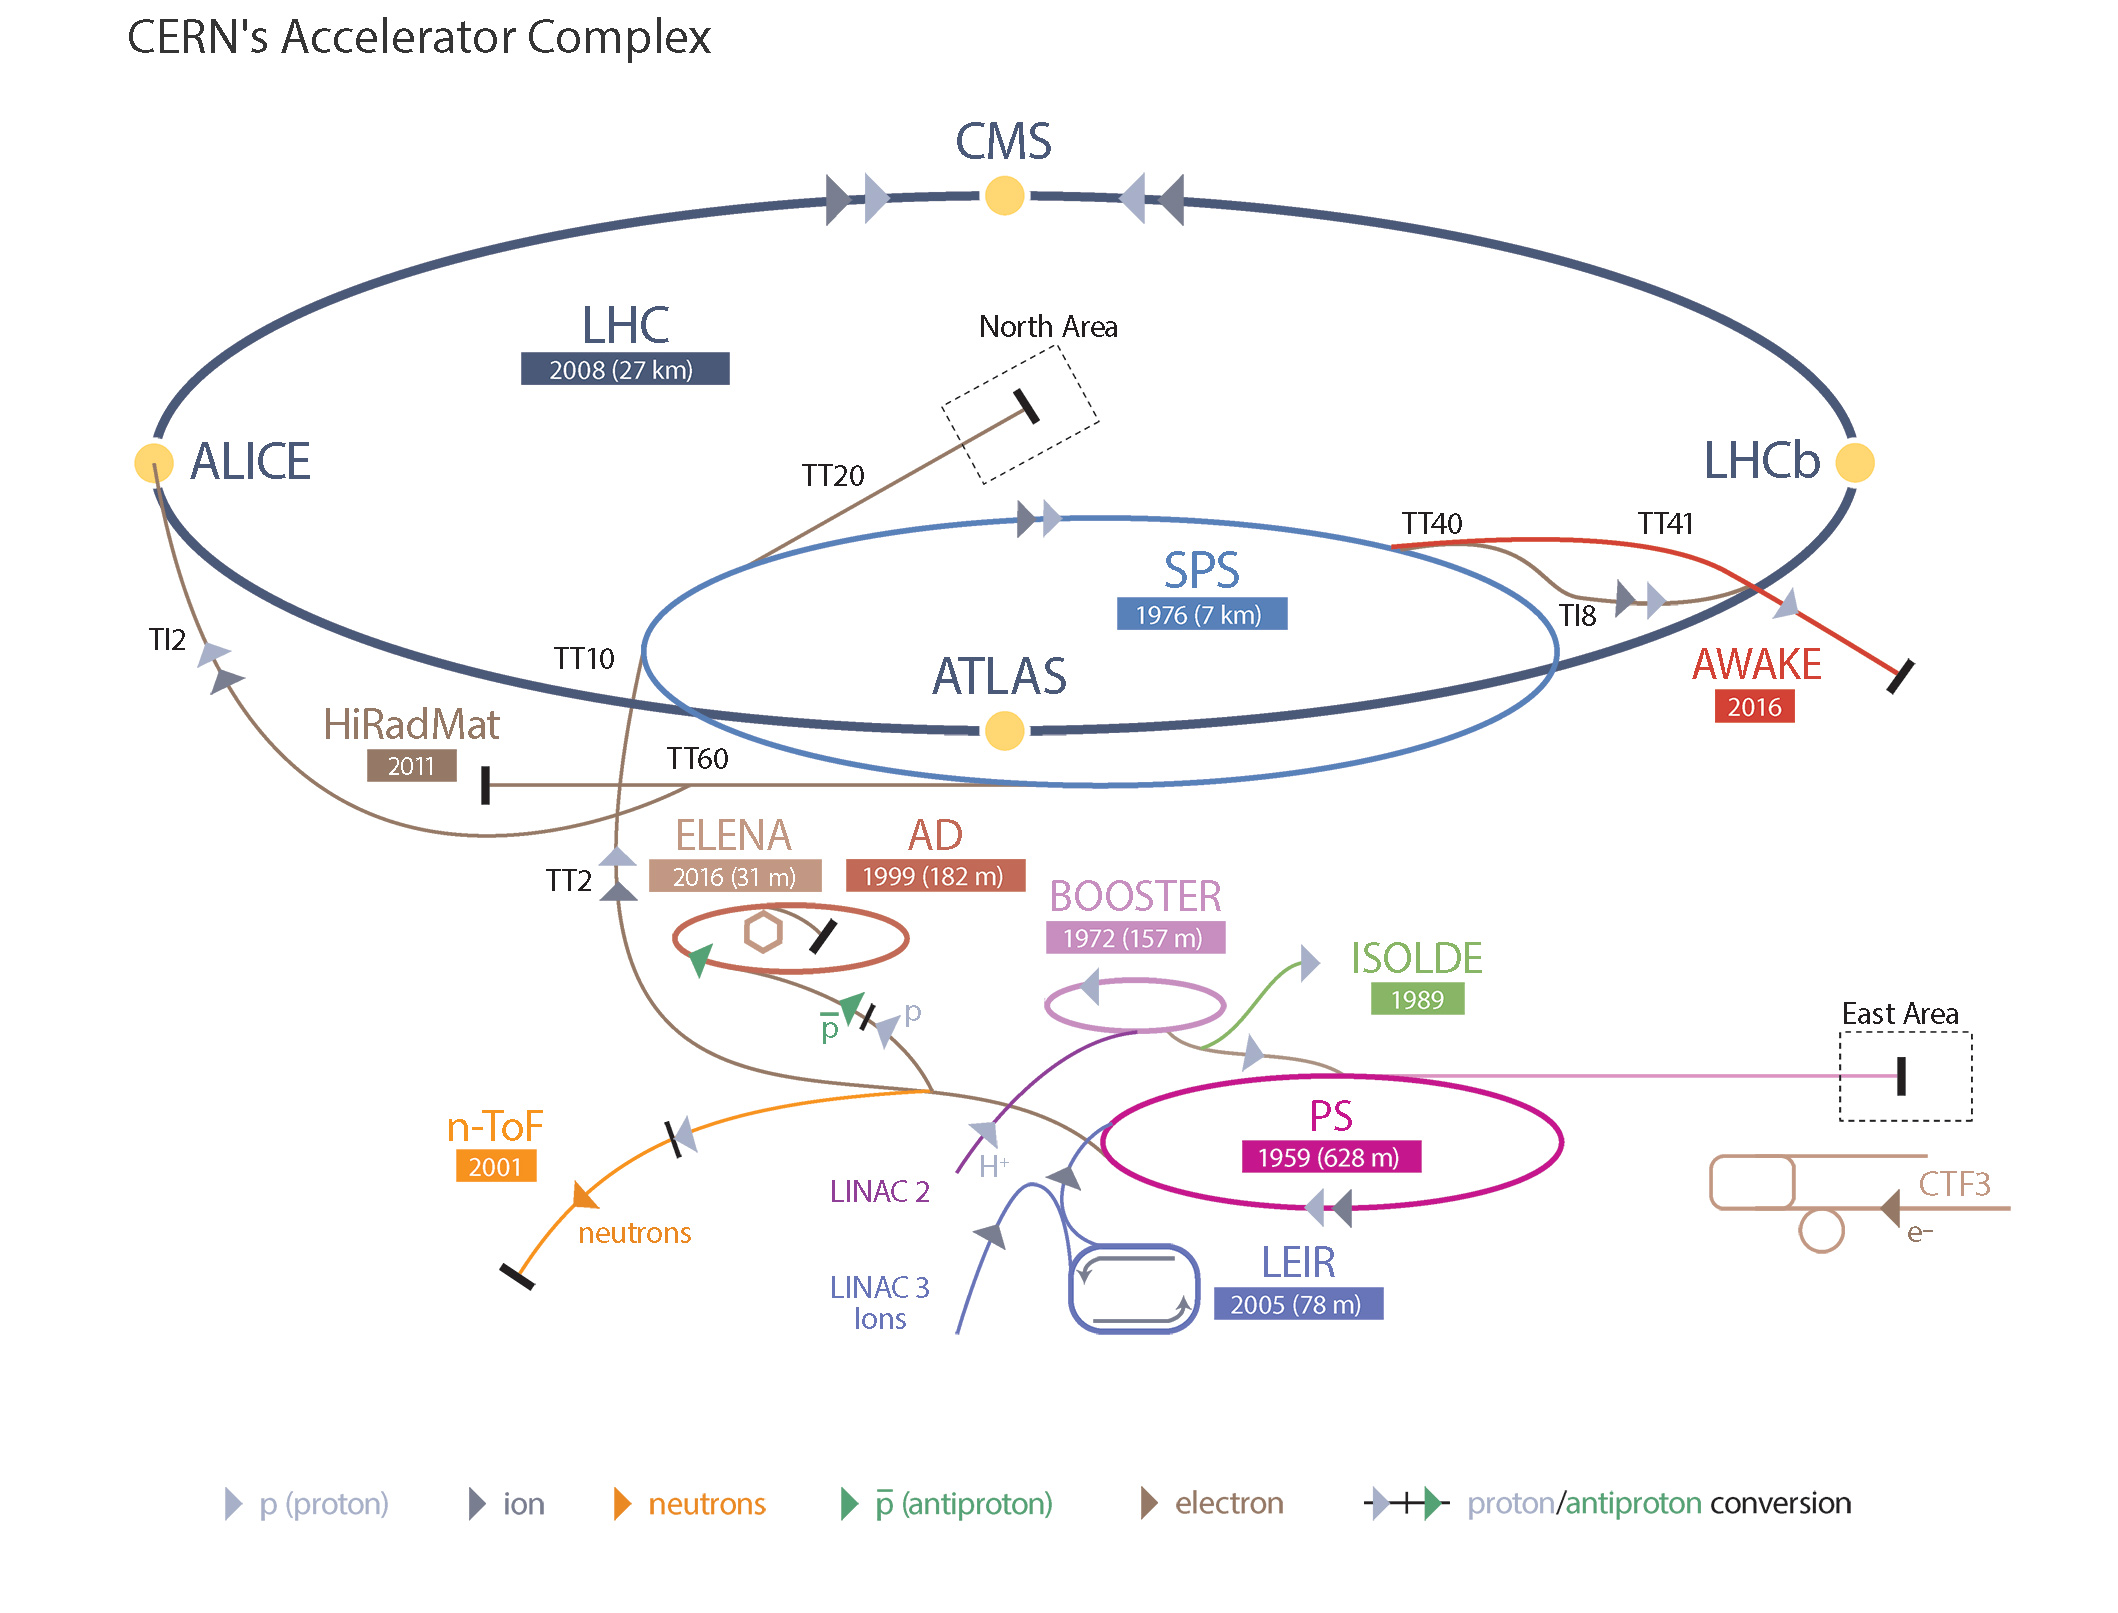
\includegraphics[width=\largefigwidth]{figs/LHC_default}
  \caption[]%
  {A representation of the CERN accelerator complex that help
  accelerate protons to record energies within the \LHC
  \cite{stfc:lhc}}%
  \label{fig:lhc}
\end{figure}

As well as attaining record breaking energies, the \LHC is designed to
collide hadrons at a very high luminosity, with a bunch collision rate
of up to $40~\mhz$ \cite{Evans:2008zzb}. This is necessitated by the
fact that the rate at which electroweak scale processes
occur in proton collisions is significantly lower than their
associated backgrounds, demonstrated in Fig.~\ref{fig:xsecs}.
The \LHC is therefore designed to run at an instantaneous
luminosity approaching $10^{34}$cm$^{-2}$s$^{-1}$ to maximise the occurence of
these rare processes. Along with the high collision rate, this
luminosity is achieved by squeezing the proton bunches to increase the
number of simultaneous collisions per bunch crossing, the extra
simultaneous collisions are known as \PU.  The \LHC has typically
operated with a \PU of $\sim10\mbox{-}20$, however to increase the
luminosity in the future this value will be increased up to a \PU of
O(100).
% , presenting a significant challenge for current and future 
% physics analyses at the \LHC.

\begin{figure}
  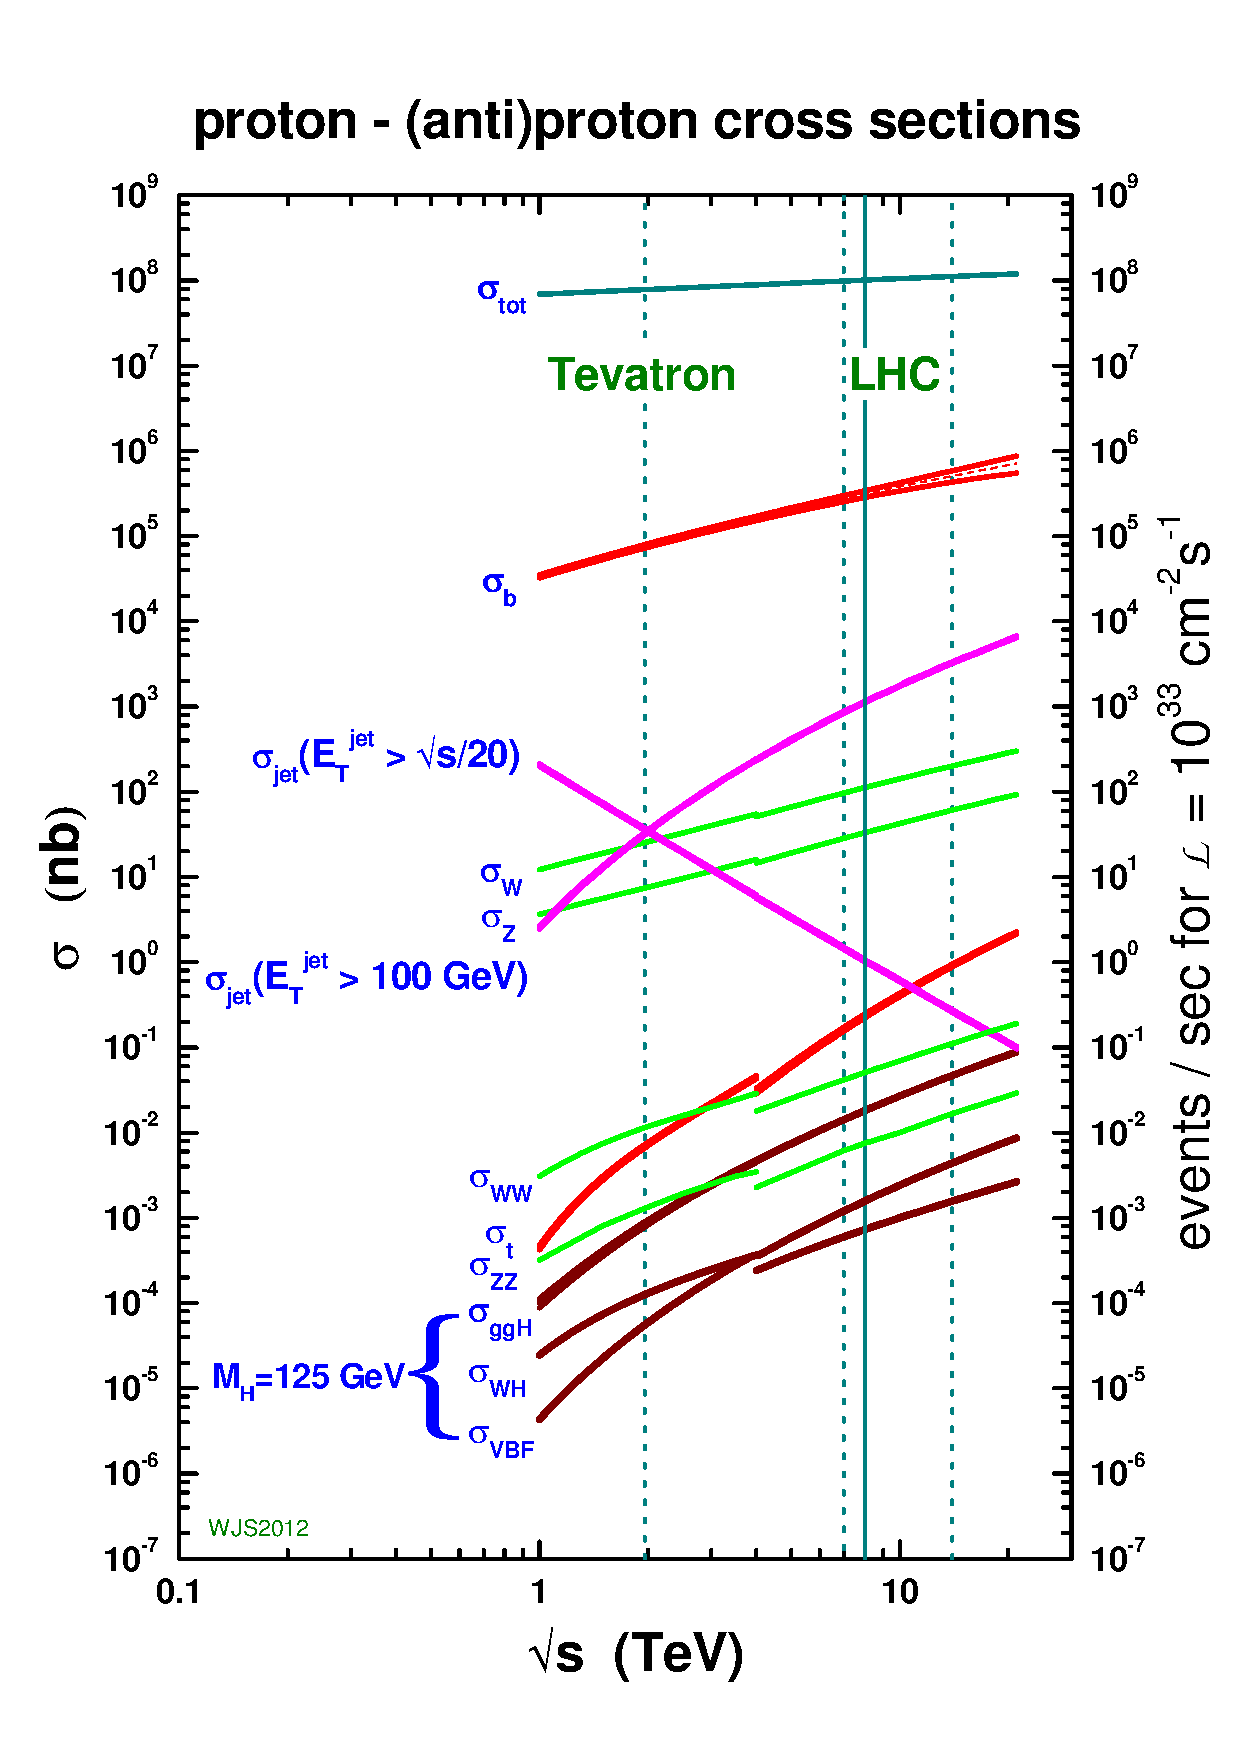
\includegraphics[width=\mediumfigwidth]{figs/crosssections2012_v5}
  \caption[]%
  { The cross sections for various standard model processes as a
  function of proton collider energy, demonstrating the importance of
  high luminosities when observing electroweak scale processes
  \cite{stirlingCrossSec1}.}%
  \label{fig:xsecs}
\end{figure}

During Run~1 of the \LHC, from 2010-2013, a total of $23.3~\ifb$ of
data were collected at centre of mass energies of $\sqrt{s}=7~\tev$ and
$8~\tev$. After this there was a period of shutdown in which the \LHC
and the detectors underwent a series of upgrades. Run~2 then began in
2015 with the collision of protons at $\sqrt{s}=13~\tev$. During 2015 a
total of $4.3~\ifb$ were collected at this energy. So far in 2016 the
\LHC has delivered $34.6~\ifb$, a record breaking number of collisions
at the highest ever recorded energies. 

\section{The CMS detector} \label{sec:cms}

The \CMS detector is one of two multipurpose detectors built around
proton beam collision points, the other being ATLAS. It is situated at
Point 5 on the \LHC, as visibile in Fig.~\ref{fig:lhc}. The key goals
of the \CMS detector at its conception were the discovery of the \SM
Higgs boson and searches for generic signatures of \BSM physics. In \CMS the
results of collisions are measured with a series of subdetectors,
built within and around a $3.8~$T superconducting solenoid. They are designed to
track, identify and record the energy of all non-neutrino \SM particles
\cite{Bayatian:2006zz}. With its comprehensive solid
angle coverage, \CMS is well suited to inferring the existence of
weakly interacting particles through the momentum imbalance of visible
particles. This is particularly relevant when searching for \BSM
physics.

\begin{figure}
\begin{center}
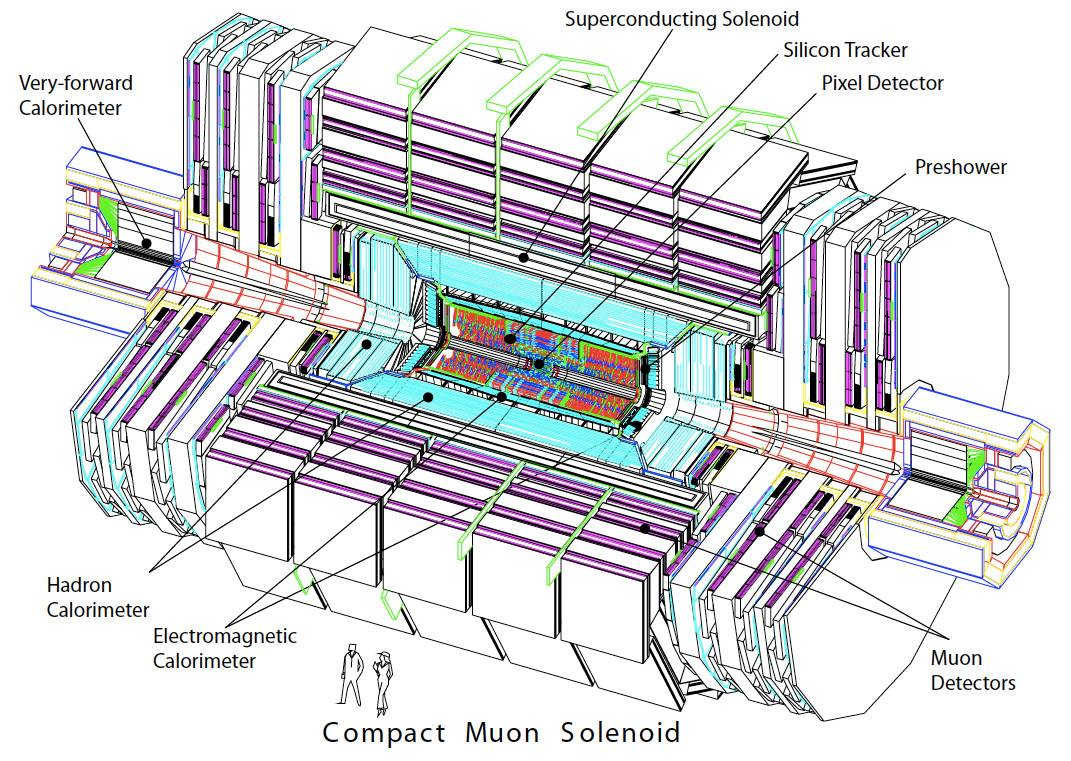
\includegraphics[width=0.8\linewidth]{figs/cms_detector} \end{center}
\caption{An internal view of the \CMS detector
highlighting the key detecting components \cite{Bayatian:2006zz}}
\label{fig:CMS} \end{figure}

A representative view of \CMS and its components can be seen in
Fig.~\ref{fig:CMS}. The detector is designed in a series of
cylindrical layers of subdetectors working out from the central point,
where the proton collisions occur. The first layer consists of the
silicon tracking system. This tracker is designed to allow the
reconstruction of the trajectory of charged particles produced in the
collision point as they move through the magnetic field. The degree to
which the path of these particles is bent allows for an accurate
determination of their momenta. The next layer beyond the silicon
tracker is the \ECAL, which is designed to absorb and measure the
energy of electrons and photons. Surrounding this is the \HCAL that
absorbs the remaining hadronic particles that have punched through the
\ECAL. Built around the tracker and calorimeters is the superconducting
solenoid. In the final layer are the muon chambers and iron return
yoke. The chambers are designed to detect the presence of muons that
will not be absorbed by the central components of the detector. The
data from all these subdetectors are read out by dedicated front end
electronic. They are then passed through the \CMS trigger system which
selects the most promising data to be kept and stored for ``offline''
processing. 

Measurements of physical quantities made by \CMS are typically
interpreted in a three dimensional coordinate system that originates
from the centre of the detector. The $x$-axis points south, to the
centre of the \LHC ring, the $y$-axis points vertically upwards and
the $z$-axis points along the direction of the \LHC beam pipe. It is
then helpful to define the azimuthal angle $\phi$ which is in the
$x$-$y$ plane and measured relative to the $x$-axis. Measurements of
momentum and energy in this plane are described as transverse and
known as \pt and \Et respectively. The polar angle $\theta$ is then
defined as relative to the $z$-axis. This angle is used to construct
the pseudorapidity, defined as $\eta=-ln(tan(\theta/2))$. Distances in
the $\eta$-$\phi$ plane is then given as $\Delta R =
\sqrt{\Delta\phi^2+\Delta\eta^2}$.

\subsection{The tracker} 

The \CMS inner tracking system is designed to accurately determine the
trajectories of charged particles produced in hadron collision events
\cite{Karimaki:368412}. In the presence of the strong magnetic field
provided by \CMS's solenoid, the curvature of these tracks can be used
to reconstruct momenta with a resolution between $1.5\%$ and $3\%$ for
$p_T\sim 100$~GeV charged particles. The tracker is also capable of
tracking \mbox{$p_T>1$~GeV} charged particles with an efficiency
greater than $99\%$ \cite{Bayatian:2006zz}. Along with this, the
spatial resolution of the tracker is such that the points of origin of
event decay products can be inferred within $10$~$\mu$m. Together,
this allows the performance of \CMS to extend up to very high levels
of \PU.% \cite{CMSTrackPerformance}.

The tracker is required to operate in a challenging, high radiation
environment. Additionally, in an ideal detector the particles produced
in collisions are solely absorbed by the calorimeters. The tracker
must therefore consist of as little material as possible. To achieve
the high level of precision and fast response time required given
these conditions, the tracker utilises silicon technology. As charged
particles pass through doped silicon an electron-hole pair is
produced. In the presence of an electric field this gives rise to a
pulse of electrical current in the previously resistive silicon. This
behaviour is utilised by the tracker in a series of silicon pixel and
strip detectors covering all angles in \phi and extending up to
$|\eta|<2.5$. The tracker's layout is visible in
Fig.~\ref{fig:tracker}. 

\begin{figure}
\begin{center}
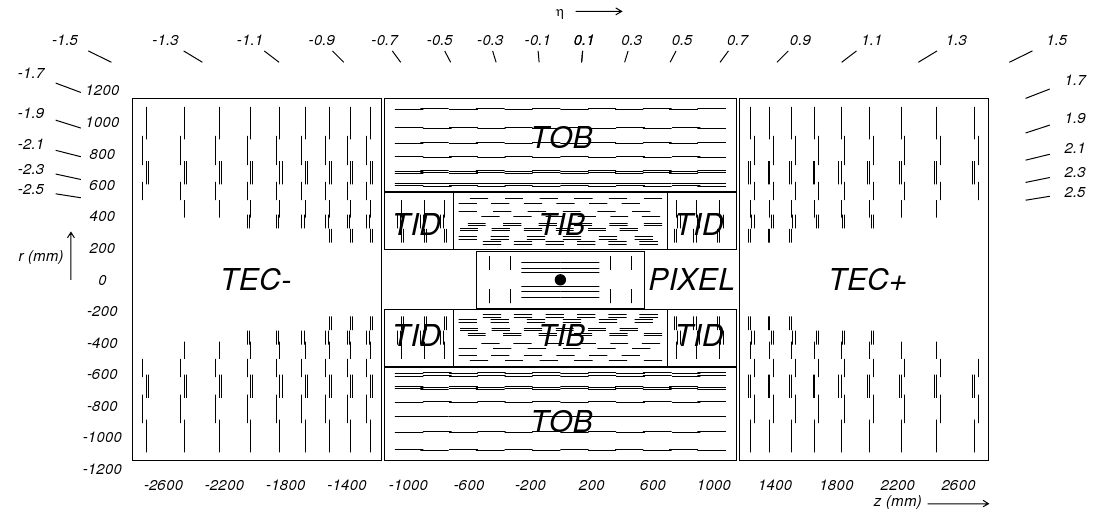
\includegraphics[width=0.8\linewidth]{figs/cmstracker} \end{center}
\caption{ A schematic of a cross section through the \CMS tracker.
Detector modules are represented by different lines \cite{Chatrchyan:2008aa}}
\label{fig:tracker} \end{figure}

The pixel detector is the high granularity component of the tracking
system that sits closest to the interaction point, covering the
pseudorapidity region $|\eta|<2.5$. It consists of three cylindrical
layers of hybrid pixel detector modules that are complemented by two
disks of pixel modules on each side. The pixel detector makes use of
66 million pixels covering an area of $\sim 1$~m$^2$ to give the
tracker its excellent spatial resolution of $15$-$20$~$\mu$m in both
the $r$-$\phi$ and $z$ direction. This resolution is essential for a
precise determination of the position of collision event vertices and
for the observation of vertices displaced from this origin that can be
used to identify particles such as hadrons containing $b$-quarks.

Surrounding the pixel detector is the silicon strip tracker that
covers the region up to $|\eta|<2.4$. It consists of three different
subsystems built from 9.6 million silicon strips that cover an area of
198~m$^2$. Each of these strips are 10-20~cm long and 80-180~$\mu$m
wide. Working out from the centre the subsystems are the
Tracker Inner Barrel and Disks (TIB/TID), the Tracker Outer Barrel
(TOB) and the Tracker End Caps (TEC). They are arranged in a geometry
that maintains a good degree of coverage across all angles and can be
seen in detail in Fig.~\ref{fig:tracker}. Along with the spatial
resolution provided by the pixel detector the silicon strip tracker
adds enough modules to reconstruct the trajectory of particles to the
required high level of precision.

\subsection{The electromagnetic calorimeter} 

The \ECAL is constructed from $\sim 75~848$ lead tungstate (PbWO$_4$)
scintillating crystals covering the region $|\eta|<3$ \cite{CMS:1997ema}. It is
designed to absorb electrons and photons and emit light proportional to the
energy deposited. This light is detected by custom photodiodes that
perform well in high magnetic fields. This is achieved in a way which
is fast, radiation resistant and with a high granularity. 

The \ECAL is divided into the \ac{EB} which covers the region
$|\eta|<1.479$ and the \ac{EE} which covers the region
$1.479<|\eta|<3.0$. Additionally, built just before the \ac{EE} in the
region $1.653<|\eta|<2.6$ is the Preshower. Unlike the other
components, which are predominantly PbWO$_4$ crystals, the Preshower is
a lead and silicon sampling calorimeter. Its main aim is to improve
the position resolution of particles in the forward direction and help
to distinguish collinear $\pi^0$ decays from high energy photons
\cite{Chatrchyan:2008aa}. This layout of the \ECAL can be seen in
Fig.~\ref{fig:ecal}.

\begin{figure}
\begin{center}
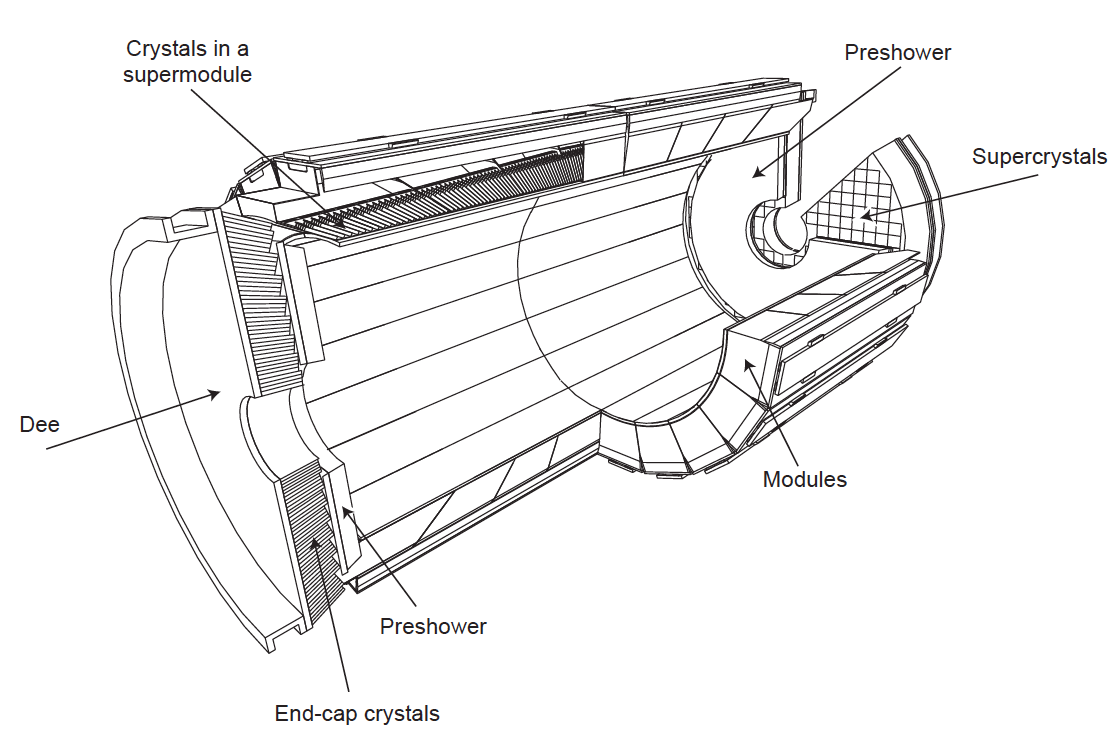
\includegraphics[width=0.8\linewidth]{figs/ecal_colorless} \end{center}
\caption{ A cutaway diagram of the \CMS \ECAL. All the key components,
including the barrel and endcap crystal layouts, are displayed
\cite{Chatrchyan:2008aa}}
\label{fig:ecal} \end{figure}

As high energy electrons or photons enter one of the \ECAL's crystals
they initiate an electromagnetic shower. This results in a cascade of
lower energy particles that undergo bremsstrahlung and pair
production.  These charged particles ionise atoms in the crystal which
then emit scintillation light as they de-excite. As the crystals are
transparent, this light can be measured by avalanche photodiodes and
vacuum phototriodes which convert it into an electronic current. The
magnitude of this current is then proportional to the energy deposited
in the crystal and can be used to accurately infer the total energy
deposited. Irradiation of the crystals decreases their transparency
over time. To counteract this a time dependent calibration is carried
out for each of the crystals with a laser of wavelength
$\lambda=440$~nm. 

Measurements in a test beam in the absence of a magnetic field have
measured the PbWO$_4$ crystals to have a resolution, $\sigma_E$, given
by the following formula \cite{1748-0221-2-04-P04004}:
\begin{equation} \label{eq:ecalres}
\left(\frac{\sigma_E}{E[\gev]}\right)^2=\left(\frac{2.8\%}
{\sqrt{E[\gev]}}\right)^2+\left(\frac{12\%}{E[\gev]}\right)^2+(0.30\%)^2.
\end{equation} 
In this equation $E$ denotes the energy of the incident
particle. The first term encapsulates uncertainties from fluctuations in the
scintillation light. The second term takes account of noise in the
electronics and digitisation. The final term then covers any
non-uniform longitudinal response or inter-calibration errors. 

\subsection{The hadronic calorimeter} 

The final layer of calorimetry in \CMS is the \HCAL \cite{CMS:HCAL}.
It is designed to absorb hadrons that have punched through the \ECAL.
It is a sampling calorimeter that is constructed from brass absorbers
interleaved with scintillating plastic tiles covering $|\eta|<3$. The
scintillations are read out with hybrid photodiodes via wavelength
shifting fibres.  Additionally, the hadronic calorimetry is extended
up to $|\eta|<5.2$ with the \ac{HF}, made from steel absorber with
quartz scintillating fibre. 

The brass absorbers are arranged in plates that are interspersed with
plastic tiles. Incident particles induce hadronic showers in the
brass layers that produce scintillating light in the plastic. This
light is collected by wavelength-shifting fibres which transfer the
signal to on-detector amplifiers for read-out. Brass has the advantage
of being non-magnetic and having the short nuclear interaction length
of 16.42~cm. In the \ac{HF} steel replaces the brass and quartz fibre
replaces the plastic due to the very high radiation environment
present in the forward region of the detector. The total time to
collect a \HCAL signal pulse is large with respect to the collision
rate of the \LHC. Only $68\%$ of the pulse is collected within 25~ns.
This leads to cases of \ac{OOTPU} where signal from a bunch
crossing can influence the read out of future bunch crossings.

The subdetectors that make up the \HCAL along with the \ac{HF} can be
seen in Fig.~\ref{fig:hcal}. Within \CMS's solenoid is the \ac{HB},
which extends up to $|\eta|<1.3$, and the \ac{HE}, covering
$1.3<|\eta|<3.0$. They are segmented in \eta-\phi towers with a size
of $0.087\times0.087$ in the \ac{HB} varying up to $0.17\times0.17$ in
some areas of the \ac{HE}. The \ac{HB} towers are lined up with
$5\times5$ arrays of \ECAL crystals and each read-out individually. On
its own the \ac{HB} provides between $5.8$ and $10.6$ interaction
lengths of absorber while the \ac{HE} provides $\sim10$ interaction
lengths. Beyond the magnetic coil is the \ac{HO} that increases to a
minimum of $11.8$ the interaction length in line with the \ac{HB}. The
magnetic coil acts as an absorber for the scintillators in the \ac{HO}
that absorbs any late-starting or highly-penetrating showers.

\begin{figure}
\begin{center}
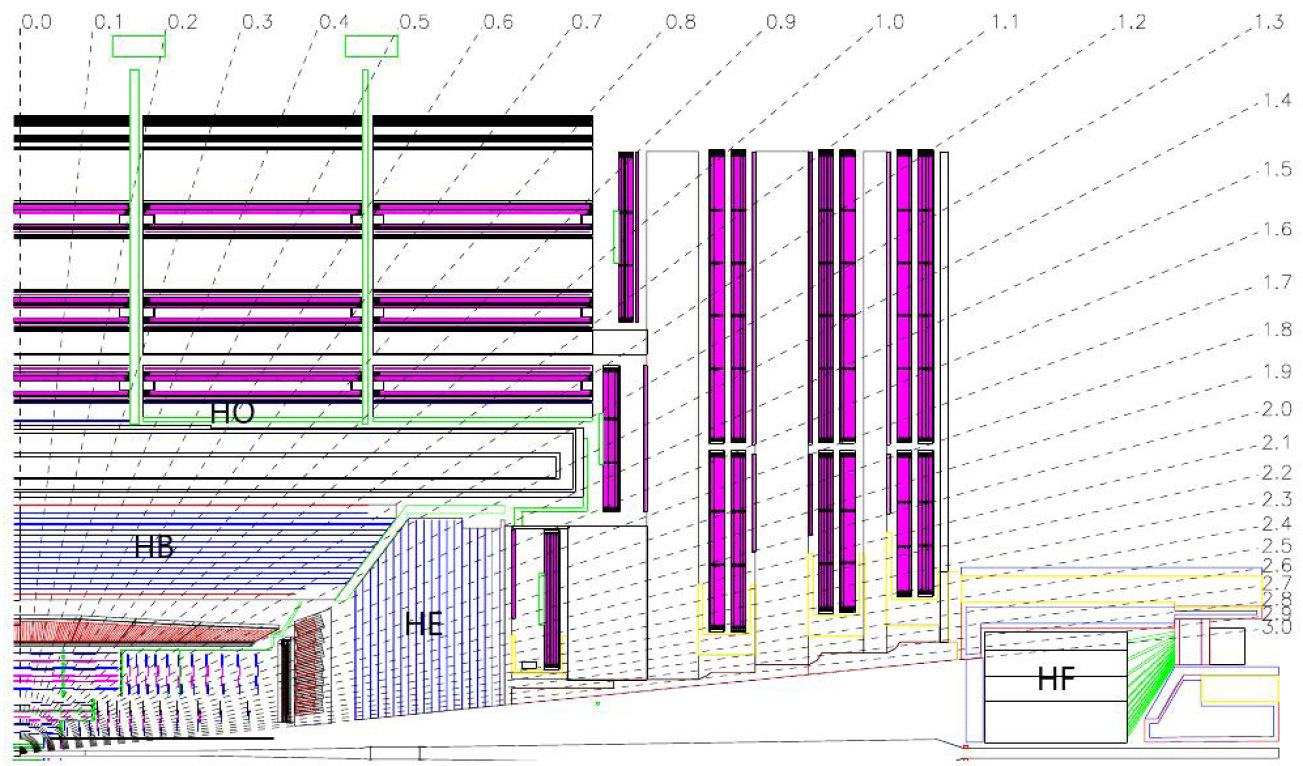
\includegraphics[width=0.8\linewidth]{figs/cms_HCAL} \end{center}
\caption{ A schematic of the \CMS \HCAL. The locations of the hadron
barrel (HB), endcap (HE), outer (HO) and forward (HF) calorimeters are
displayed \cite{Chatrchyan:2008aa}}
\label{fig:hcal} \end{figure}

The combined resolution, $\sigma_E$ of the \ECAL and \HCAL when
considered together have been measured in a test beam as
\cite{Abdullin:2008zzb}: 
\begin{equation} \label{eq:hcalres}
\left(\frac{\sigma_E}{E[\gev]}\right)^2=\left(\frac{84.7\pm1.6\%}
{\sqrt{E[\gev]}}\right)^2+(7.4\pm0.8\%)^2.  
\end{equation} 
In this equation $E$ is the energy of the incident particle. An
in-situ calibration is also performed with a UV laser and
$^{137}$Cs$/^{60}$Co sources that can be inserted into the scintillation
tiles in the \ac{HB} and \ac{HE}.

\subsection{The Muon System} As muons are unlikely to be absorbed in
the \ECAL and \HCAL, a muon system is built into the iron return yoke
that surrounds the solenoid.  This consists of wire chambers
containing ionising gas that allows the measurement of muon momenta
with a greater than $1\%$ precision
\cite{CMS_Overview_Chatrchyan:2008aa}.

\subsection{The Trigger and Data Acquisition System}
\label{sec:triggers} The rate of collisions at the LHC is so high that
it would be impossible to reconstruct and store the results of all
collision events. As the majority of the collisions are soft QCD
processes, they are not useful in the search for new physics at the
electroweak energy scale. This necessitates a multi-level trigger
system that is designed to pick out and store only high centre-of-mass
physics processes. The Level 1 Trigger (L1T) is the first component of
the trigger system and is made from custom FPGA computational boards
situated close to the detector. This uses coarse information from the
calorimeters and muon system to reduce the event rate from $20$MHz
(during Run 1) to $\sim100$kHz. The data from the subdetectors are
then passed to the High Level Trigger (HLT), which uses full detector
information to reconstruct the events and reduce the data rate to
$\sim1$kHz. The remaining events are then fully reconstructed and
stored at various Grid sites \cite{GridTechDesign}.



  %% To ignore a specific chapter while working on another, making the build faster, comment it out:
  %\input{chap4}
\end{mainmatter}

%% Produce the appendices
\begin{appendices}
  %% The "\appendix" call has already been made in the declaration
%% of the "appendices" environment (see thesis.tex).
\chapter{Appendices}
\label{app:appendices}

\section{Characterisation of the signal and control regions}
\label{app:charac}

Extra data-\MC comparisons of the key analysis variables in each of
the signal and control regions of the analysis are included in this
section

% \clearpage
% \subsection{Yields and distributions for the muon + jets control sample}

\begin{figure}
    \begin{center}
        \subfloat {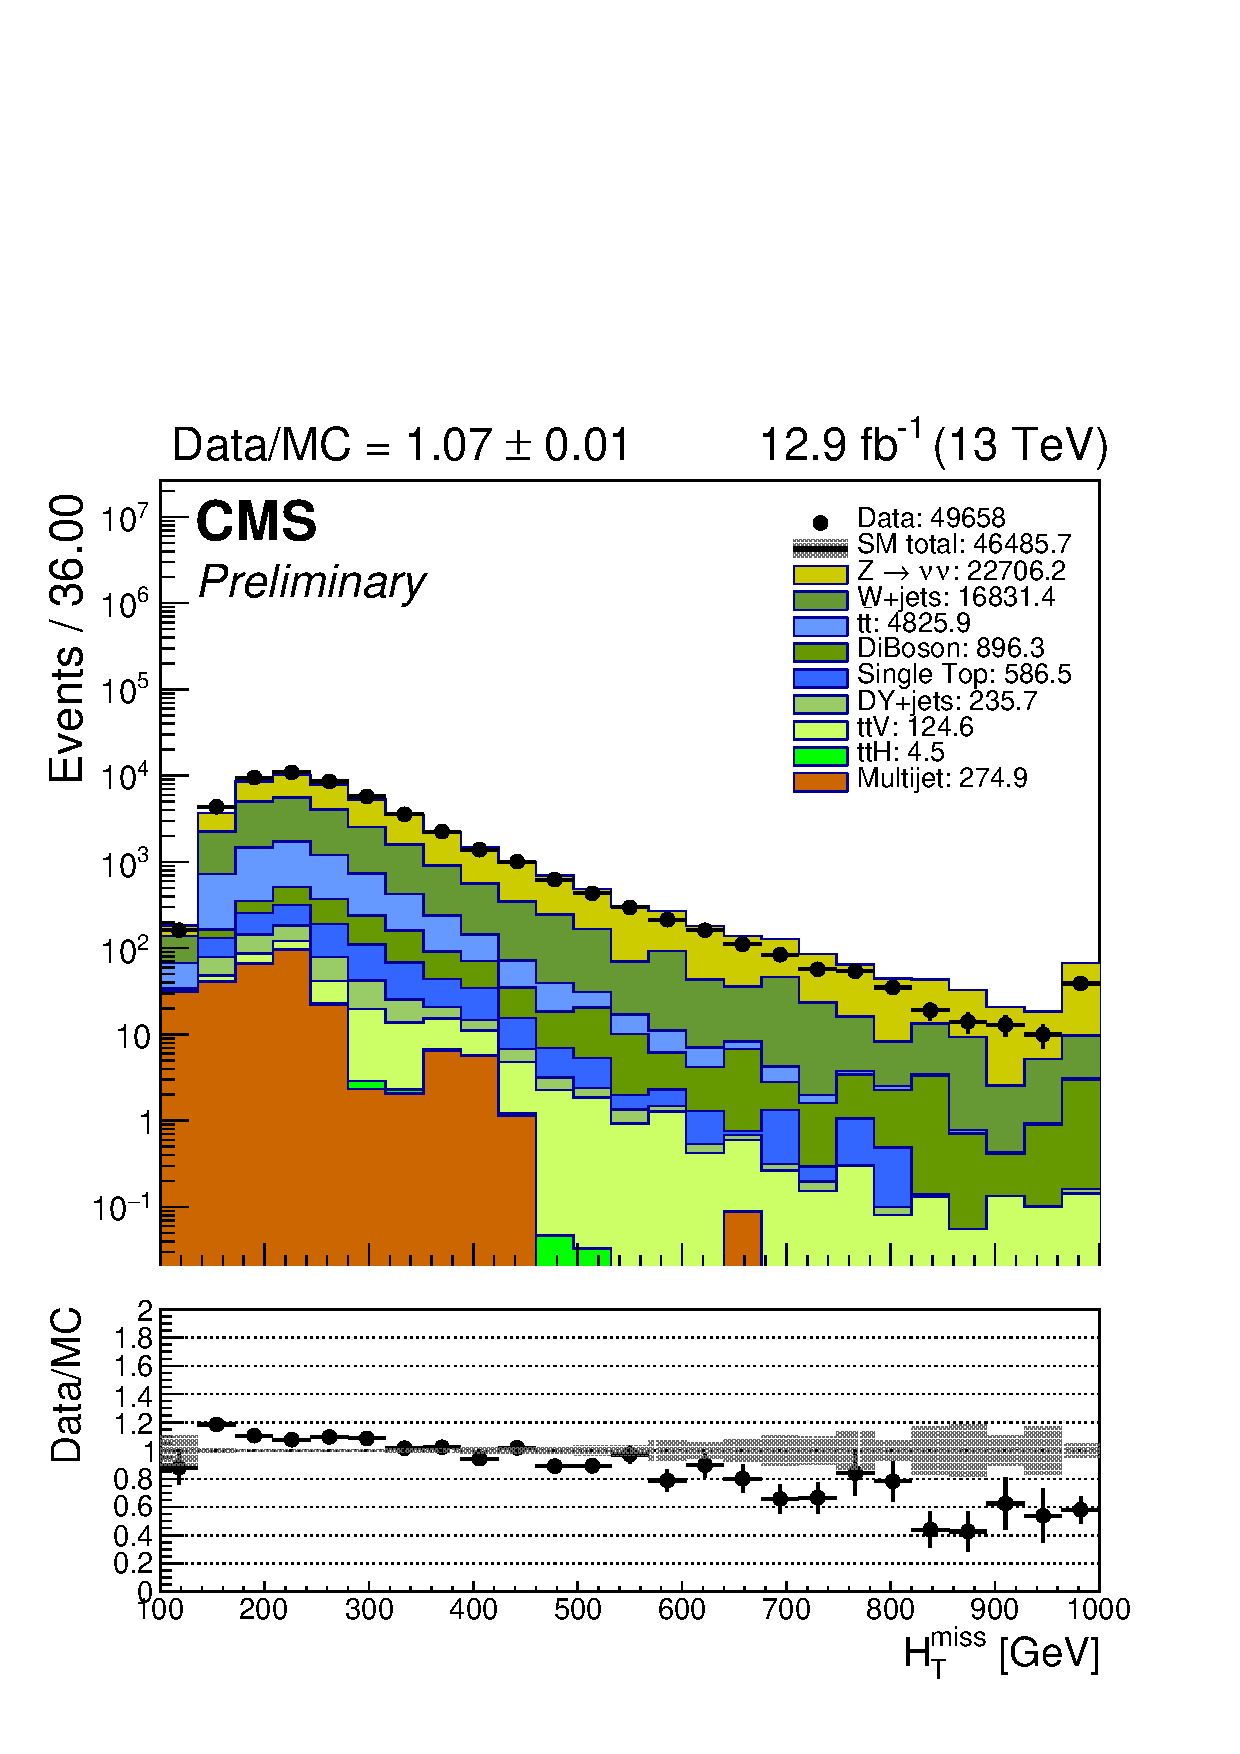
\includegraphics[width=0.5\textwidth]{figs/analysis/distributions/Signal/mht40_pt_sym.pdf}} ~~
        \subfloat {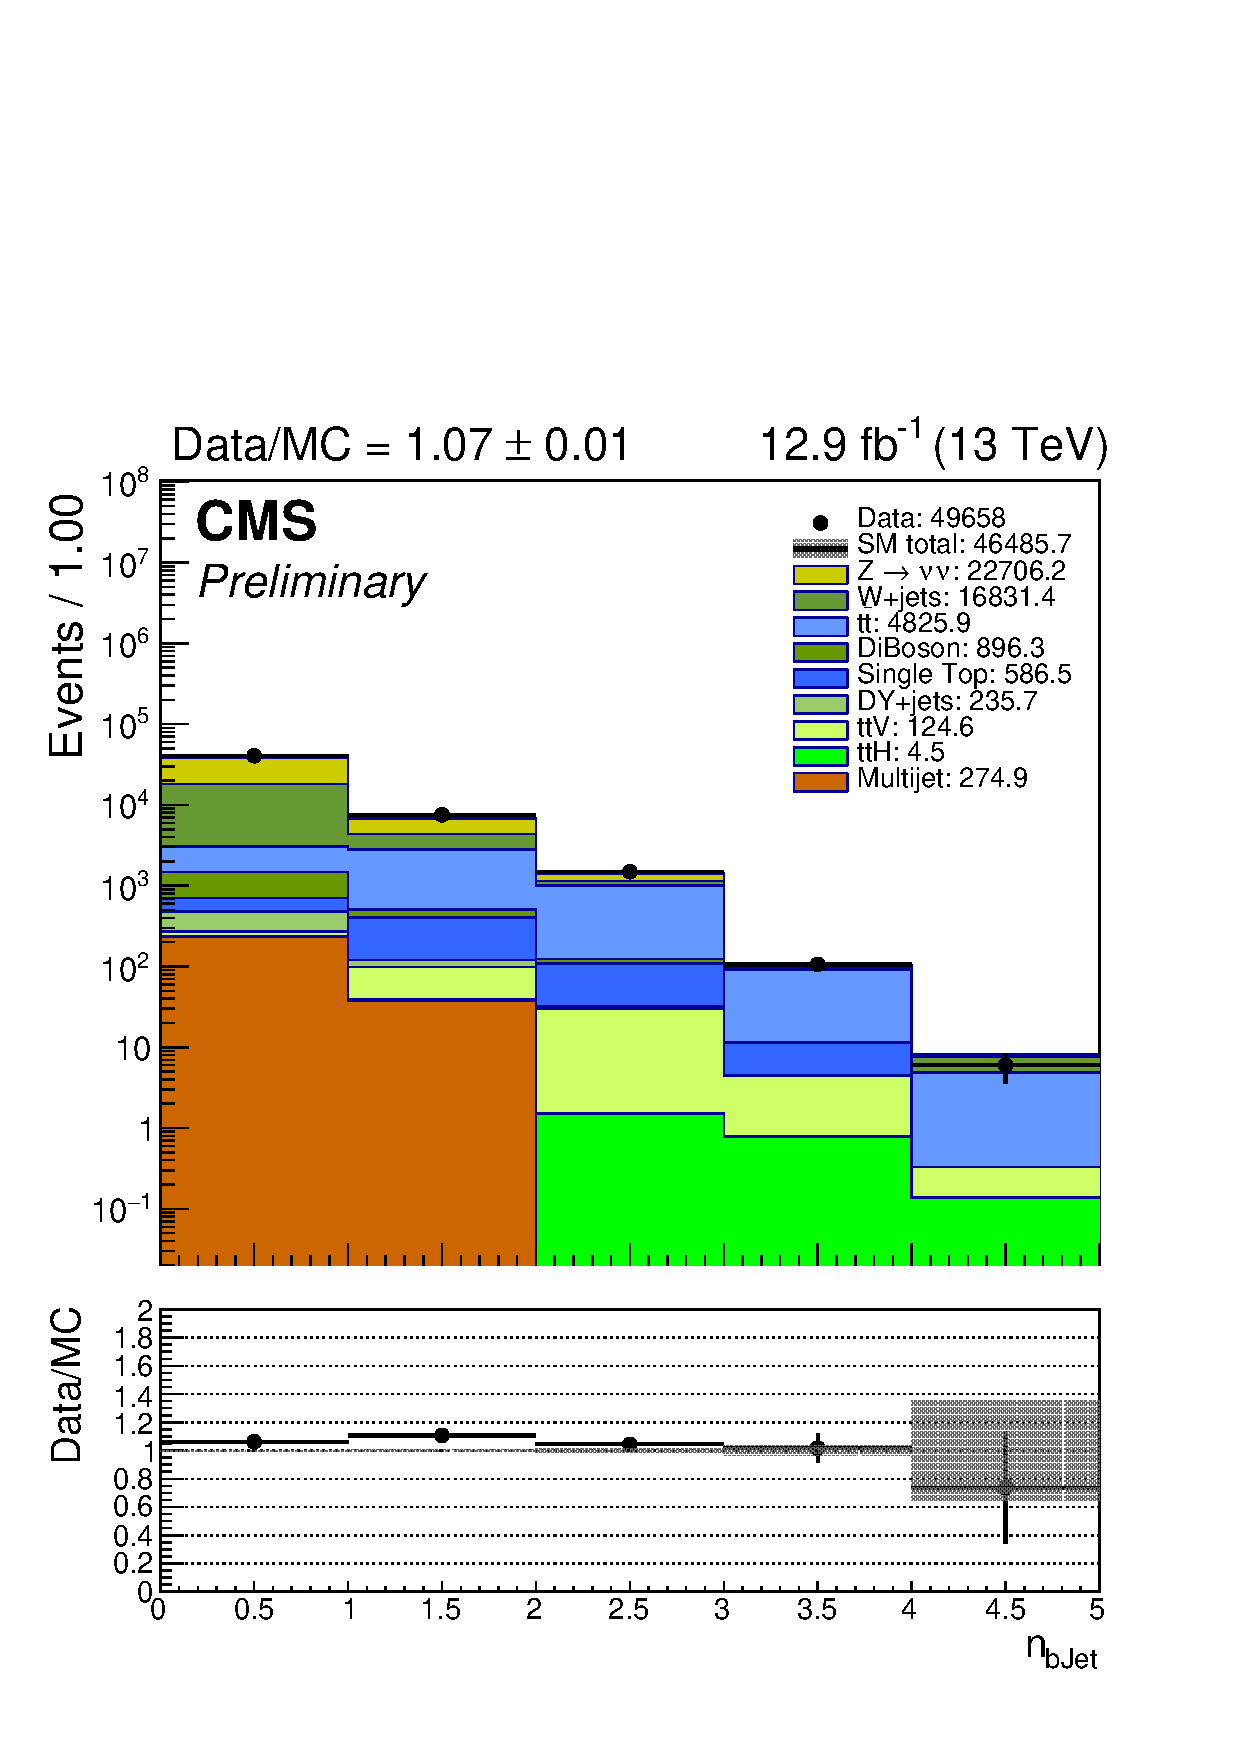
\includegraphics[width=0.5\textwidth]{figs/analysis/distributions/Signal/nBJet40_sym.pdf}} \\
        \caption{Key analysis variables for hadronic signal region (symmetric \njet bins)}
        \label{fig:distribution_signal_sym}
    \end{center}
\end{figure}

\clearpage
\begin{figure}
    \begin{center}
        \subfloat {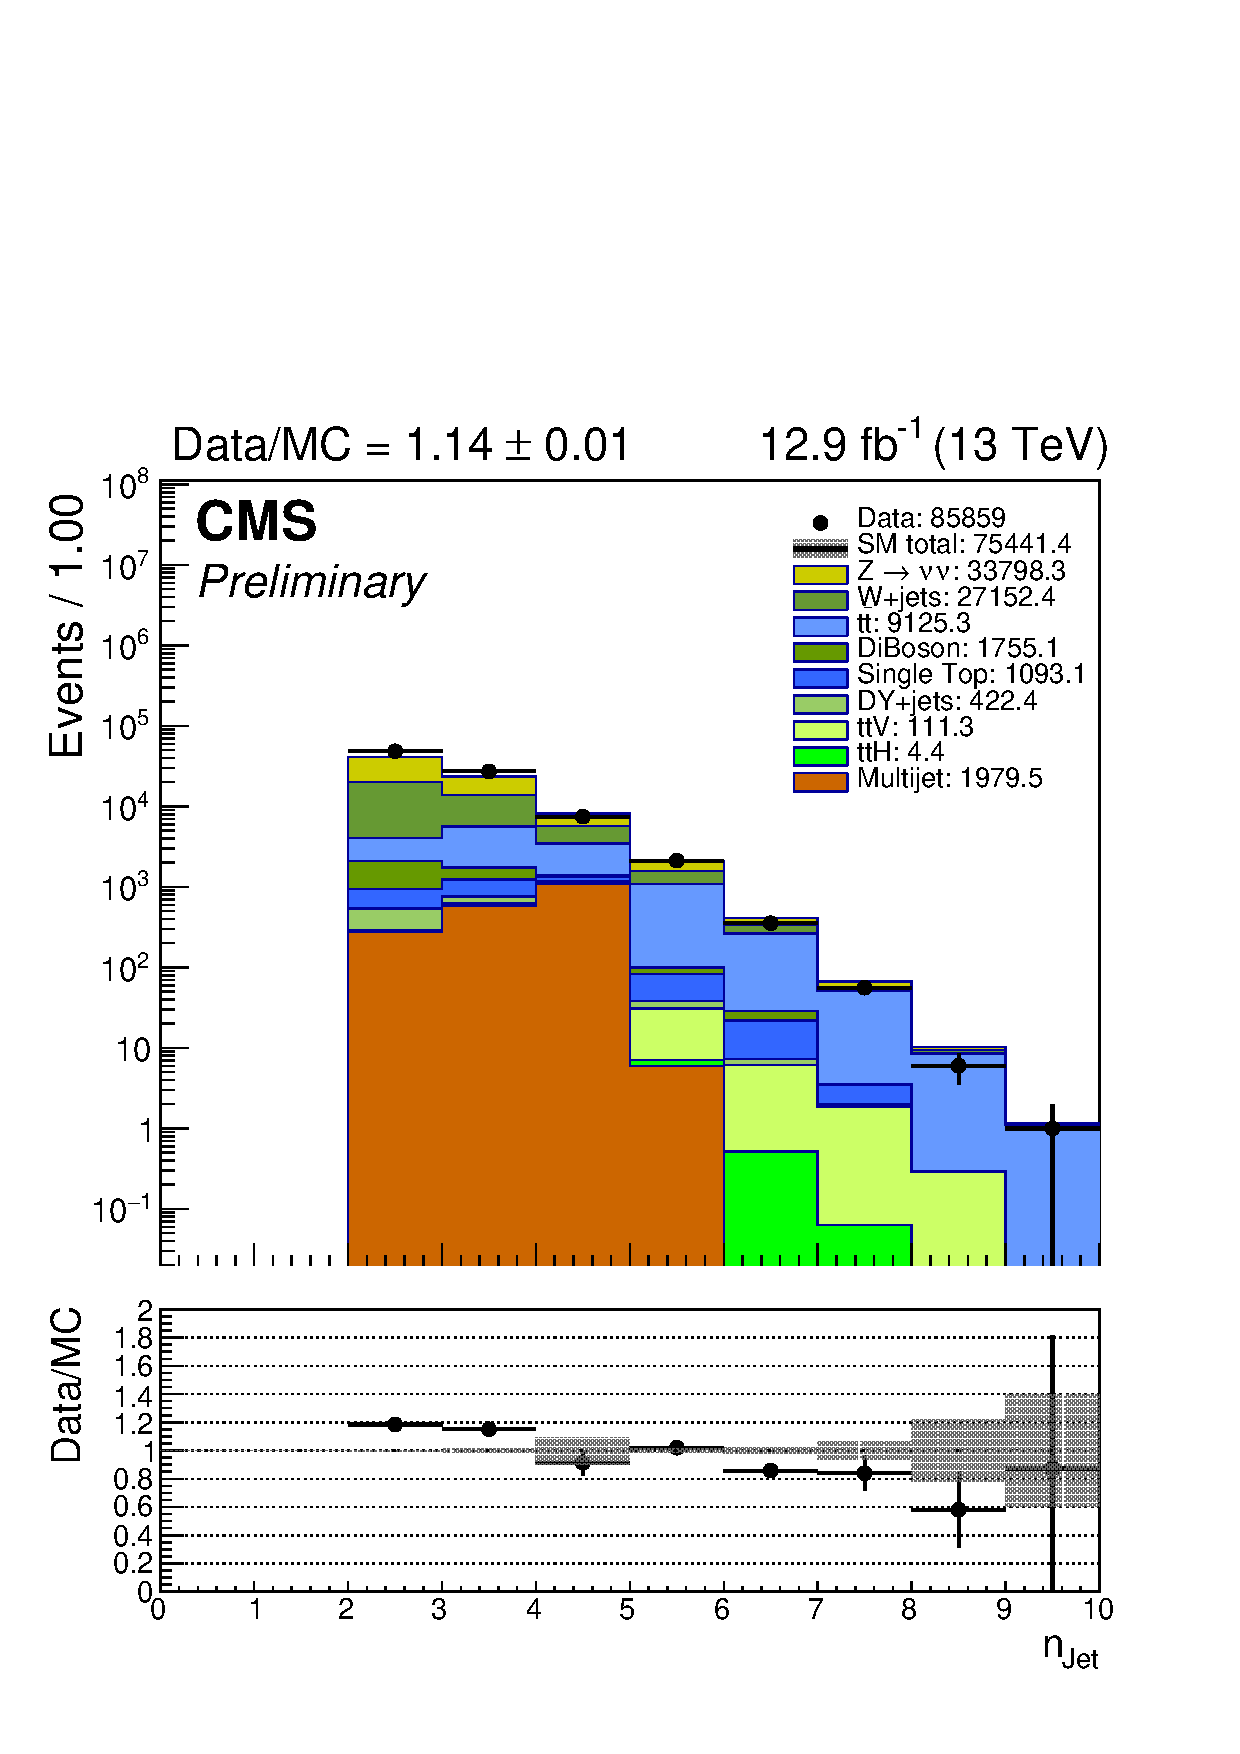
\includegraphics[width=0.5\textwidth]{figs/analysis/distributions/Signal/nJet40_asym.pdf}} ~~
        \subfloat {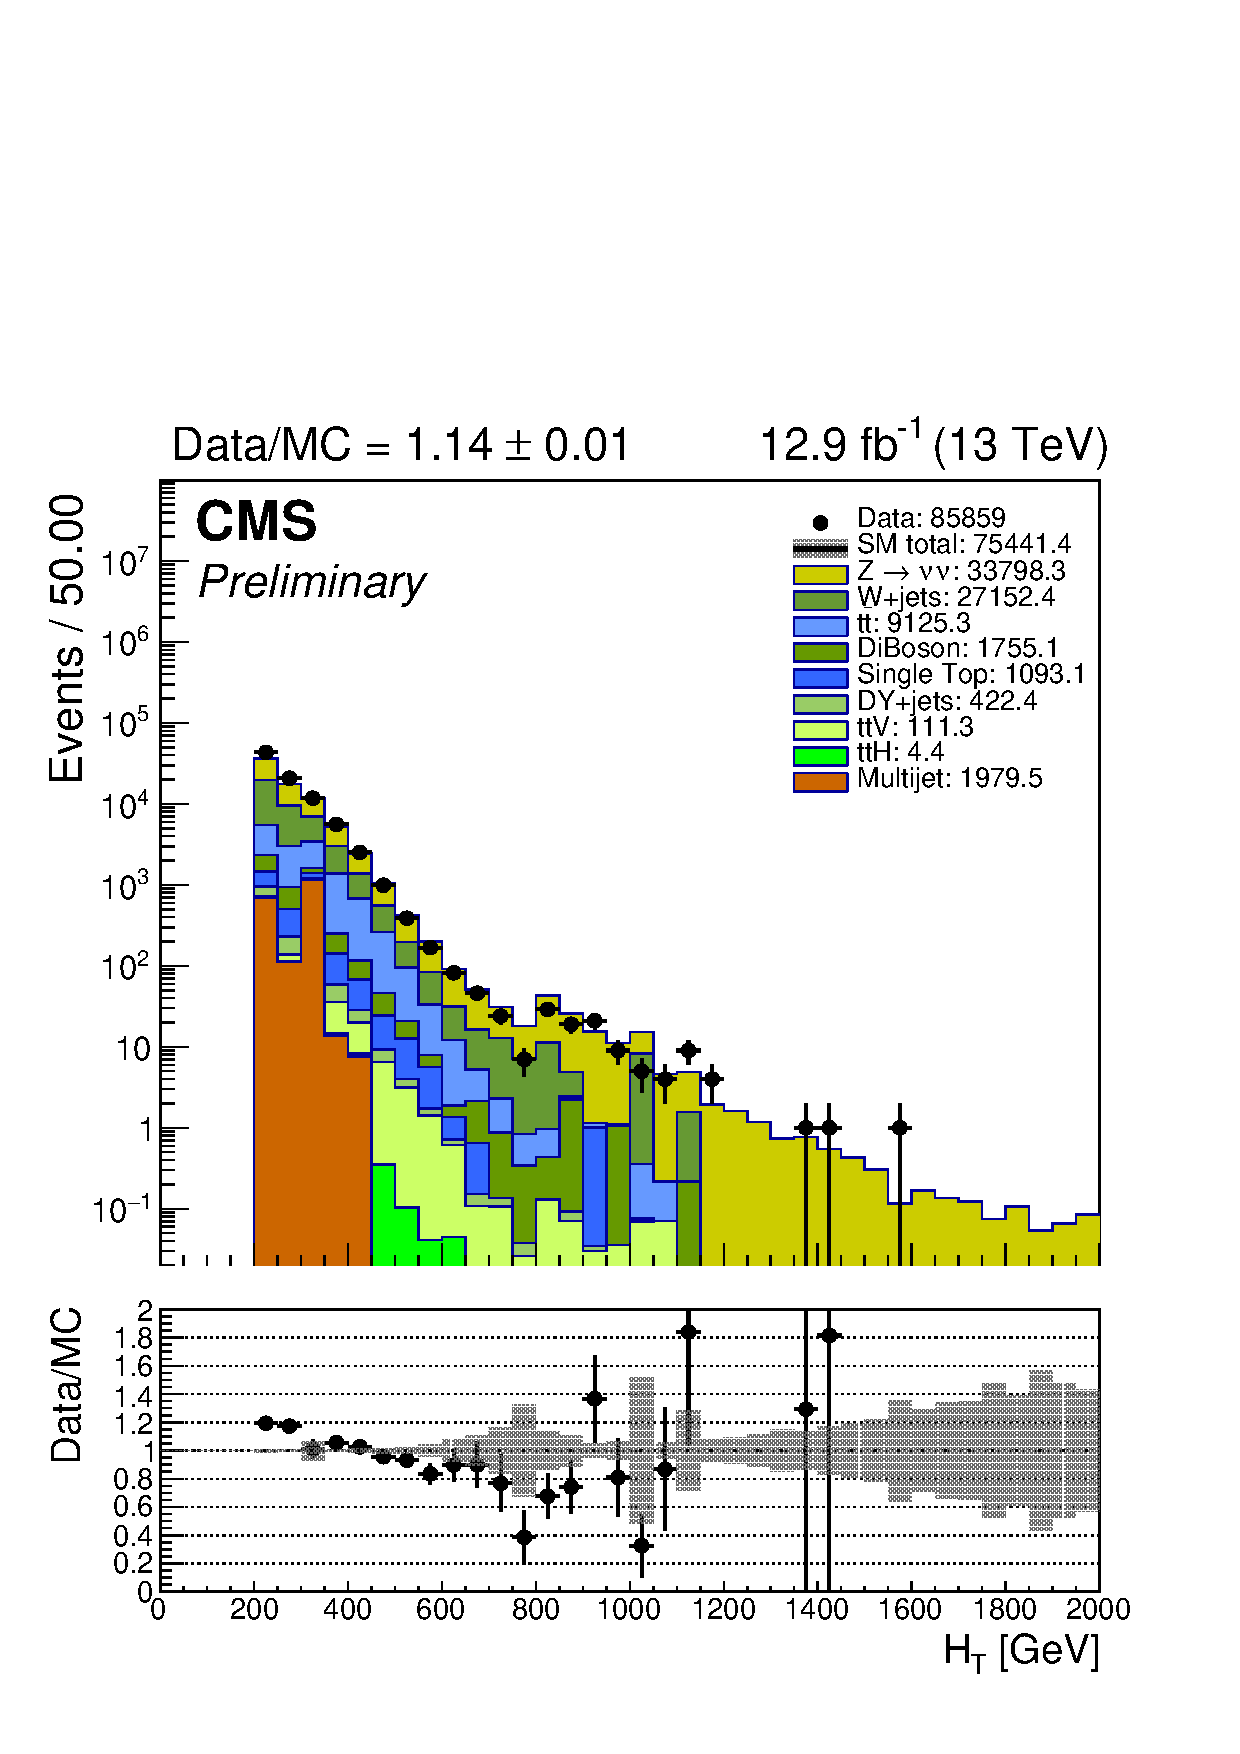
\includegraphics[width=0.5\textwidth]{figs/analysis/distributions/Signal/ht40_asym.pdf}} \\
        \subfloat {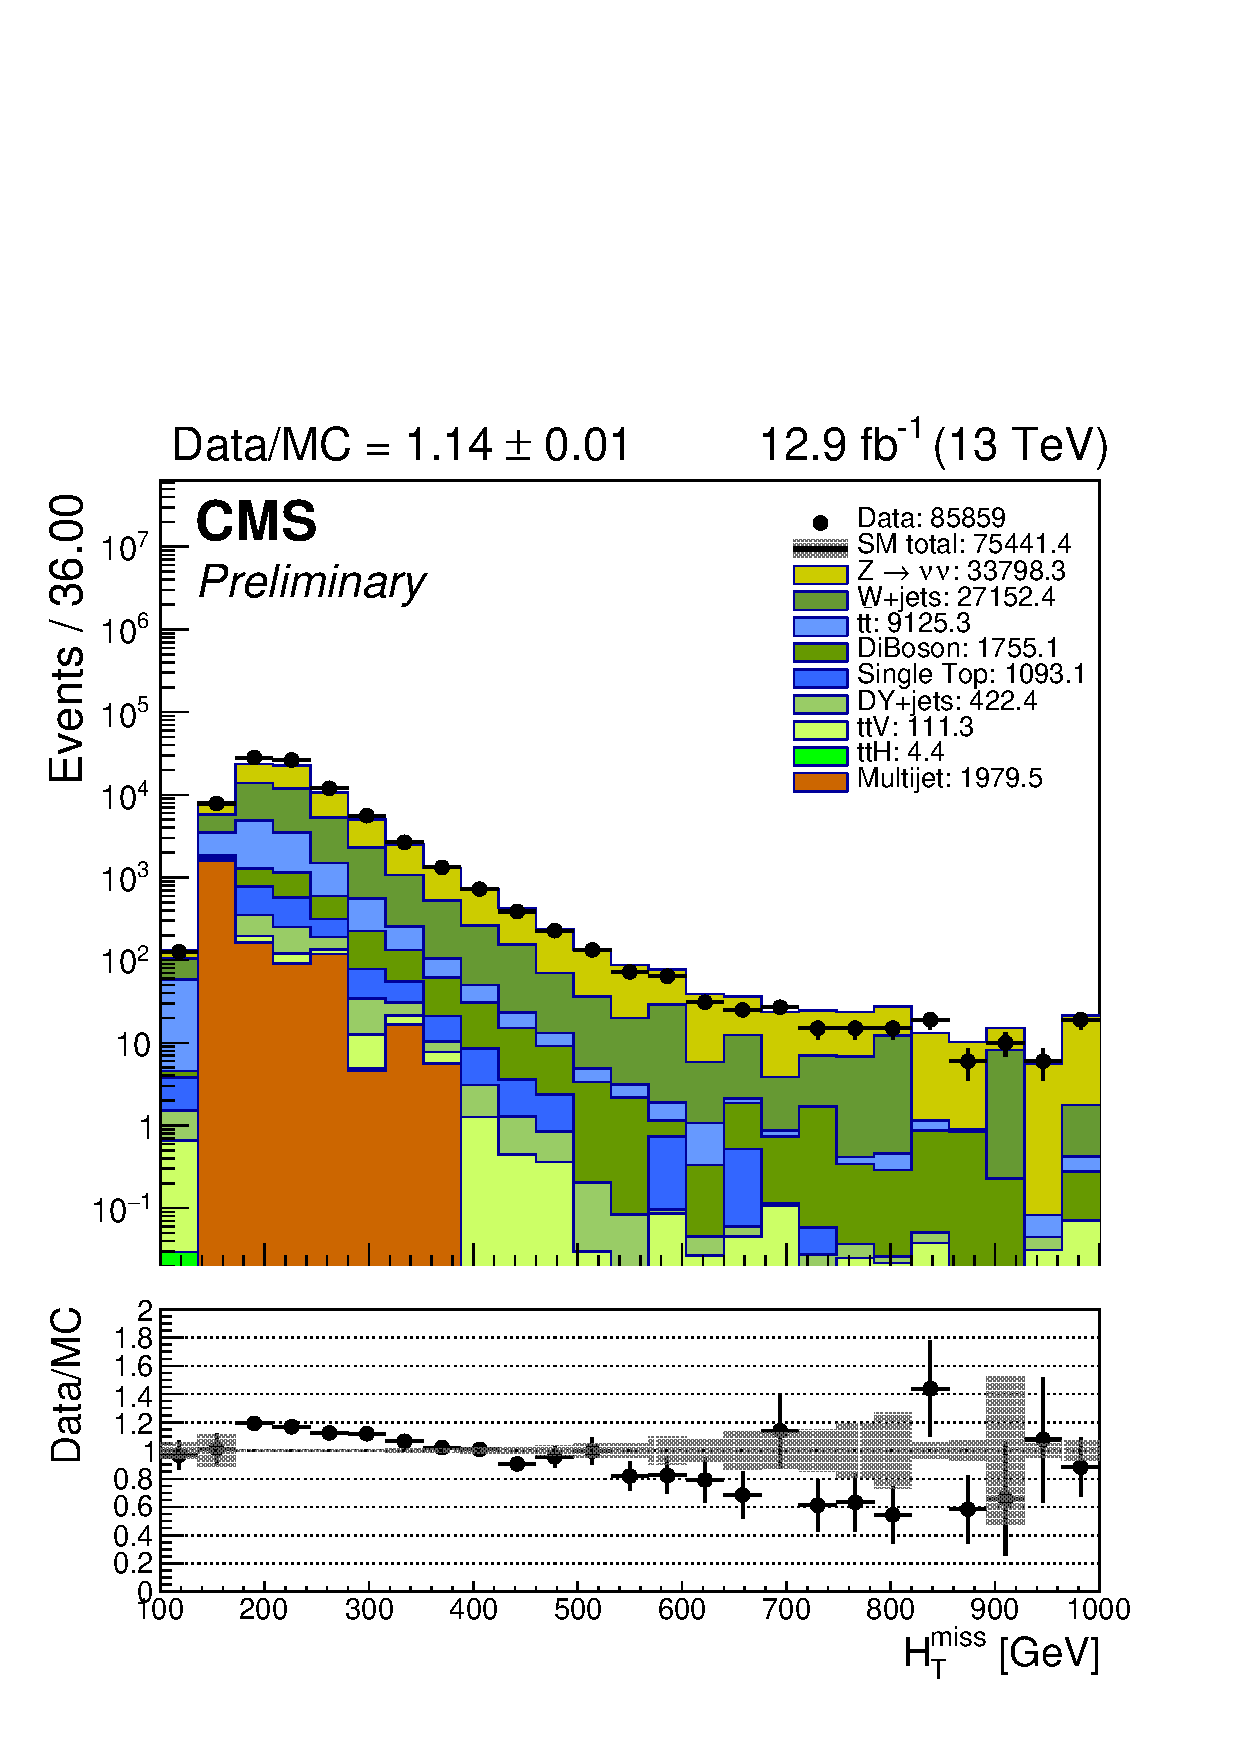
\includegraphics[width=0.5\textwidth]{figs/analysis/distributions/Signal/mht40_pt_asym.pdf}} ~~
        \subfloat {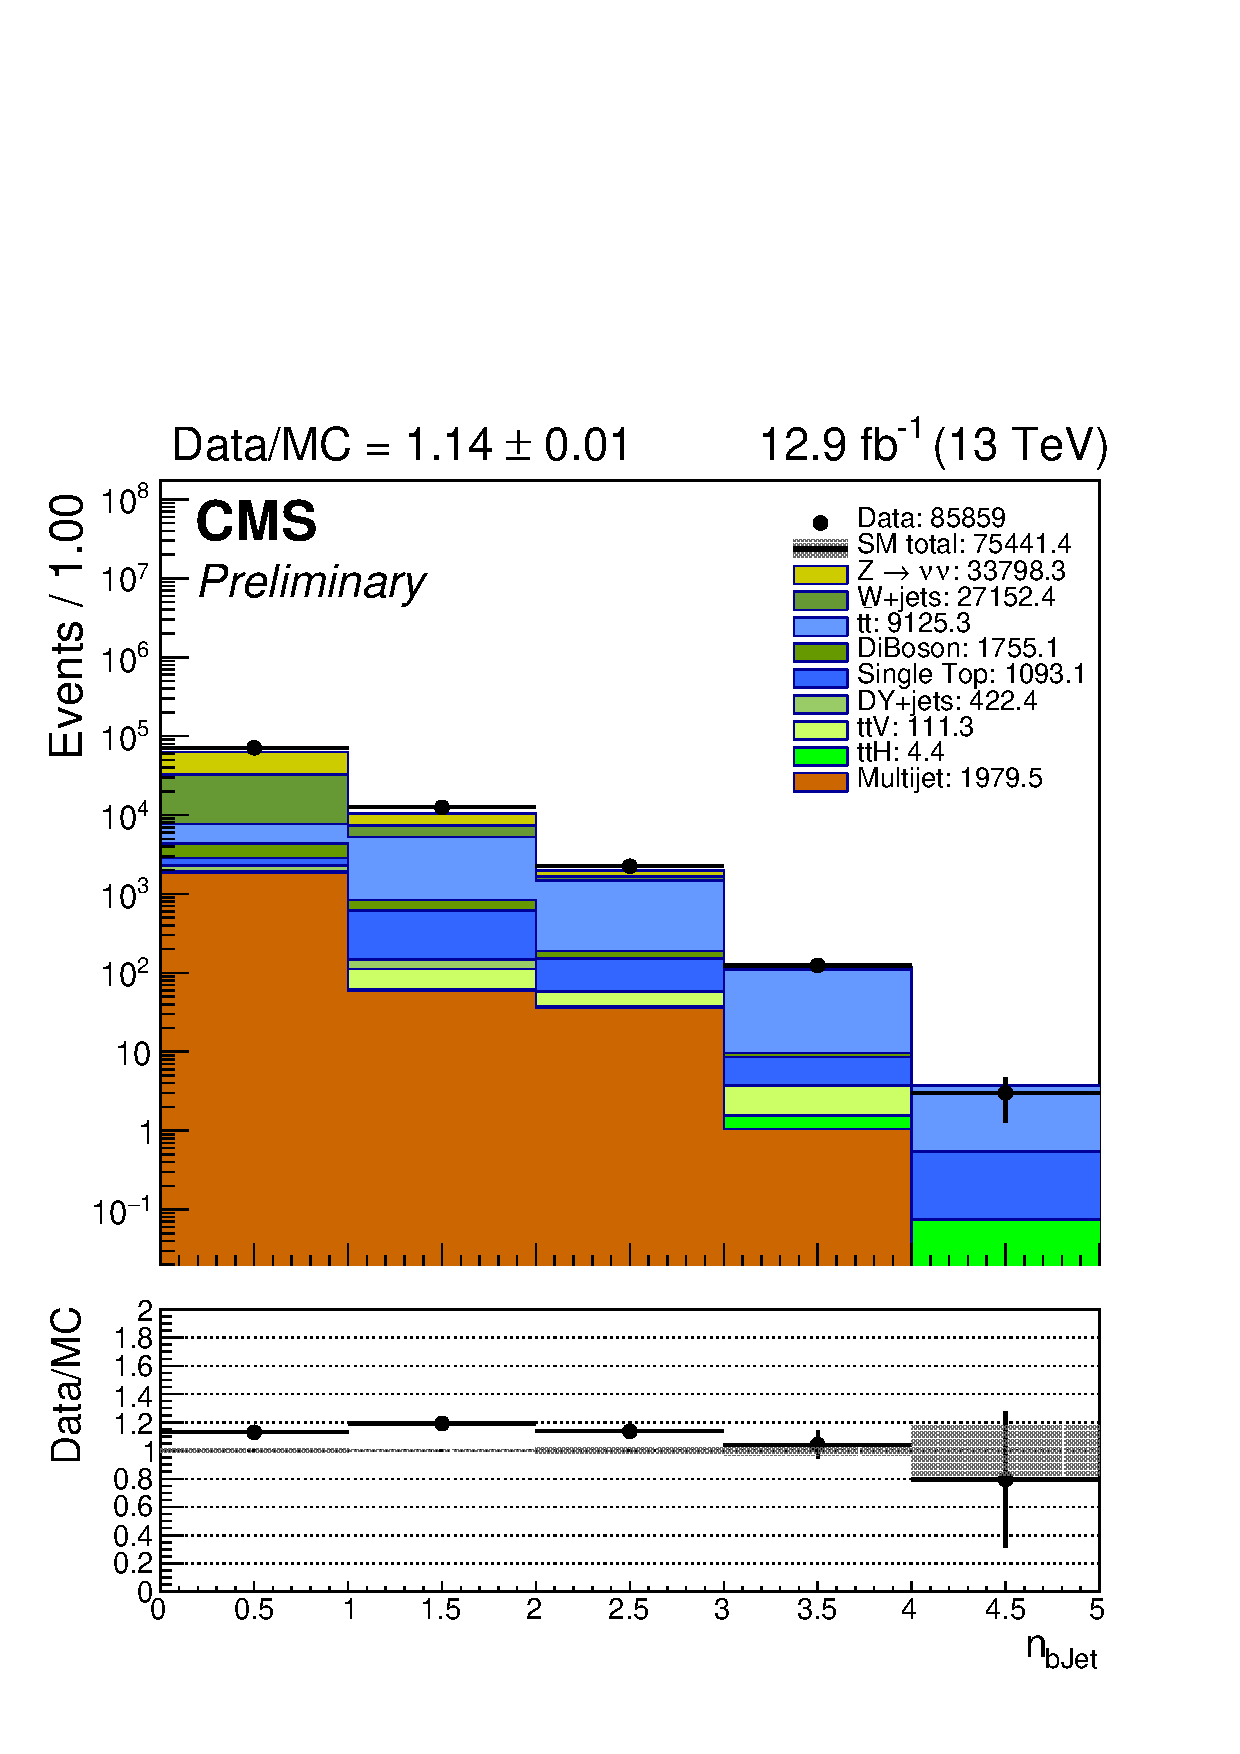
\includegraphics[width=0.5\textwidth]{figs/analysis/distributions/Signal/nBJet40_asym.pdf}} \\
        \caption{Key analysis variables for hadronic signal region (asymmetric \njet bins)}
        \label{fig:distribution_signal_asym}
    \end{center}
\end{figure}

\clearpage
\begin{figure}
    \begin{center}
        \subfloat {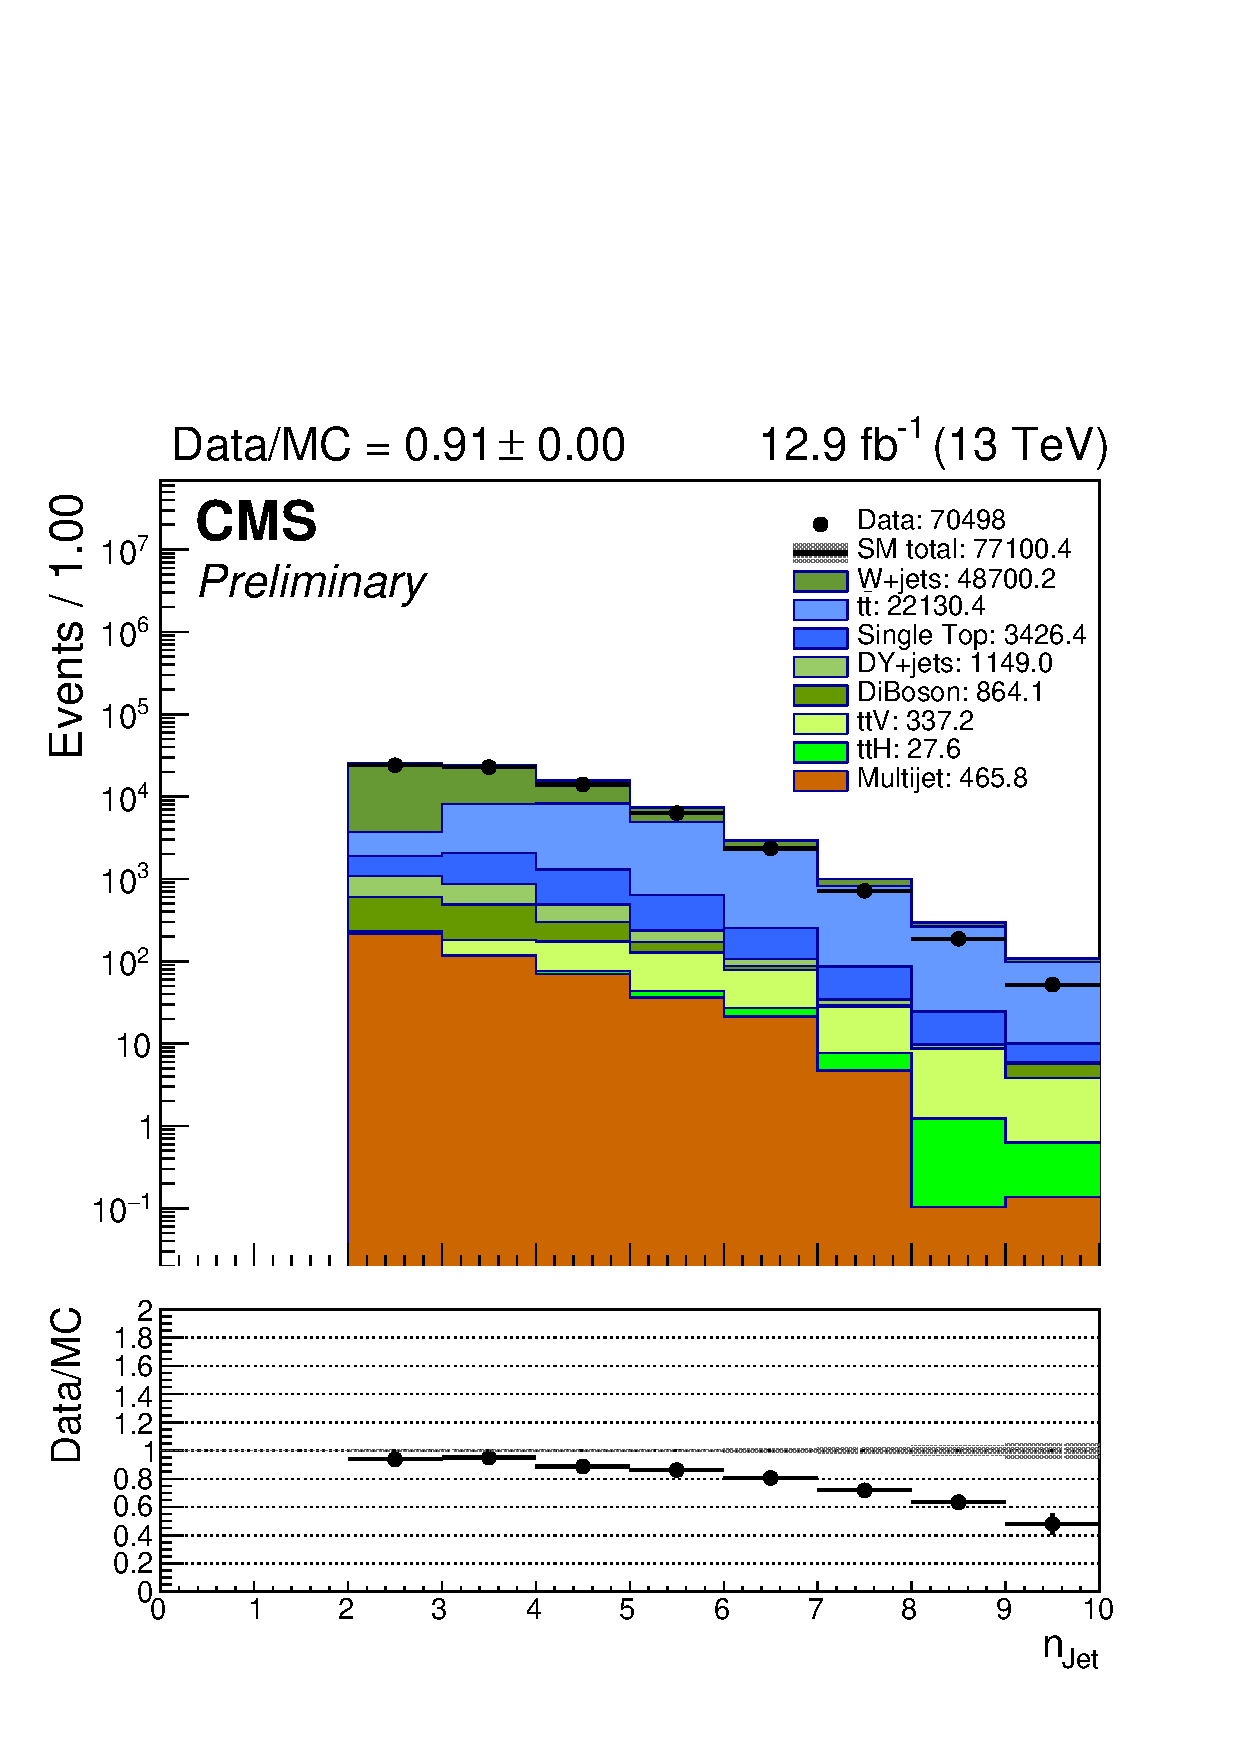
\includegraphics[width=0.5\textwidth]{figs/analysis/distributions/SingleMu/nJet40_sym.pdf}} ~~
        \subfloat {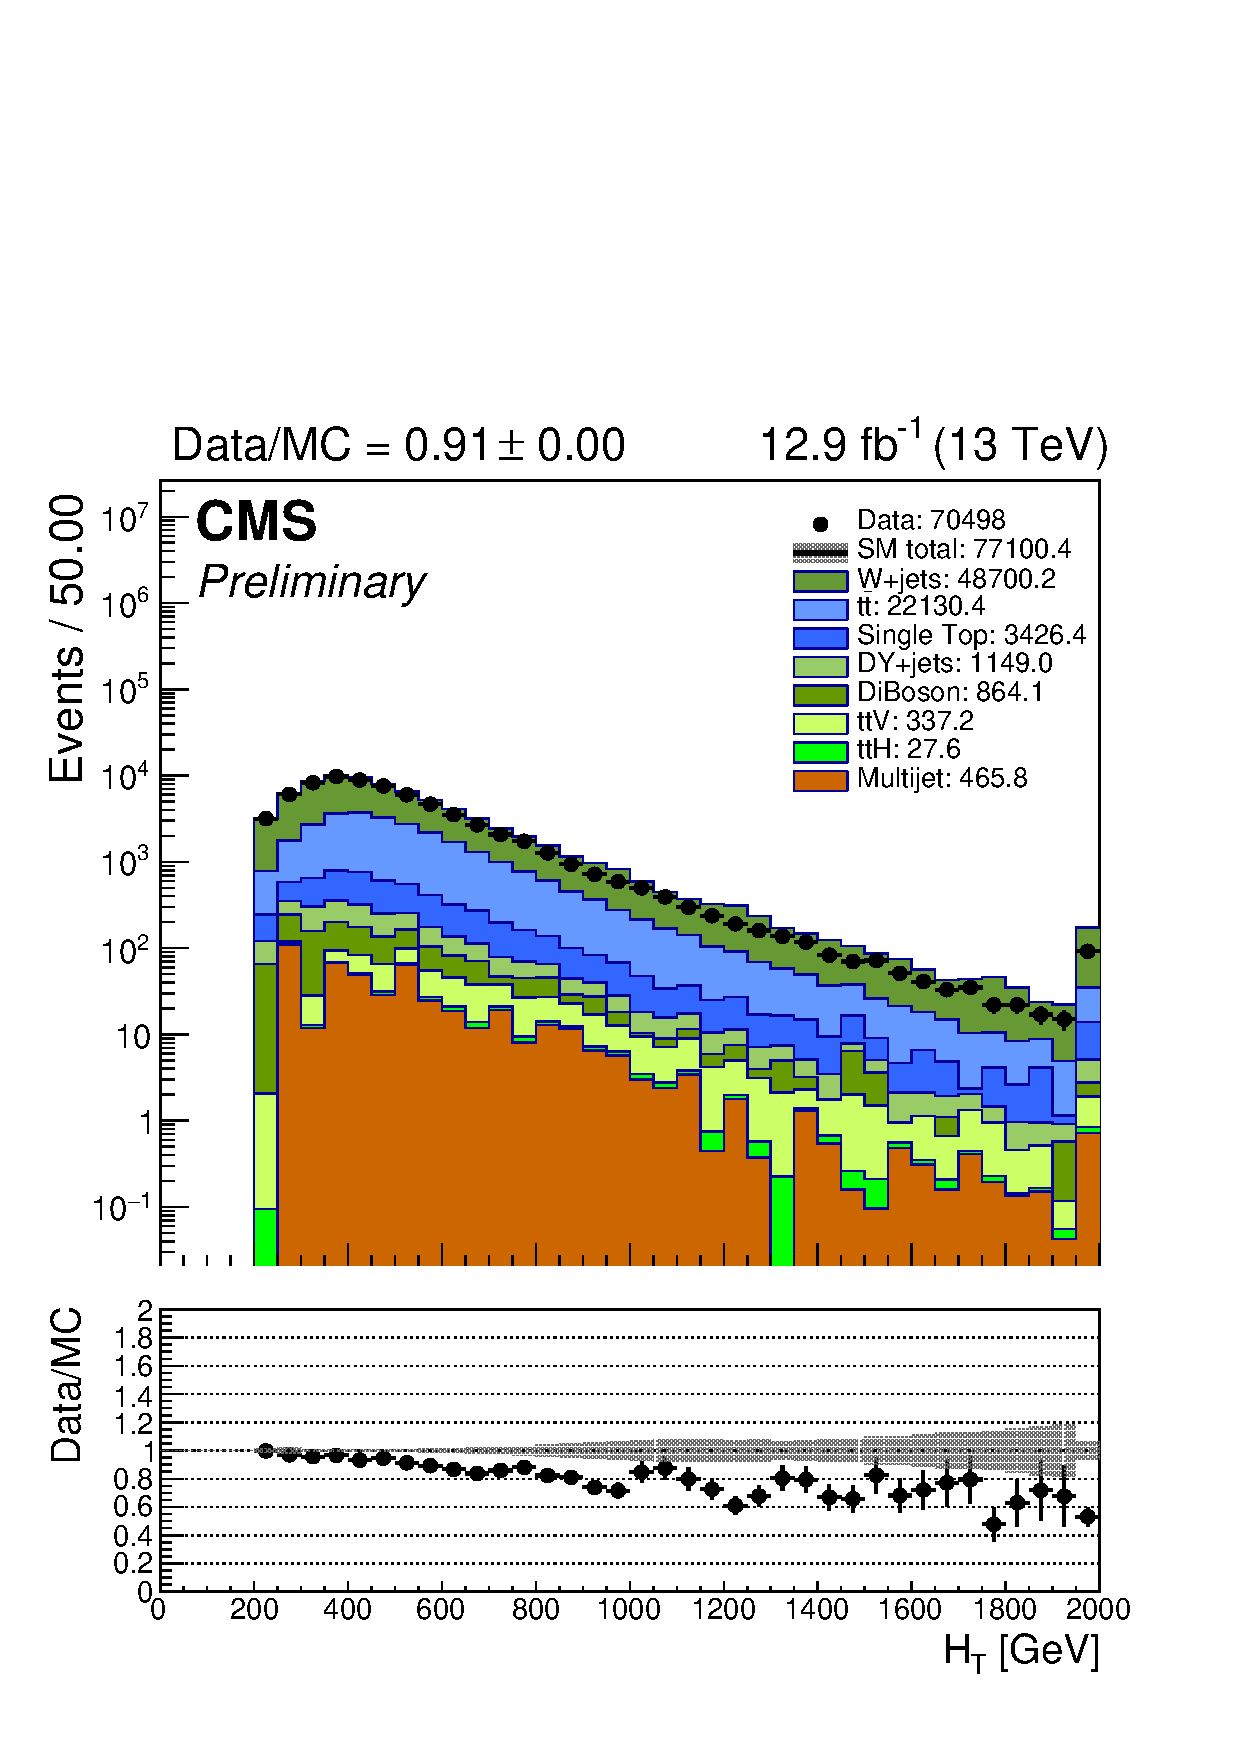
\includegraphics[width=0.5\textwidth]{figs/analysis/distributions/SingleMu/ht40_sym.pdf}} \\
        \subfloat {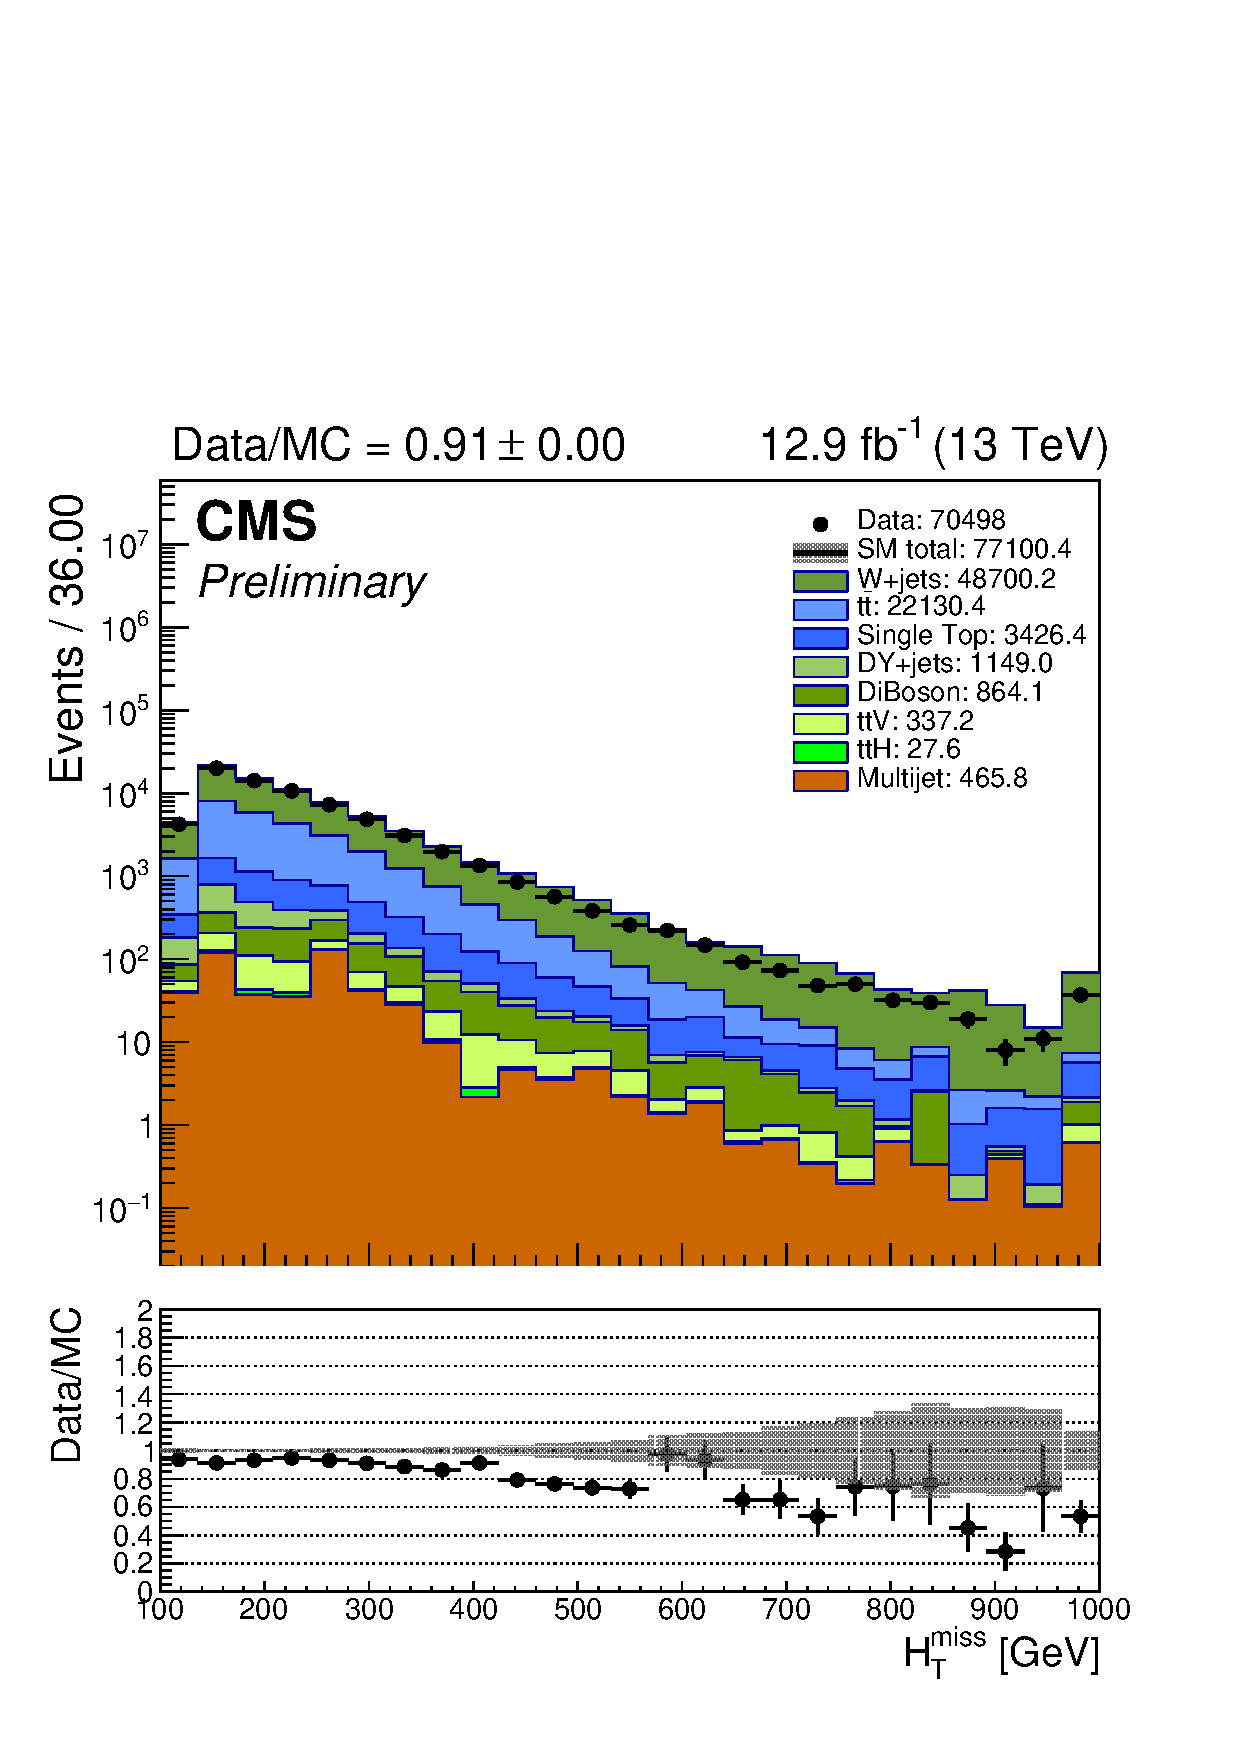
\includegraphics[width=0.5\textwidth]{figs/analysis/distributions/SingleMu/mht40_pt_sym.pdf}} ~~
        \subfloat {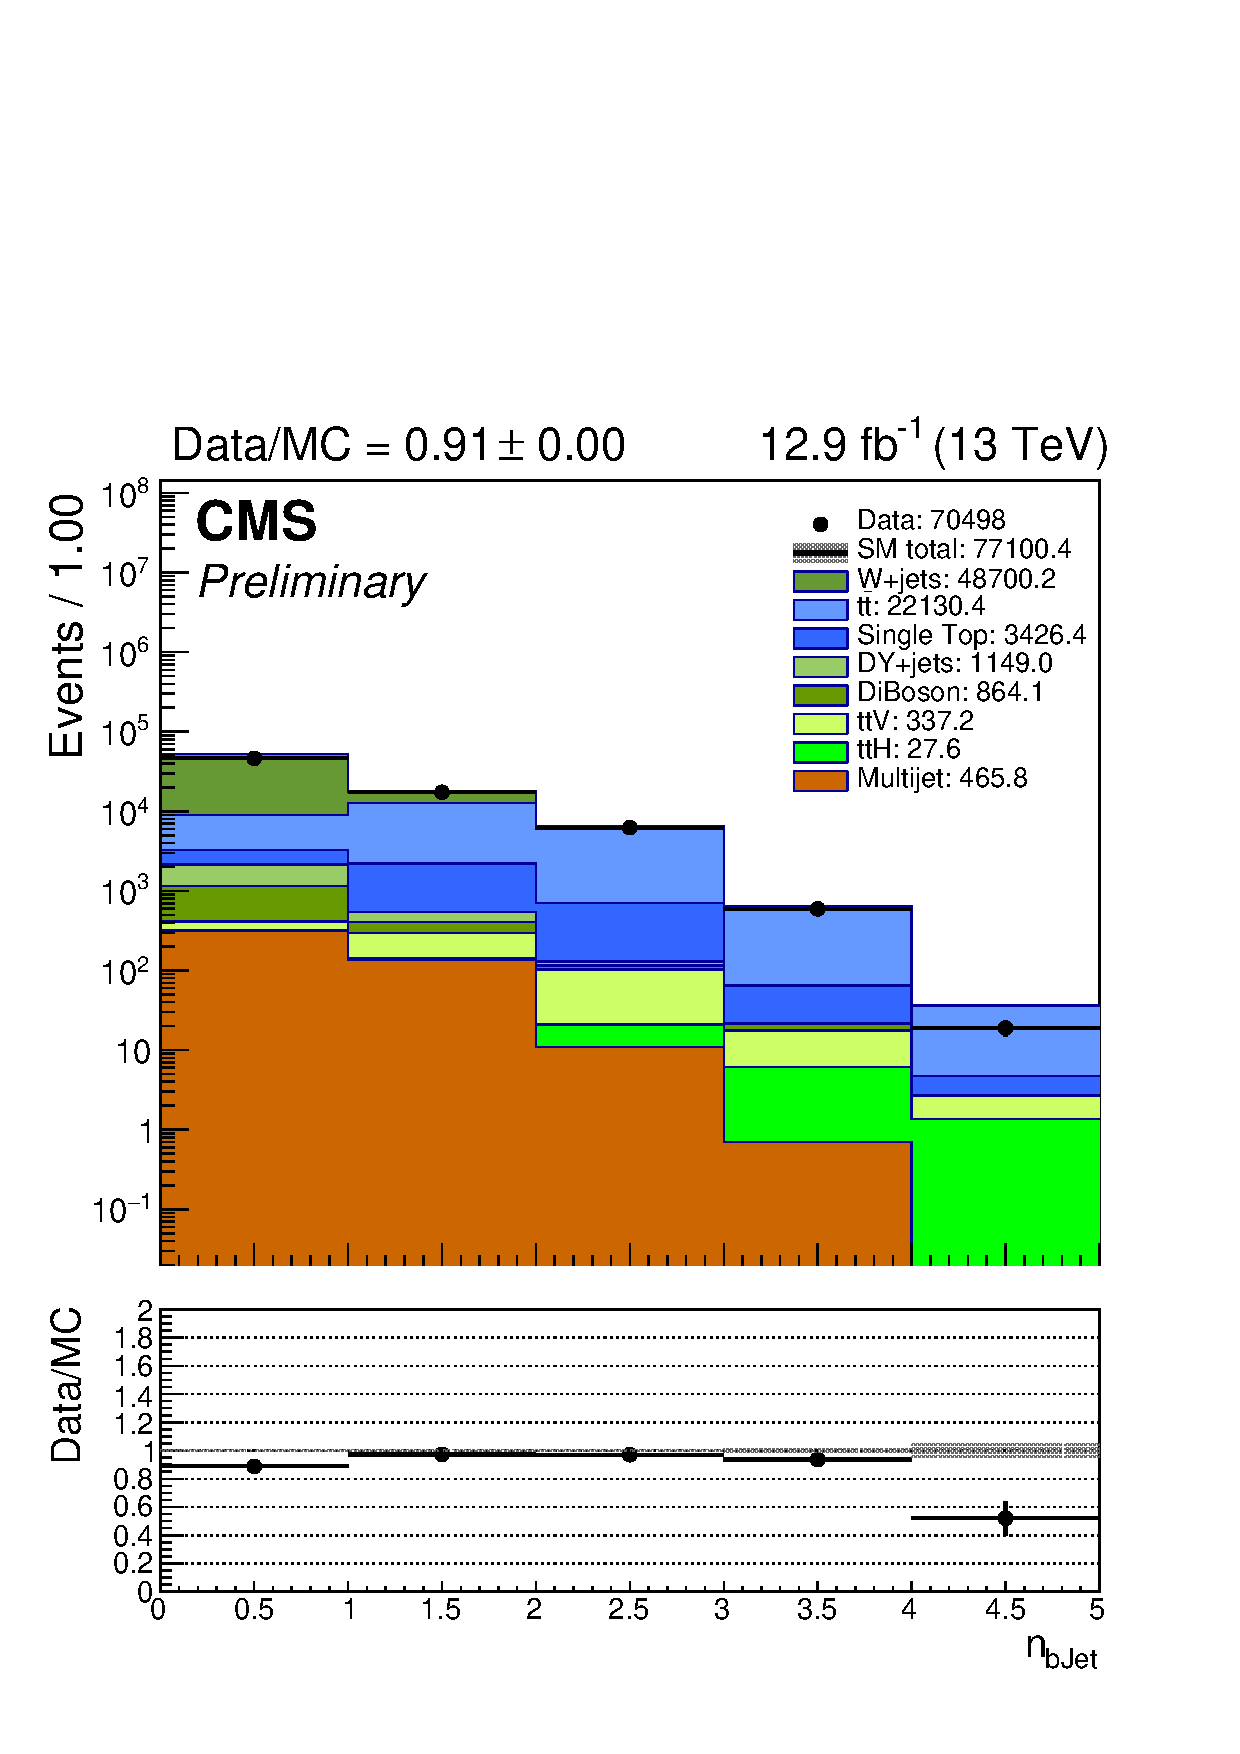
\includegraphics[width=0.5\textwidth]{figs/analysis/distributions/SingleMu/nBJet40_sym.pdf}} \\
        \caption{Key analysis variables for single muon control region (symmetric \njet bins)}
        \label{fig:distribution_singlemu_sym}
    \end{center}
\end{figure}

\clearpage
\begin{figure}
    \begin{center}
        \subfloat {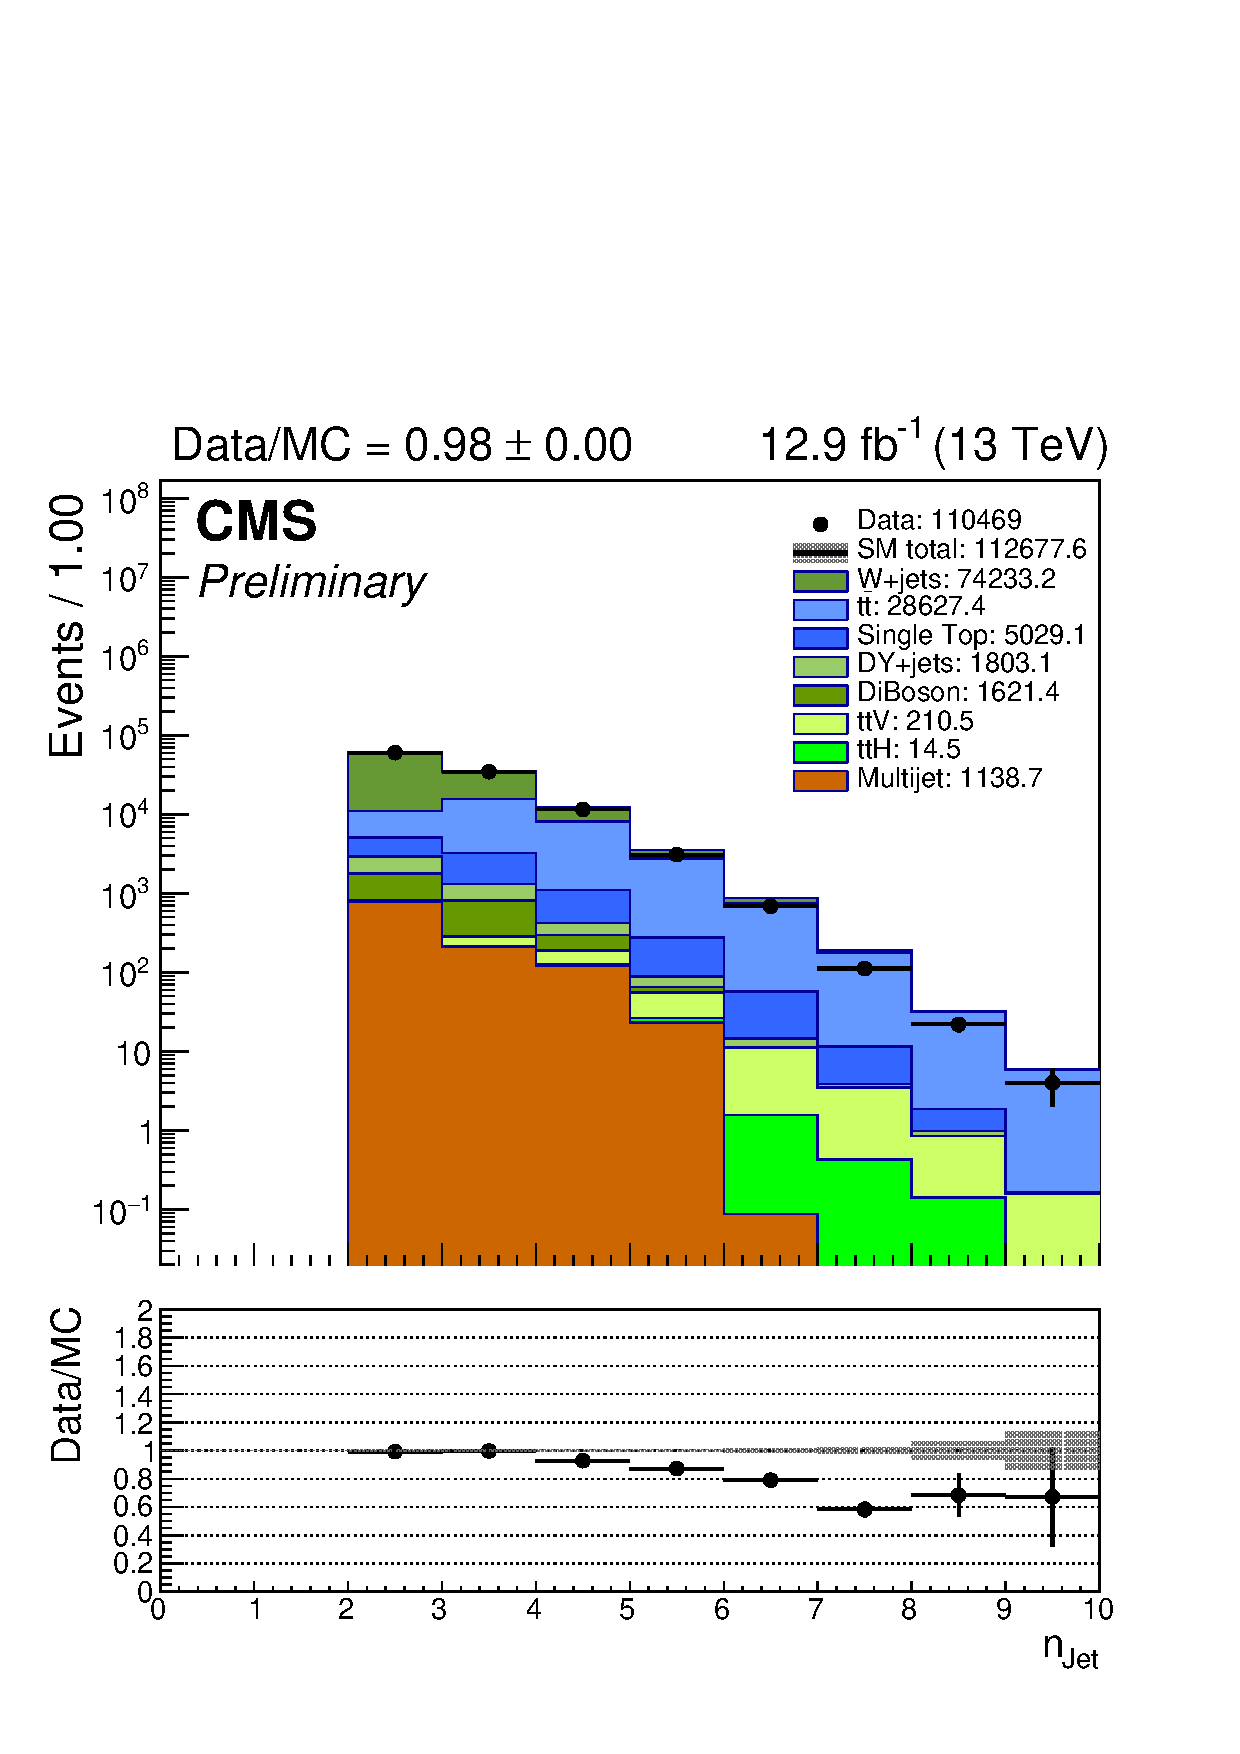
\includegraphics[width=0.5\textwidth]{figs/analysis/distributions/SingleMu/nJet40_asym.pdf}} ~~
        \subfloat {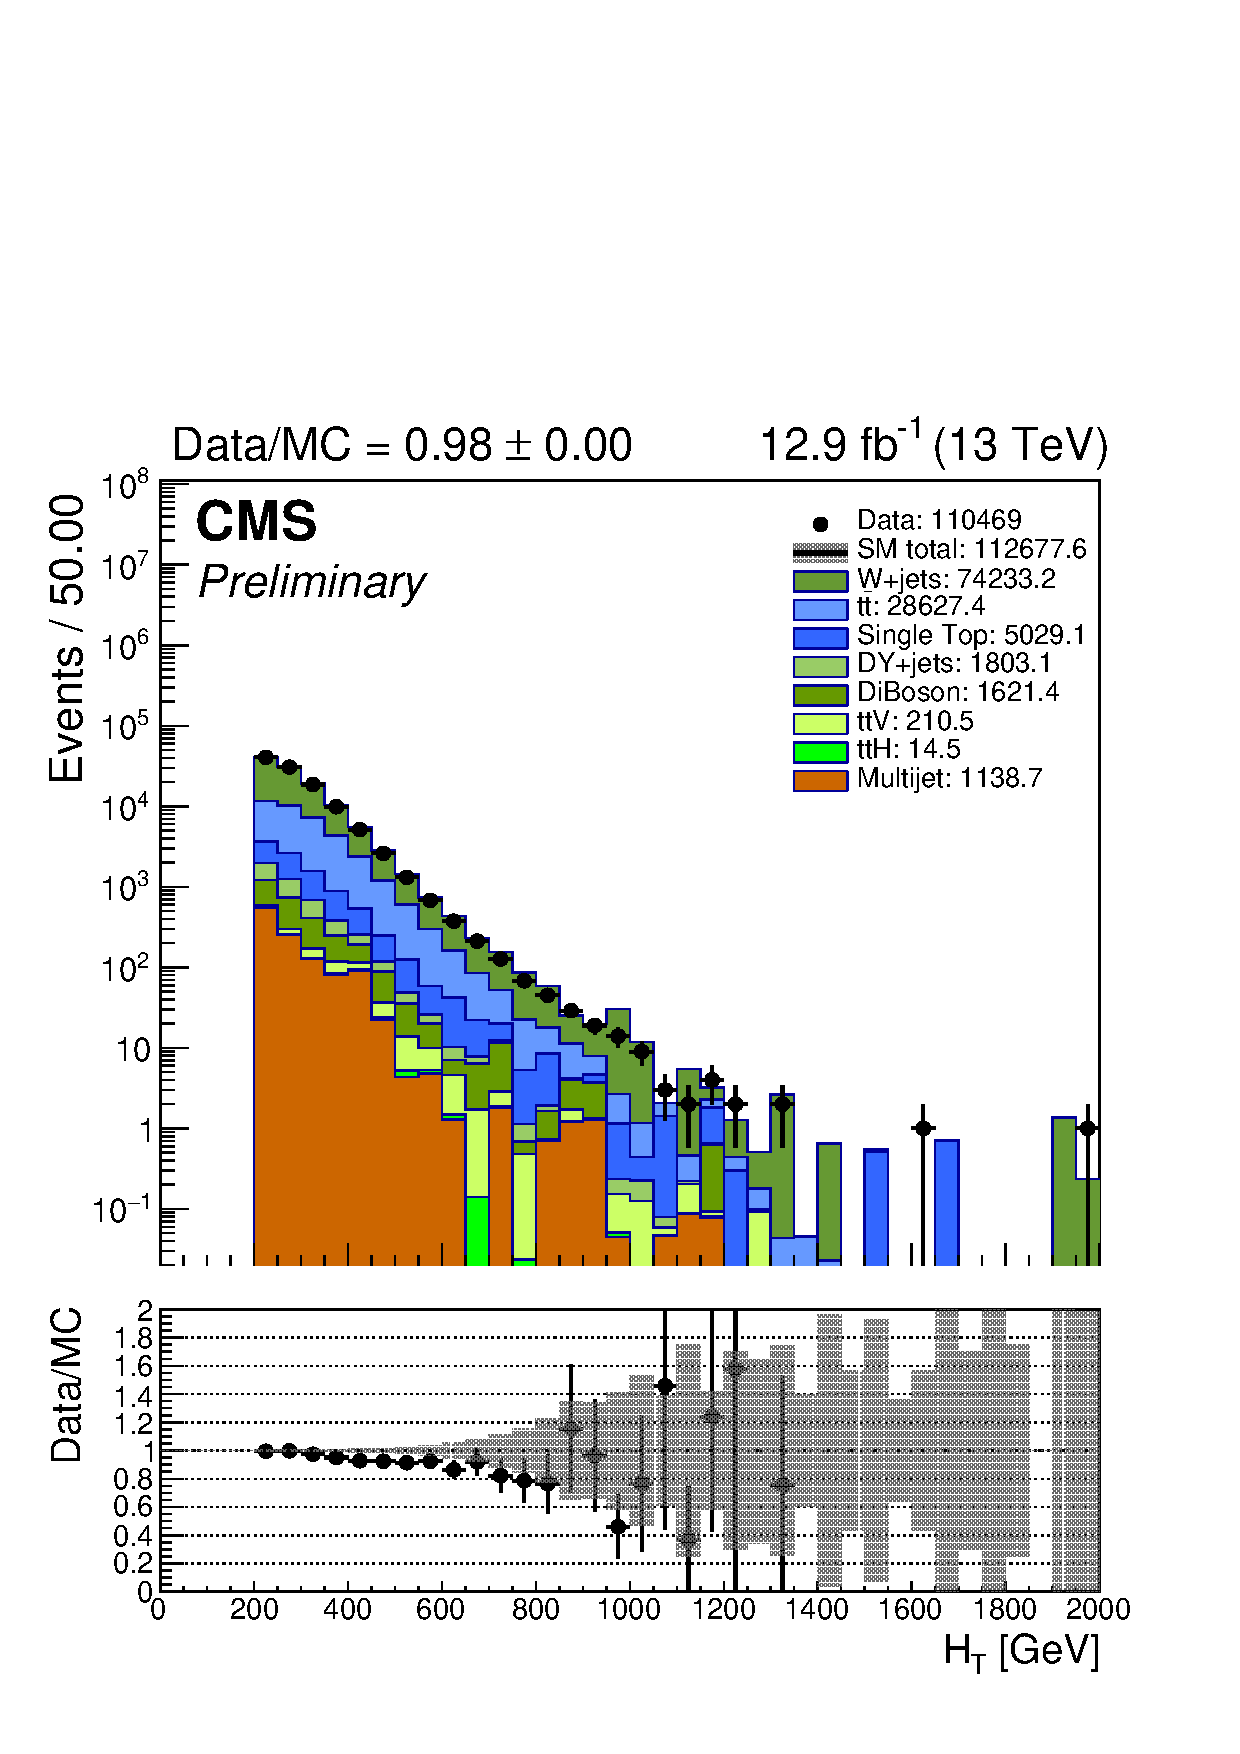
\includegraphics[width=0.5\textwidth]{figs/analysis/distributions/SingleMu/ht40_asym.pdf}} \\
        \subfloat {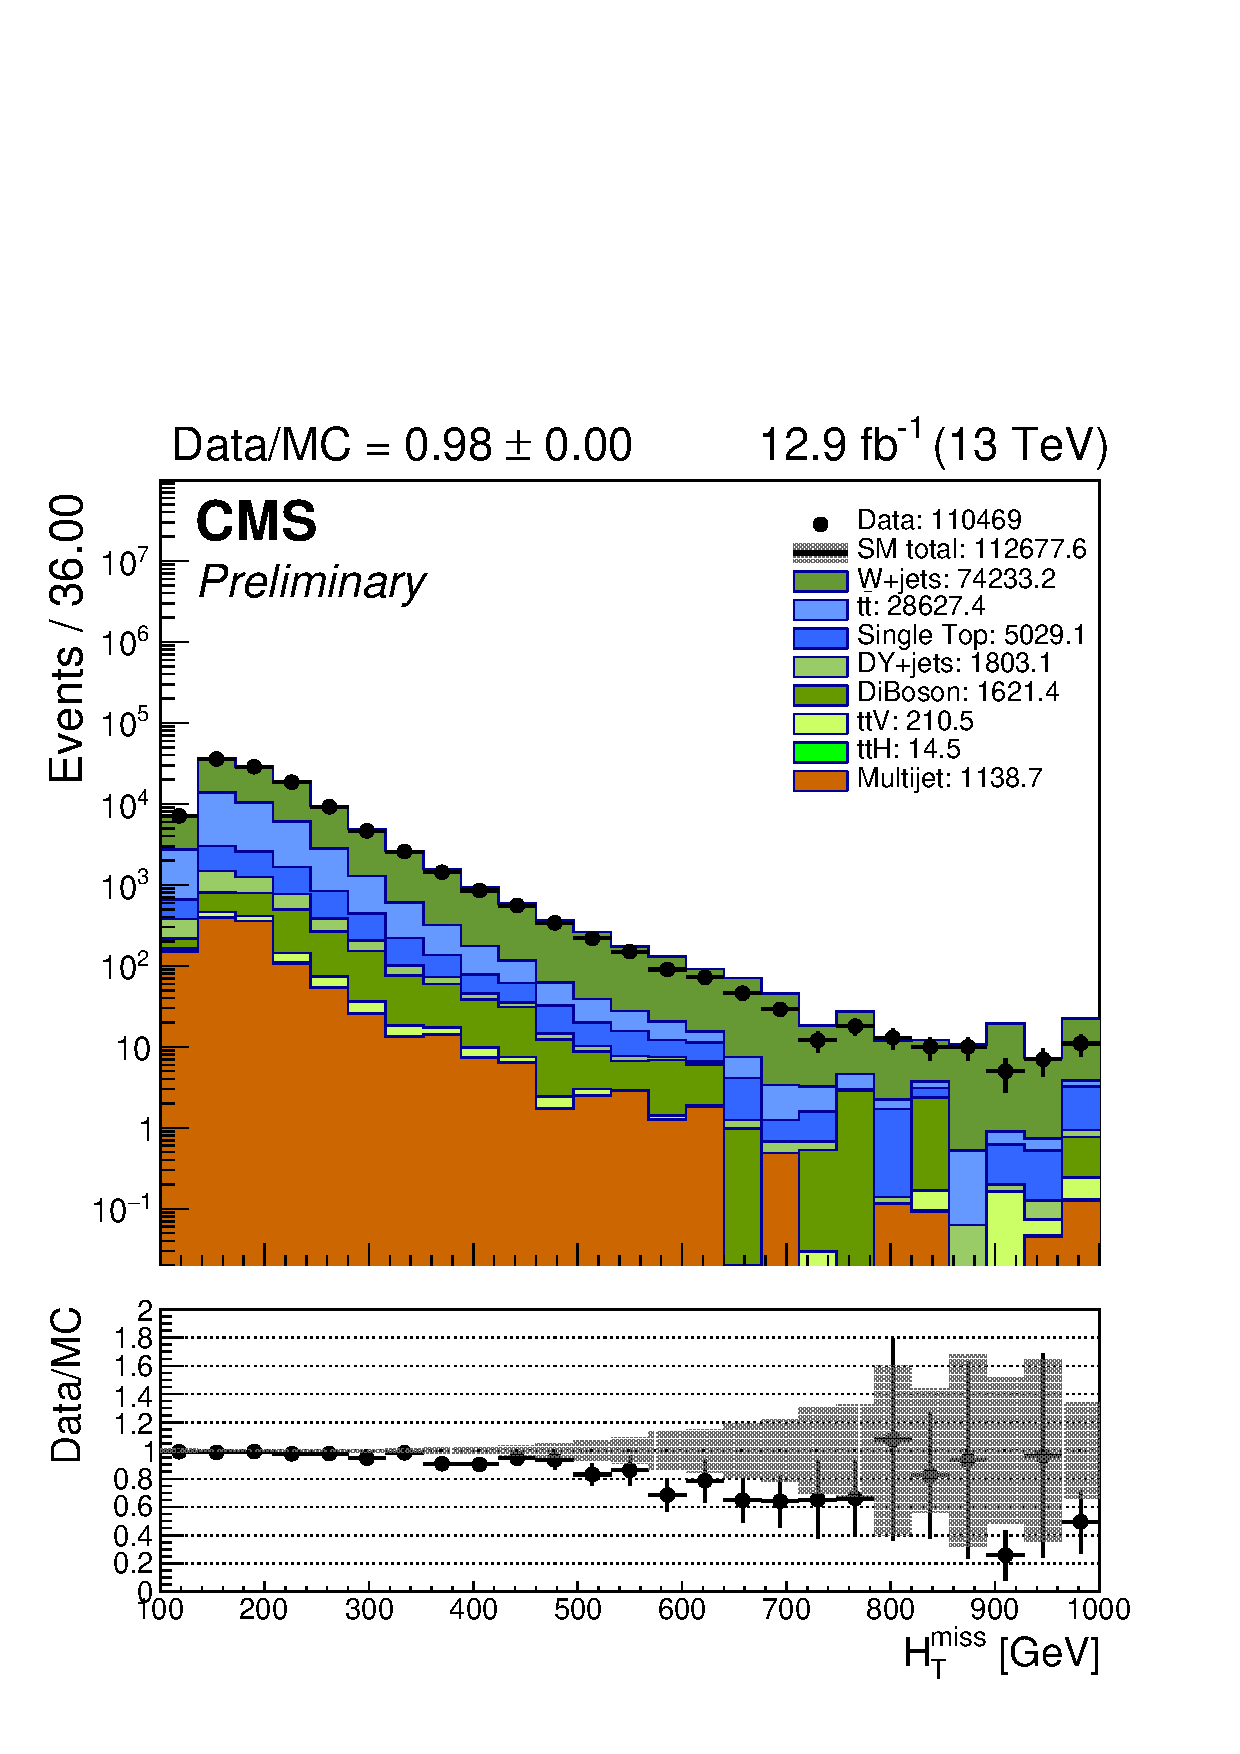
\includegraphics[width=0.5\textwidth]{figs/analysis/distributions/SingleMu/mht40_pt_asym.pdf}} ~~
        \subfloat {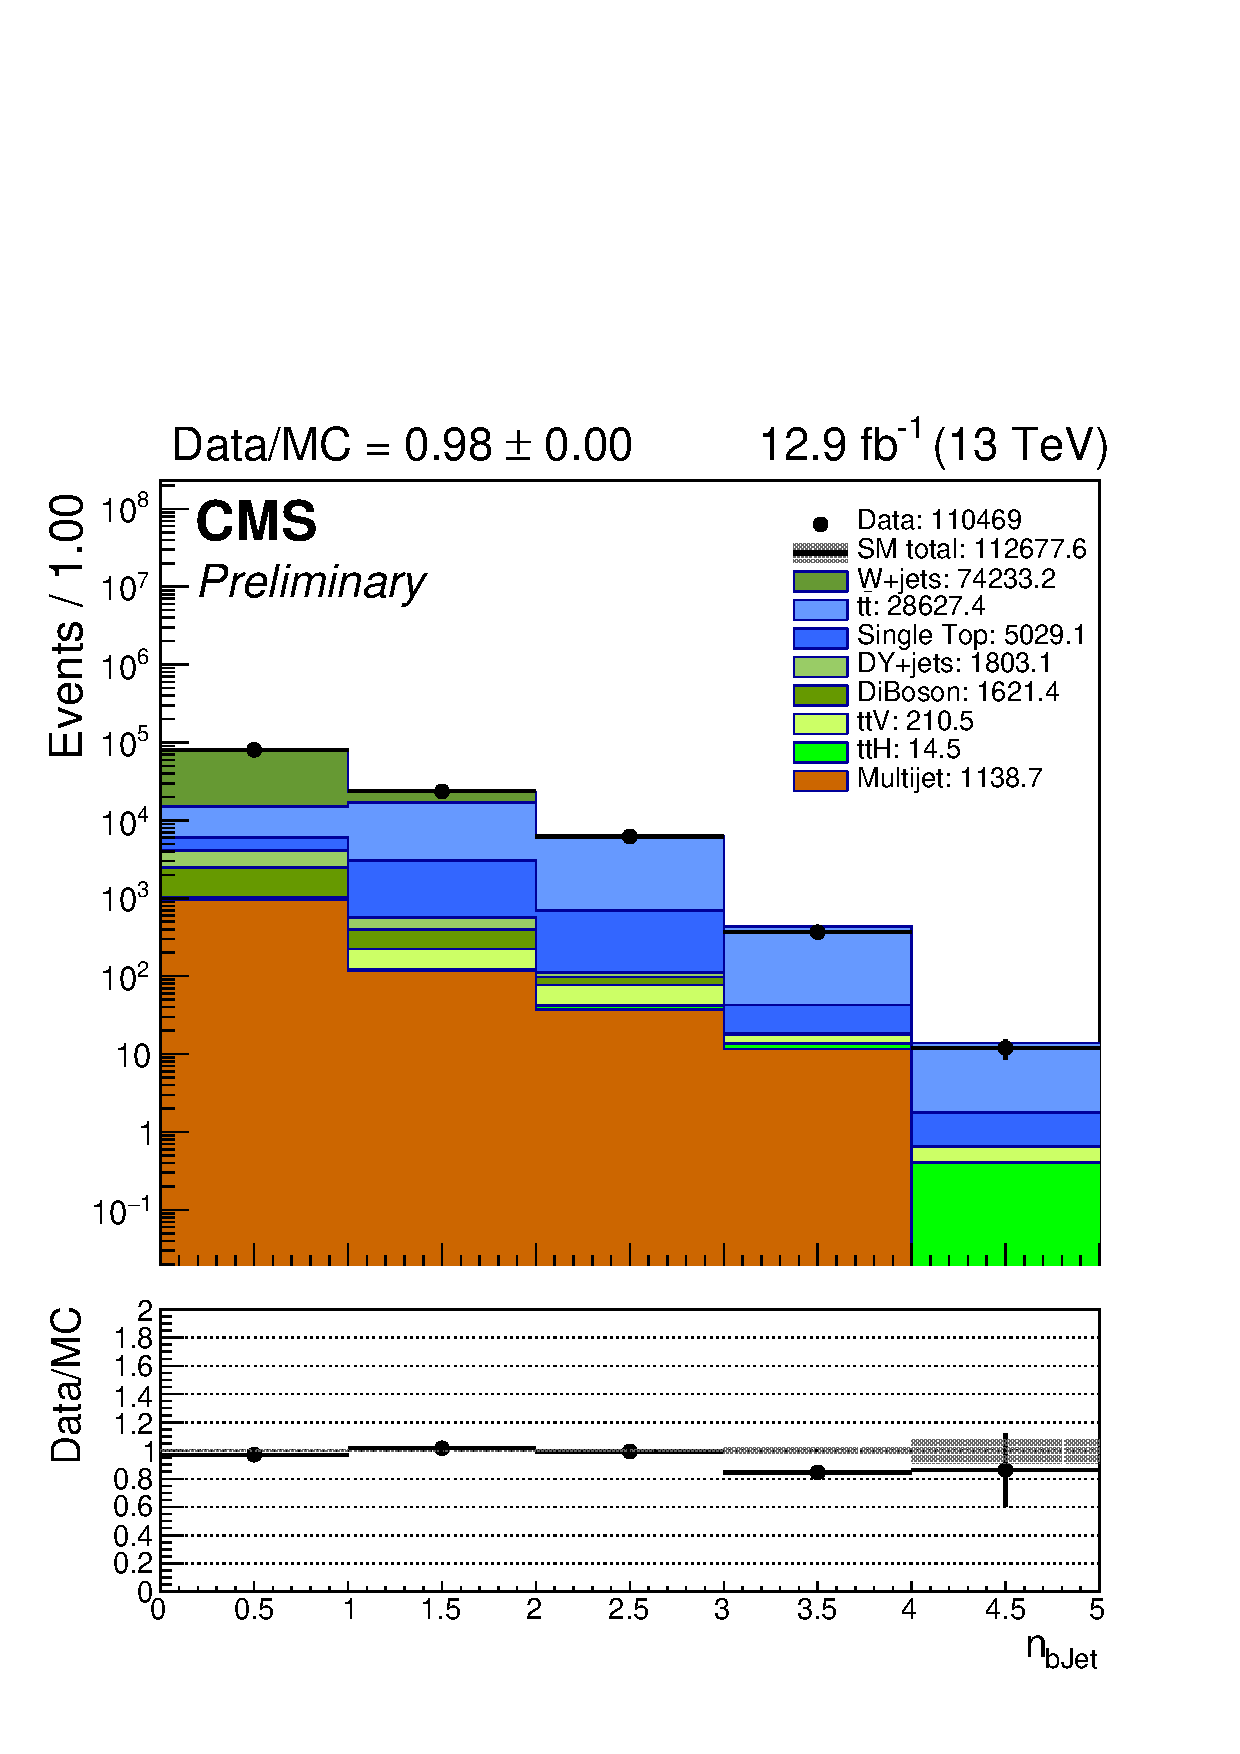
\includegraphics[width=0.5\textwidth]{figs/analysis/distributions/SingleMu/nBJet40_asym.pdf}} \\
        \caption{Key analysis variables for single muon control region (asymmetric \njet bins)}
        \label{fig:distribution_singlemu_asym}
    \end{center}
\end{figure}

\clearpage
\begin{figure}
    \begin{center}        
        \subfloat {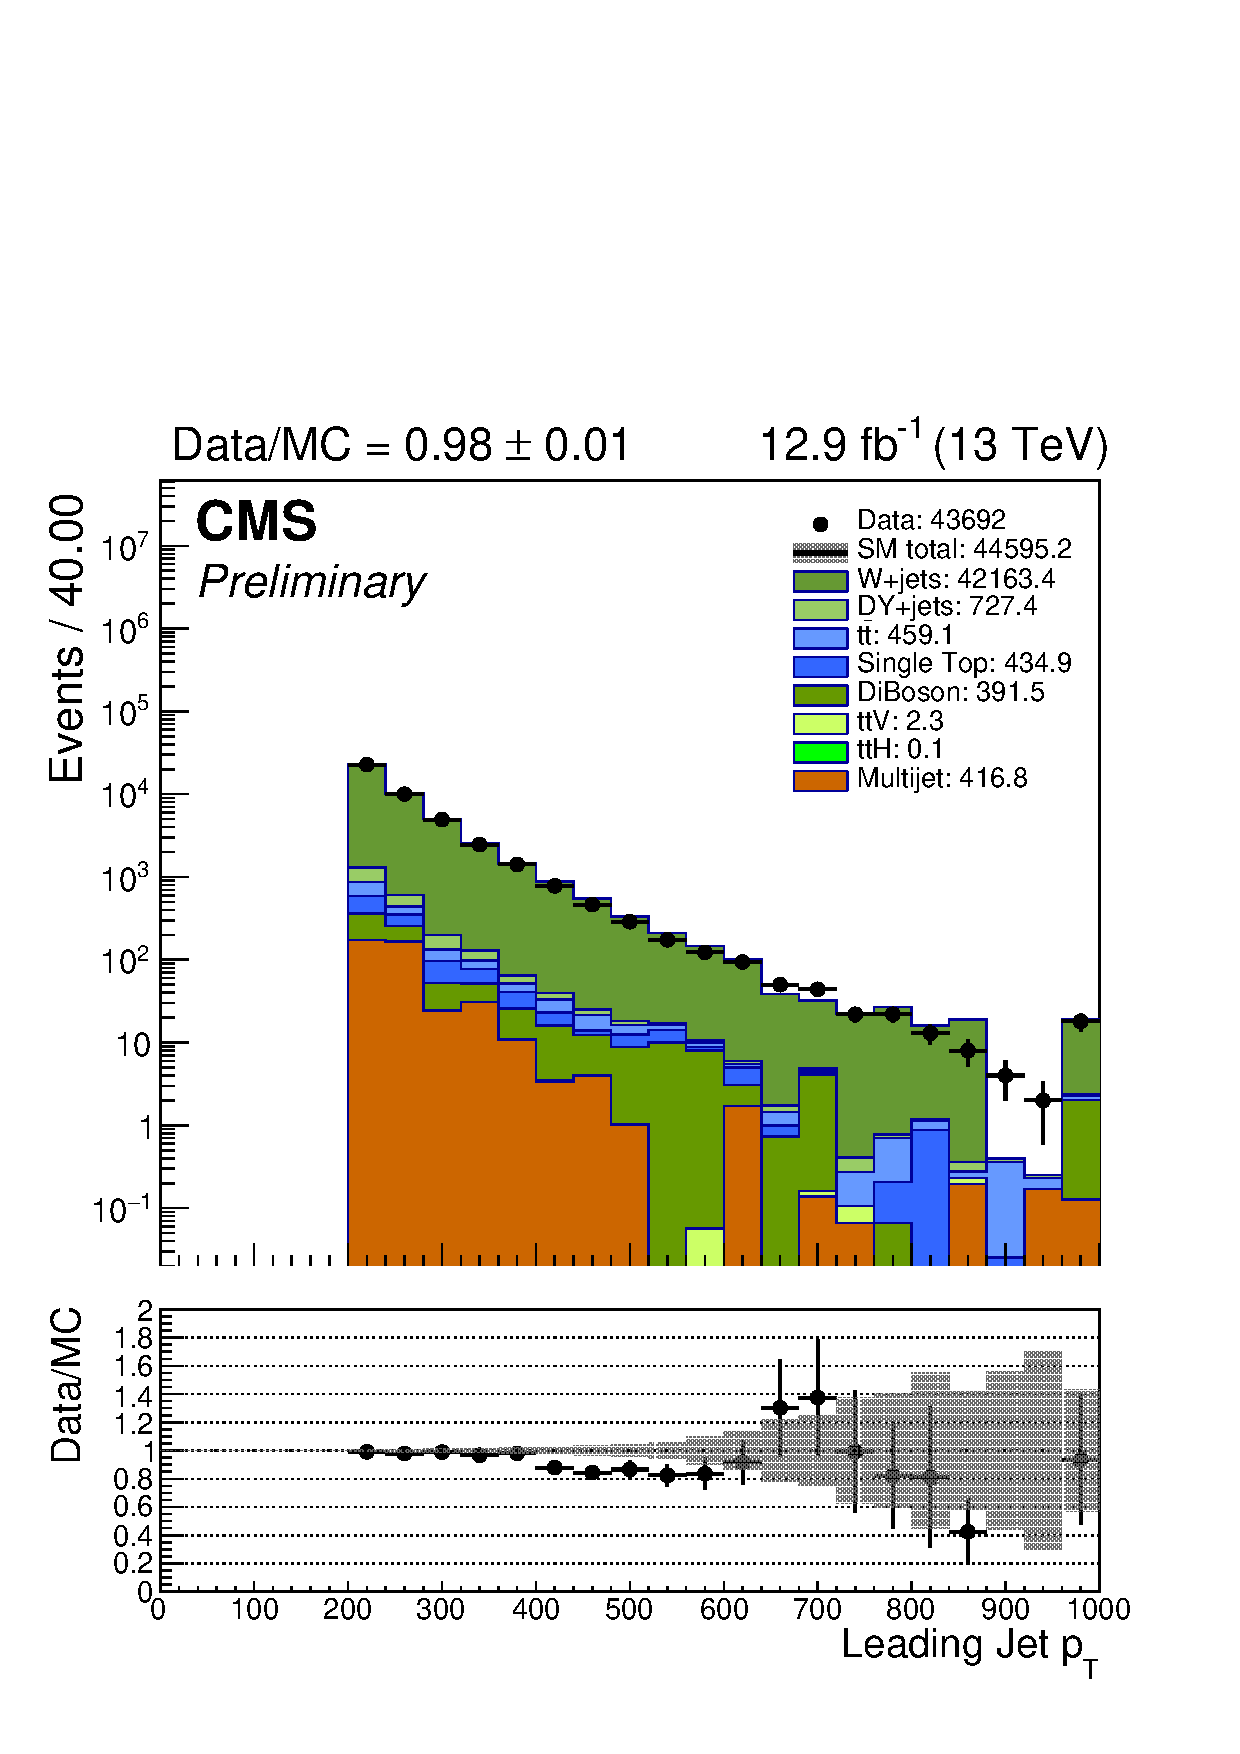
\includegraphics[width=0.5\textwidth]{figs/analysis/distributions/SingleMu/jet_pt[0]_eq1j.pdf}} ~~
        \subfloat {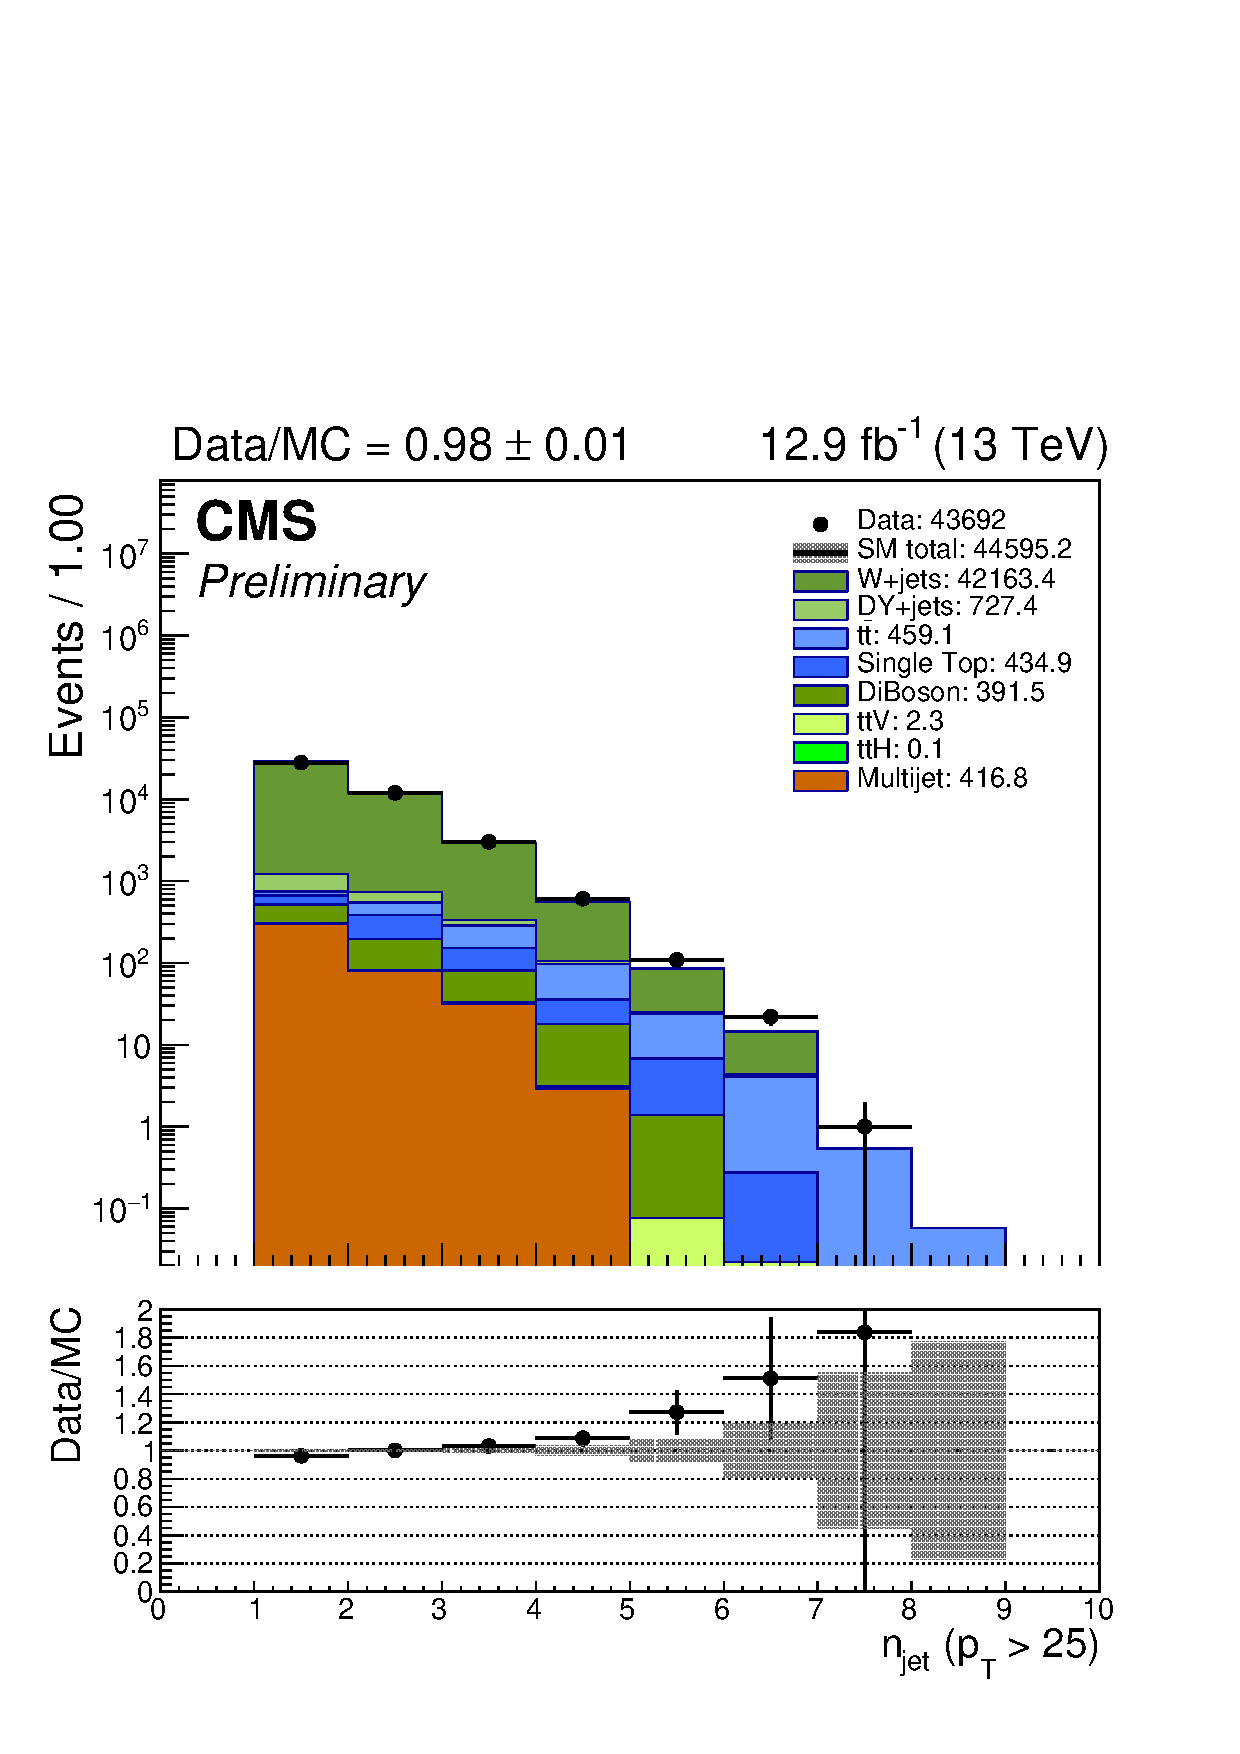
\includegraphics[width=0.5\textwidth]{figs/analysis/distributions/SingleMu/njetInc_eq1j.pdf}} \\
        \subfloat {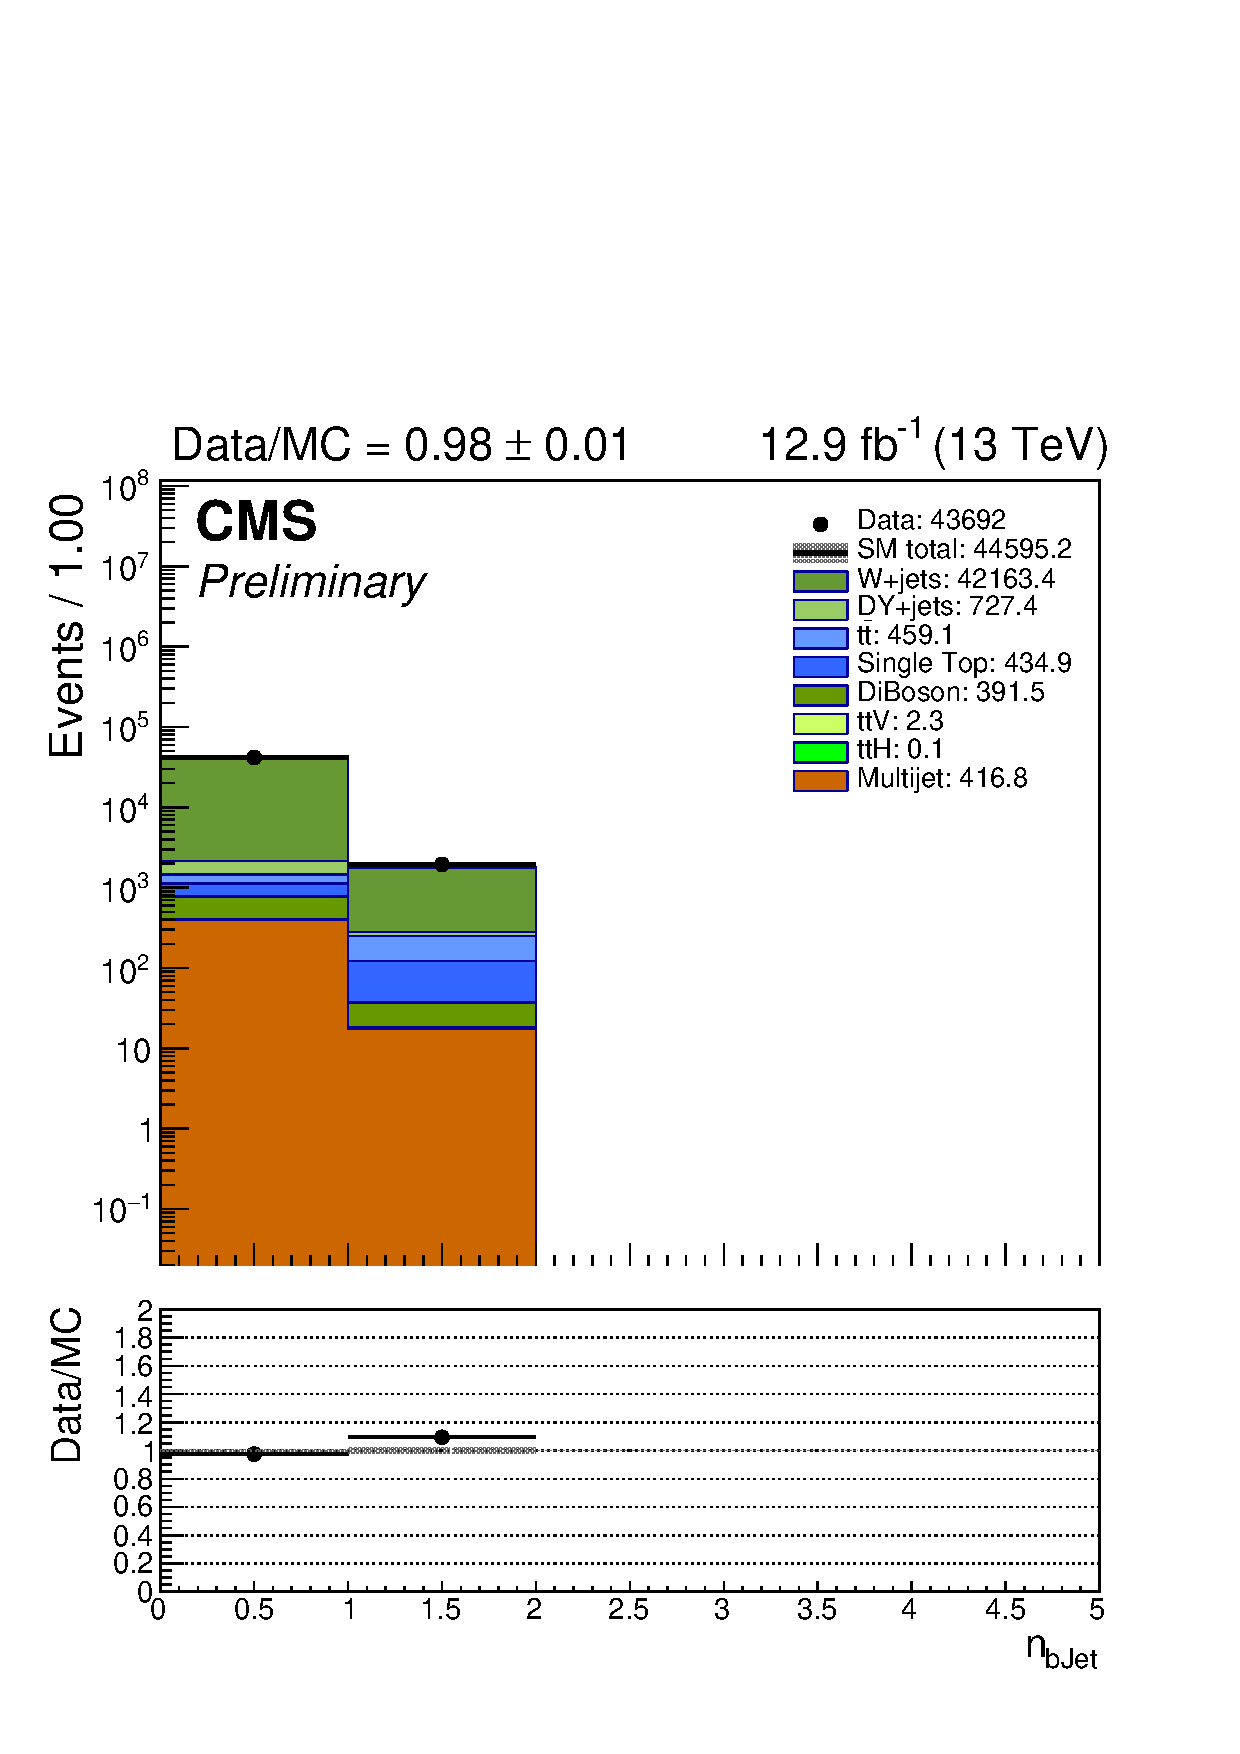
\includegraphics[width=0.5\textwidth]{figs/analysis/distributions/SingleMu/nBJet40_eq1j.pdf}} ~~
        \subfloat {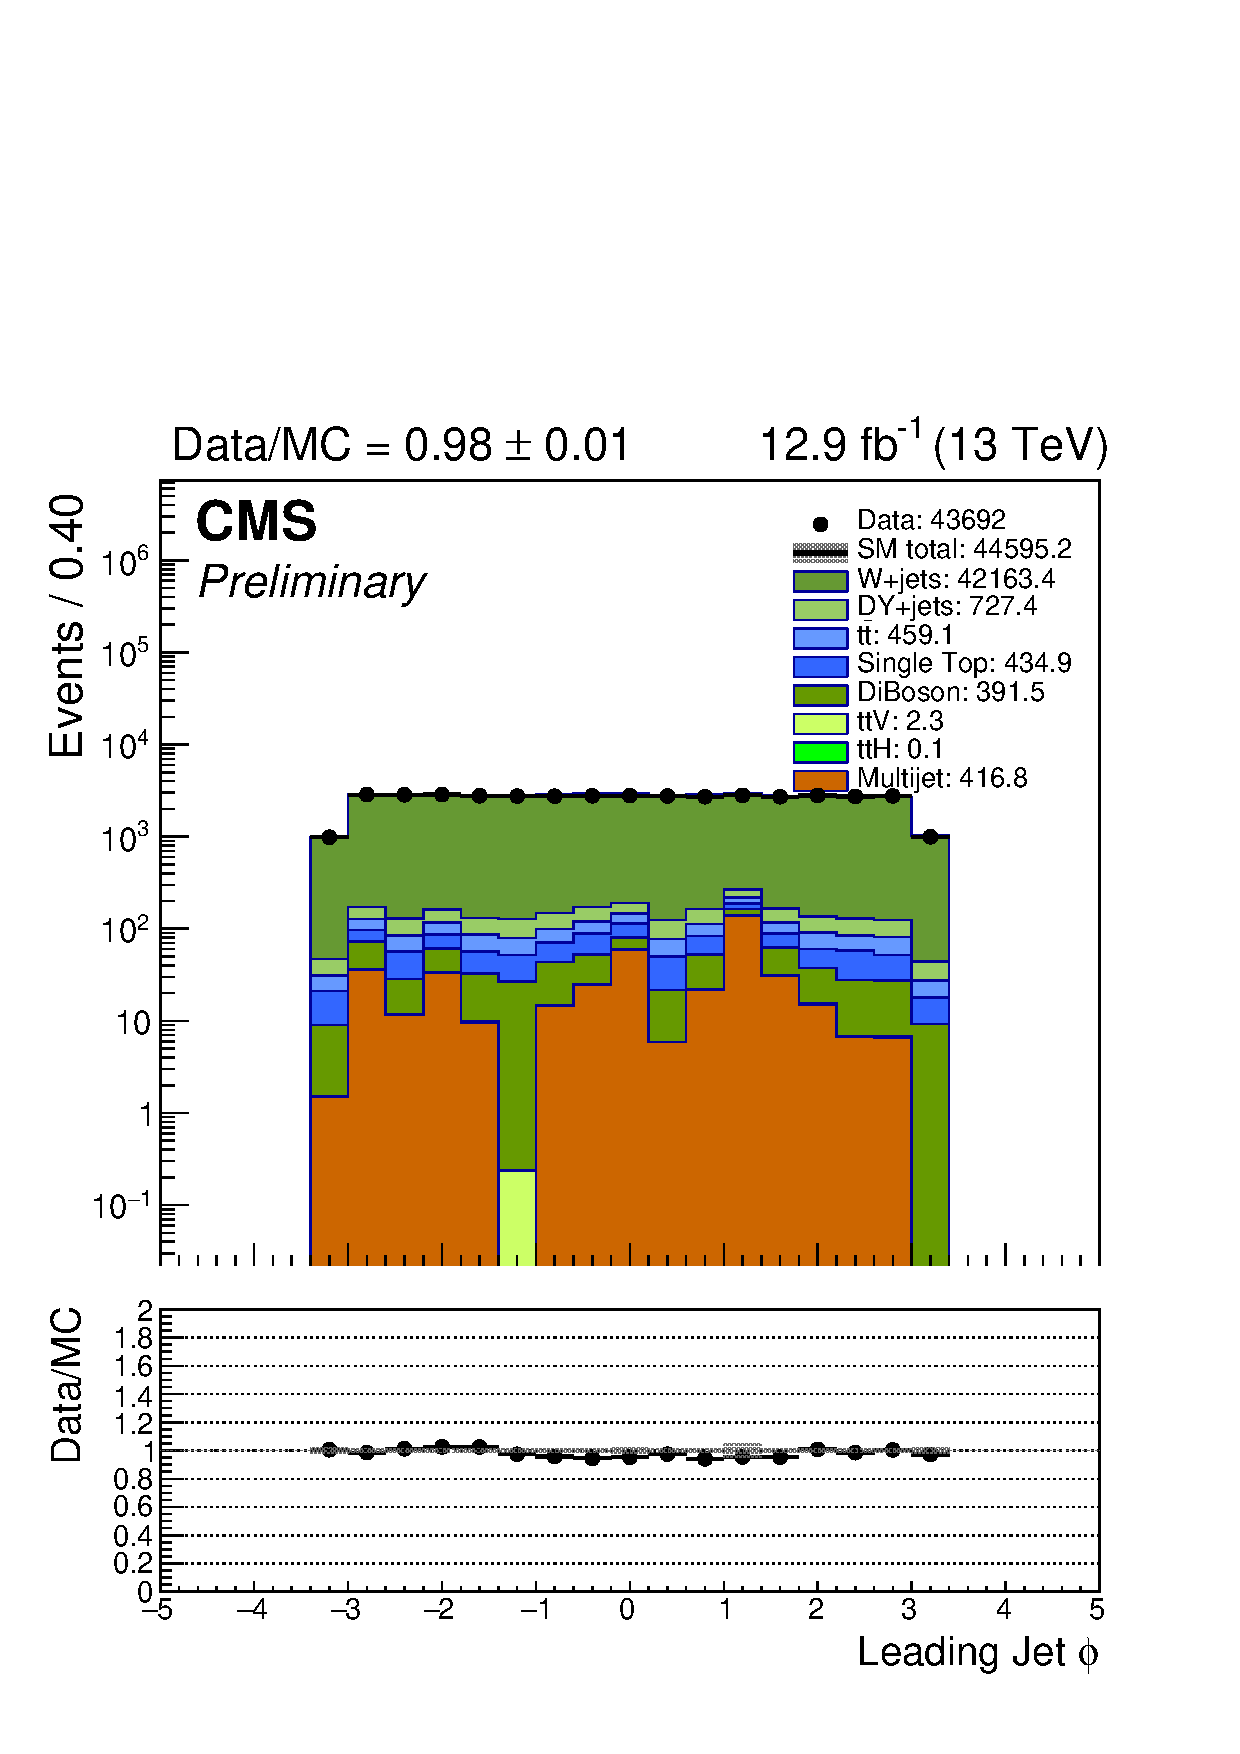
\includegraphics[width=0.5\textwidth]{figs/analysis/distributions/SingleMu/jet_phi[0]_eq1j.pdf}} \\
        \caption{Key analysis variables for single muon control region (monojet bins)}
        \label{fig:distribution_singlemu_mono}
    \end{center}
\end{figure}

% \clearpage
% \subsection{Yields and distributions for the di-muon + jets control sample}

\begin{figure}
    \begin{center}
        \subfloat {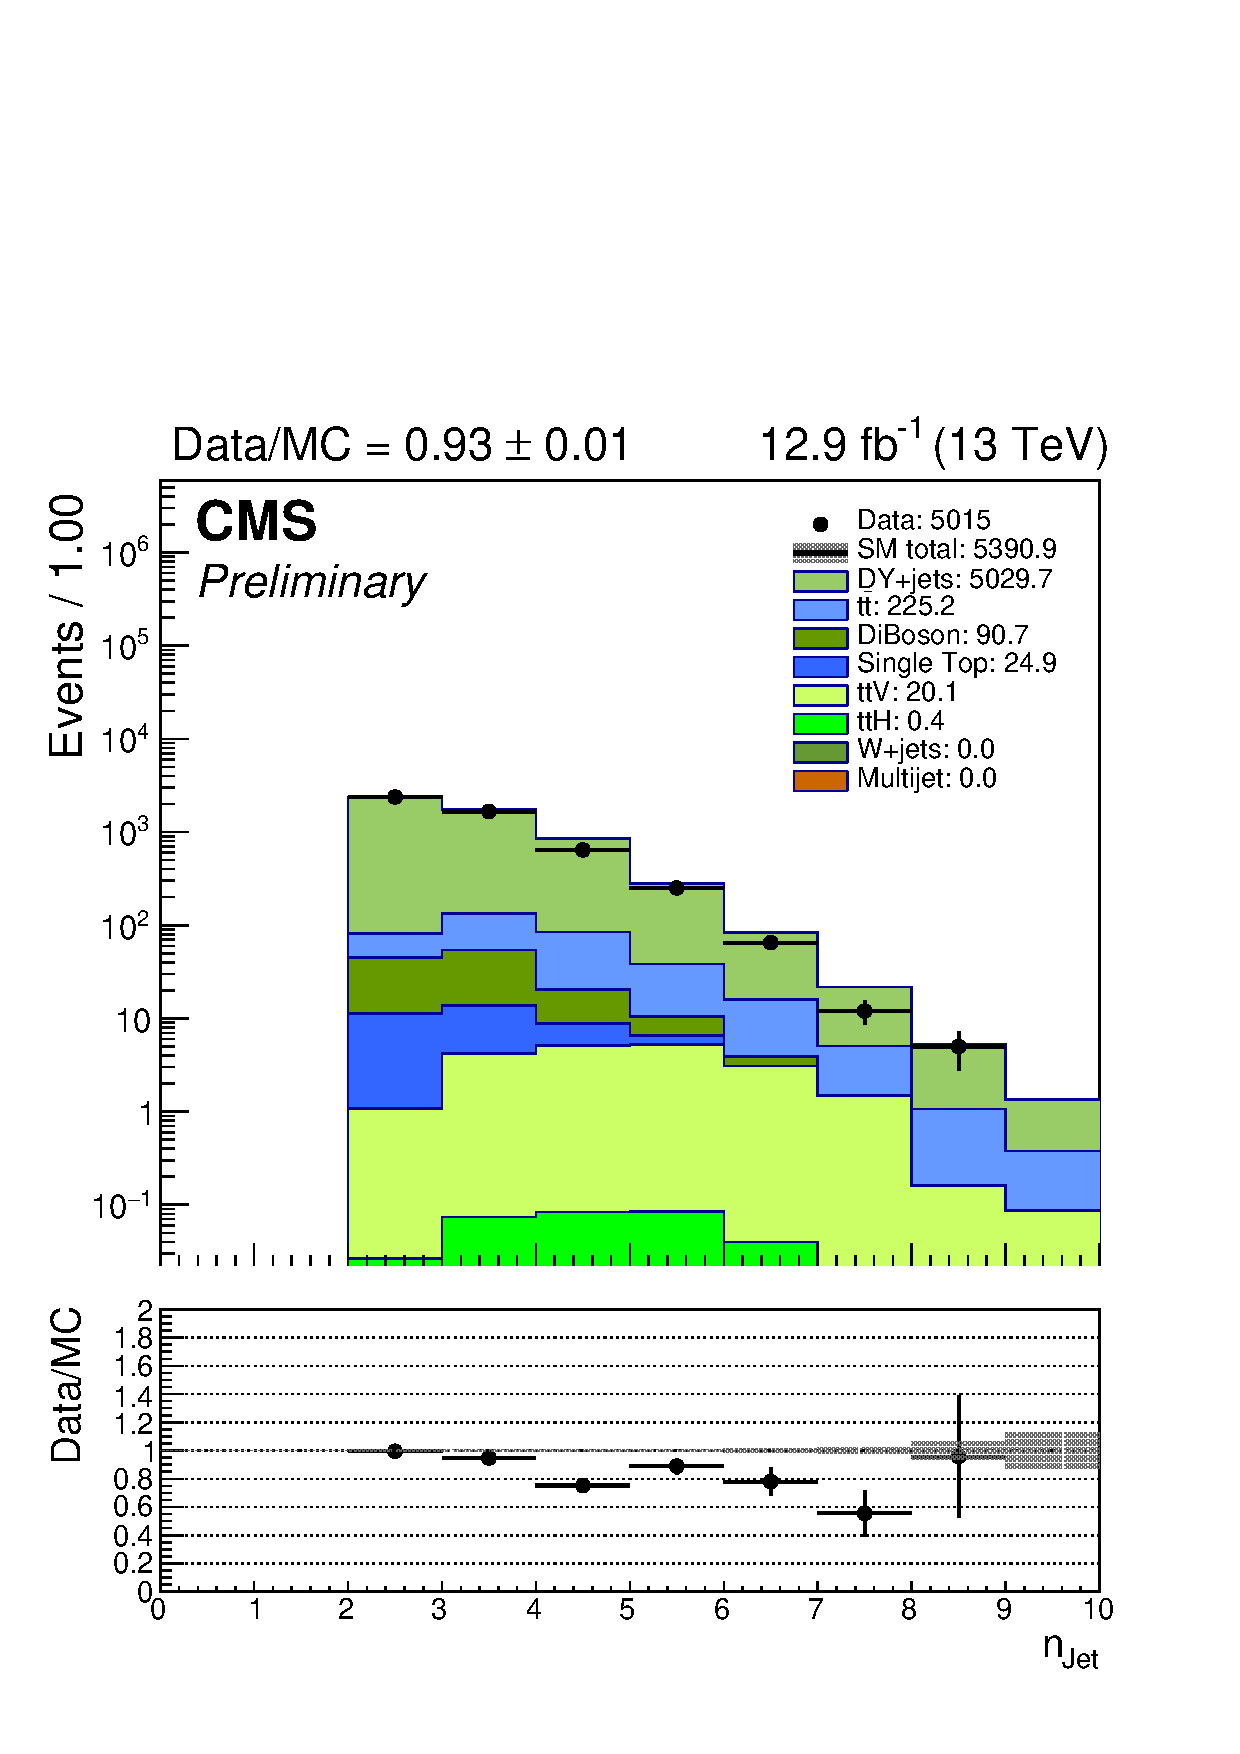
\includegraphics[width=0.5\textwidth]{figs/analysis/distributions/DoubleMu/nJet40_sym.pdf}} ~~
        \subfloat {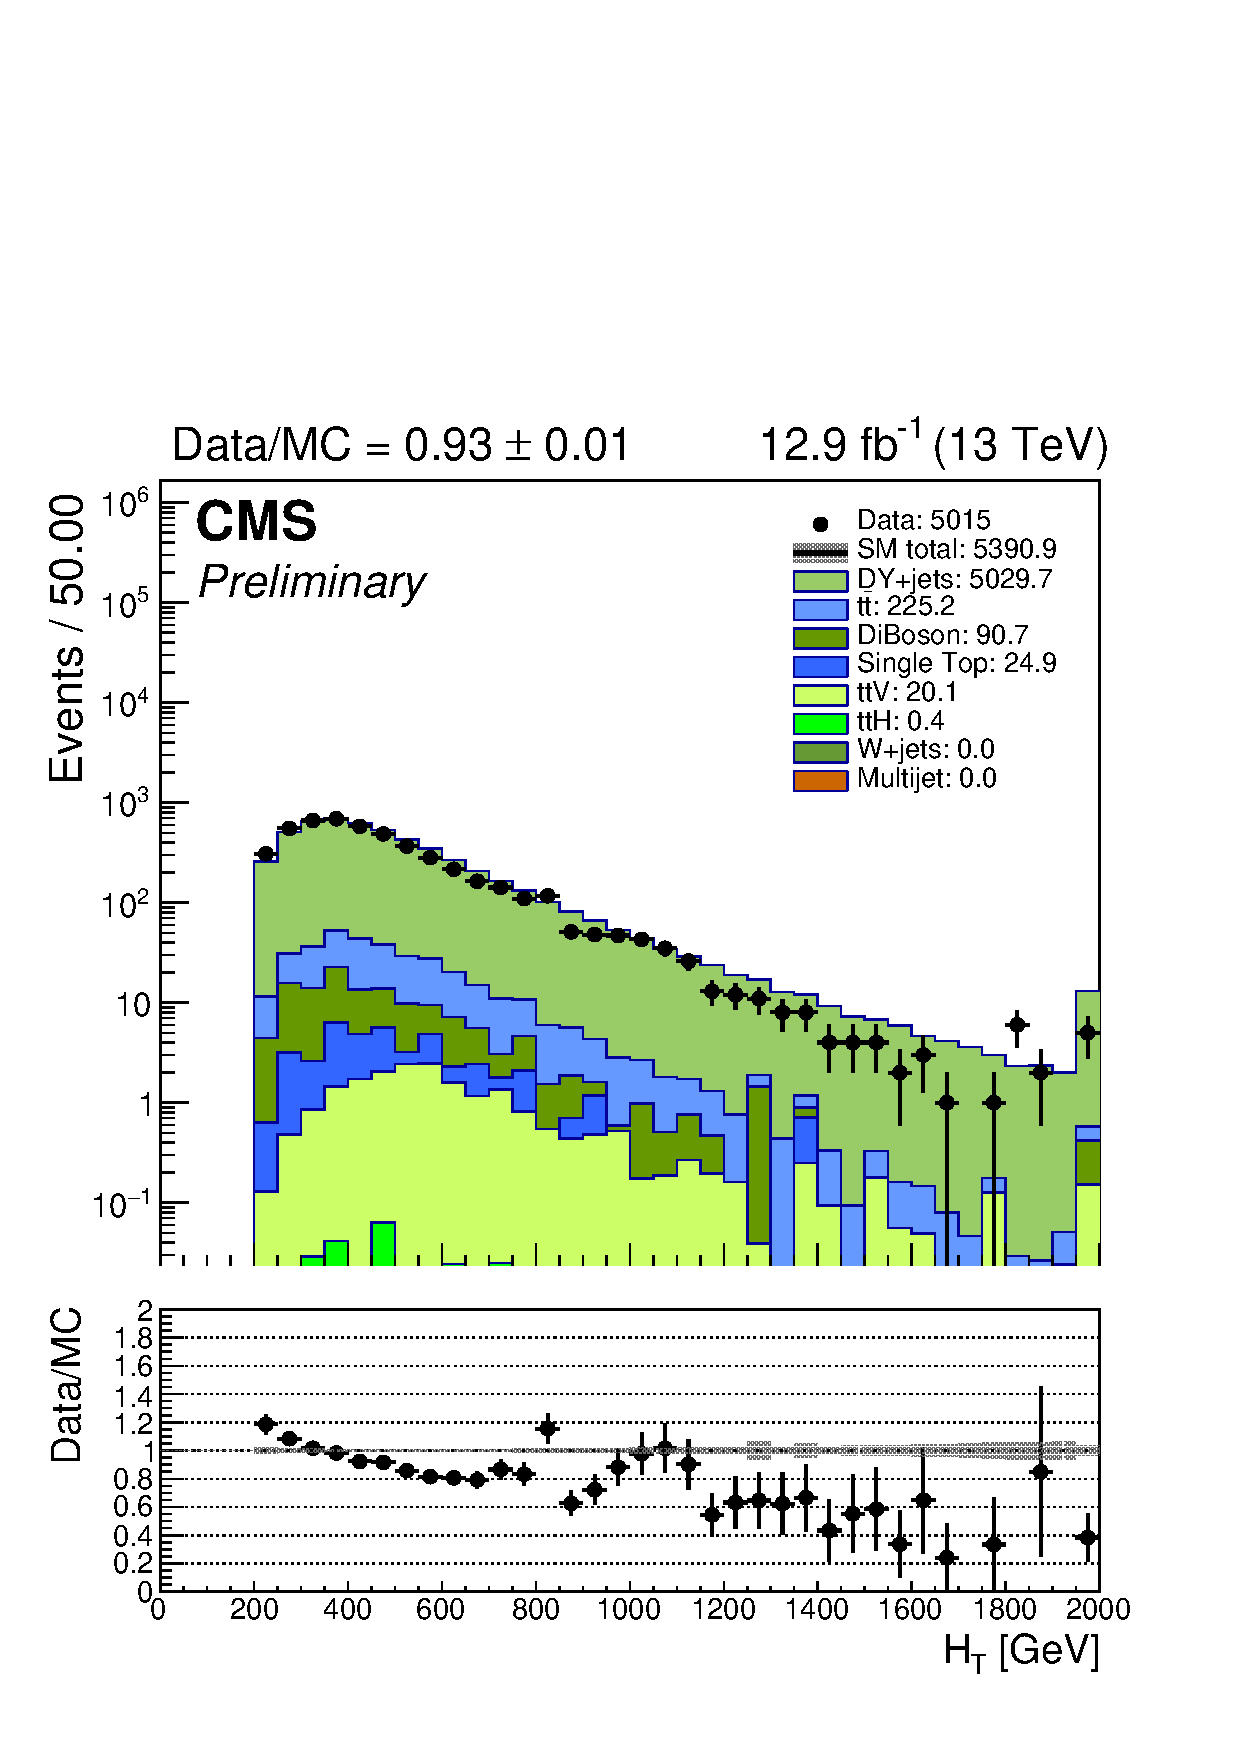
\includegraphics[width=0.5\textwidth]{figs/analysis/distributions/DoubleMu/ht40_sym.pdf}} \\
        \subfloat {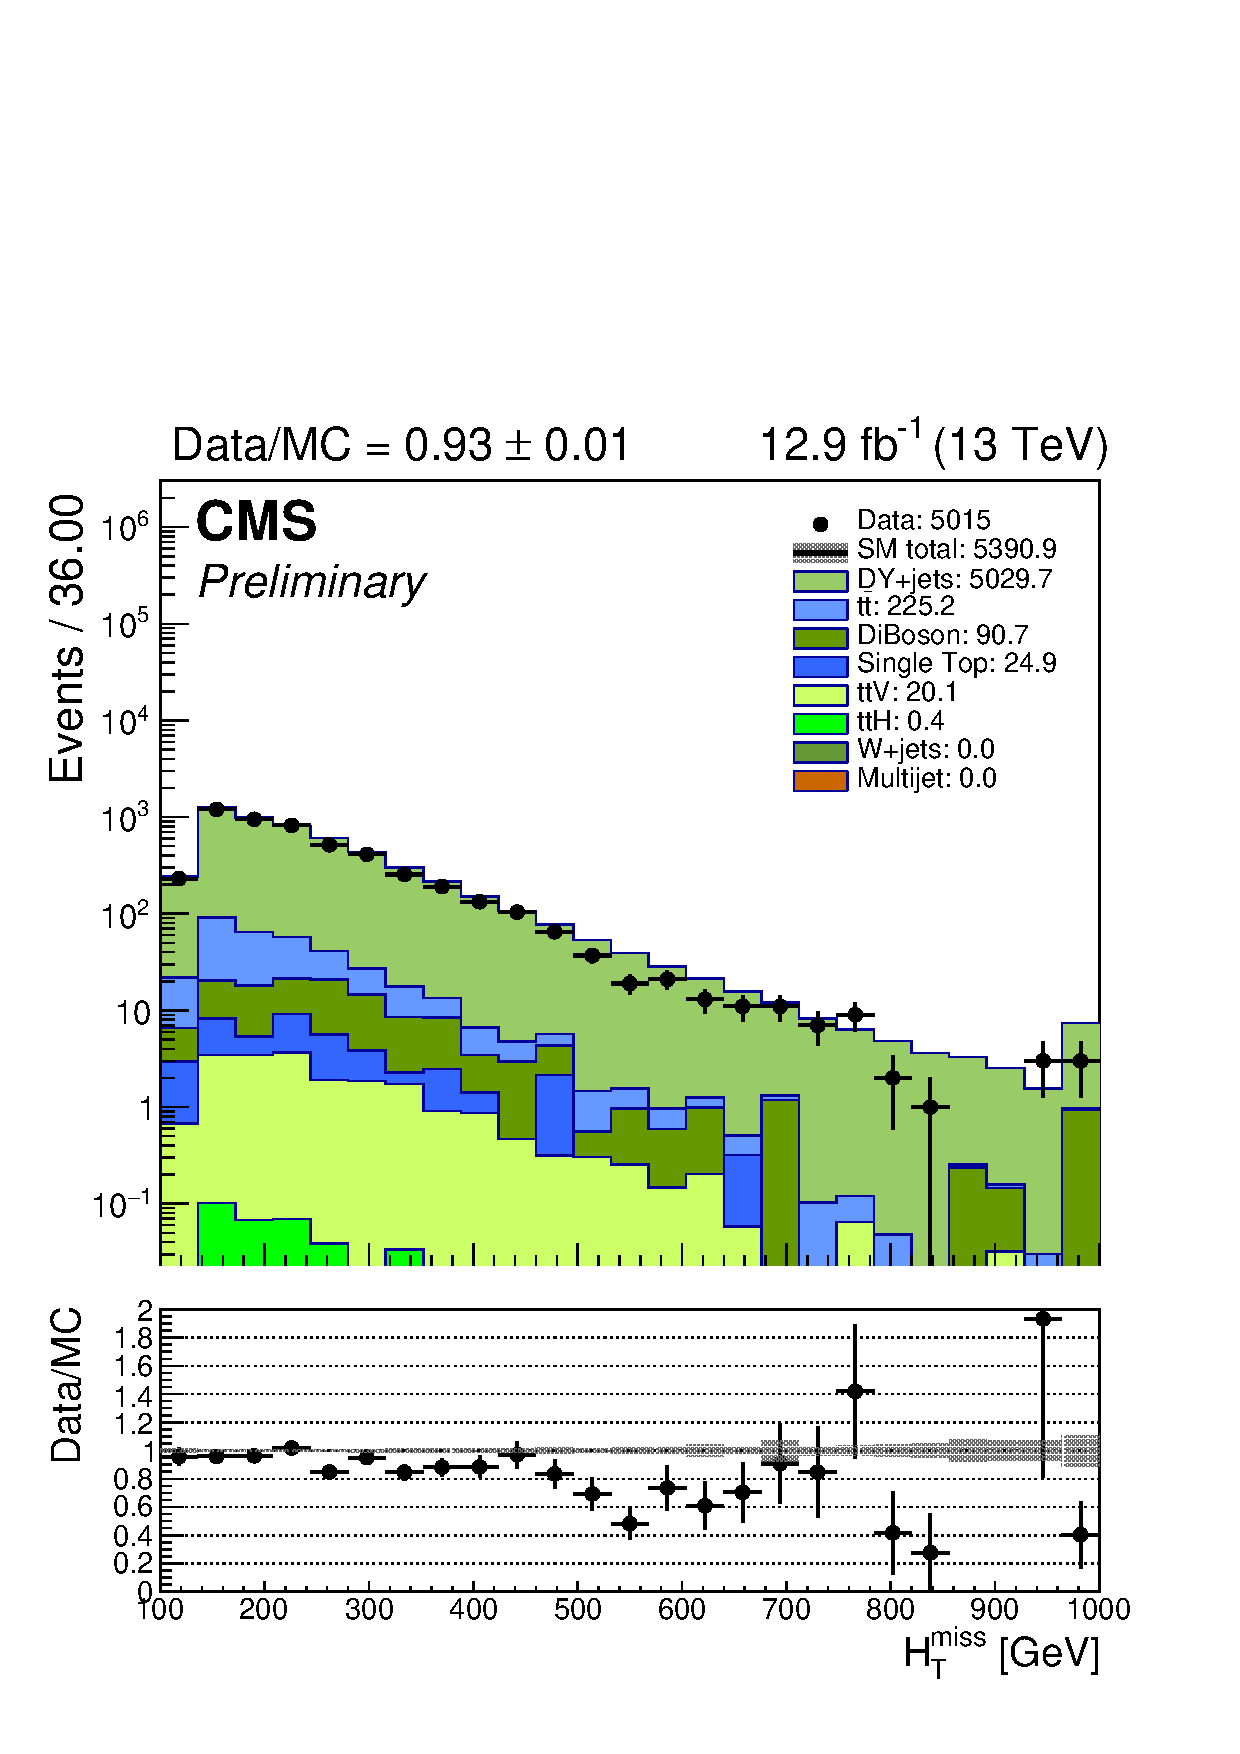
\includegraphics[width=0.5\textwidth]{figs/analysis/distributions/DoubleMu/mht40_pt_sym.pdf}} ~~
        \subfloat {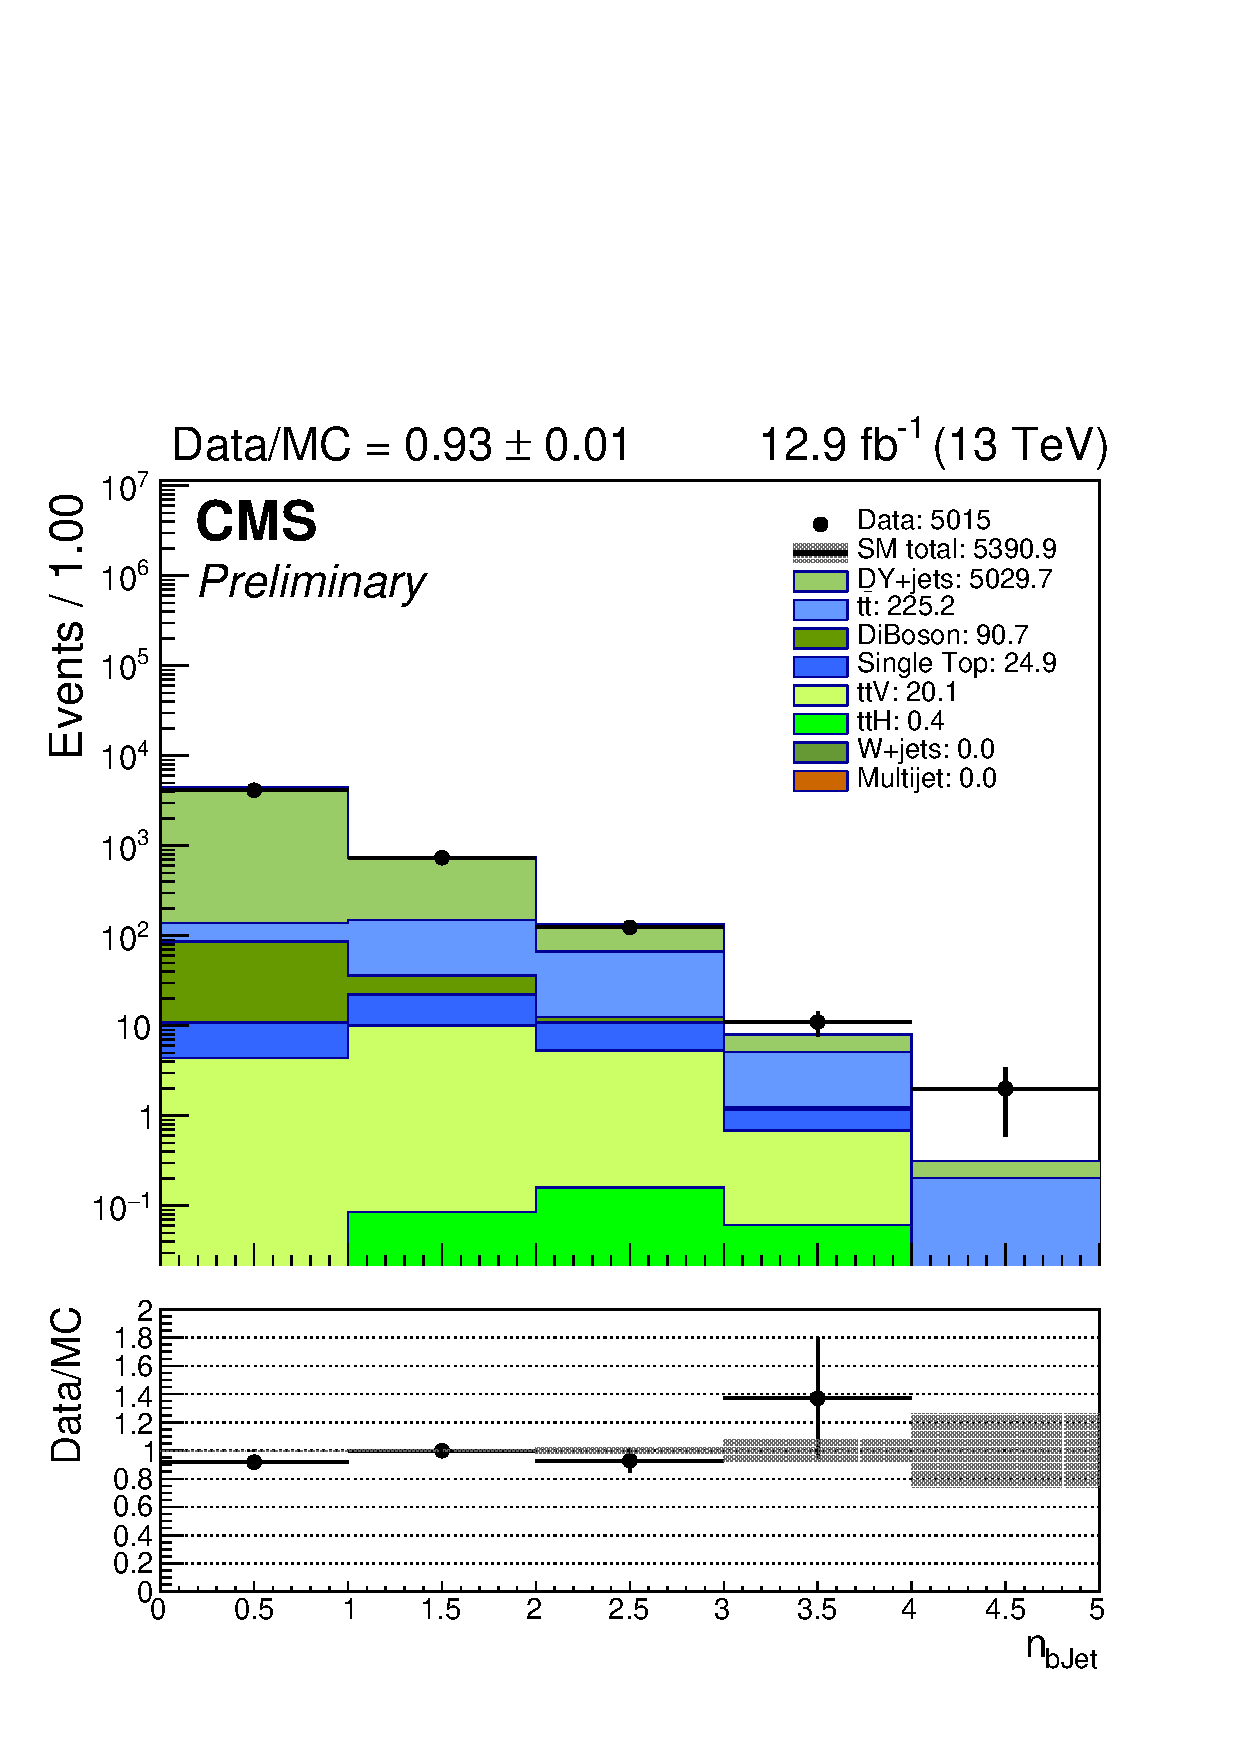
\includegraphics[width=0.5\textwidth]{figs/analysis/distributions/DoubleMu/nBJet40_sym.pdf}} \\
        \caption{Key analysis variables for double muon control region (symmetric \njet bins)}
        \label{fig:distribution_doublemu_sym}
    \end{center}
\end{figure}

\clearpage
\begin{figure}
    \begin{center}
        \subfloat {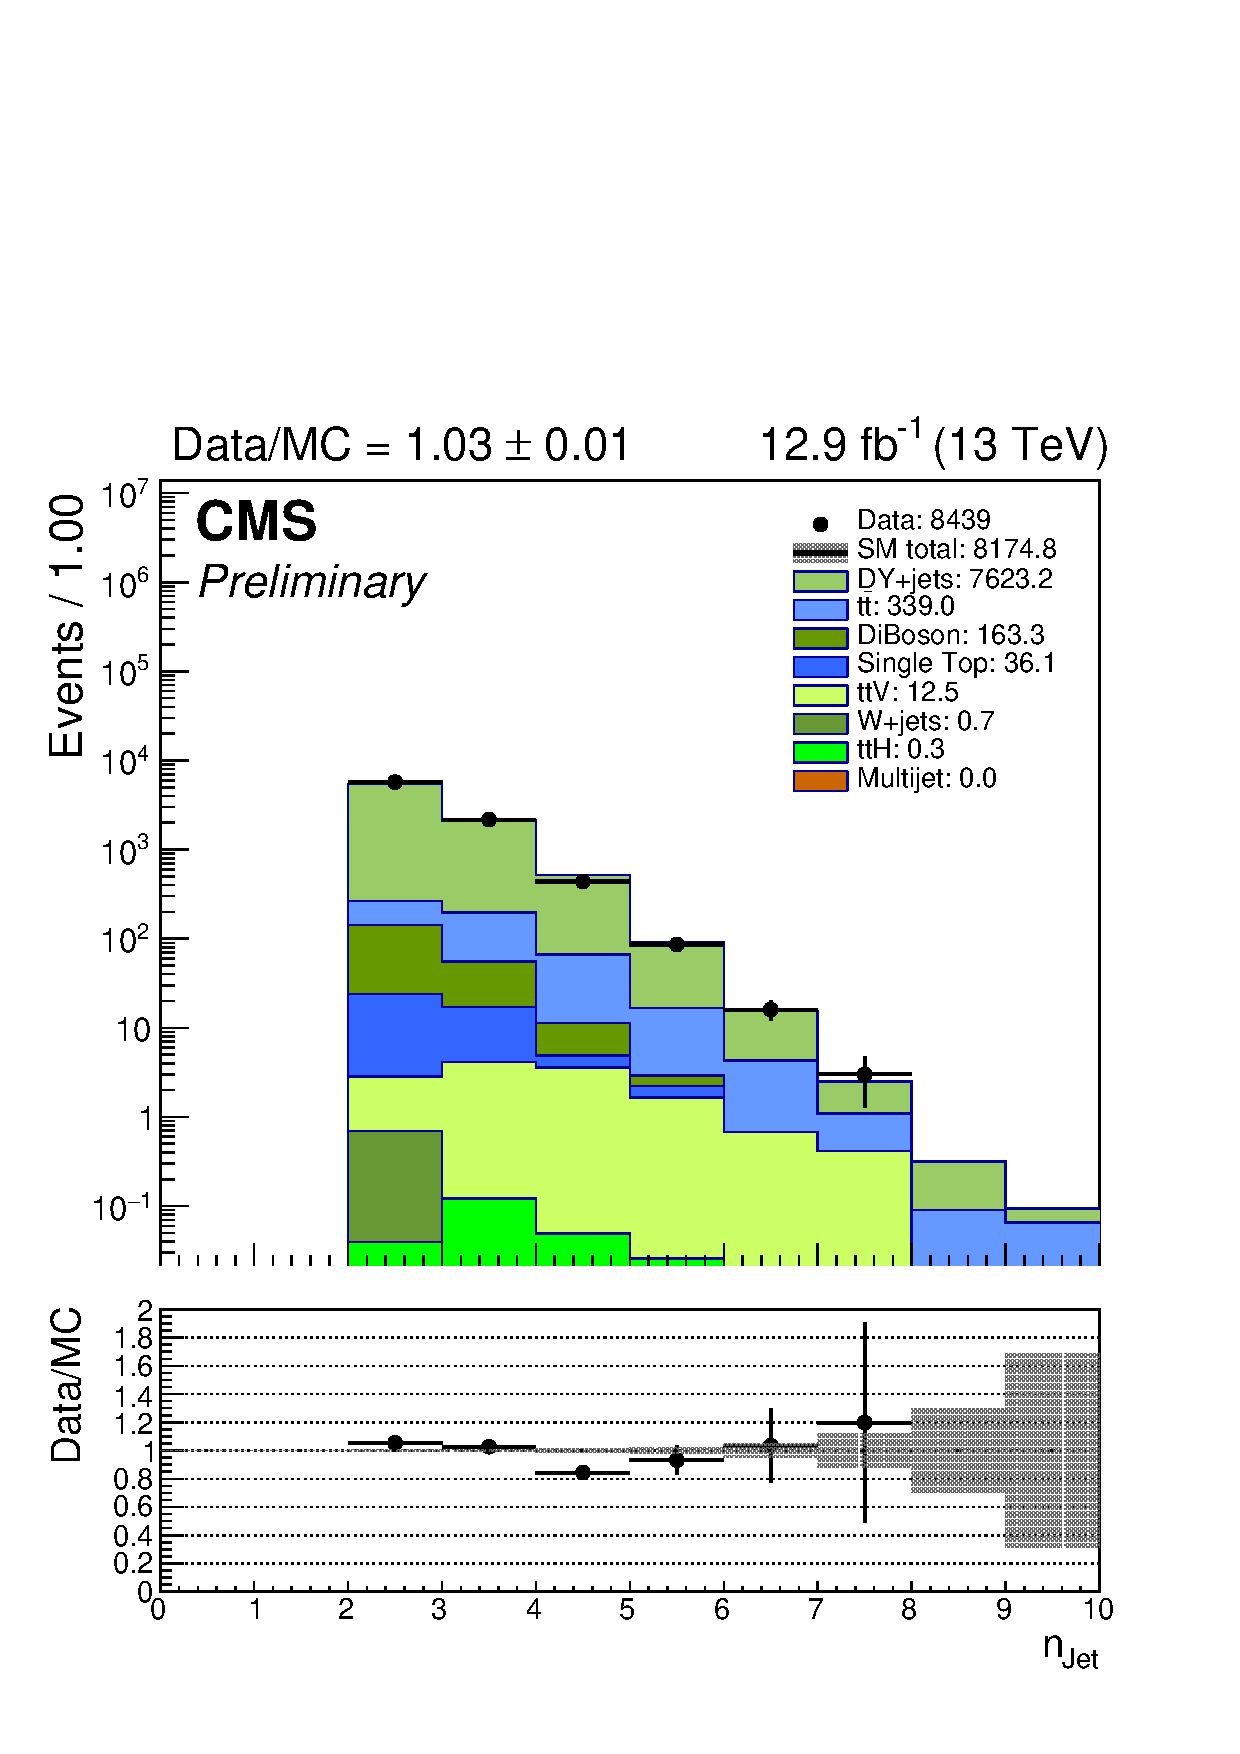
\includegraphics[width=0.5\textwidth]{figs/analysis/distributions/DoubleMu/nJet40_asym.pdf}} ~~
        \subfloat {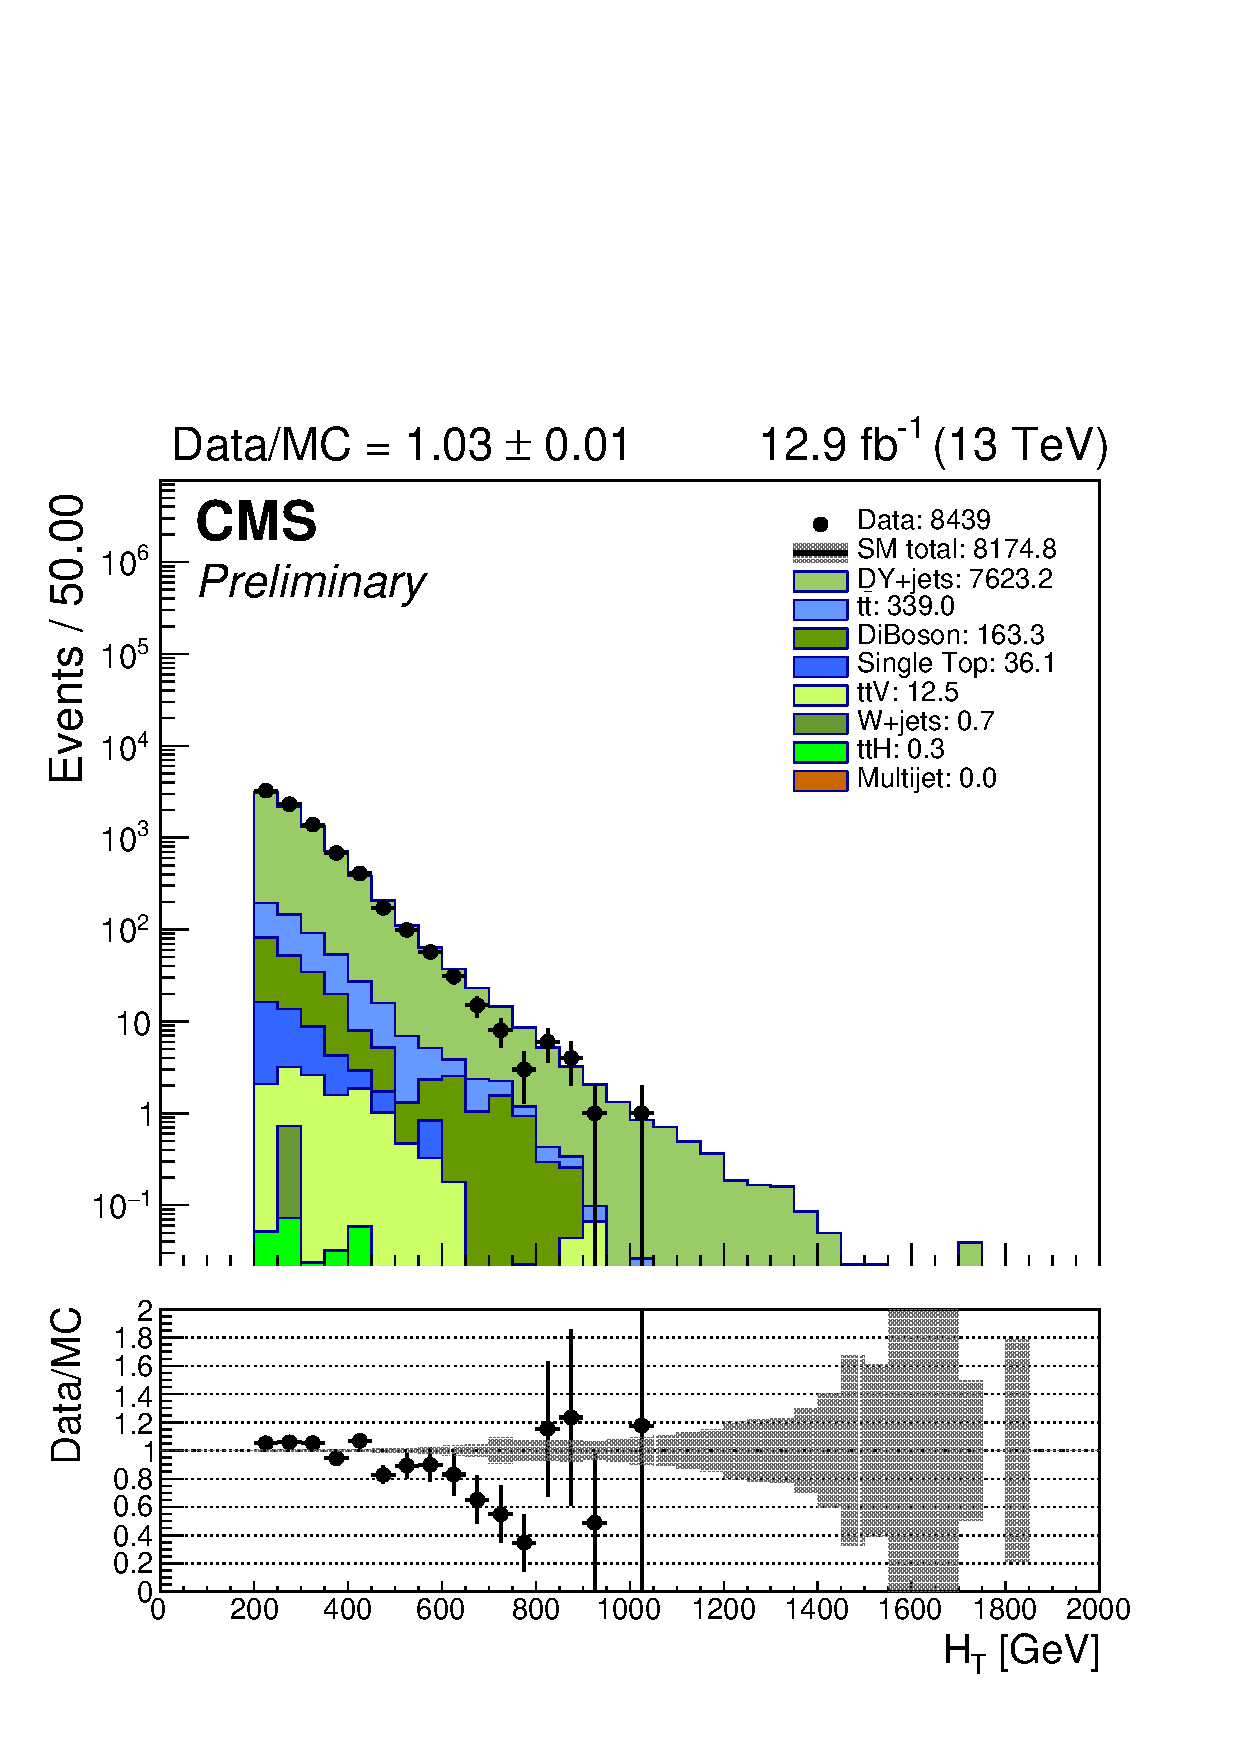
\includegraphics[width=0.5\textwidth]{figs/analysis/distributions/DoubleMu/ht40_asym.pdf}} \\
        \subfloat {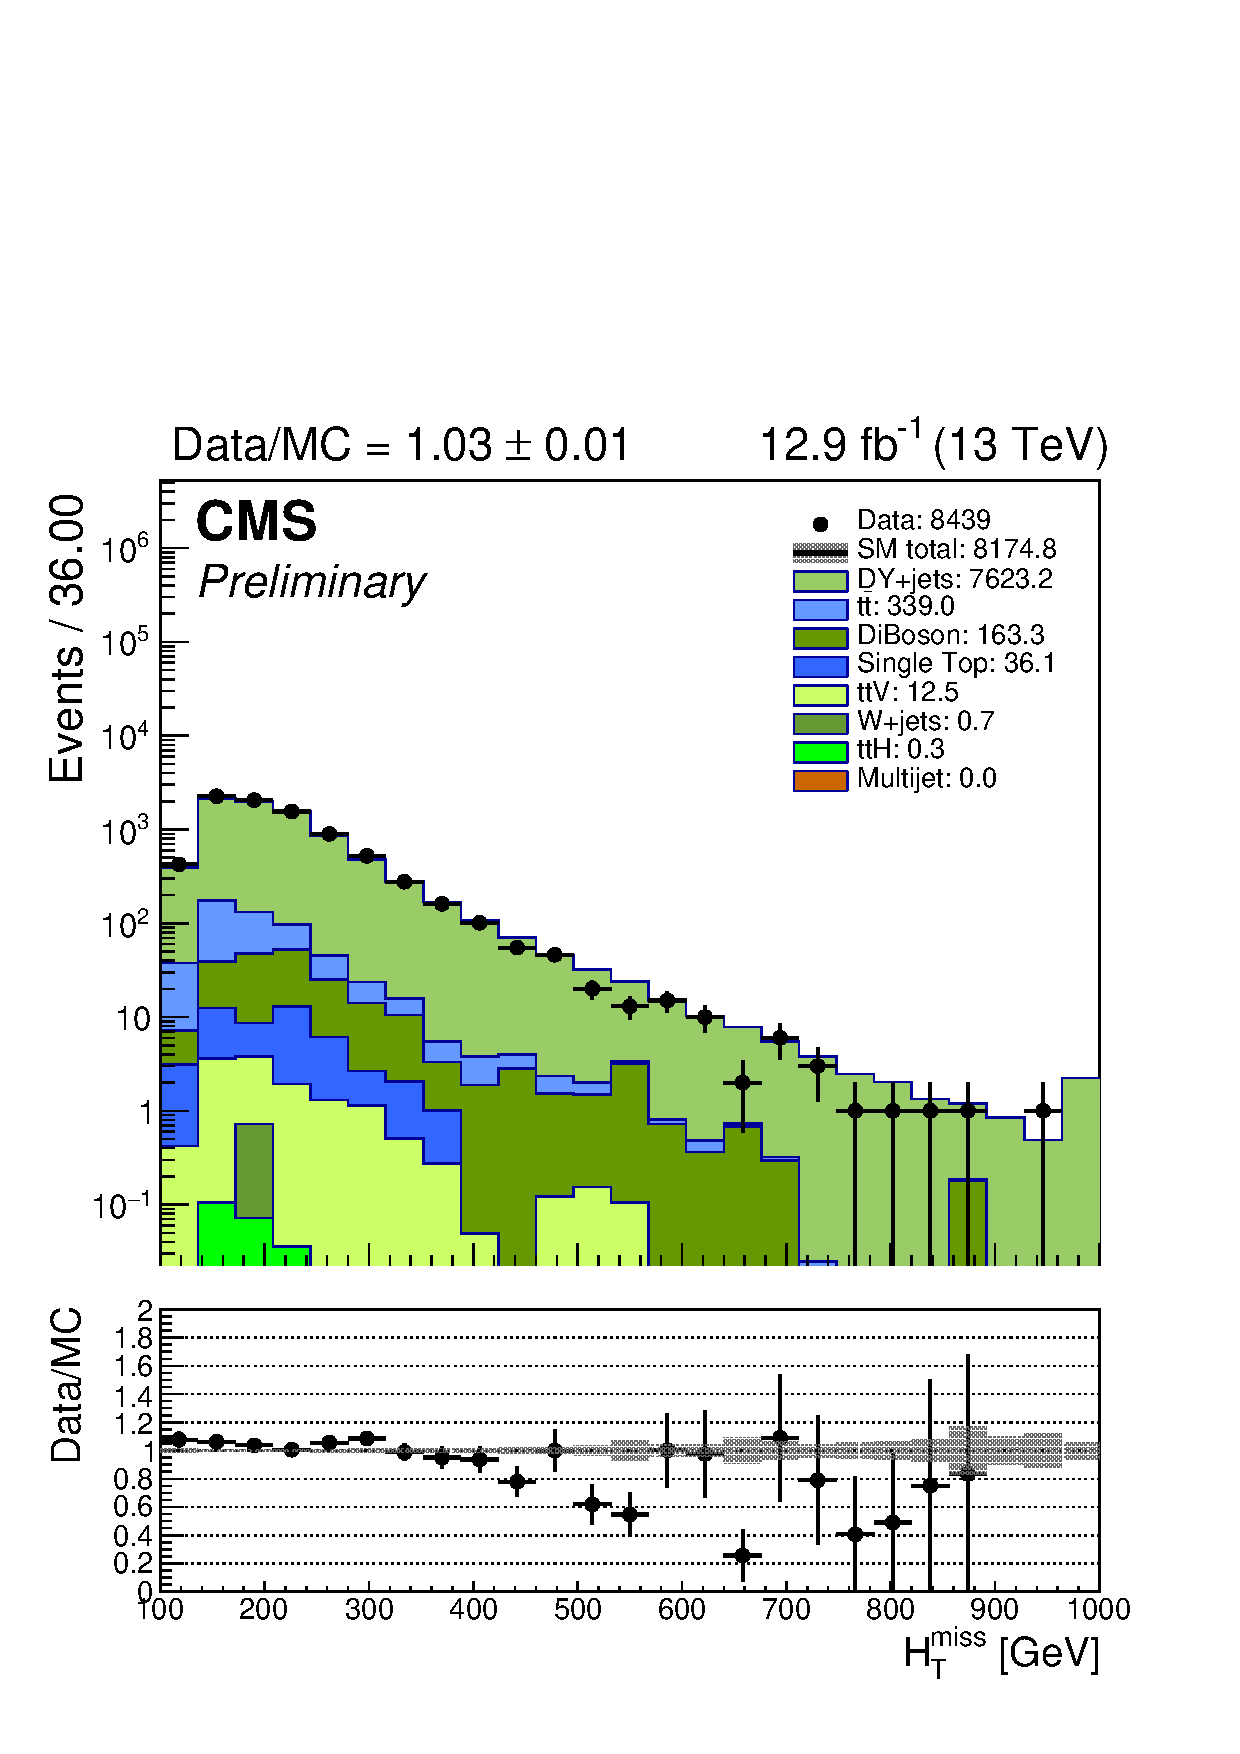
\includegraphics[width=0.5\textwidth]{figs/analysis/distributions/DoubleMu/mht40_pt_asym.pdf}} ~~
        \subfloat {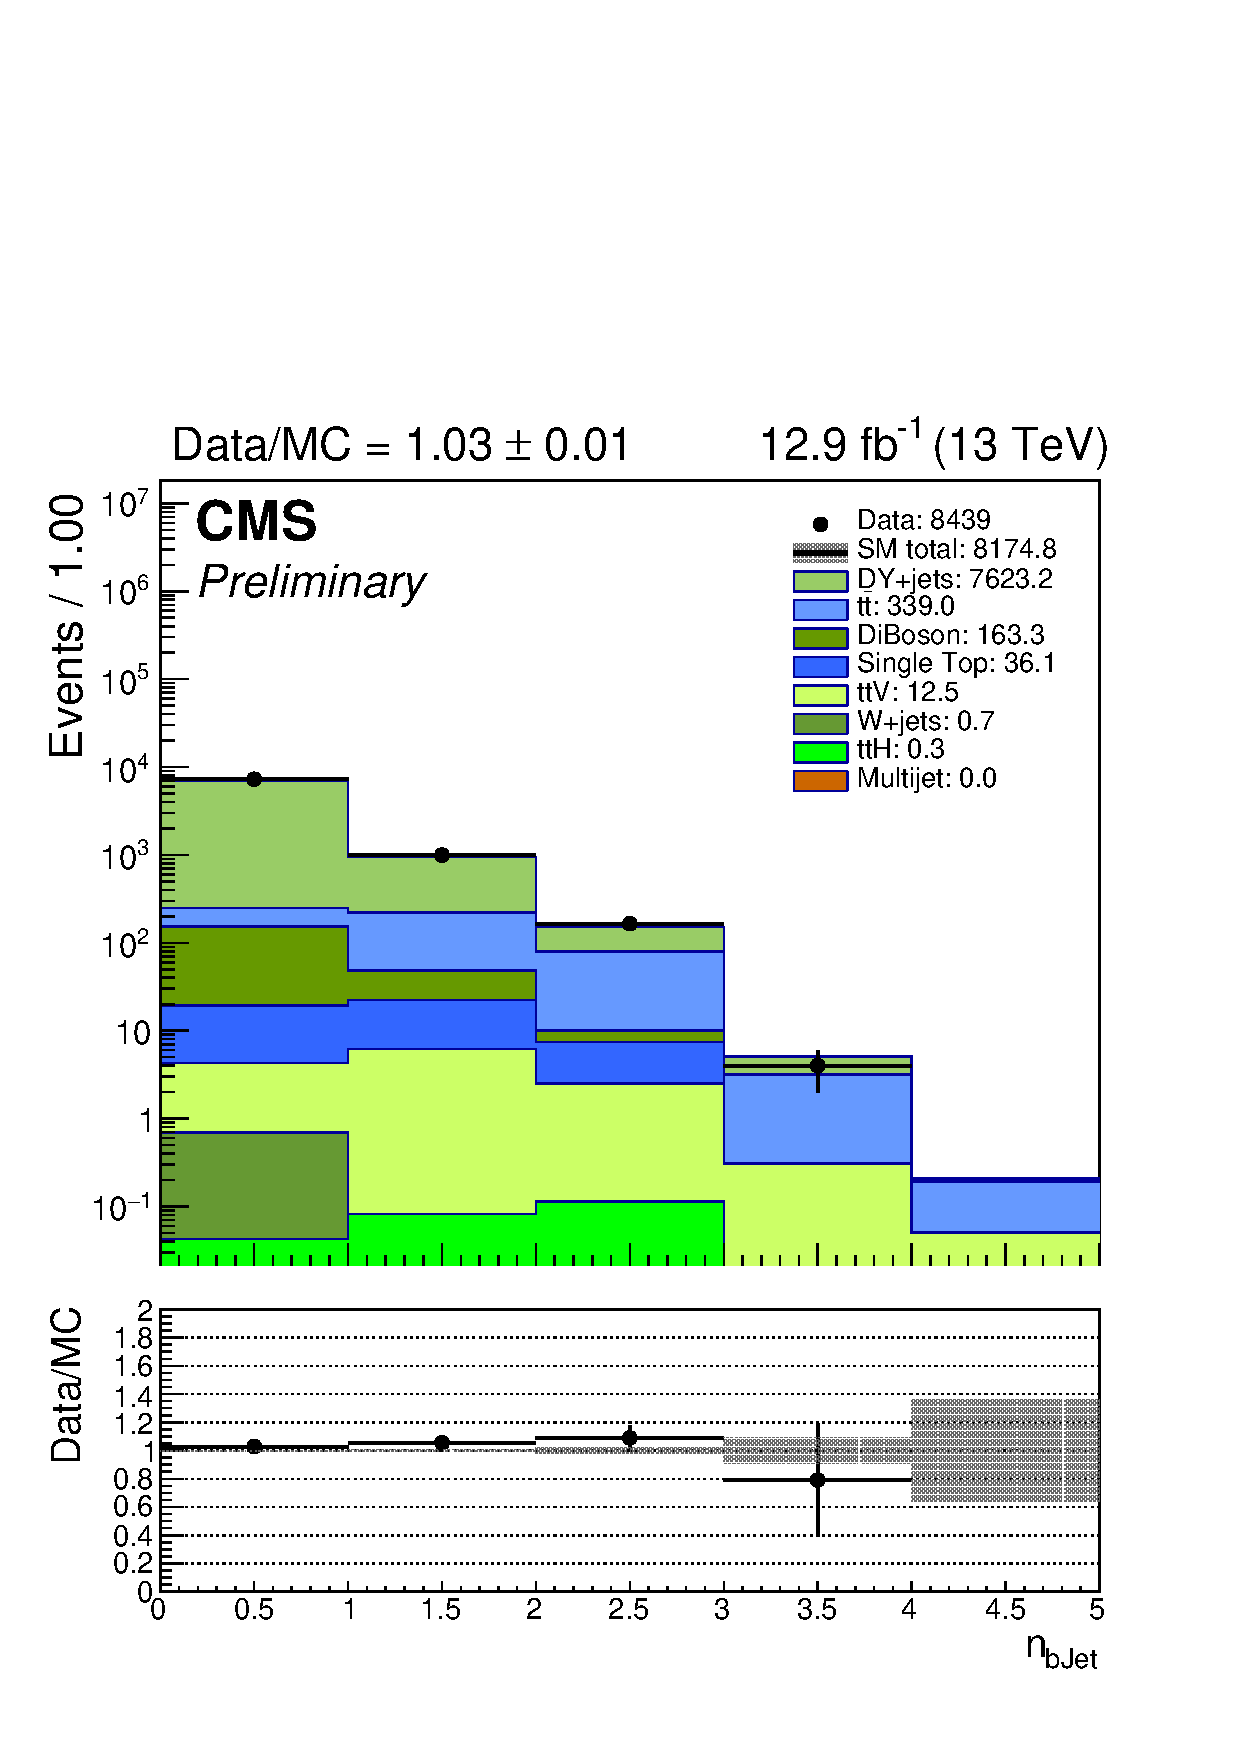
\includegraphics[width=0.5\textwidth]{figs/analysis/distributions/DoubleMu/nBJet40_asym.pdf}} \\
        \caption{Key analysis variables for double muon control region (asymmetric \njet bins)}
        \label{fig:distribution_doublemu_asym}
    \end{center}
\end{figure}

\begin{figure}
    \begin{center} 
        \subfloat {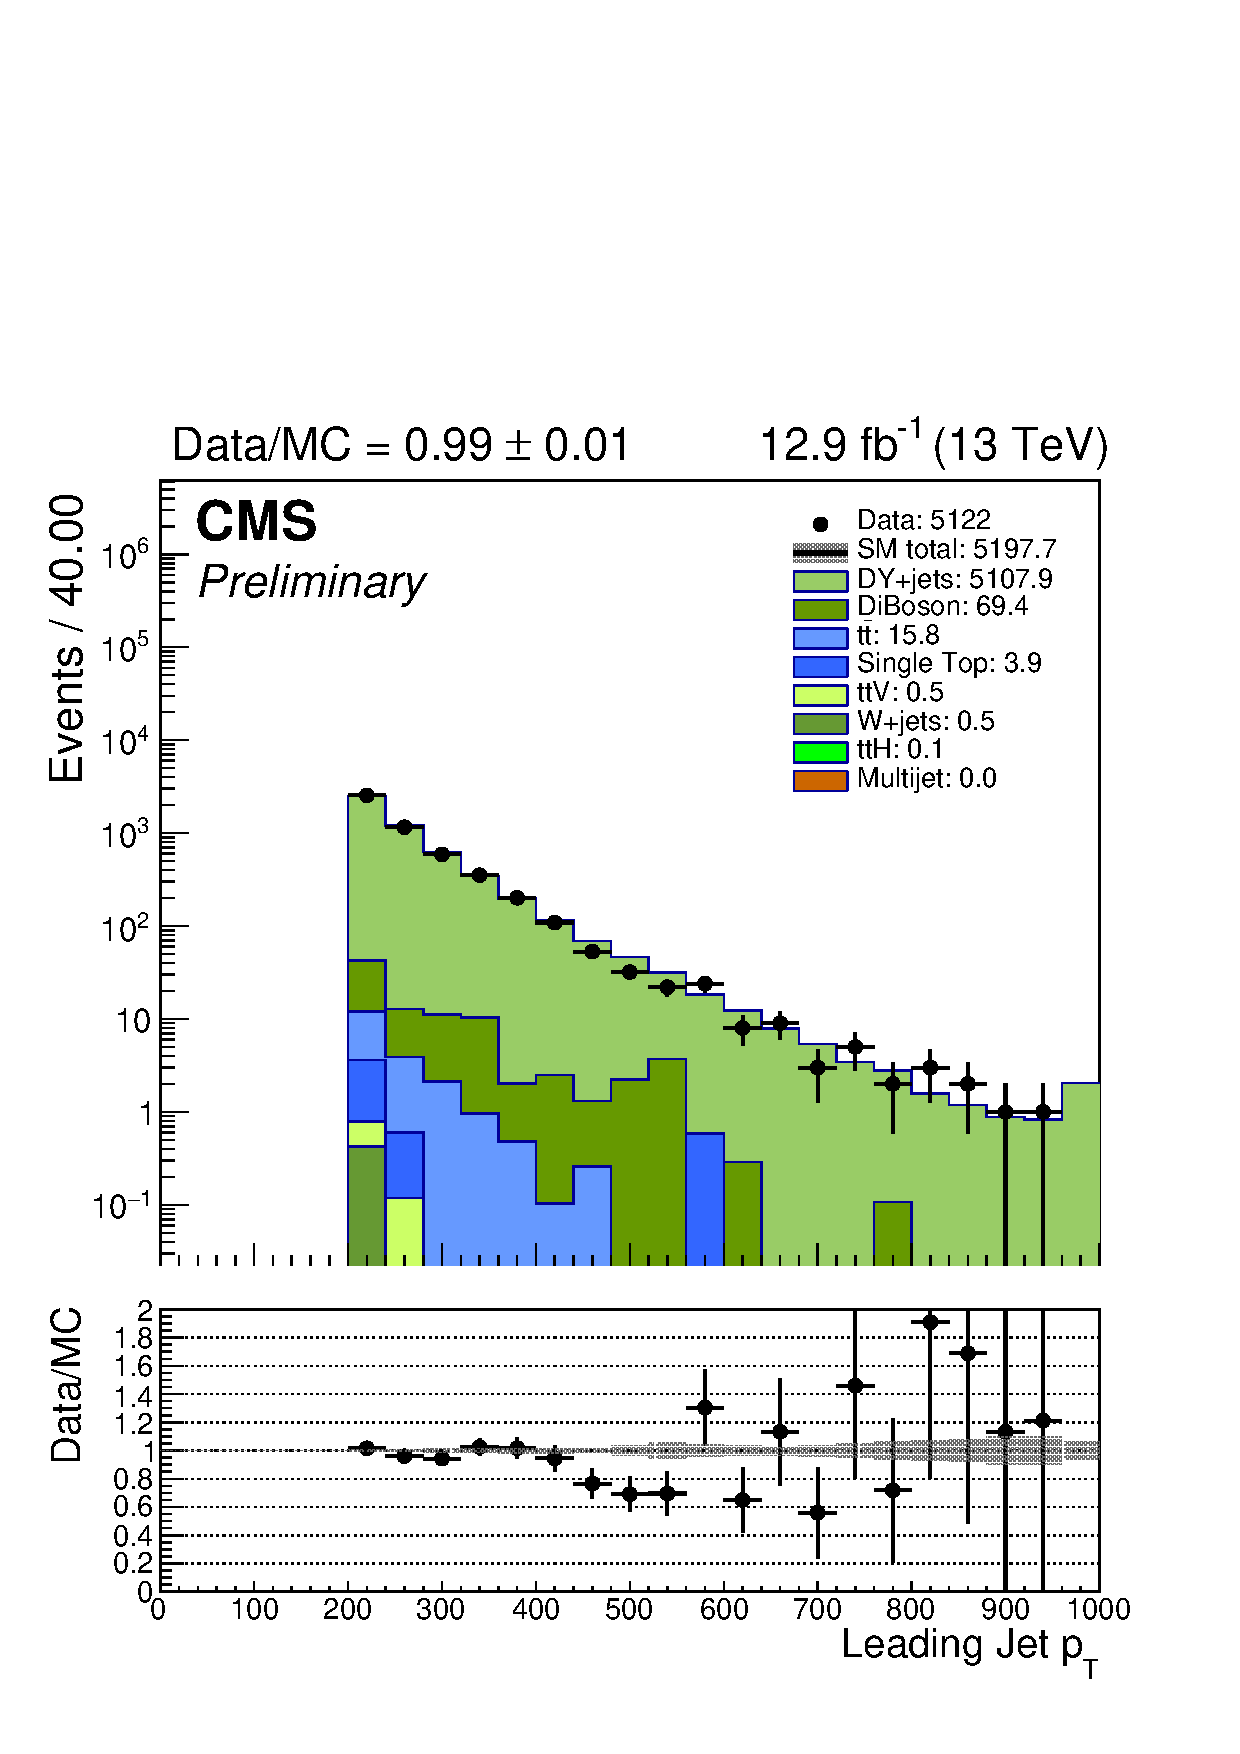
\includegraphics[width=0.5\textwidth]{figs/analysis/distributions/DoubleMu/jet_pt[0]_eq1j.pdf}} ~~
        \subfloat {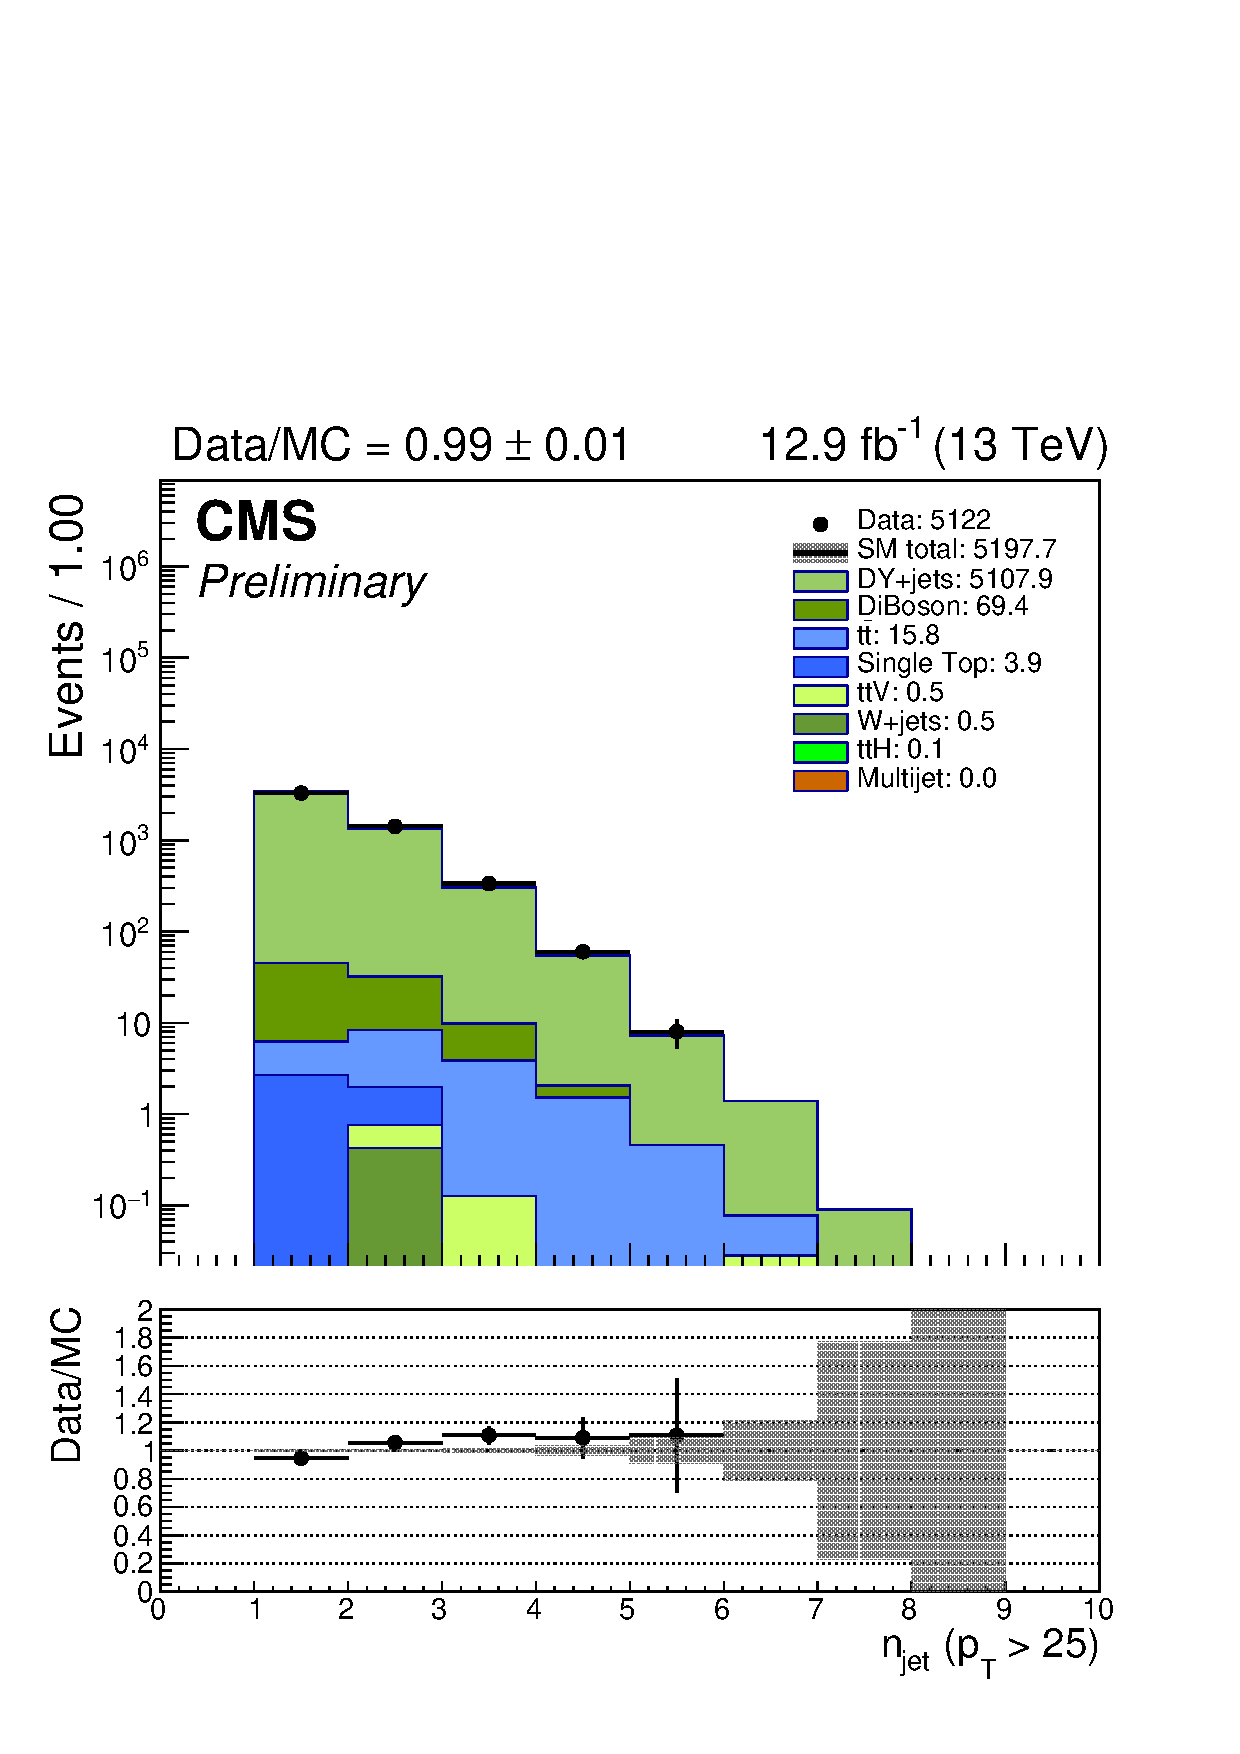
\includegraphics[width=0.5\textwidth]{figs/analysis/distributions/DoubleMu/njetInc_eq1j.pdf}} \\
        \subfloat {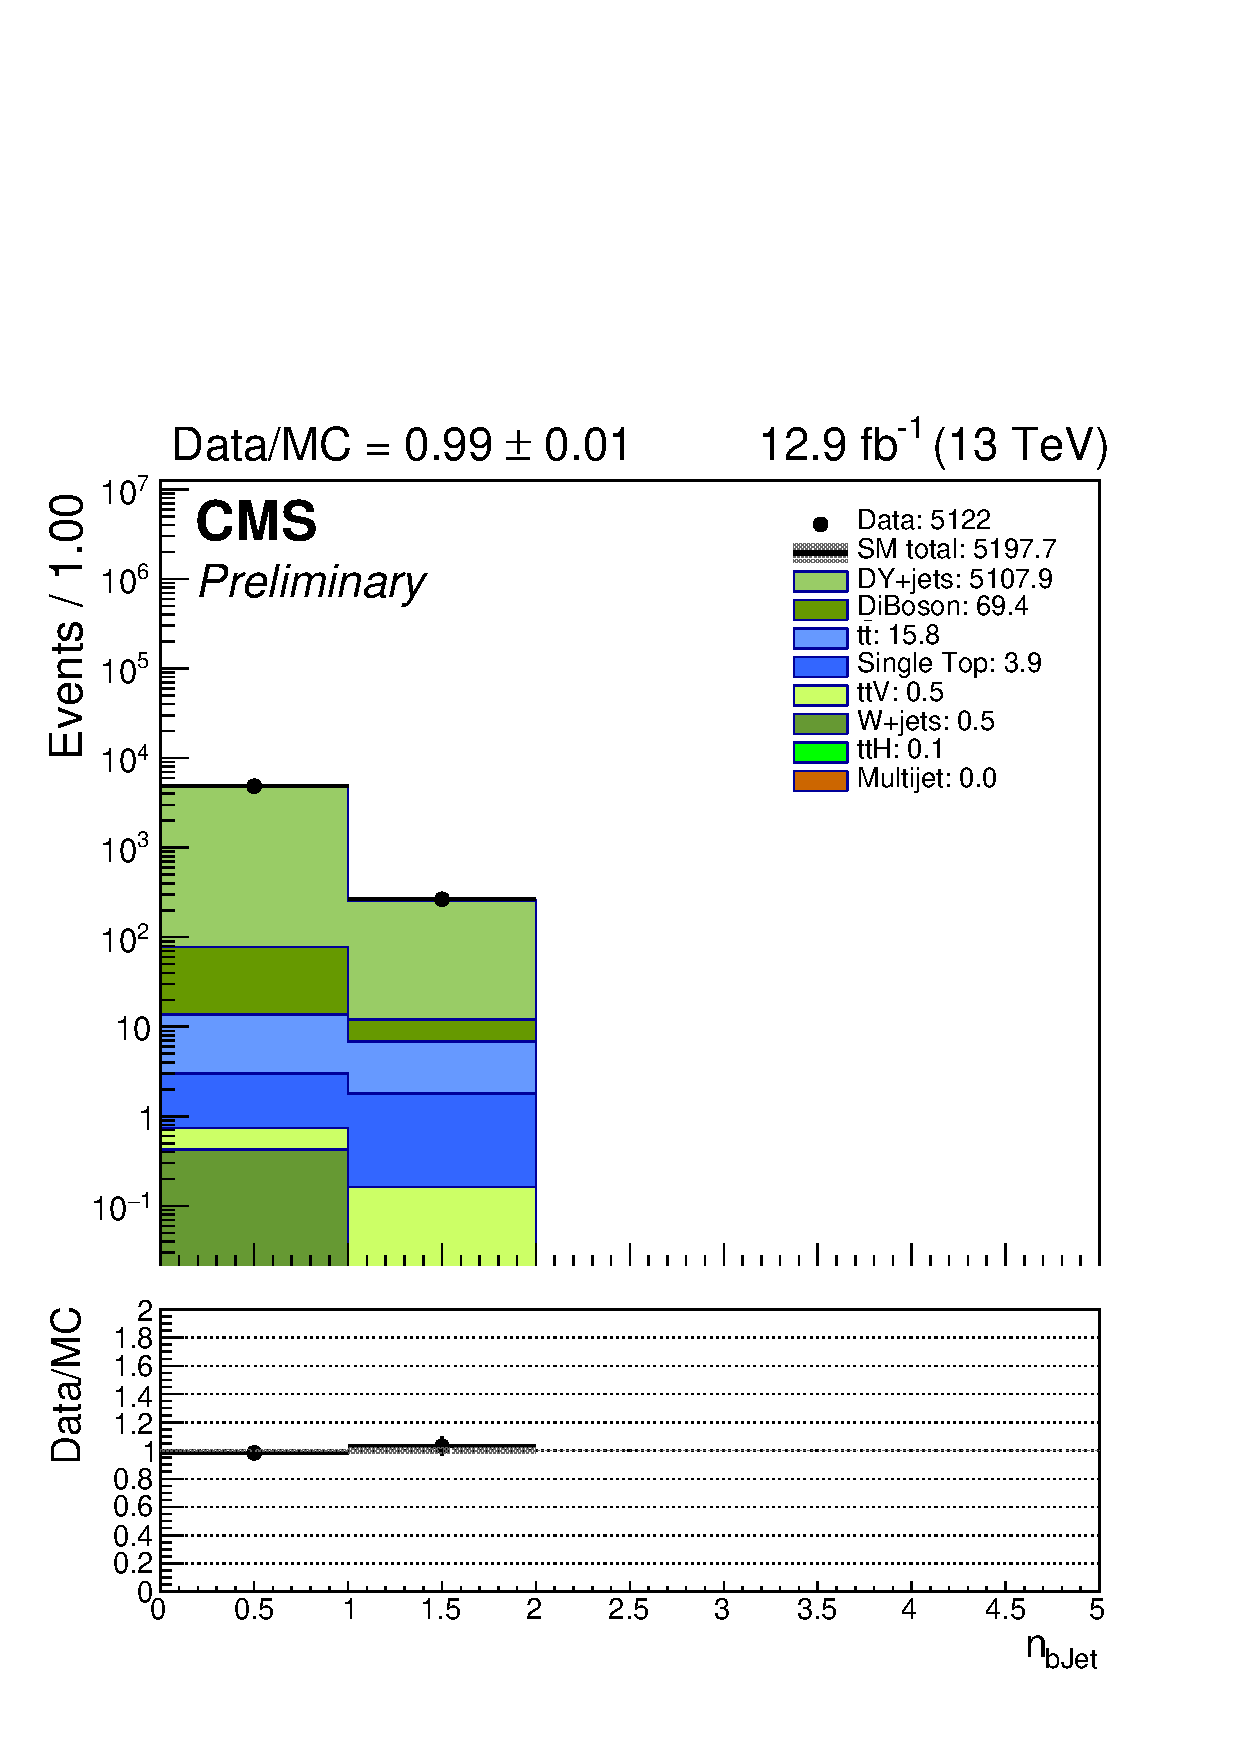
\includegraphics[width=0.5\textwidth]{figs/analysis/distributions/DoubleMu/nBJet40_eq1j.pdf}} ~~
        \subfloat {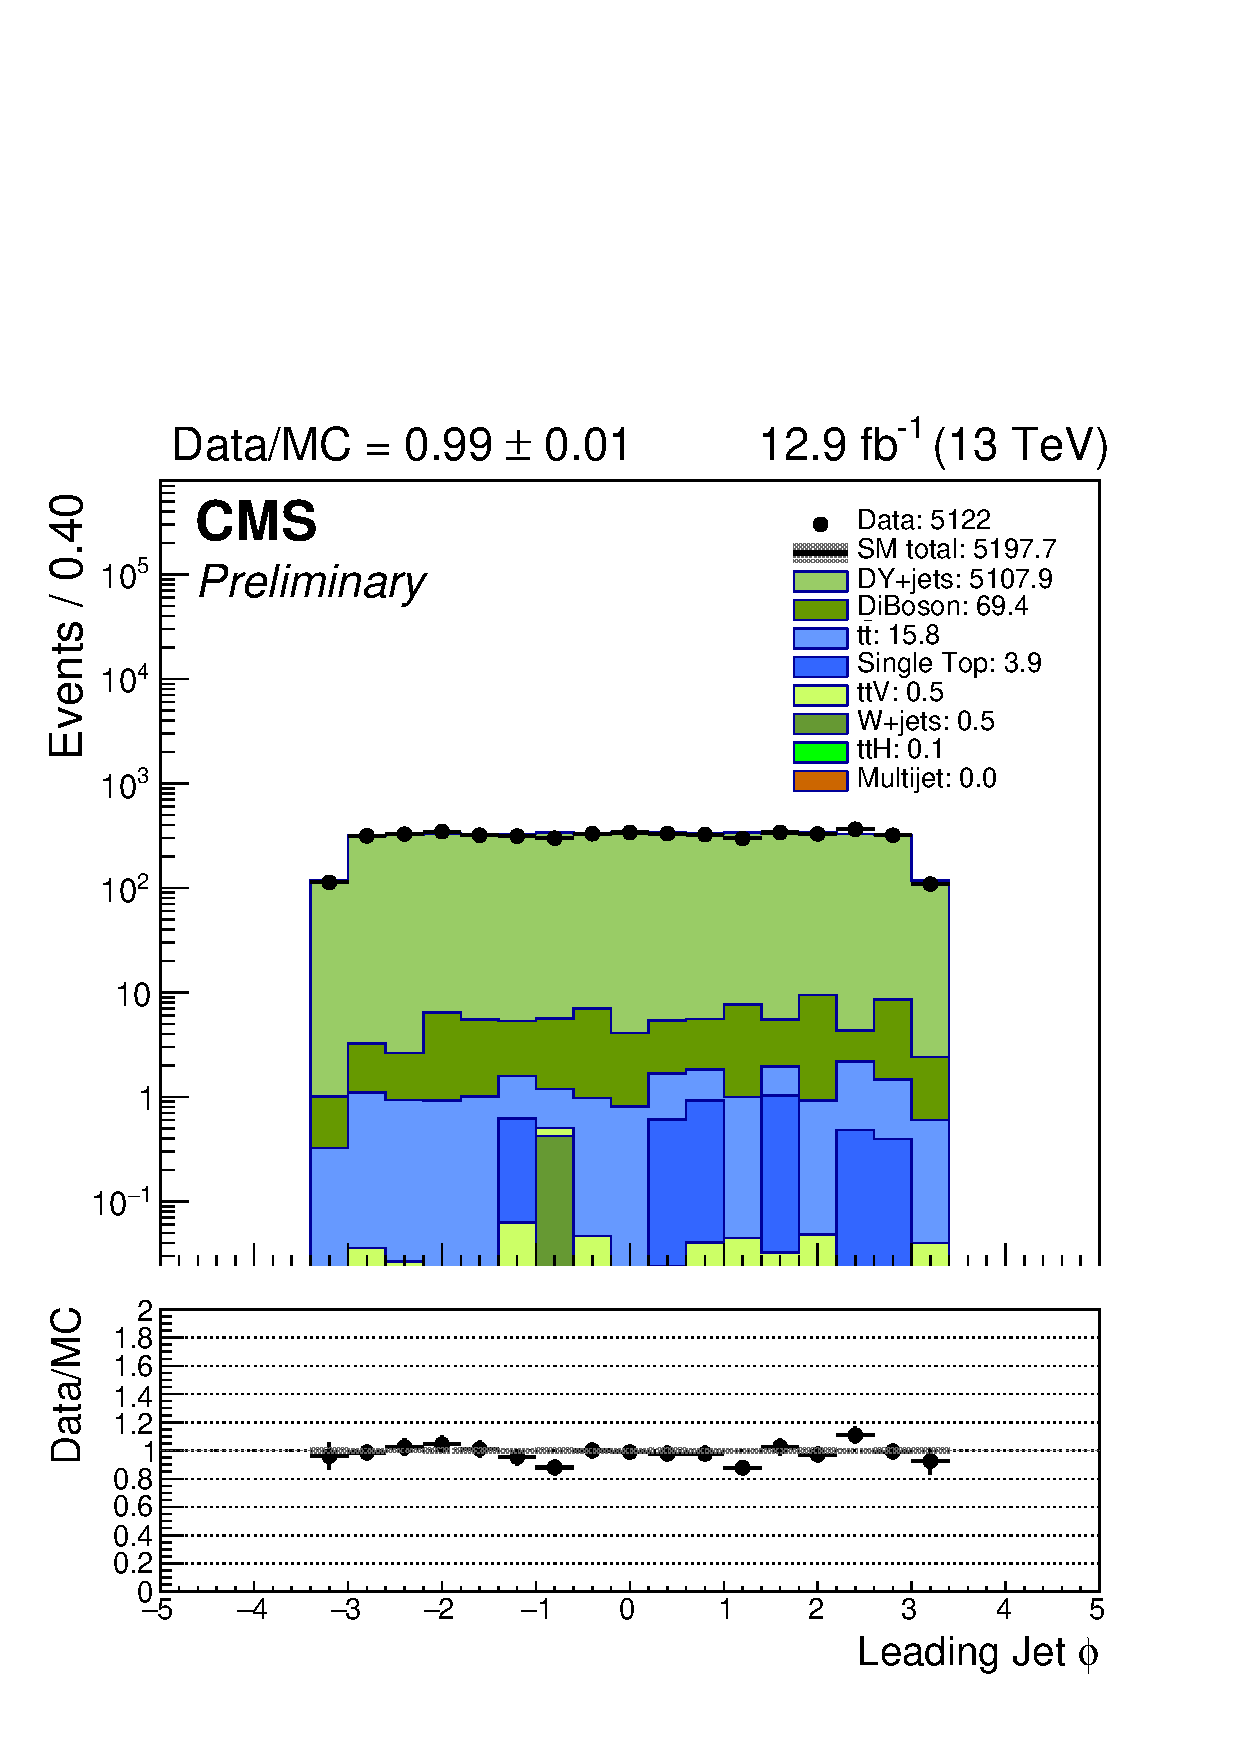
\includegraphics[width=0.5\textwidth]{figs/analysis/distributions/DoubleMu/jet_phi[0]_eq1j.pdf}} \\
        \caption{Key analysis variables for double muon control region (monojet bins)}
        \label{fig:distribution_doublemu_mono}
    \end{center}
\end{figure}

% \clearpage
% \subsection{Yields and distributions for the photon + jets control sample}

\begin{figure}
    \begin{center}
        \subfloat {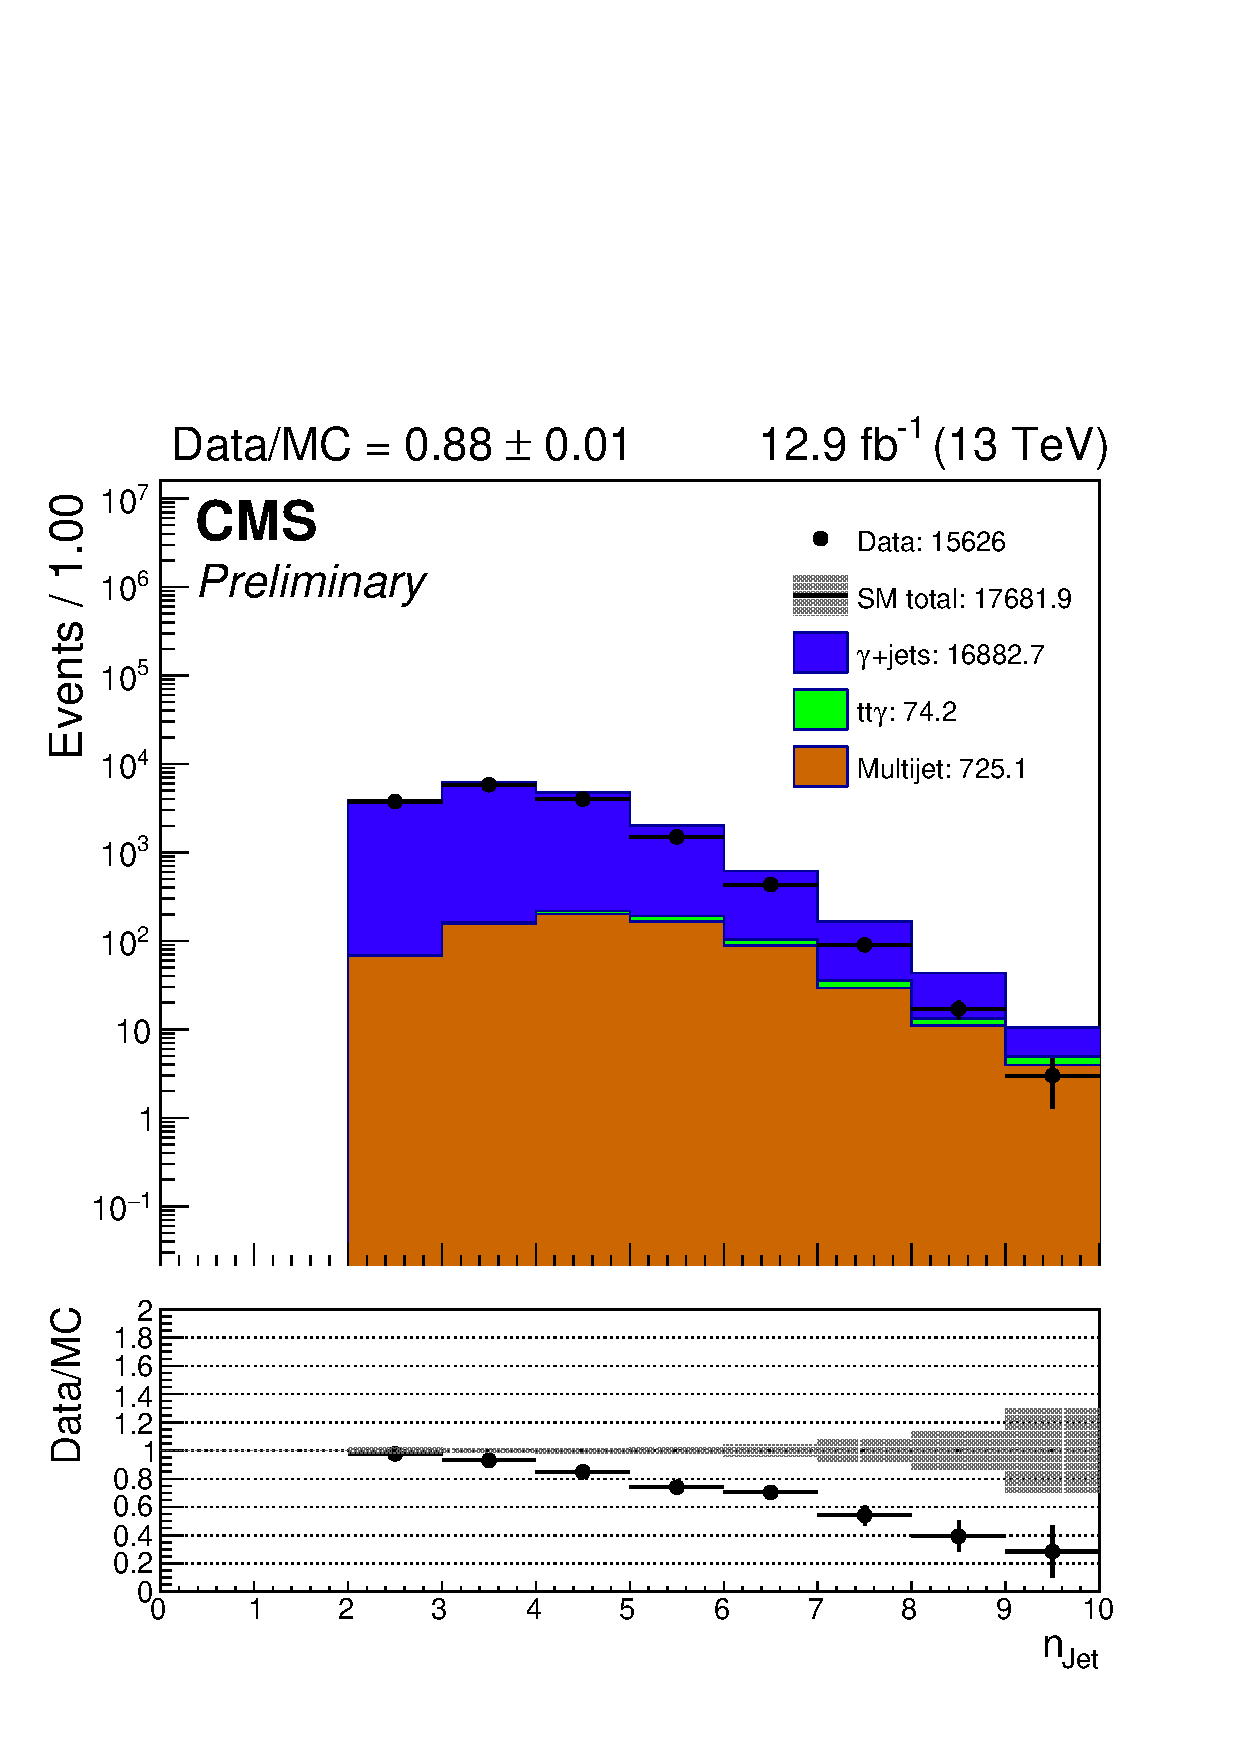
\includegraphics[width=0.5\textwidth]{figs/analysis/distributions/SinglePhoton/nJet40_sym.pdf}} ~~
        \subfloat {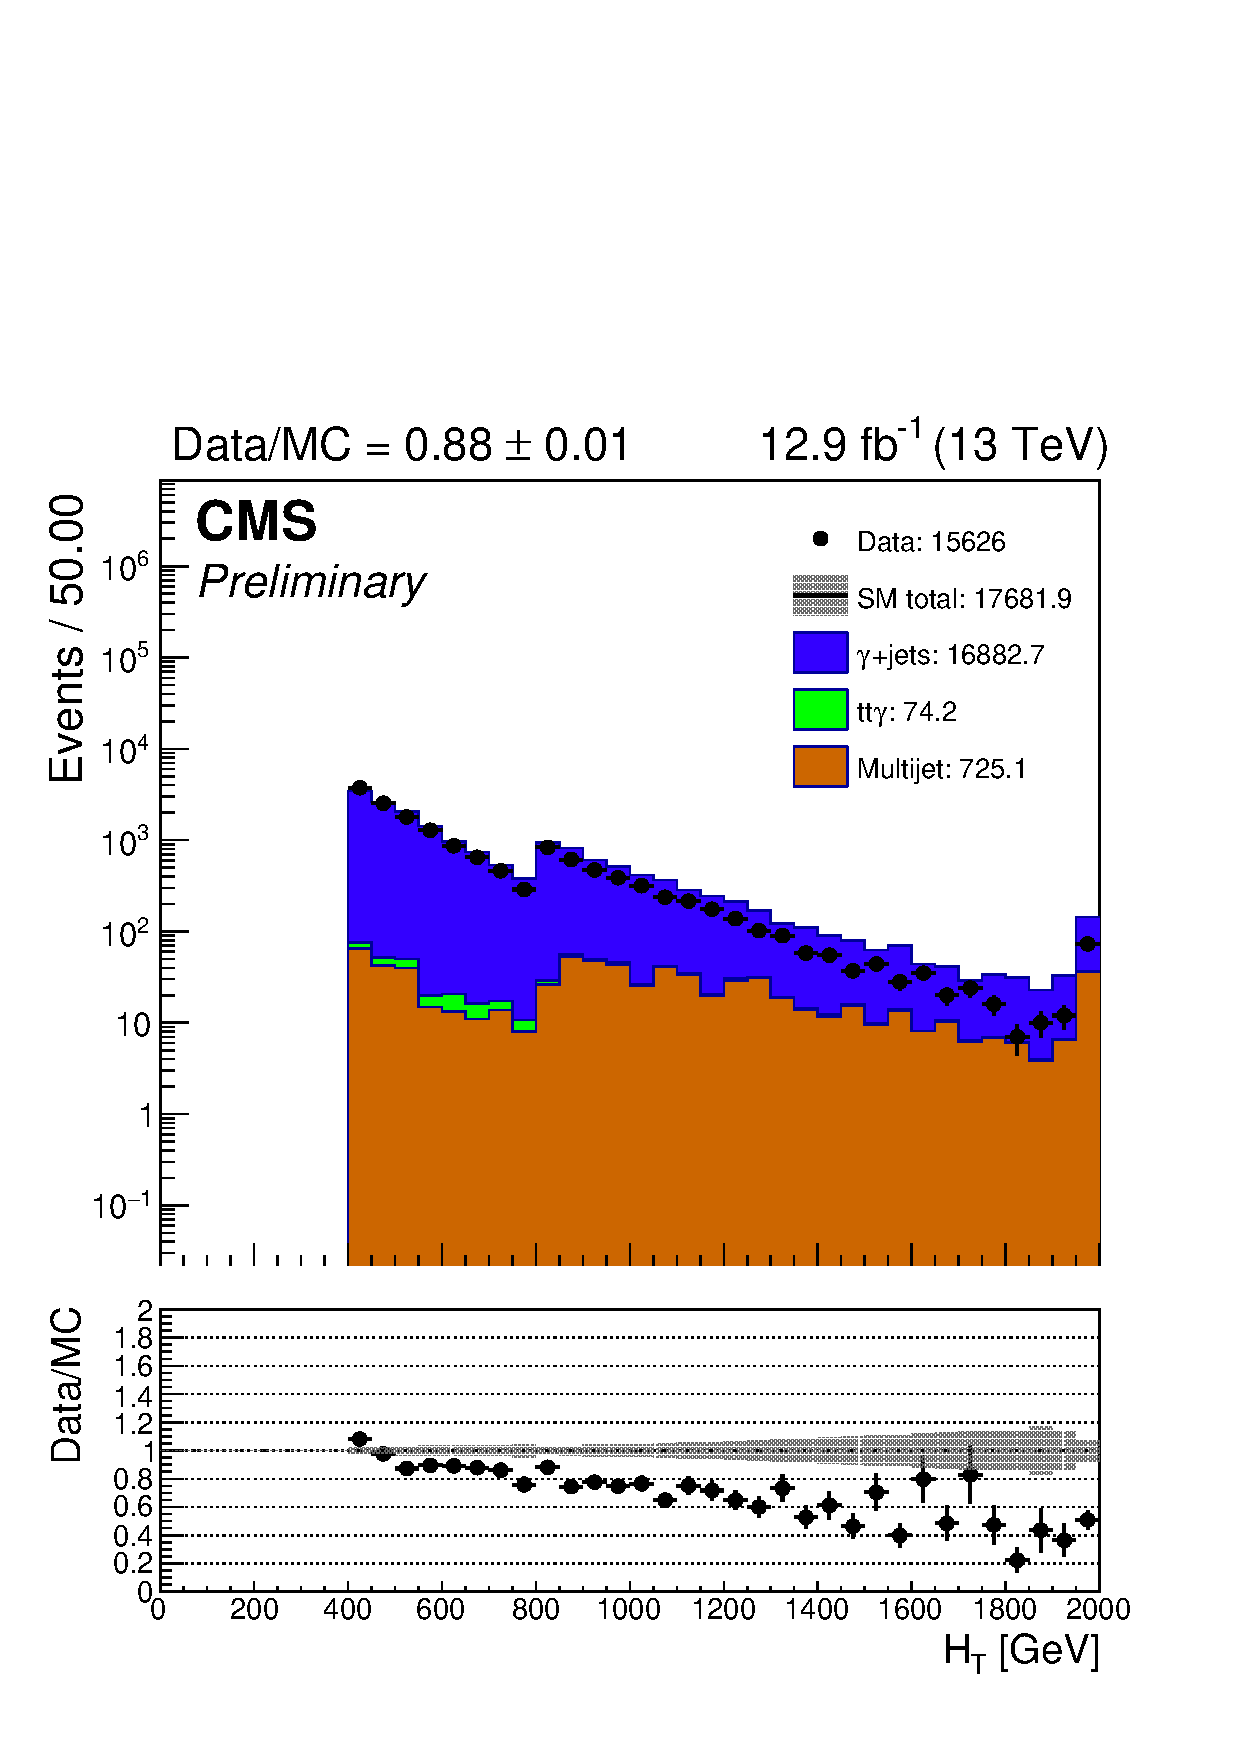
\includegraphics[width=0.5\textwidth]{figs/analysis/distributions/SinglePhoton/ht40_sym.pdf}} \\
        \subfloat {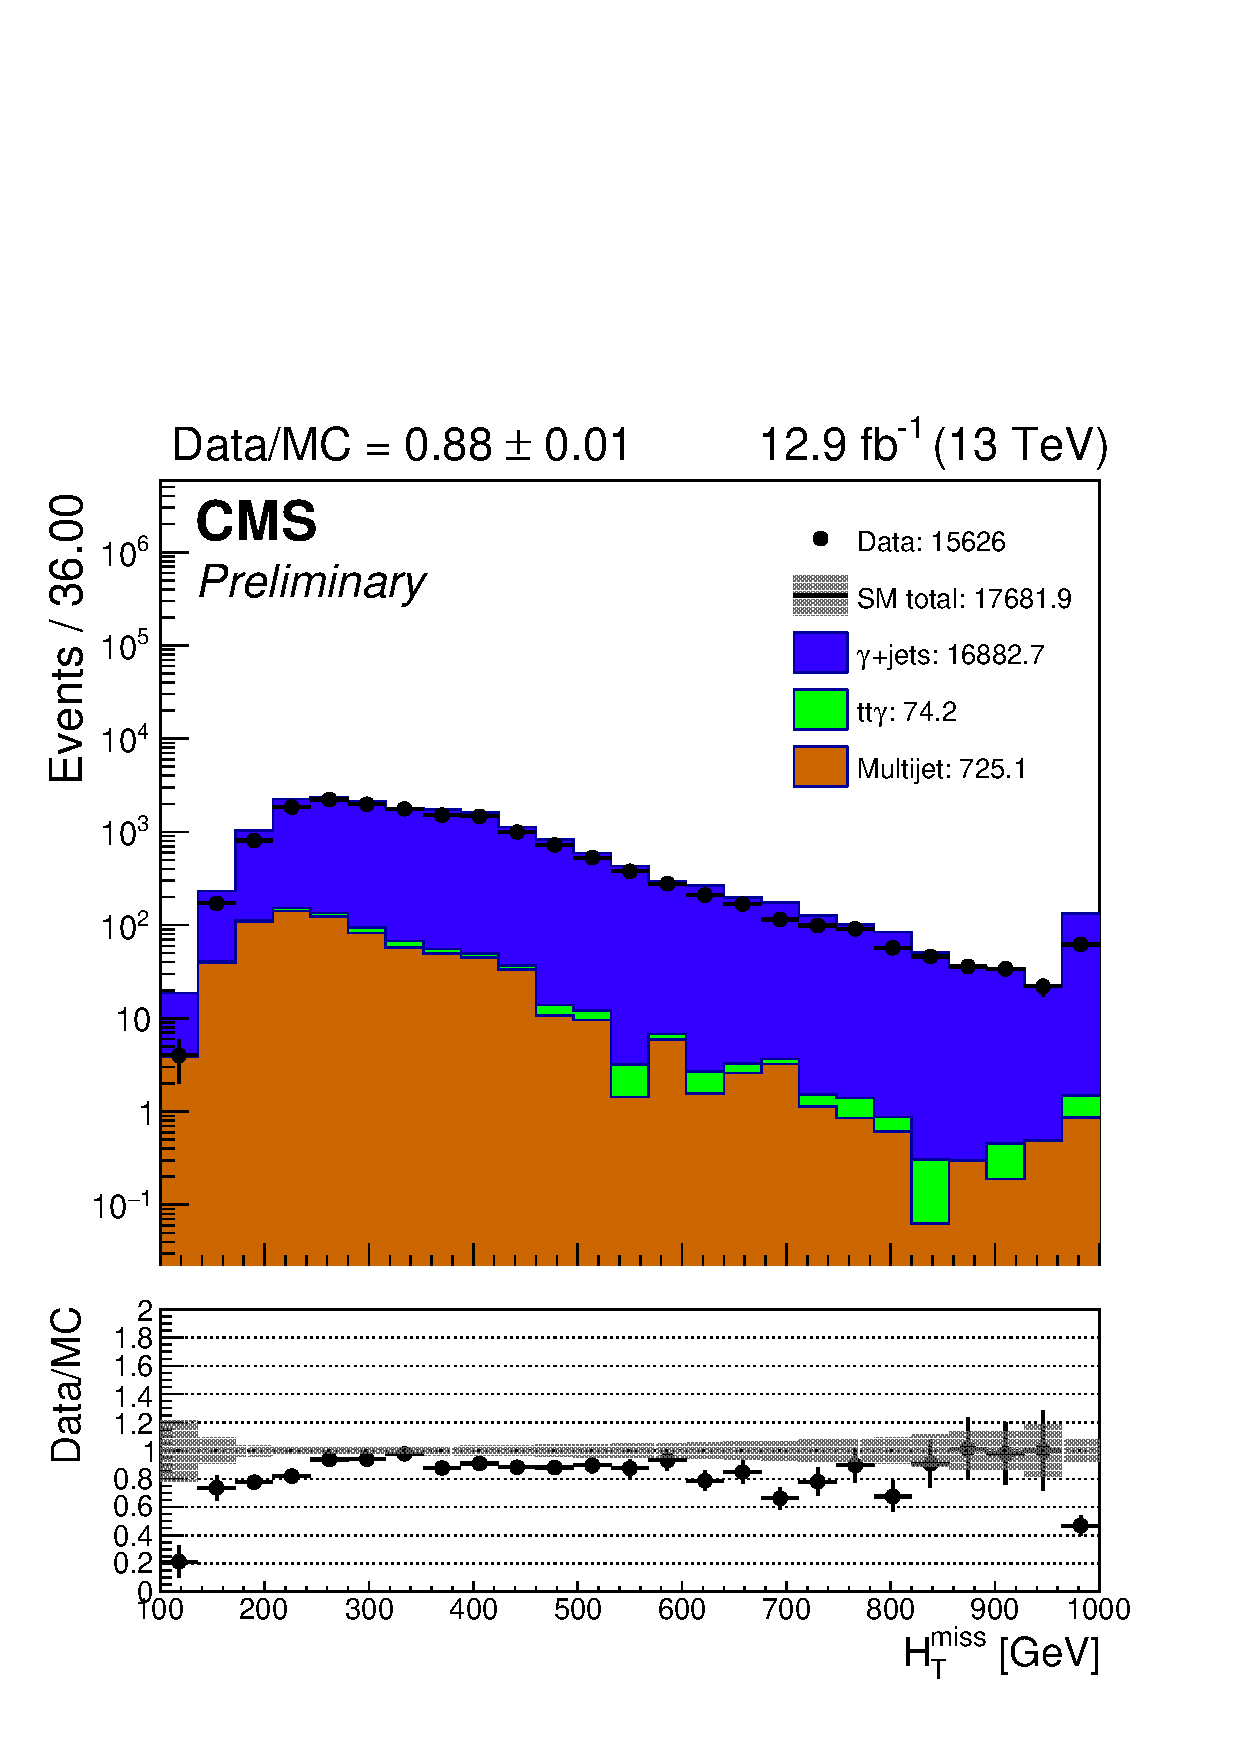
\includegraphics[width=0.5\textwidth]{figs/analysis/distributions/SinglePhoton/mht40_pt_sym.pdf}} ~~
        \subfloat {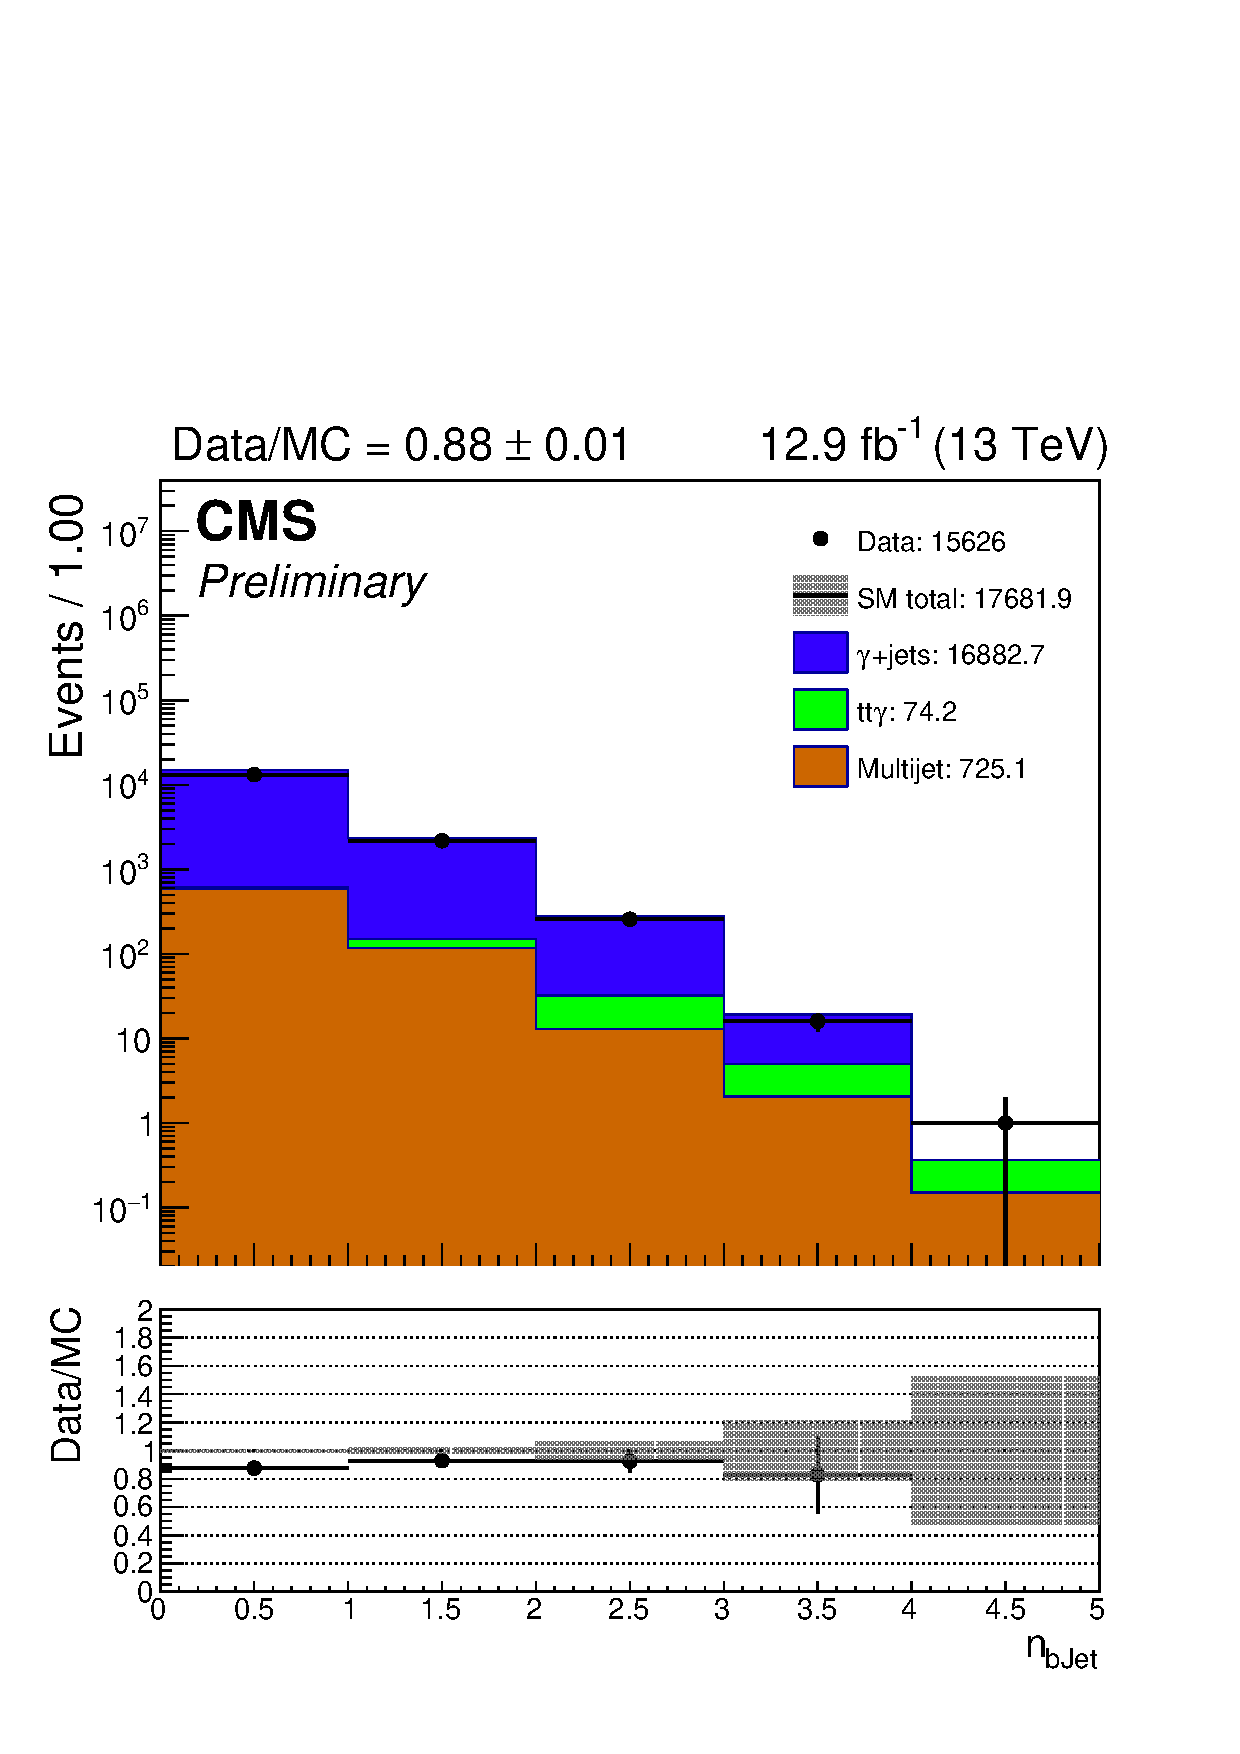
\includegraphics[width=0.5\textwidth]{figs/analysis/distributions/SinglePhoton/nBJet40_sym.pdf}} \\
        \caption{Key analysis variables for single photon control region (symmetric \njet bins)}
        \label{fig:distribution_singlephoton_sym}
    \end{center}
\end{figure}

\clearpage
\begin{figure}[h]
    \begin{center}
        \subfloat {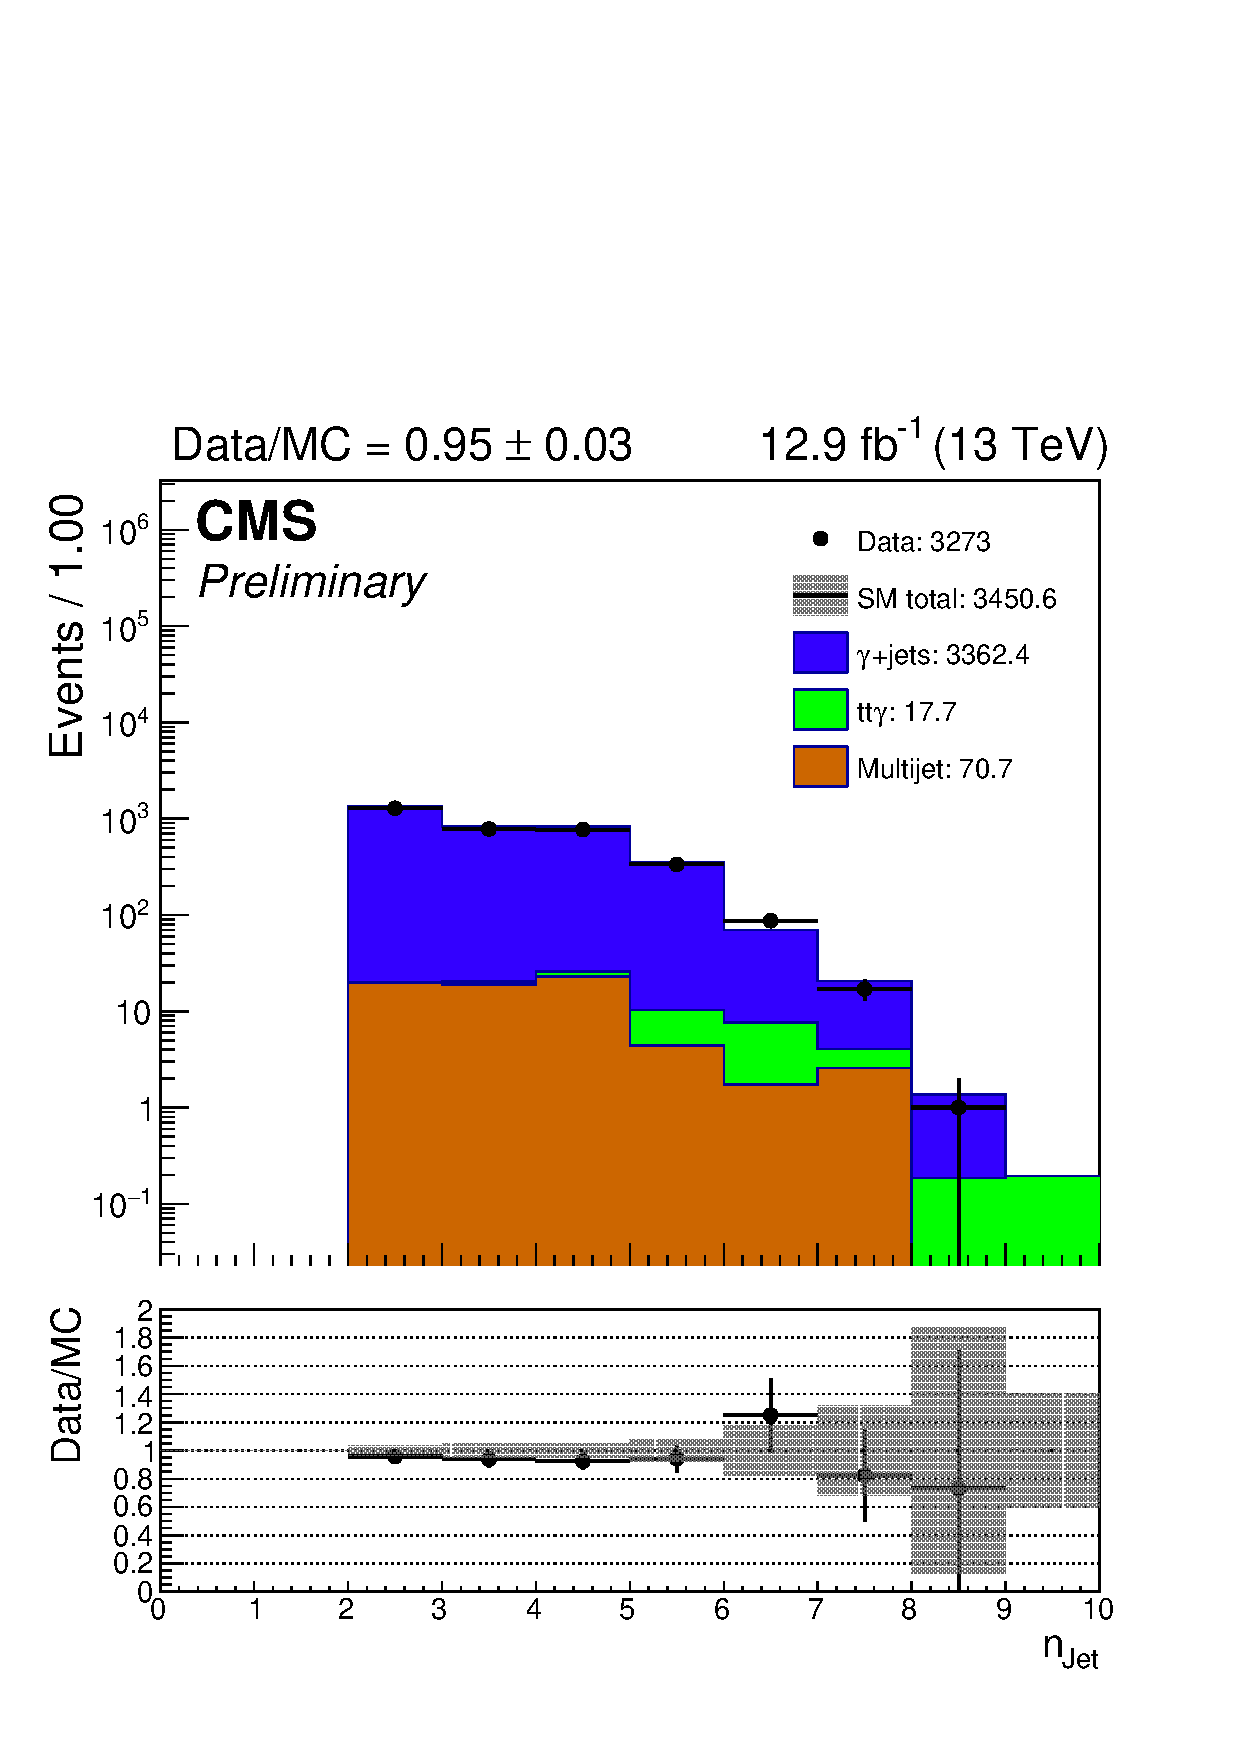
\includegraphics[width=0.5\textwidth]{figs/analysis/distributions/SinglePhoton/nJet40_asym.pdf}} ~~
        \subfloat {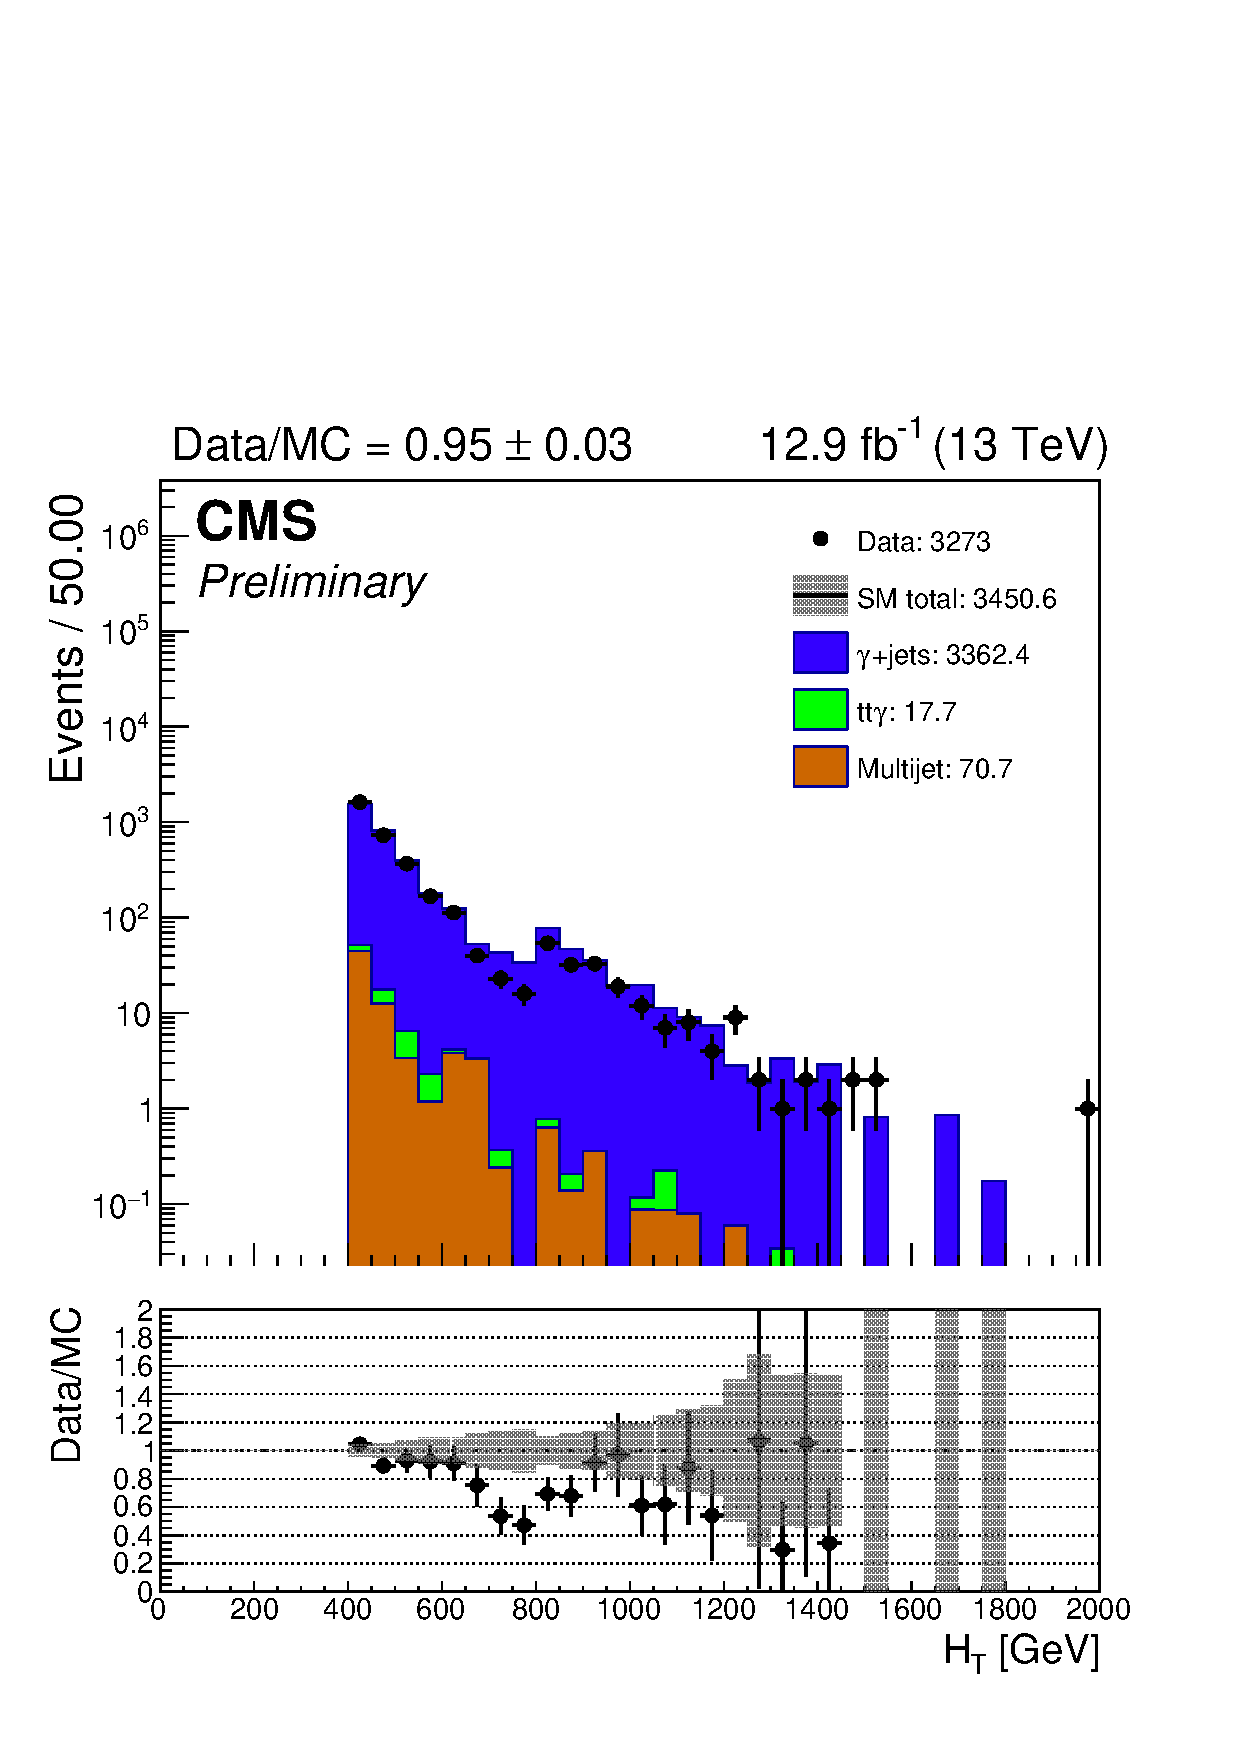
\includegraphics[width=0.5\textwidth]{figs/analysis/distributions/SinglePhoton/ht40_asym.pdf}} \\
        \subfloat {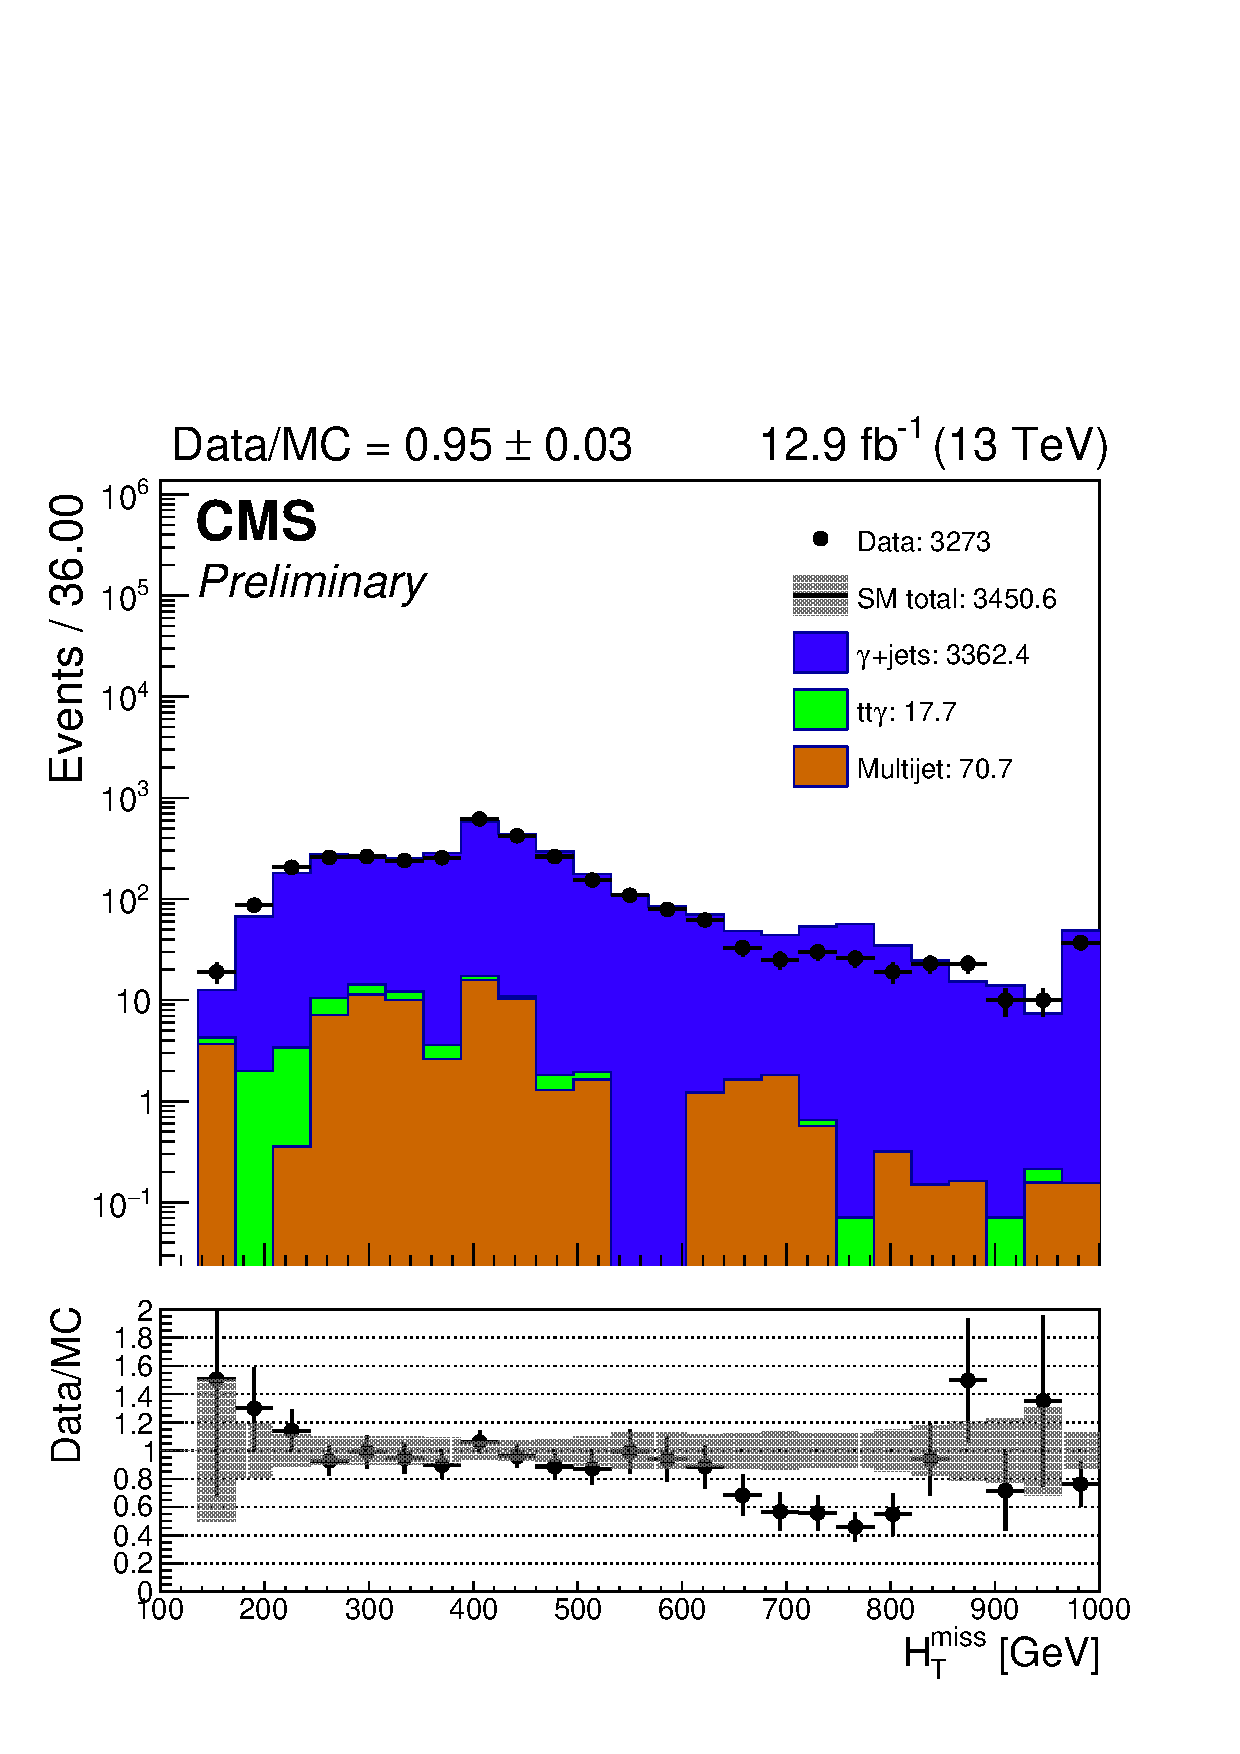
\includegraphics[width=0.5\textwidth]{figs/analysis/distributions/SinglePhoton/mht40_pt_asym.pdf}} ~~
        \subfloat {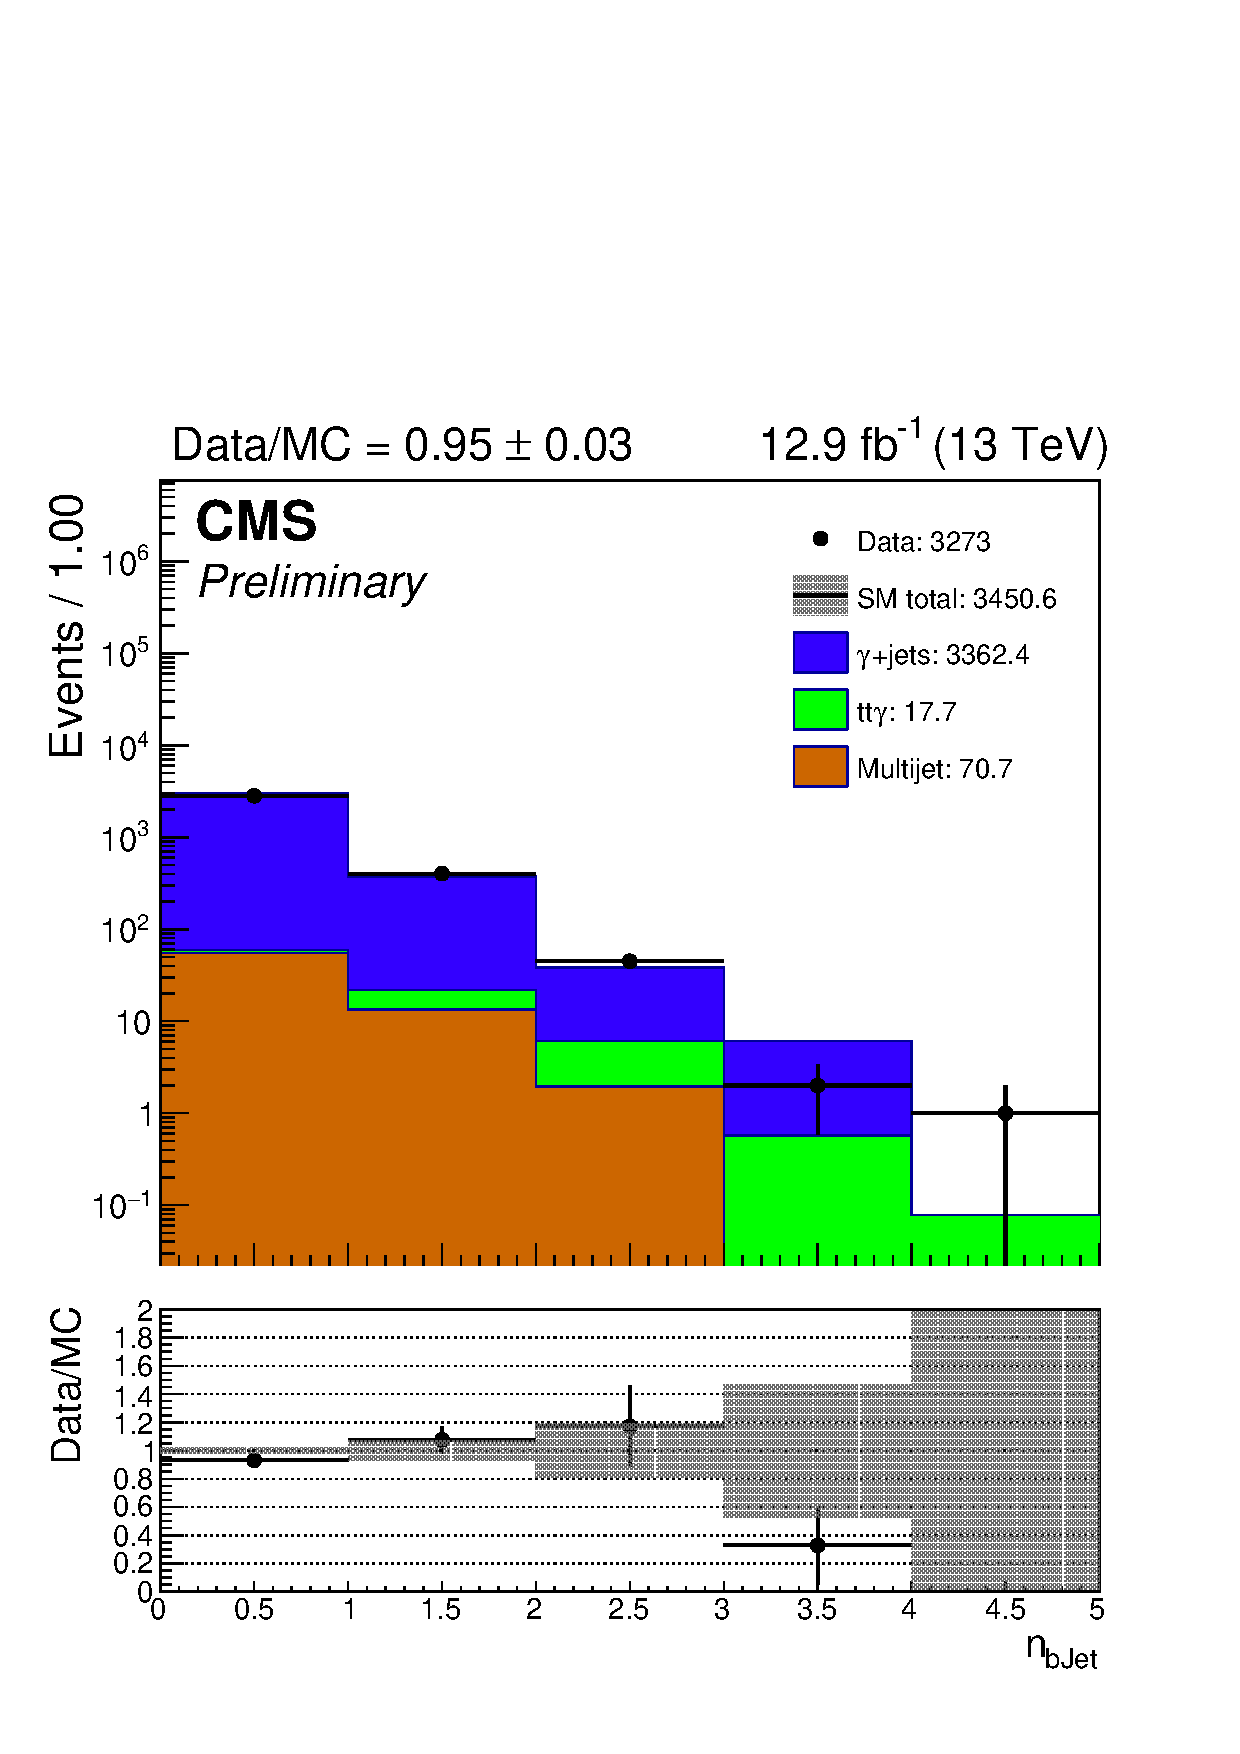
\includegraphics[width=0.5\textwidth]{figs/analysis/distributions/SinglePhoton/nBJet40_asym.pdf}} \\
        \caption{Key analysis variables for single photon control region (asymmetric \njet bins)}
        \label{fig:distribution_singlephoton_asym}
    \end{center}
\end{figure}

\clearpage
\begin{figure}
    \begin{center} 
        \subfloat {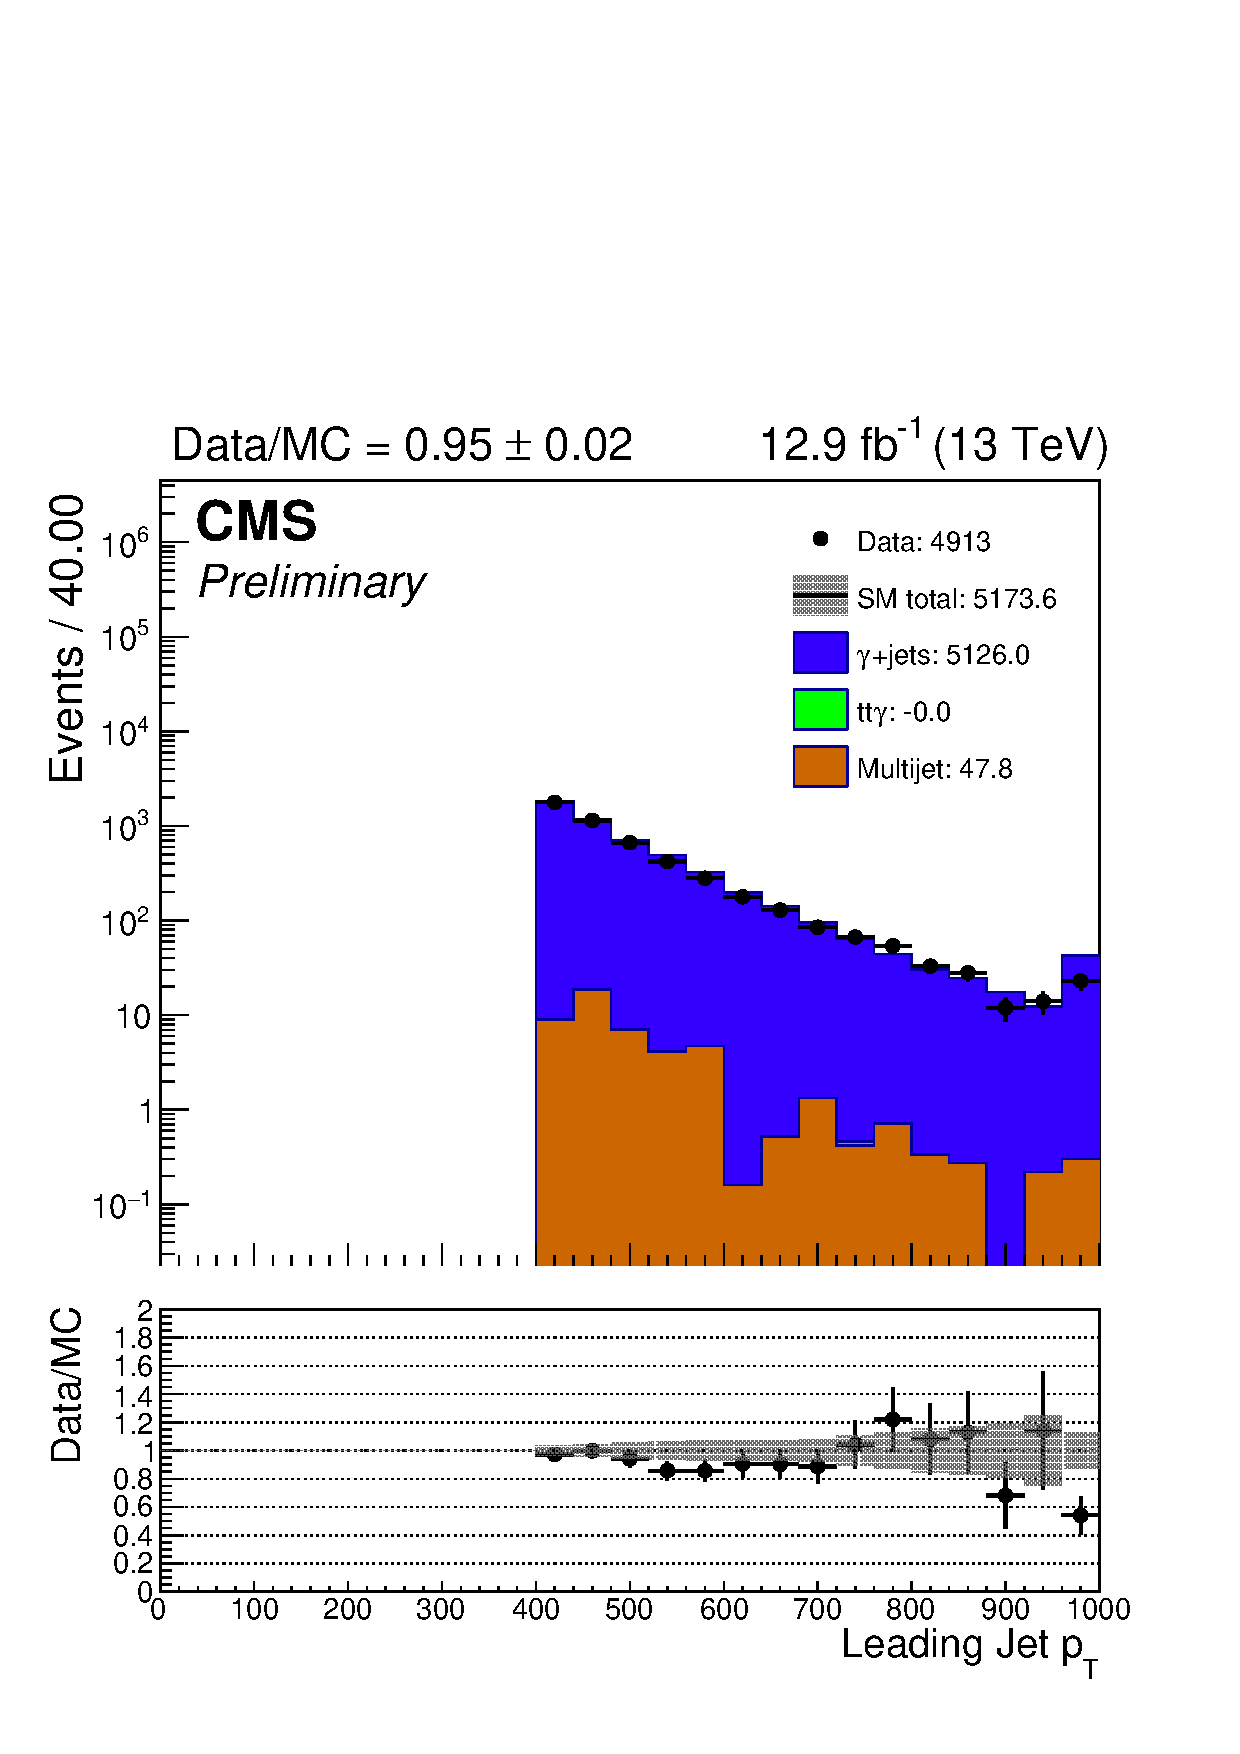
\includegraphics[width=0.5\textwidth]{figs/analysis/distributions/SinglePhoton/jet_pt[0]_eq1j.pdf}} ~~
        \subfloat {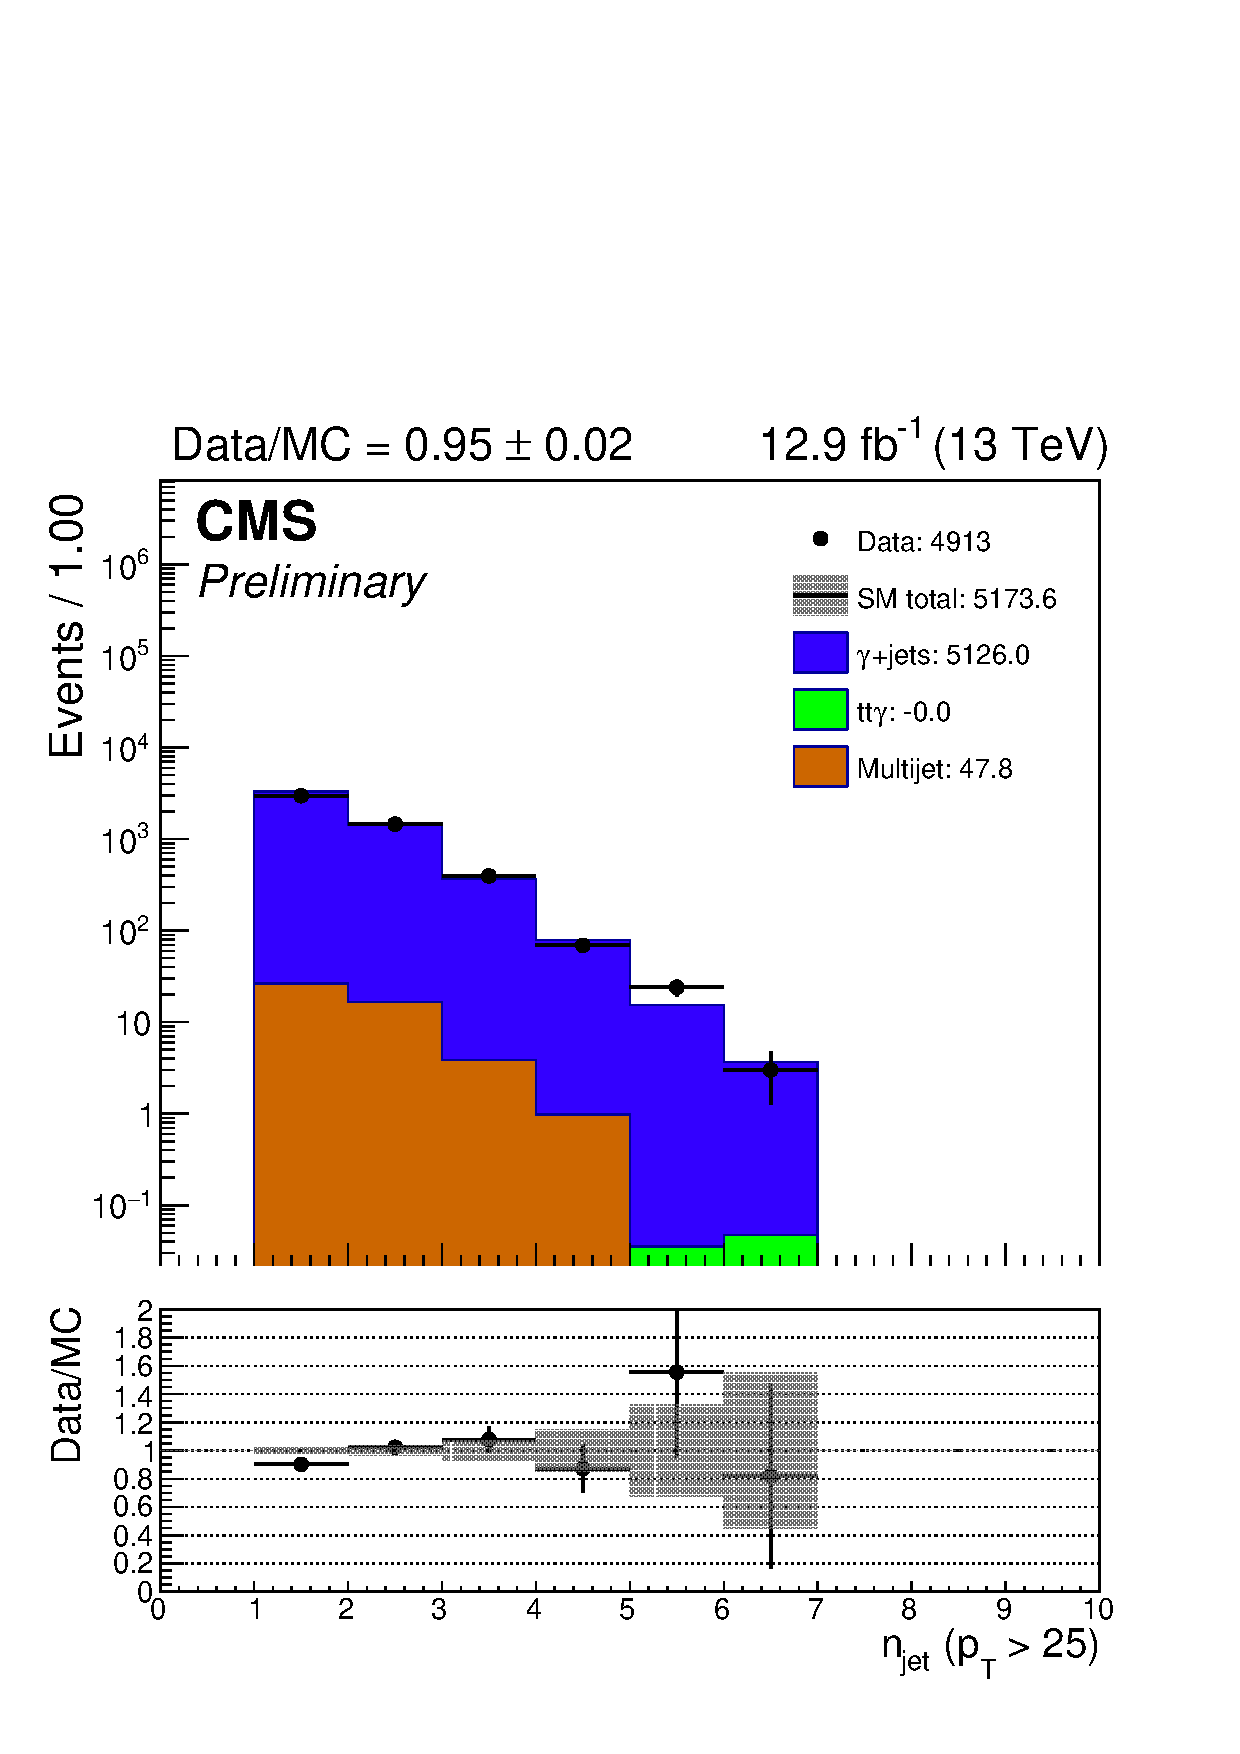
\includegraphics[width=0.5\textwidth]{figs/analysis/distributions/SinglePhoton/njetInc_eq1j.pdf}} \\
        \subfloat {\includegraphics[width=0.5\textwidth]{figs/analysis/distributions/SinglePhoton/nBJet40_eq1j.pdf}} ~~
        \subfloat {\includegraphics[width=0.5\textwidth]{figs/analysis/distributions/SinglePhoton/jet_phi[0]_eq1j.pdf}} \\
        \caption{Key analysis variables for single photon control region (monojet bins)}
        \label{fig:distribution_singlephoton_mono}
    \end{center}
\end{figure}

% \clearpage
% \subsection{Expected yields and distributions in the signal region}
\clearpage
\begin{figure}
    \begin{center}
        \subfloat {\includegraphics[width=0.5\textwidth]{figs/analysis/distributions/Signal/jet_pt[0]_eq1j.pdf}} ~~
        \subfloat {\includegraphics[width=0.5\textwidth]{figs/analysis/distributions/Signal/njetInc_eq1j.pdf}} \\
        \subfloat {\includegraphics[width=0.5\textwidth]{figs/analysis/distributions/Signal/nBJet40_eq1j.pdf}} ~~
        \subfloat {\includegraphics[width=0.5\textwidth]{figs/analysis/distributions/Signal/jet_phi[0]_eq1j.pdf}} \\
        \caption{Key analysis variables for hadronic signal region (monojet bins)}
        \label{fig:distribution_signal_mono}
    \end{center}
\end{figure}

\clearpage
\section{Binning of \MHT dimension}
\label{app:mhtBinning} 
In Tab. \ref{tab:mhtBins_eq2j}-\ref{tab:mhtBins_ge5a} the binning of
the \mht dimension for all the categories used in the analysis is
presented, for the asymmetric and symmetric topologies respectively.
Where the binning is not specified no template is used.  For the
monojet category no template is used. 

\begin{table}[h!]
  \scriptsize
  \centering
  \caption{The \mht binning for the jet category $n_{jet} = 2$. 
  \label{tab:mhtBins_eq2j}}
  \begin{tabular}{ lll }
    Jet category & $H_{T}$ bin & \mht template binning (GeV) \\ \hline

    \hline
    $\njet = 2 \;, \nb = 0 $ & $200 < H_{T} < 250$ GeV & 130, 175, 225 \\ 
     & $250 < H_{T} < 300$ GeV & 130, 175, 225, 275 \\ 
     & $300 < H_{T} < 350$ GeV & 130, 175, 225, 275, 325 \\ 
     & $350 < H_{T} < 400$ GeV & 130, 175, 225, 275, 325, 375 \\ 
     & $400 < H_{T} < 500$ GeV & 130, 175, 225, 275, 325, 375, 425, 475 \\ 
     & $500 < H_{T} < 600$ GeV & 130, 175, 225, 275, 325, 375, 425, 475, 525, 575 \\ 
     & $600 < H_{T} < 800$ GeV & 130, 175, 225, 275, 325, 375, 425, 475, 525, 575, 625, 675, 725, 775 \\ 
     & $H_{T} > 800$ GeV & 130, 250, 300, 350, 400, 450, 500, 550, 600, 650, 700, 750, 800 \\ 
    \hline
    $\njet = 2 \;, \nb = 1$ & $200 < H_{T} < 250$ GeV & 130, 175, 225 \\ 
     & $250 < H_{T} < 300$ GeV & 130, 175, 225, 275 \\ 
     & $300 < H_{T} < 350$ GeV & 130, 175, 225, 275, 325 \\ 
     & $350 < H_{T} < 400$ GeV & 130, 175, 225, 275, 325, 375 \\ 
     & $400 < H_{T} < 500$ GeV & 130, 175, 225, 275, 325, 375, 425, 475 \\ 
     & $500 < H_{T} < 600$ GeV & 130, 225, 275, 325, 375, 425, 475, 525, 575 \\ 
     & $600 < H_{T} < 800$ GeV & 130, 225, 275, 325, 375, 425, 475, 525, 575, 675, 725, 775 \\ 
     & $H_{T} > 800$ GeV & 130, 250, 300, 350, 400, 450, 500, 550, 600, 650, 700, 750, 800 \\ 
    \hline
    $\njet = 2 \;, \nb = 2 $ & $200 < H_{T} < 250$ GeV & - \\ 
     & $250 < H_{T} < 300$ GeV & 130, 175, 225, 275 \\ 
     & $300 < H_{T} < 350$ GeV & - \\ 
     & $350 < H_{T} < 400$ GeV & 130, 250, 300, 350 \\ 
     & $400 < H_{T} < 500$ GeV & - \\ 
     & $500 < H_{T} < 600$ GeV & 130, 225, 325, 375, 475, 525, 575 \\ 
     & $H_{T} > 600$ GeV & - \\ 

  \end{tabular}
\end{table}



\begin{table}[h!]
  \scriptsize
  \centering
  \caption{The \mht binning for the jet category $n_{jet} = 3$. 
  \label{tab:mhtBins_eq3j}}
  \begin{tabular}{ lll }
    Jet category & $H_{T}$ bin & \mht template binning (GeV) \\ \hline

    \hline
    $\njet = 3 \;, \nb = 0 $ & $200 < H_{T} < 250$ GeV & 130, 225 \\ 
     & $250 < H_{T} < 300$ GeV & 130, 175, 225, 275 \\ 
     & $300 < H_{T} < 350$ GeV & 130, 175, 225, 275, 325 \\ 
     & $350 < H_{T} < 400$ GeV & 130, 175, 225, 275, 325, 375 \\ 
     & $400 < H_{T} < 500$ GeV & 130, 175, 225, 275, 325, 375, 425, 475 \\ 
     & $500 < H_{T} < 600$ GeV & 130, 175, 225, 275, 325, 375, 425, 475, 525, 575 \\ 
     & $600 < H_{T} < 800$ GeV & 130, 225, 275, 325, 375, 425, 475, 525, 575, 625, 675, 725, 775 \\ 
     & $H_{T} > 800$ GeV & 130, 200, 250, 300, 350, 400, 450, 500, 550, 600, 650, 700, 750, 800 \\ 
    \hline
    $\njet = 3 \;, \nb = 1$ & $250 < H_{T} < 300$ GeV & 130, 175, 225, 275 \\ 
     & $300 < H_{T} < 350$ GeV & 130, 175, 225, 275, 325 \\ 
     & $350 < H_{T} < 400$ GeV & 130, 175, 225, 275, 325, 375 \\ 
     & $400 < H_{T} < 500$ GeV & 130, 175, 225, 275, 325, 375, 425, 475 \\ 
     & $500 < H_{T} < 600$ GeV & 130, 175, 225, 275, 325, 375, 425, 475, 525, 575 \\ 
     & $600 < H_{T} < 800$ GeV & 130, 225, 275, 325, 375, 425, 475, 525, 575, 625, 675, 725, 775 \\ 
     & $H_{T} > 800$ GeV & 130, 200, 250, 300, 350, 400, 450, 500, 550, 600, 650, 700, 750, 800 \\ 
    \hline
    $\njet = 3 \;, \nb = 2 $ & $250 < H_{T} < 300$ GeV & 130, 225, 275 \\ 
     & $300 < H_{T} < 350$ GeV & 130, 175, 225, 275, 325 \\ 
     & $350 < H_{T} < 400$ GeV & 130, 175, 225, 275, 325, 375 \\ 
     & $400 < H_{T} < 500$ GeV & 130, 175, 225, 275, 325, 375, 425 \\ 
     & $500 < H_{T} < 600$ GeV & 130, 200, 250, 300, 425, 475, 525, 575 \\ 
     & $600 < H_{T} < 800$ GeV & 130, 200, 250, 350, 400, 450, 500, 550, 600, 650, 700, 750 \\ 
     & $H_{T} > 800$ GeV & - \\ 
    \hline
    $\njet = 3 \;, \nb \geq 3$ & $250 < H_{T} < 300$ GeV & - \\ 
     & $350 < H_{T} < 400$ GeV & - \\ 
     & $H_{T} > 400$ GeV & - \\ 

  \end{tabular}
\end{table}



\begin{table}[h!]
  \scriptsize
  \centering
  \caption{The \mht binning for the jet category $n_{jet} = 4$. 
  \label{tab:mhtBins_eq4j}}
  \begin{tabular}{ lll }
    Jet category & $H_{T}$ bin & \mht template binning (GeV) \\ \hline

    \hline
    $\njet = 4 \;, \nb = 0 $ & $250 < H_{T} < 300$ GeV & - \\ 
     & $300 < H_{T} < 350$ GeV & 130, 175, 225, 275, 325 \\ 
     & $350 < H_{T} < 400$ GeV & 130, 175, 225, 275, 325, 375 \\ 
     & $400 < H_{T} < 500$ GeV & 130, 150, 200, 250, 300, 350, 400, 450 \\ 
     & $500 < H_{T} < 600$ GeV & 130, 175, 225, 275, 325, 375, 425, 475, 525, 575 \\ 
     & $600 < H_{T} < 800$ GeV & 130, 200, 250, 300, 350, 400, 450, 500, 550, 600, 650, 700, 750 \\ 
     & $H_{T} > 800$ GeV & 130, 150, 200, 250, 300, 350, 400, 450, 500, 550, 600, 650, 700, 750, 800 \\ 
    \hline
    $\njet = 4 \;, \nb = 1$ & $250 < H_{T} < 300$ GeV & - \\ 
     & $300 < H_{T} < 350$ GeV & 130, 175, 225, 275, 325 \\ 
     & $350 < H_{T} < 400$ GeV & 130, 150, 200, 250, 300, 350 \\ 
     & $400 < H_{T} < 500$ GeV & 130, 150, 200, 250, 300, 350, 400, 450 \\ 
     & $500 < H_{T} < 600$ GeV & 130, 175, 225, 275, 325, 375, 425, 475, 525 \\ 
     & $600 < H_{T} < 800$ GeV & 130, 250, 300, 350, 400, 450, 500, 550, 600, 650, 700, 750 \\ 
     & $H_{T} > 800$ GeV & 130, 150, 200, 250, 300, 350, 400, 450, 500, 550, 600, 650, 700, 750, 800 \\ 
    \hline
    $\njet = 4 \;, \nb = 2 $ & $250 < H_{T} < 300$ GeV & - \\ 
     & $300 < H_{T} < 350$ GeV & 130, 150, 200, 250, 300 \\ 
     & $350 < H_{T} < 400$ GeV & 130, 175, 225, 275, 325 \\ 
     & $400 < H_{T} < 500$ GeV & 130, 150, 200, 250, 300, 350, 400, 450 \\ 
     & $500 < H_{T} < 600$ GeV & 130, 200, 250, 300, 350, 400, 450, 500 \\ 
     & $600 < H_{T} < 800$ GeV & 130, 225, 275, 325, 375, 425, 475, 525, 575, 625, 675, 725 \\ 
     & $H_{T} > 800$ GeV & 130, 200, 250, 300, 350, 400, 450, 500, 550, 600, 650, 700, 750, 800 \\ 
    \hline
    $\njet = 4 \;, \nb \geq 3$ & $350 < H_{T} < 400$ GeV & - \\ 
     & $400 < H_{T} < 500$ GeV & - \\ 
     & $500 < H_{T} < 600$ GeV & 130, 300, 400 \\ 
     & $600 < H_{T} < 800$ GeV & - \\ 
     & $H_{T} > 800$ GeV & - \\ 

  \end{tabular}
\end{table}



\begin{table}[h!]
  \scriptsize
  \centering
  \caption{The \mht binning for the jet category $n_{jet} = 5$. 
  \label{tab:mhtBins_ge5j}}
  \begin{tabular}{ lll }
    Jet category & $H_{T}$ bin & \mht template binning (GeV) \\ \hline

    \hline
    $\njet \geq 5 \;, \nb = 0$ & $350 < H_{T} < 400$ GeV & 130, 150, 200, 250, 300, 350 \\ 
     & $400 < H_{T} < 500$ GeV & 130, 150, 200, 250, 300, 350, 400, 450 \\ 
     & $500 < H_{T} < 600$ GeV & 130, 175, 225, 275, 325, 375, 425, 475, 525 \\ 
     & $600 < H_{T} < 800$ GeV & 130, 200, 250, 300, 350, 400, 450, 500, 550, 600, 650, 700, 750 \\ 
     & $H_{T} > 800$ GeV & 130, 150, 200, 250, 300, 350, 400, 450, 500, 550, 600, 650, 700, 750, 800 \\ 
    \hline
    $\njet \geq 5 \;, \nb = 1$ & $350 < H_{T} < 400$ GeV & 130, 150, 200, 250, 300 \\ 
     & $400 < H_{T} < 500$ GeV & 130, 175, 225, 275, 325, 375, 425 \\ 
     & $500 < H_{T} < 600$ GeV & 130, 175, 225, 275, 325, 375, 425, 475, 525 \\ 
     & $600 < H_{T} < 800$ GeV & 130, 225, 275, 325, 375, 425, 475, 525, 575, 625, 675, 725 \\ 
     & $H_{T} > 800$ GeV & 130, 150, 200, 250, 300, 350, 400, 450, 500, 550, 600, 650, 700, 750, 800 \\ 
    \hline
    $\njet \geq 5 \;, \nb = 2$ & $350 < H_{T} < 400$ GeV & 130, 175, 225, 275 \\ 
     & $400 < H_{T} < 500$ GeV & 130, 150, 200, 250, 300, 350 \\ 
     & $500 < H_{T} < 600$ GeV & 130, 200, 250, 300, 350, 400, 450 \\ 
     & $600 < H_{T} < 800$ GeV & 130, 200, 250, 300, 350, 400, 450, 500, 550, 600, 650 \\ 
     & $H_{T} > 800$ GeV & 130, 150, 200, 250, 300, 350, 400, 450, 500, 550, 600, 650, 700, 750, 800 \\ 
    \hline
    $\njet \geq 5 \;, \nb \geq 3$ & $400 < H_{T} < 500$ GeV & - \\ 
     & $500 < H_{T} < 600$ GeV & - \\ 
     & $600 < H_{T} < 800$ GeV & 130, 225, 275, 325, 375, 425, 475, 525, 575 \\ 
     & $H_{T} > 800$ GeV & 130, 200, 250, 300, 350, 400, 450, 500, 550, 650, 700, 800 \\ 

  \end{tabular}
\end{table}



\begin{table}[h!]
  \scriptsize
  \centering
  \caption{The \mht binning for the jet category $n_{jet}^{asym} = 2$. 
  \label{tab:mhtBins_eq2a}}
  \begin{tabular}{ lll }
    Jet category & $H_{T}$ bin & \mht template binning (GeV) \\ \hline

    \hline
    $\njet^{\mathrm{asy}}  =   2 \;, \nb = 0 $ & $200 < H_{T} < 250$ GeV & 130, 175, 225 \\ 
     & $250 < H_{T} < 300$ GeV & 130, 225, 275 \\ 
     & $300 < H_{T} < 350$ GeV & 130, 275, 325 \\ 
     & $350 < H_{T} < 400$ GeV & 130, 325, 375 \\ 
     & $400 < H_{T} < 500$ GeV & 130, 375, 425, 475 \\ 
     & $500 < H_{T} < 600$ GeV & 130, 525, 575 \\ 
     & $H_{T} > 600$ GeV & 130, 600, 650, 700, 750, 800 \\ 
    \hline
    $\njet^{\mathrm{asy}}  =   2 \;, \nb = 1$ & $200 < H_{T} < 250$ GeV & 130, 175, 225 \\ 
     & $250 < H_{T} < 300$ GeV & 130, 225, 275 \\ 
     & $300 < H_{T} < 350$ GeV & 130, 275, 325 \\ 
     & $350 < H_{T} < 400$ GeV & 130, 375 \\ 
     & $400 < H_{T} < 500$ GeV & 130, 425, 475 \\ 
     & $H_{T} > 500$ GeV & - \\ 
    \hline
    $\njet^{\mathrm{asy}}  =   2 \;, \nb = 2$ & $200 < H_{T} < 250$ GeV & 130, 175, 225 \\ 
     & $250 < H_{T} < 300$ GeV & 130, 225, 275 \\ 
     & $300 < H_{T} < 350$ GeV & 130, 325 \\ 
     & $350 < H_{T} < 400$ GeV & - \\ 
     & $H_{T} > 400$ GeV & - \\ 

  \end{tabular}
\end{table}



\begin{table}[h!]
  \scriptsize
  \centering
  \caption{The \mht binning for the jet category $n_{jet}^{asym} = 3$. 
  \label{tab:mhtBins_eq3a}}
  \begin{tabular}{ lll }
    Jet category & $H_{T}$ bin & \mht template binning (GeV) \\ \hline

    \hline
    $\njet^{\mathrm{asy}}  =   3 \;, \nb = 0 $ & $200 < H_{T} < 250$ GeV & 130, 175, 225 \\ 
     & $250 < H_{T} < 300$ GeV & 130, 175, 225, 275 \\ 
     & $300 < H_{T} < 350$ GeV & 130, 175, 225, 275, 325 \\ 
     & $350 < H_{T} < 400$ GeV & 130, 175, 225, 275, 325, 375 \\ 
     & $400 < H_{T} < 500$ GeV & 130, 225, 275, 325, 375, 425, 475 \\ 
     & $500 < H_{T} < 600$ GeV & 130, 425, 475, 525, 575 \\ 
     & $H_{T} > 600$ GeV & 130, 550, 600, 650, 700, 750, 800 \\ 
    \hline
    $\njet^{\mathrm{asy}}  =   3 \;, \nb = 1$ & $200 < H_{T} < 250$ GeV & 130, 175, 225 \\ 
     & $250 < H_{T} < 300$ GeV & 130, 175, 225, 275 \\ 
     & $300 < H_{T} < 350$ GeV & 130, 175, 225, 275, 325 \\ 
     & $350 < H_{T} < 400$ GeV & 130, 175, 225, 275, 325, 375 \\ 
     & $400 < H_{T} < 500$ GeV & 130, 225, 275, 325, 375, 425, 475 \\ 
     & $500 < H_{T} < 600$ GeV & 130, 450, 500, 550 \\ 
     & $H_{T} > 600$ GeV & 130, 550, 600, 650, 700, 750, 800 \\ 
    \hline
    $\njet^{\mathrm{asy}}  =   3 \;, \nb = 2$ & $200 < H_{T} < 250$ GeV & 130, 175, 225 \\ 
     & $250 < H_{T} < 300$ GeV & 130, 175, 225, 275 \\ 
     & $300 < H_{T} < 350$ GeV & 130, 175, 225, 275, 325 \\ 
     & $350 < H_{T} < 400$ GeV & 130, 250, 300, 350 \\ 
     & $400 < H_{T} < 500$ GeV & 130, 275, 325, 375, 425 \\ 
     & $H_{T} > 500$ GeV & 130, 575, 650, 700, 750, 800 \\ 
    \hline
    $\njet^{\mathrm{asy}}  =   3 \;, \nb \geq 3$ & $200 < H_{T} < 250$ GeV & - \\ 
     & $250 < H_{T} < 300$ GeV & - \\ 
     & $H_{T} > 300$ GeV & - \\ 

  \end{tabular}
\end{table}



\begin{table}[h!]
  \scriptsize
  \centering
  \caption{The \mht binning for the jet category $n_{jet}^{asym} = 4$. 
  \label{tab:mhtBins_eq4a}}
  \begin{tabular}{ lll }
    Jet category & $H_{T}$ bin & \mht template binning (GeV) \\ \hline

    \hline
    $\njet^{\mathrm{asy}}  =   4 \;, \nb = 0 $ & $200 < H_{T} < 250$ GeV & 130, 175, 225 \\ 
     & $250 < H_{T} < 300$ GeV & 130, 175, 225, 275 \\ 
     & $300 < H_{T} < 350$ GeV & 130, 175, 225, 275, 325 \\ 
     & $350 < H_{T} < 400$ GeV & 130, 175, 225, 275, 325, 375 \\ 
     & $400 < H_{T} < 500$ GeV & 130, 150, 200, 250, 300, 350, 400, 450 \\ 
     & $500 < H_{T} < 600$ GeV & 130, 250, 300, 350, 400, 450, 500, 550 \\ 
     & $H_{T} > 600$ GeV & 130, 450, 500, 550, 600, 650, 700, 750, 800 \\ 
    \hline
    $\njet^{\mathrm{asy}}  =   4 \;, \nb = 1$ & $200 < H_{T} < 250$ GeV & - \\ 
     & $250 < H_{T} < 300$ GeV & 130, 175, 225, 275 \\ 
     & $300 < H_{T} < 350$ GeV & 130, 175, 225, 275, 325 \\ 
     & $350 < H_{T} < 400$ GeV & 130, 150, 200, 250, 300, 350 \\ 
     & $400 < H_{T} < 500$ GeV & 130, 150, 200, 250, 300, 350, 400, 450 \\ 
     & $500 < H_{T} < 600$ GeV & 130, 250, 300, 350, 400, 450, 500, 550 \\ 
     & $H_{T} > 600$ GeV & 130, 500, 550, 600, 650, 700, 750, 800 \\ 
    \hline
    $\njet^{\mathrm{asy}}  =   4 \;, \nb = 2$ & $200 < H_{T} < 250$ GeV & - \\ 
     & $250 < H_{T} < 300$ GeV & 130, 175, 225, 275 \\ 
     & $300 < H_{T} < 350$ GeV & 130, 150, 200, 250, 300 \\ 
     & $350 < H_{T} < 400$ GeV & 130, 175, 225, 275, 325 \\ 
     & $400 < H_{T} < 500$ GeV & 130, 150, 200, 250, 300, 350, 400 \\ 
     & $500 < H_{T} < 600$ GeV & 130, 325, 375, 425, 475, 525 \\ 
     & $H_{T} > 600$ GeV & - \\ 
    \hline
    $\njet^{\mathrm{asy}}  =   4 \;, \nb \geq 3$ & $250 < H_{T} < 300$ GeV & - \\ 
     & $300 < H_{T} < 350$ GeV & - \\ 
     & $350 < H_{T} < 400$ GeV & 130, 175, 225, 275 \\ 
     & $H_{T} > 400$ GeV & - \\ 

  \end{tabular}
\end{table}



\begin{table}[h!]
  \scriptsize
  \centering
  \caption{The \mht binning for the jet category $n_{jet}^{asym} = 5$. 
  \label{tab:mhtBins_ge5a}}
  \begin{tabular}{ lll }
    Jet category & $H_{T}$ bin & \mht template binning (GeV) \\ \hline

    \hline
    $\njet^{\mathrm{asy}} \geq 5 \;, \nb = 0 $ & $250 < H_{T} < 300$ GeV & - \\ 
     & $300 < H_{T} < 350$ GeV & 130, 150, 200, 250, 300 \\ 
     & $350 < H_{T} < 400$ GeV & 130, 150, 200, 250, 300, 350 \\ 
     & $400 < H_{T} < 500$ GeV & 130, 175, 225, 275, 325, 375, 425 \\ 
     & $500 < H_{T} < 600$ GeV & 130, 200, 250, 300, 350, 400, 450, 500, 550 \\ 
     & $H_{T} > 600$ GeV & 130, 250, 300, 350, 400, 450, 500, 550, 600, 650, 700, 750, 800 \\ 
    \hline
    $\njet^{\mathrm{asy}} \geq 5 \;, \nb = 1$ & $250 < H_{T} < 300$ GeV & - \\ 
     & $300 < H_{T} < 350$ GeV & 130, 150, 200, 250, 300 \\ 
     & $350 < H_{T} < 400$ GeV & 130, 175, 225, 275, 325 \\ 
     & $400 < H_{T} < 500$ GeV & 130, 150, 200, 250, 300, 350, 400 \\ 
     & $500 < H_{T} < 600$ GeV & 130, 175, 225, 275, 325, 375, 425, 500 \\ 
     & $H_{T} > 600$ GeV & 130, 225, 275, 325, 375, 450, 500, 550, 600, 650, 700, 750, 800 \\ 
    \hline
    $\njet^{\mathrm{asy}} \geq 5 \;, \nb = 2$ & $250 < H_{T} < 300$ GeV & - \\ 
     & $300 < H_{T} < 350$ GeV & 130, 150, 200, 250 \\ 
     & $350 < H_{T} < 400$ GeV & 130, 150, 200, 250, 300 \\ 
     & $400 < H_{T} < 500$ GeV & 130, 150, 200, 250, 300, 350 \\ 
     & $500 < H_{T} < 600$ GeV & 130, 175, 225, 275, 325, 375, 425 \\ 
     & $H_{T} > 600$ GeV & 130, 275, 325, 375, 450, 500, 600, 700 \\ 
    \hline
    $\njet^{\mathrm{asy}} \geq 5 \;, \nb \geq 3$ & $300 < H_{T} < 350$ GeV & - \\ 
     & $350 < H_{T} < 400$ GeV & 130, 150, 200, 250 \\ 
     & $400 < H_{T} < 500$ GeV & - \\ 
     & $H_{T} > 500$ GeV & - \\ 

  \end{tabular}
\end{table}

\clearpage
\section{Bin labels key}
\label{app:plotKey}

The \nj ~categories are labelled with four letter strings that indicate
the number of jets and the topology, $a$ for asymmetric and $j$ for
symmetric. The \nb categories contain the letter $b$. The number of
jets is represented by the number and is prefixed by either \emph{eq}
corresponding to $=$, or \emph{ge} corresponding to $\geq$.

The \HT bins are labelled based on their lower bin edge in \gev. This
bin extends up to the next \HT bin, with the exception of $800$ which
is open ended for the symmetric category or $600$ which is open ended
for the asymmetric and mono-jet categories.

As an example, \emph{HT250 eq4j} would correspond to the
$250<\HT<300~\gev$ bin with $\nj=4$ and a symmetric topology.
Alternatively, \emph{HT600 ge5a} would correspond to the
$600<\HT<\infty~\gev$ bin with $\nj\geq5$ and an asymmetric topology.

\section{Variation in transfer factors from known systematic
uncertainties}
\label{app:tfSysts}

The variations of the transfer factors after variations of known
sources of systematic uncertainty, as discussed in
Sec.~\ref{sec:simUnc}. These are shown for all relevant transfer
factors from the \gj, \mj and \mmj control samples. The plots are
labelled as described in the key in Appendix~\ref{app:plotKey}.

\begin{figure}[!h]
  \centering
  \subfloat[b-tag SF (heavy) up variation]{
    \includegraphics[width=0.5\textwidth]{figs/analysis/systsTf/Zinv/mu/ratiotfh_ht_mht_allbsfWeight_Up.pdf}
  } ~~
  \subfloat[b-tag SF (heavy) down variation]{
    \includegraphics[width=0.5\textwidth]{figs/analysis/systsTf/Zinv/mu/ratiotfh_ht_mht_allbsfWeight_Down.pdf}
  }\\

  \caption{\label{fig:tfSyst_bsf_muToZinv} The relative change in the
  $\mj \rightarrow (\znunu)$ transfer
  factors when varying b-tag SF for heavy jets in MC within its uncertainties, as a function of \scalht and jet category. 
  Variations corresponding to $+1\sigma$ ($-1\sigma$) are shown in the left (right) figure. 
  }
\end{figure}

\begin{figure}[!h]
  \centering
  \subfloat[b-tag SF (heavy) up variation]{
    \includegraphics[width=0.5\textwidth]{figs/analysis/systsTf/Zinv/mumu/ratiotfh_ht_mht_allbsfWeight_Up.pdf}
  } ~~
  \subfloat[b-tag SF (heavy) down variation]{
    \includegraphics[width=0.5\textwidth]{figs/analysis/systsTf/Zinv/mumu/ratiotfh_ht_mht_allbsfWeight_Down.pdf}
  }\\

  \caption{\label{fig:tfSyst_bsf_mumuToZinv} The relative change in
  the $\mmj \rightarrow (\znunu)$ transfer
  factors when varying b-tag SF for heavy jets in MC within its uncertainties, as a function of \scalht and jet category. 
  Variations corresponding to $+1\sigma$ ($-1\sigma$) are shown in the left (right) figure. 
  }
\end{figure}

\begin{figure}[!h]
  \centering
  \subfloat[b-tag SF (heavy) up variation]{
    \includegraphics[width=0.5\textwidth]{figs/analysis/systsTf/Zinv/gj/ratiotfh_ht_mht_allbsfWeight_Up.pdf}
  } ~~
  \subfloat[b-tag SF (heavy) down variation]{
    \includegraphics[width=0.5\textwidth]{figs/analysis/systsTf/Zinv/gj/ratiotfh_ht_mht_allbsfWeight_Down.pdf}
  }\\

  \caption{\label{fig:tfSyst_bsf_gjToZinv} The relative change in the
  $\gj \rightarrow (\znunu)$ transfer
  factors when varying b-tag SF for heavy jets in MC within its uncertainties, as a function of \scalht and jet category. 
  Variations corresponding to $+1\sigma$ ($-1\sigma$) are shown in the left (right) figure. 
  }
\end{figure}

\begin{figure}[!h]
  \centering
  \subfloat[b-tag SF (heavy) up variation]{
    \includegraphics[width=0.5\textwidth]{figs/analysis/systsTf/Ttw/mu/ratiotfh_ht_mht_allbsfWeight_Up.pdf}
  } ~~
  \subfloat[b-tag SF (heavy) down variation]{
    \includegraphics[width=0.5\textwidth]{figs/analysis/systsTf/Ttw/mu/ratiotfh_ht_mht_allbsfWeight_Down.pdf}
  }\\

  \caption{\label{fig:tfSyst_bsf_muToTtw} The relative change in the $\mj \rightarrow \mathrm{tt+W}$ transfer
  factors when varying b-tag SF for heavy jets in MC within its uncertainties, as a function of \scalht and jet category. 
  Variations corresponding to $+1\sigma$ ($-1\sigma$) are shown in the left (right) figure. 
  }
\end{figure}

\clearpage % too many figures, latex doesn't like it

\begin{figure}[!h]
  \centering
  \subfloat[b-tag SF (light) up variation]{
    \includegraphics[width=0.5\textwidth]{figs/analysis/systsTf/Zinv/mu/ratiotfh_ht_mht_allbsfLightWeight_Up.pdf}
  } ~~
  \subfloat[b-tag SF (light) down variation]{
    \includegraphics[width=0.5\textwidth]{figs/analysis/systsTf/Zinv/mu/ratiotfh_ht_mht_allbsfLightWeight_Down.pdf}
  }\\

  \caption{\label{fig:tfSyst_bsfl_muToZinv} The relative change in the
  $\mj \rightarrow (\znunu)$ transfer
  factors when varying b-tag SF for light jets in MC within its uncertainties, as a function of \scalht and jet category. 
  Variations corresponding to $+1\sigma$ ($-1\sigma$) are shown in the left (right) figure. 
  }
\end{figure}

\begin{figure}[!h]
  \centering
  \subfloat[b-tag SF (light) up variation]{
    \includegraphics[width=0.5\textwidth]{figs/analysis/systsTf/Zinv/mumu/ratiotfh_ht_mht_allbsfLightWeight_Up.pdf}
  } ~~
  \subfloat[b-tag SF (light) down variation]{
    \includegraphics[width=0.5\textwidth]{figs/analysis/systsTf/Zinv/mumu/ratiotfh_ht_mht_allbsfLightWeight_Down.pdf}
  }\\

  \caption{\label{fig:tfSyst_bsfl_mumuToZinv} The relative change in
  the $\mmj \rightarrow (\znunu)$ transfer
  factors when varying b-tag SF for light jets in MC within its uncertainties, as a function of \scalht and jet category. 
  Variations corresponding to $+1\sigma$ ($-1\sigma$) are shown in the left (right) figure. 
  }
\end{figure}

\begin{figure}[!h]
  \centering
  \subfloat[b-tag SF (light) up variation]{
    \includegraphics[width=0.5\textwidth]{figs/analysis/systsTf/Zinv/gj/ratiotfh_ht_mht_allbsfLightWeight_Up.pdf}
  } ~~
  \subfloat[b-tag SF (light) down variation]{
    \includegraphics[width=0.5\textwidth]{figs/analysis/systsTf/Zinv/gj/ratiotfh_ht_mht_allbsfLightWeight_Down.pdf}
  }\\

  \caption{\label{fig:tfSyst_bsfl_gjToZinv} The relative change in the
  $\gj \rightarrow (\znunu)$ transfer
  factors when varying b-tag SF for light jets in MC within its uncertainties, as a function of \scalht and jet category. 
  Variations corresponding to $+1\sigma$ ($-1\sigma$) are shown in the left (right) figure. 
  }
\end{figure}

\begin{figure}[!h]
  \centering
  \subfloat[b-tag SF (light) up variation]{
    \includegraphics[width=0.5\textwidth]{figs/analysis/systsTf/Ttw/mu/ratiotfh_ht_mht_allbsfLightWeight_Up.pdf}
  } ~~
  \subfloat[b-tag SF (light) down variation]{
    \includegraphics[width=0.5\textwidth]{figs/analysis/systsTf/Ttw/mu/ratiotfh_ht_mht_allbsfLightWeight_Down.pdf}
  }\\

  \caption{\label{fig:tfSyst_bsfl_muToTtw} The relative change in the $\mj \rightarrow \mathrm{tt+W}$ transfer
  factors when varying b-tag SF for light jets in MC within its uncertainties, as a function of \scalht and jet category. 
  Variations corresponding to $+1\sigma$ ($-1\sigma$) are shown in the left (right) figure. 
  }
\end{figure}



\begin{figure}[!h]
  \centering
  \subfloat[muon scale factor up variation]{
    \includegraphics[width=0.5\textwidth]{figs/analysis/systsTf/Zinv/mu/ratiotfh_ht_mht_allmuonSfWeight_Up.pdf}
  } ~~
  \subfloat[muon scale factor down variation]{
    \includegraphics[width=0.5\textwidth]{figs/analysis/systsTf/Zinv/mu/ratiotfh_ht_mht_allmuonSfWeight_Down.pdf}
  }\\

  \caption{\label{fig:tfSyst_muon scale factor_muToZinv} The relative change in
  the $\mj \rightarrow (\znunu)$ transfer
  factors when varying muon scale factor in MC within its uncertainties, as a function of \scalht and jet category. 
  Variations corresponding to $+1\sigma$ ($-1\sigma$) are shown in the left (right) figure. 
  }
\end{figure}
\begin{figure}[!h]
  \centering
  \subfloat[muon scale factor up variation]{
    \includegraphics[width=0.5\textwidth]{figs/analysis/systsTf/Zinv/mumu/ratiotfh_ht_mht_allmuonSfWeight_Up.pdf}
  } ~~
  \subfloat[muon scale factor down variation]{
    \includegraphics[width=0.5\textwidth]{figs/analysis/systsTf/Zinv/mumu/ratiotfh_ht_mht_allmuonSfWeight_Down.pdf}
  }\\

  \caption{\label{fig:tfSyst_muon scale factor_mumuToZinv} The relative change in
  the $\mmj \rightarrow (\znunu)$ transfer
  factors when varying muon scale factor in MC within its uncertainties, as a function of \scalht and jet category. 
  Variations corresponding to $+1\sigma$ ($-1\sigma$) are shown in the left (right) figure. 
  }
\end{figure}


\begin{figure}[!h]
  \centering
  \subfloat[muon scale factor up variation]{
    \includegraphics[width=0.5\textwidth]{figs/analysis/systsTf/Ttw/mu/ratiotfh_ht_mht_allmuonSfWeight_Up.pdf}
  } ~~
  \subfloat[muon scale factor down variation]{
    \includegraphics[width=0.5\textwidth]{figs/analysis/systsTf/Ttw/mu/ratiotfh_ht_mht_allmuonSfWeight_Down.pdf}
  }\\

  \caption{\label{fig:tfSyst_muon scale factor_muToTtw} The relative change in the $\mj \rightarrow \mathrm{tt+W}$ transfer
  factors when varying muon scale factor in MC within its uncertainties, as a function of \scalht and jet category. 
  Variations corresponding to $+1\sigma$ ($-1\sigma$) are shown in the left (right) figure. 
  }
\end{figure}
\begin{figure}[!h]
  \centering
  \subfloat[Photon trigger weight up variation]{
    \includegraphics[width=0.5\textwidth]{figs/analysis/systsTf/Zinv/gj/ratiotfh_ht_mht_allphotonTriggerWeight_Up.pdf}
  } ~~
  \subfloat[Photon trigger weight down variation]{
    \includegraphics[width=0.5\textwidth]{figs/analysis/systsTf/Zinv/gj/ratiotfh_ht_mht_allphotonTriggerWeight_Down.pdf}
  }\\

  \caption{\label{fig:tfSyst_photonTrigger_gjToZinv} The relative change in
  the $\gj \rightarrow (\znunu)$ transfer
  factors when varying photon trigger weight in MC within its uncertainties, as a function of \scalht and jet category. 
  Variations corresponding to $+1\sigma$ ($-1\sigma$) are shown in the left (right) figure. 
  }
\end{figure}



\begin{figure}[!h]
  \centering
  \subfloat[trigger weight up variation]{
    \includegraphics[width=0.5\textwidth]{figs/analysis/systsTf/Zinv/mu/ratiotfh_ht_mht_alltriggerWeight_Up.pdf}
  } ~~
  \subfloat[trigger weight down variation]{
    \includegraphics[width=0.5\textwidth]{figs/analysis/systsTf/Zinv/mu/ratiotfh_ht_mht_alltriggerWeight_Down.pdf}
  }\\

  \caption{\label{fig:tfSyst_trigger_muToZinv} The relative change in
  the $\mj \rightarrow (\znunu)$ transfer
  factors when varying trigger weight in MC within its uncertainties, as a function of \scalht and jet category. 
  Variations corresponding to $+1\sigma$ ($-1\sigma$) are shown in the left (right) figure. 
  }
\end{figure}
\begin{figure}[!h]
  \centering
  \subfloat[trigger weight up variation]{
    \includegraphics[width=0.5\textwidth]{figs/analysis/systsTf/Zinv/mumu/ratiotfh_ht_mht_alltriggerWeight_Up.pdf}
  } ~~
  \subfloat[trigger weight down variation]{
    \includegraphics[width=0.5\textwidth]{figs/analysis/systsTf/Zinv/mumu/ratiotfh_ht_mht_alltriggerWeight_Down.pdf}
  }\\

  \caption{\label{fig:tfSyst_trigger_mumuToZinv} The relative change in
  the $\mmj \rightarrow (\znunu)$ transfer
  factors when varying trigger weight in MC within its uncertainties, as a function of \scalht and jet category. 
  Variations corresponding to $+1\sigma$ ($-1\sigma$) are shown in the left (right) figure. 
  }
\end{figure}

\begin{figure}[!h]
  \centering
  \subfloat[trigger weight up variation]{
    \includegraphics[width=0.5\textwidth]{figs/analysis/systsTf/Zinv/gj/ratiotfh_ht_mht_alltriggerWeight_Up.pdf}
  } ~~
  \subfloat[trigger weight down variation]{
    \includegraphics[width=0.5\textwidth]{figs/analysis/systsTf/Zinv/gj/ratiotfh_ht_mht_alltriggerWeight_Down.pdf}
  }\\

  \caption{\label{fig:tfSyst_trigger_gjToZinv} The relative change in
  the $\gj \rightarrow (\znunu)$ transfer
  factors when varying trigger weight in MC within its uncertainties, as a function of \scalht and jet category. 
  Variations corresponding to $+1\sigma$ ($-1\sigma$) are shown in the left (right) figure. 
  }
\end{figure}

\begin{figure}[!h]
  \centering
  \subfloat[trigger weight up variation]{
    \includegraphics[width=0.5\textwidth]{figs/analysis/systsTf/Ttw/mu/ratiotfh_ht_mht_alltriggerWeight_Up.pdf}
  } ~~
  \subfloat[trigger weight down variation]{
    \includegraphics[width=0.5\textwidth]{figs/analysis/systsTf/Ttw/mu/ratiotfh_ht_mht_alltriggerWeight_Down.pdf}
  }\\

  \caption{\label{fig:tfSyst_trigger_muToTtw} The relative change in the $\mj \rightarrow \mathrm{tt+W}$ transfer
  factors when varying trigger weight in MC within its uncertainties, as a function of \scalht and jet category. 
  Variations corresponding to $+1\sigma$ ($-1\sigma$) are shown in the left (right) figure. 
  }
\end{figure}

\begin{figure}[!h]
  \centering
  \subfloat[top $p_{T}$ weight up variation]{
    \includegraphics[width=0.5\textwidth]{figs/analysis/systsTf/Zinv/mu/ratiotfh_ht_mht_alltopPtWeight_Up.pdf}
  } ~~
  \subfloat[top $p_{T}$ weight down variation]{
    \includegraphics[width=0.5\textwidth]{figs/analysis/systsTf/Zinv/mu/ratiotfh_ht_mht_alltopPtWeight_Down.pdf}
  }\\

  \caption{\label{fig:tfSyst_topPt_muToZinv} The relative change in
  the $\mj \rightarrow (\znunu)$ transfer
  factors when varying top $p_{T}$ weight in MC within its uncertainties, as a function of \scalht and jet category. 
  Variations corresponding to $+1\sigma$ ($-1\sigma$) are shown in the left (right) figure. 
  }
\end{figure}
\begin{figure}[!h]
  \centering
  \subfloat[top $p_{T}$ weight up variation]{
    \includegraphics[width=0.5\textwidth]{figs/analysis/systsTf/Zinv/mumu/ratiotfh_ht_mht_alltopPtWeight_Up.pdf}
  } ~~
  \subfloat[top $p_{T}$ weight down variation]{
    \includegraphics[width=0.5\textwidth]{figs/analysis/systsTf/Zinv/mumu/ratiotfh_ht_mht_alltopPtWeight_Down.pdf}
  }\\

  \caption{\label{fig:tfSyst_topPt_mumuToZinv} The relative change in
  the $\mmj \rightarrow (\znunu)$ transfer
  factors when varying top $p_{T}$ weight in MC within its uncertainties, as a function of \scalht and jet category. 
  Variations corresponding to $+1\sigma$ ($-1\sigma$) are shown in the left (right) figure. 
  }
\end{figure}

\begin{figure}[!h]
  \centering
  \subfloat[top $p_{T}$ weight up variation]{
    \includegraphics[width=0.5\textwidth]{figs/analysis/systsTf/Ttw/mu/ratiotfh_ht_mht_alltopPtWeight_Up.pdf}
  } ~~
  \subfloat[top $p_{T}$ weight down variation]{
    \includegraphics[width=0.5\textwidth]{figs/analysis/systsTf/Ttw/mu/ratiotfh_ht_mht_alltopPtWeight_Down.pdf}
  }\\

  \caption{\label{fig:tfSyst_topPt_muToTtw} The relative change in the $\mj \rightarrow \mathrm{tt+W}$ transfer
  factors when varying top $p_{T}$ weight in MC within its uncertainties, as a function of \scalht and jet category. 
  Variations corresponding to $+1\sigma$ ($-1\sigma$) are shown in the left (right) figure. 
  }
\end{figure}



\begin{figure}[!h]
  \centering
  \subfloat[PU weight up variation]{
    \includegraphics[width=0.5\textwidth]{figs/analysis/systsTf/Zinv/mu/ratiotfh_ht_mht_allpuWeight_Up.pdf}
  } ~~
  \subfloat[PU weight down variation]{
    \includegraphics[width=0.5\textwidth]{figs/analysis/systsTf/Zinv/mu/ratiotfh_ht_mht_allpuWeight_Down.pdf}
  }\\

  \caption{\label{fig:tfSyst_pu_muToZinv} The relative change in the
  $\mj \rightarrow (\znunu)$ transfer
  factors when varying PU weight in MC within its uncertainties, as a function of \scalht and jet category. 
  Variations corresponding to $+1\sigma$ ($-1\sigma$) are shown in the left (right) figure. 
  }
\end{figure}

\begin{figure}[!h]
  \centering
  \subfloat[PU weight up variation]{
    \includegraphics[width=0.5\textwidth]{figs/analysis/systsTf/Zinv/mumu/ratiotfh_ht_mht_allpuWeight_Up.pdf}
  } ~~
  \subfloat[PU weight down variation]{
    \includegraphics[width=0.5\textwidth]{figs/analysis/systsTf/Zinv/mumu/ratiotfh_ht_mht_allpuWeight_Down.pdf}
  }\\

  \caption{\label{fig:tfSyst_pu_mumuToZinv} The relative change in the
  $\mmj \rightarrow (\znunu)$ transfer
  factors when varying PU weight in MC within its uncertainties, as a function of \scalht and jet category. 
  Variations corresponding to $+1\sigma$ ($-1\sigma$) are shown in the left (right) figure. 
  }
\end{figure}

\begin{figure}[!h]
  \centering
  \subfloat[PU weight up variation]{
    \includegraphics[width=0.5\textwidth]{figs/analysis/systsTf/Zinv/gj/ratiotfh_ht_mht_allpuWeight_Up.pdf}
  } ~~
  \subfloat[PU weight down variation]{
    \includegraphics[width=0.5\textwidth]{figs/analysis/systsTf/Zinv/gj/ratiotfh_ht_mht_allpuWeight_Down.pdf}
  }\\

  \caption{\label{fig:tfSyst_pu_gjToZinv} The relative change in the
  $\gj \rightarrow (\znunu)$ transfer
  factors when varying PU weight in MC within its uncertainties, as a function of \scalht and jet category. 
  Variations corresponding to $+1\sigma$ ($-1\sigma$) are shown in the left (right) figure. 
  }
\end{figure}

\begin{figure}[!h]
  \centering
  \subfloat[PU weight up variation]{
    \includegraphics[width=0.5\textwidth]{figs/analysis/systsTf/Ttw/mu/ratiotfh_ht_mht_allpuWeight_Up.pdf}
  } ~~
  \subfloat[PU weight down variation]{
    \includegraphics[width=0.5\textwidth]{figs/analysis/systsTf/Ttw/mu/ratiotfh_ht_mht_allpuWeight_Down.pdf}
  }\\

  \caption{\label{fig:tfSyst_pu_muToTtw} The relative change in the $\mj \rightarrow \mathrm{tt+W}$ transfer
  factors when varying PU weight in MC within its uncertainties, as a function of \scalht and jet category. 
  Variations corresponding to $+1\sigma$ ($-1\sigma$) are shown in the left (right) figure. 
  }
\end{figure}




\end{appendices}

%% Produce the un-numbered back matter (e.g. colophon,
%% bibliography, tables of figures etc., index...)
\begin{backmatter}
  \begin{colophon}
  This thesis was made in \LaTeXe{} using the ``hepthesis'' class~\cite{hepthesis}.
\end{colophon}

%% You're recommended to use the eprint-aware biblio styles which
%% can be obtained from e.g. www.arxiv.org. The file mythesis.bib
%% is derived from the source using the SPIRES Bibtex service.
\bibliographystyle{h-physrev}
\bibliography{mythesis}

%% I prefer to put these tables here rather than making the
%% front matter seemingly interminable. No-one cares, anyway!
\listoffigures
\listoftables

%% If you have time and interest to generate a (decent) index,
%% then you've clearly spent more time on the write-up than the 
%% research ;-)
%\printindex

\end{backmatter}

%% Close
\end{document}
